\documentclass{report}
\usepackage{expl3,xargs,comment,luacode}
\usepackage[table]{xcolor}
\usepackage{polyglossia,fancyvrb}
\usepackage{enumitem,graphicx,float} %subcaption
\usepackage{amsmath,amssymb,mathtools}
\usepackage{geometry}
\geometry{margin=2cm}


\usepackage{titlesec}
\usepackage{titleps}
\definecolor{gray75}{gray}{0.75}
\newcommand{\hsp}{\hspace{20pt}}


\setdefaultlanguage{russian}
\setotherlanguage{english}
\setmainfont{CMU Serif}
\setsansfont{CMU Sans Serif}
\setmonofont{CMU Typewriter Text}


\usepackage[unicode]{hyperref}
\definecolor{linkcolor}{HTML}{000000} 
\definecolor{urlcolor}{HTML}{333377}
\hypersetup{pdfstartview=FitH, linkcolor=linkcolor, urlcolor=urlcolor, colorlinks=true}

\usepackage{tikz}
\usetikzlibrary{fadings,scopes,chains,decorations,decorations.pathreplacing,angles,calc,quotes,positioning}
\usepackage{pgfplots,unicode-math,wasysym}

\usepackage{shellesc}

\usepackage[outputdir=build]{minted}
\setminted{breaklines=true}

\addto\captionsrussian{%
  \renewcommand{\chaptername}{Лекция}
}


\expandafter\def\csname ver@transparent.sty\endcsname{}
\expandafter\def\csname ver@subfig.sty\endcsname{}
\usepackage{svg}


%\makeatletter
%\expandafter\def\csname PYGdefault@tok@err\endcsname{\def\PYGdefault@bc##1{{\strut ##1}}}
%\makeatother
\AtBeginEnvironment{minted}{\renewcommand{\fcolorbox}[4][]{#4}}

\makeatletter
\newif\ifdebug
\debugtrue

\def\debugpoint at (#1);{
\ifdebug \draw[red, line width = 1pt, shift={(#1)}]
  ( 0.1,0.1) -- (-0.1,-0.1)
  (-0.1,0.1) -- ( 0.1,-0.1); \fi
}

\def\debugtextpoint at (#1) text(#2);{
\ifdebug \draw[red, line width = 1pt, shift={(#1)}]
  ( 0.1,0.1) -- (-0.1,-0.1)
  (-0.1,0.1) -- ( 0.1,-0.1)
  (0,0) node [above=2mm] {#2}; \fi

}

%% --- svblock definition

% Переключатели режимов отображения ячеек
\newif\ifsvblockdwpointed
\newif\ifsvblocktoright
\newif\ifsvblockflags

\pgfkeys{/svblock/.cd, %
    pos/.code            = \def\svblock@Position{#1},
    point/.is if         = svblockdwpointed,
    toright/.is if       = svblocktoright,
		flags/.is if         = svblockflags,
    %----------------------------------------------------
    start/.code          = \def\svblock@Start{#1},
    width/.code          = \def\svblock@Width{#1},
    height/.code         = \def\svblock@Height{#1},
    color/.code          = \def\svblock@Color{#1},
    font/.code           = \def\svblock@Font{#1},
    align/.code          = \def\svblock@Align{#1},
    point offset/.code   = \def\svblock@PointOffset{#1},
    %----------------------------------------------------
    defaults/.code       = \pgfkeys{/svblock/.cd,
      toright = false, point = false,
      flags = false,   align = left,
      point offset=0.125*3cm,  width = 3cm,
      height = 0.7cm, color = white,
      font = {}
    }
}

\newenvironment{simpleblock}[1][]{
  \pgfkeys{	/svblock/.cd, defaults}

  %--------------------------------------------------------------
  \def\setconfig##1{ \pgfkeys{/svblock/.cd, ##1}	}
  \def\setdefaults##1{
    \pgfkeys{ /svblock/.cd, defaults/.code = \pgfkeys{/svblock/.cd, ##1} } }

  %--------------------------------------------------------------
  \newcommand\add[2][]{  % Add new textblock to svblock
    \pgfkeys{/svblock/.cd,defaults, ##1 }
		\def\svblock@Text{##2}

    \svblock@setcurrentpoint
    \svblock@setreferencepoints
    \svblock@draw
		\svblock@drawflagdecorations

    \debugpoint at (point); % DEBUG
  }
  %--------------------------------------------------------------

  % Установка опорных точек по точке (current) и параметрам -----
  \newcommand\svblock@setreferencepoints{ \path (current)
       +(  \svblock@Width-\svblock@PointOffset,0 ) coordinate (point)
       +( 0.5*\svblock@Width, 0                  ) coordinate (C)
       +(   0              ,-0.5*\svblock@Height ) coordinate (LD)
       +(    \svblock@Width, 0.5*\svblock@Height ) coordinate (RU)
       +(   0              , 0.5*\svblock@Height ) coordinate (LU)
       +(    \svblock@Width,-0.5*\svblock@Height ) coordinate (RD)
       +(0, 0)              coordinate (L)
       +(\svblock@Width, 0) coordinate (R);  }
  %--------------------------------------------------------------

  % Расчет положения точки (current)
  \newcommand\svblock@setcurrentpoint{
    \ifsvblocktoright
      \path (next-right)         coordinate (current)
         +( \svblock@Width, 0  ) coordinate (next-right);
				 % Не трогать точке (next-down), чтобы не потерять начало "строки"
    \else
      \path (next-down)          coordinate (current)
        + ( 0,-\svblock@Height ) coordinate (next-down)
        + ( \svblock@Width, 0  ) coordinate (next-right);  \fi  }
  %--------------------------------------------------------------

  % Процедура для непосредственно отрисовки
  \newcommand\svblock@draw{
	  \draw[ fill=\svblock@Color,
           text width=0.95*\svblock@Width,
           align/.expand once=\svblock@Align]
			    (LD)  rectangle (RU)         % Draw rectangle
			    (C)   node {\svblock@Font\svblock@Text}; % Set text
	  \ifsvblockdwpointed  \fill (point) circle (1.2mm); \fi	}
  %--------------------------------------------------------------

	\newcommand\svblock@drawflagdecorations{
		\ifsvblockflags
		\foreach \i in {0,0.333333333,...,1}  % = 1/3
			\draw ($(LU)!\i!(RU)$) --+ (0,-0.2*\svblock@Height);
		\foreach \i in {0,0.041666667,...,1}  % = 1/24
			\draw ($(LU)!\i!(RU)$) --+ (0,-0.12*\svblock@Height);
		\fi }
  %--------------------------------------------------------------

  \newcommand\saveReferencePointsAs[1]{
    \foreach \label in {point, C, L, R, LD, LU, RD, RU}
      \path (\label) coordinate (##1-\label);  }
  %--------------------------------------------------------------

\begin{scope}[#1]
\path (0,0) coordinate (next-right) coordinate (next-down);
}{
  \debugpoint at (0,0); % DEBUG
\end{scope}
}

%% --- stackblock definition
\newif\ifstackblockdwpointed

\pgfkeys{/stackblock/.cd, %
	height/.code   = \def\stackblockHeight{#1},
	point/.is if   = stackblockdwpointed,
	width/.code    = \def\stackblockWidth{#1},
	prefix/.code   = \def\stackblockPrefix{#1},
	color/.code    = \def\stackblockColor{#1},
	prefix/.code   = \def\stackblockPrefix{#1},
	defaults/.code = \pgfkeys{/stackblock/.cd,
		height=1cm, width = 1cm,
		prefix=cell, point=false
	}
}

\newenvironment{stackblock}[1][]{
	\pgfkeys{	/stackblock/.cd, defaults}

	\def\setconfig##1{ \pgfkeys{/stackblock/.cd, ##1}	}

	\def\setdefaults##1{
		\pgfkeys{ /stackblock/.cd, defaults/.code = \pgfkeys{/stackblock/.cd, ##1} } }

	\newcommand\process[2][]{
		\setconfig{defaults,##1}
		\foreach \n in {##2}{	\path (current) % Set points
				+(0,                  -0.5*\stackblockHeight)  coordinate (this)
				+(    \stackblockWidth,0.5*\stackblockHeight)  coordinate (next)
				+(0.5*\stackblockWidth, 0 ) coordinate (point) coordinate (\stackblockPrefix\n);

			\draw[fill=\stackblockColor] (this) rectangle (next); % Draw rectangle
			\ifstackblockdwpointed \fill (\stackblockPrefix\n) circle (1.2mm); \fi

			\debugtextpoint at (point) text(\tiny \stackblockPrefix\n); % DEBUG
			\path (current)+(\stackblockWidth,0) coordinate (current);  % Take a step
		}
	}

% The main part
\begin{scope}[#1]
	\coordinate (current) at (0,0);
}{
	\debugpoint at (0,0); % DEBUG
\end{scope}
}

\makeatother
\debugfalse


\tikzset{
grammar style/.style={
  text depth=.25ex,
  line width=2pt,
  draw=black,
  rounded corners=3mm,
% Настройка типов нодов:
  common/.style  = { minimum size=6mm,  draw=black!50, font=\large\rm\bf,
                      top color=white,  bottom color=green!20},
  value/.style          = { common, draw,
                            minimum width=25mm,
                            rounded corners=0mm      },
  exotic value/.style   = { value,  font=\large\rm,
                            rounded corners=3mm      },
  operator/.style       = { common, circle           },
% Макрос, который устанавливает референтные точки автоматически
  setSyntaxDiagramPoints/.code = {
    \path (-6,0) coordinate (LEnd)      ( 6,0) coordinate (REnd)
          (-5,0) coordinate (LBracket)  ( 5,0) coordinate (RBracket)
        (-3.8,0) coordinate (L)       ( 3.8,0) coordinate (R)
        (-4.1,0) coordinate (LP)      (4.1 ,0) coordinate (RP)
        (0, 0.8) coordinate (UP)      (0, -1)  coordinate (DW);
  }
}}




\def\drawsv{
   \draw[fill=blue!30] (-2,0) rectangle (2,1);
   \draw (-2,1) rectangle (1,2);
   \draw[fill=red!20] ( 1,1) rectangle (2,2);
   \draw (-2,2) rectangle (2,3);
   \draw[fill=blue!30] (-2,3) rectangle (2,4);
 }
\def\drawsvflagbits{
\foreach \n in {-2,-1,0} {
   \draw[line width=0.6pt] (\n,2) --+ (0,-0.2);
 \foreach \m in {1,2,...,8}
   \draw[line width=0.6pt] (\n,2)++(0.125*\m,0) --+ (0,-0.13);
 }
}

\tikzset{
  sv schemes/.style = {
    line width    = 1pt,
    % Ячейка
    sn/.style  = {
      minimum height=0.6cm,
      minimum width=0.5cm,
      draw,
      on chain
    },
    node distance = 0mm,
    sn wide/.style = { sn, minimum width=1cm},
    % Цветные ячейки
    gsn/.style = { sn, fill=gray!30   }, %gsn/.default  = 0.5cm,
    rsn/.style = { sn, fill=red!20    }, %rsn/.default  = 0.5cm,
    ysn/.style = { sn, fill=yellow!20 }, %ysn/.default  = 0.5cm,
    % Линии, стрелки
    connect line/.style  = {line width = 2pt,  -latex},
    max line/.style      = {line width = 2pt, |-|,     red!30!black },
    arrow line/.style    = {line width = 2pt, |-latex, red!30!black },
    connect linex/.style = {connect line, red!30!black,
             preaction = {draw=white, line width = 4pt, opacity=0.8} },
    },
    xpv style/.style args = {named #1}{
        start chain= #1 going below,
        every node/.style ={
          draw, on chain,
          minimum height=0.6cm,
          minimum width=2cm,
          text width=1.8cm
        },
        xshift=2cm,
        execute at end scope={
          { \tikzset{every node/.style={}}
            \node[above left, yshift=-1mm] at (#1-1.north east) {\tt #1};  }
        },
    },
    sv style/.style args = {named #1}{
      every node/.style = {},
      execute at begin scope={
        \drawsv\drawsvflagbits
        \node[above] at (1.5,4) {\tt #1};
      }
    },
    setlabel/.code={
      \coordinate (#1-1) at (2,0.5);
      \coordinate (#1-2) at (1.5,3.5);
      \coordinate (#1-3) at (-2,3.5);
    },
    setcut/.code={
    \draw[dashed] (#1) +(-0.2cm,-0.6cm) --+(  0cm,0.6cm)
         +( 0.05cm,-0.6cm) --+(0.25cm,0.6cm);
    \fill[white]  (#1) +(-0.2cm,-0.6cm) --+(  0cm,0.6cm)
              --+(0.25cm,0.6cm)   --+( 0.05cm,-0.6cm);
    },
    setcircle/.code={ \fill (#1) circle (1mm); }
}


%\includeonly{lectures/L7/L7,tex/L10}
\newcommand\perldoc[1]{\href{http://perldoc.perl.org/#1.html}{#1}}

\begin{document}
\tableofcontents
%\chapter{Введение в программирование на Perl}
\section{История}
\subsection{Появление языка Perl}
18 декабря 1987г. — вышла первая версия языка программирования Perl, создан он был программистом Ларри Уоллом (Larry Wall). В названии этого языка кроется аббревиатура practical extraction and report language. Однако не сложно заметить, что в аббревиатуре не хватает одной буквы «a» (PEARL). Но затем стало известно, что такой язык существует, и букву «a» Ларри решил убрать, тем самым почти не изменив звичание. Символом языка Perl является верблюд — не слишком красивое, но очень выносливое животное, способное выполнять тяжёлую работу.

Целью Ларри Уолла никогда не было получение денег. Напротив, он внёс существенный вклад в культуру бесплатного распространения программ с их исходными кодами как средств работы программистов. Новый язык программирования Уолл разрабатывал для того, чтобы решить проблемы программистов, с которыми он сам сталкивался в течение рабочего дня. Когда первая версия языка вышла в свет, Ларри Уолл обеспечил открытый доступ и к исходному коду самой программы. Любой желающий может бесплатно скачать и пользоваться Perl независимо от того, нужен ли он ему для усовершенствования собственной странички или для создания мультимилионного Интернет-проекта. 

Перл создавался в среде Unix, которая оказала существенное влияние на развитие языка и его популярность. Среда Unix изначально создавалась группой программистов для самих же себя — удобное рабочее место программиста. Перл перенял такие принципы как:
- максимально функционально
- кратко
- единообразно

\subsection{Становление языка Perl}
Благодаря языку Perl стартовал Yahoo — проект, авторам которого прекрасно удаётся заработок на сайте. С его же помощью создан Amazon и миллионы других сайтов.

Однако новому языку для обработки текстов было не просто. Как и упоминалось ранее, Perl стартовал в среде unix, а в ней уже существовали другие утилиты по обработке текста: awk, sed, grep и другие. Собственно, которые и стали толчком к появлению языка Perl. Perl включал в себя всё самое нужное из имеющихся на тот момент утилит и упрощал/ускорял работц системных администраторов, за что и полюбился огромному их числу.
Так же нельзя не отметить, что Perl был лёгок в изучении и применении, т.к. в большенстве случаев он повторял синтаксис других утилит. С его помощью действительно можно было решить большинство повседневных задач

\subsection{Развитие языка Perl}
Развитие на то время было мотивированно тем, что программисты из разных стран отправляли Ларри Уоллу предложения по модернизации языка и доработкам. Аудитория использования языка росла и её потребности тоже. 
\begin{itemize}
 \item 1988 году вышла версия 2.0
 \item1989 году вышла версия 3.0
 \item1991 году вышла версия 4.0
 \item1994 году появляется знаменитая 5 версия языка Perl
\end{itemize}
При её подготовке Ларри Уолл многое переосмыслил, и почти полностью переписал. Такие большие изменения были сделаны из-за того, что Ларри Уолл был не в состоянии принимать все доработки которые ему присылали, более того, и не успевал делать новые возможности. С этой версии Perl стал модульным в нем появились зачатки ООП
\verb|"Настоящее величие в том, сколько свободы вы даёте другим, а не в том, как вам удаётся заставлять других делать то, что вы хотите" - Ларри Уолл|
До выхода 5 версии Ларри делал Perl для сообщества и по просьбе сообщества. А начиная с версии 5.0 он стал придерживаться позиции, что теперь этот язык должно делать сообщество само для себя и под свои нужды. Что сыграло большой плюс в развитие языка для широкого применения, который следовал модным тенденциям, так и минус в том, что сам язык перестал выпускать новые версии.

До 2009 года было примерно 200 релизов 5 версии языка perl. Были даже параллельные разработки разных направлений развития языка. perl 5.005 развивался отдельно и параллельно вплоть до 2009 года. 
А вышедший в 2000 году перл версии 5.6.0 с поддержкой юникода вытеснил другие версии впитав в себя все полезное из них

На этом развитие языка не закончилось, Perl продолжает развиваться, в 2003 году появляется сайт perl6.ru

\verb|"Перл 5 уже начал умирать, потому что люди воспринимали его как тупиковый язык. Странно, но когда мы объявили Перл 6, Перл 5 неожиданно обрёл второе дыхание" - Ларри Уолл|

27 ноября 2004 года был выпущен релиз 5.8.6. В него включили все необходимое/недостающее для:
\begin{itemize}
 \item написания модулей
 \item работы с юникодом
 \item создания высокопроизводительных приложений
\end{itemize}

И с этого момента опять происходит изменение акцентов развития языка. Для большенства нужд Perl не требовал доработок вовсе. Все занялись написанием модулей, Сам Perl развивался неспешно, новые версии появлялись только, как тестовые, что бы оценить возможность внедрения новых фич или ускорение существующих, и не сломать функциональность и работоспособность большенства модулей.

Но Параллельно началась разработка perl 5.10, который впитывал в себя всё самое интересное из 6 версии.

В начале 2006 года вышла версия 5.8.8. Мотивирован выпуск этой версии был улучшениями для работы с XS модулями. В этот момент борьбы пошла не за удобство использования и универсальность, а за скорость. Так же в этот релиз вошло множество мелких исправлений, мешающих разработке новых модулей и программ.

\subsection{Perl 6}

Как уже упоминалось раннее сайт perl6.ru появился в 2003 году. Что то вменяемое и рабочее можно было написать только к 2010 году. В 2014 году стало все гораздо лучше, но в продакшене мы его еще не увидели. 25 декабря 2015 года состоялся релиз компилятора Rakudo 2015.12. И теперь можно присоединятся к немогочисленным разработчикам на perl6!

И как это не парадоксально, но perl6 сыграл очень большую роль в развитии perl5. Внедрение «современности», а именно полноценная поддержка классов была успешна реализована в perl5. Не один раз и не за один подход («Есть больше одного способа сделать это» и «Простые вещи должны оставаться простыми, а сложные — стать выполнимыми»).

\subsection{Утверждение языка}
Вернёмся немного назад язык Perl версии 5 с самого своего появления:
\begin{itemize}
 \item стал активно занимать нишу разработки WEB приложений
 \item укреплять свои позиции среди системных администраторов
 \item количество однострочников, написанных системными администраторами, всего мира не поддаётся исчислению
\end{itemize}

Однострочник: программа написанная в одной строке, как правило не более 200 символов.

В 2002 году Perl был исключён из стандартной поставки FreeBSD. Что еще в тот момент породило множество статей  о несостоятельности Perl-а и внесло смуту в рады системных администраторов. Однако обусловлено это было тем, что в стандартной поставке FreeBSD был perl версии 5.0, а в портах уже жил 5.6. Релиз инженеры FreeBSD не готовы были обновить версию Perl-а из-за того, что часть модулей не была способна работать с новой версией, а занимать актуализацией всех пакетов, а на тот момент их были сотни, было принято решение исключить вообще весь софт на Perl-е из поставки операционной системы и дать возможность системным администраторам самим выбрать нужную им версию с необходимыми модулями. Таким образом это неявно повлекло к обновлению версии Perl на множестве новых серверов. Системные администраторы выбирали более новую версию из-за того, что она была более безопастной в плане эксплуатации, а разработчики из-за того, что она была более функциональной.

До 2005 года perl занимал в нише web программирования лидирующее положения. Разработчики руководствовались тем, что PHP было мало, а Java была уже перебором выбор останавливался на Perl.

С 2005 года перл начал терять свои позиции в области веб разработки. Началом этого послужило давление со стороны PHP. Проигрыш языку, который создавался именно для web-разработки, был логичным. У языка Perl не было сравнимого по своим функциям IDE. Порог входа в PHP ниже и из-за этого стоимость разработчика на Perl была намного выше, чем на PHP. Ну и конечно же любимое в тот момент высказывание: \verb|Некрасивые ошибки вида "Internal Server Error"|

Примерно в конце 2006 года в сети Интернет стали встречаться посты «Perl умер». О Перле стали меньше говорить, но он продолжает делать свою работу. Опять таки из-за того, что не было выхода новых версий, небыло и статей, Perl на тот момент был известным языком со своим набором функций и большим кол-вом модулей, про это все уже знали и говорить об этом еще раз ни кто не хотел. Примерно в это же время появился Python 3.0, хипстеры качают новый язык, а он действительно во многом получился новым. Так же близился релиз второй версии ruby on rails. Ну и нельзя не отметить, что это высказывание было простимулированно долгим созданием 6 версии языка.

Он окунёмся в цифры:
\begin{itemize}
 \item В 2006 году было выпущено более 3000 модулей для perl
 \item В 2007 году приблизительно 5500 модулей
\end{itemize}

\begin{figure}[H] \centering
  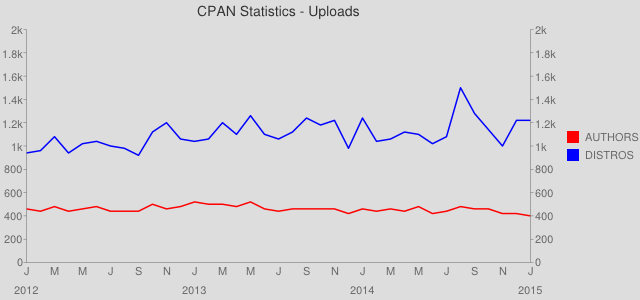
\includegraphics[width=10cm]{lectures/L1/stats6.png}
\end{figure}\noindent

К 2008 году по всему миру было собрано много групп Perl Mongers пытаясь противостоять вытеснению языка perl. В 2014 году их было примерно 256 групп, 8 из них в России. Эти цифры уже ушли в историю, но о их нельзя было не заметить.

\begin{figure}[H] \centering
  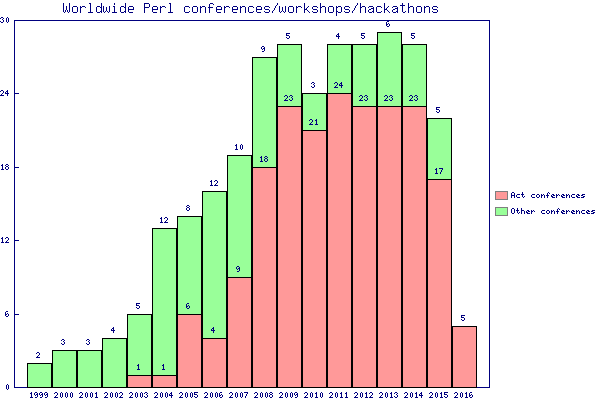
\includegraphics[width=10cm]{lectures/L1/act-conferences.png}
\end{figure}\noindent

\verb|act| - конференции программа которых зарегистрирована и размещена на официальном сайте Moungers групп.

На конференции O'Reilly's Money по финансовым технологиям в Нью-Йорке в 2008 году подсчитали количество упоминаний докладчиками базовых технологий.

Топ 3:
\begin{itemize}
 \item Перл
 \item SQL
 \item XML
\end{itemize}

И еще немного статистических данных:

На конец 2015 года было 600 000 уникальных посетителей CPAN в месяц. По грубым оценкам в мире на 1000 человек 1 программист ~6,5 миллионов программистов. Из этого можно примерно посчитать что 1 из 10-20 пишет на Perl. И не просто пишет, а заливает свои наработки в общую библиотеку модулей.


\subsection{Рынок труда}

Публикуемые вакансии:
\begin{figure}[H] \centering
  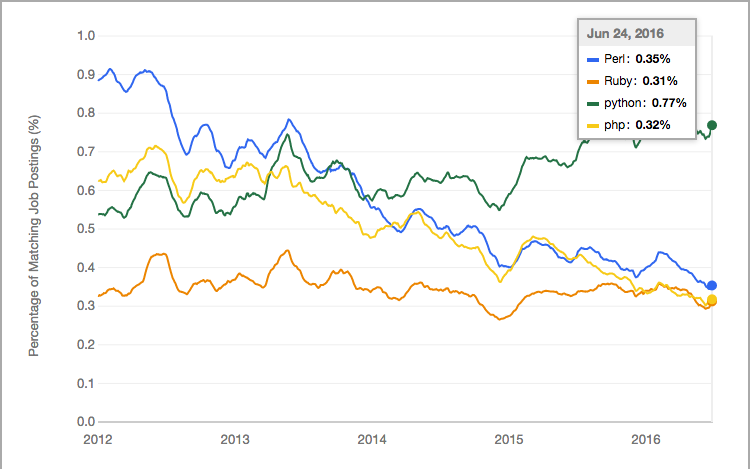
\includegraphics[width=10cm]{lectures/L1/jobgraph.png}
\end{figure}\noindent

Отношение публикуемых вакансий к соискателям:
\begin{figure}[H] \centering
  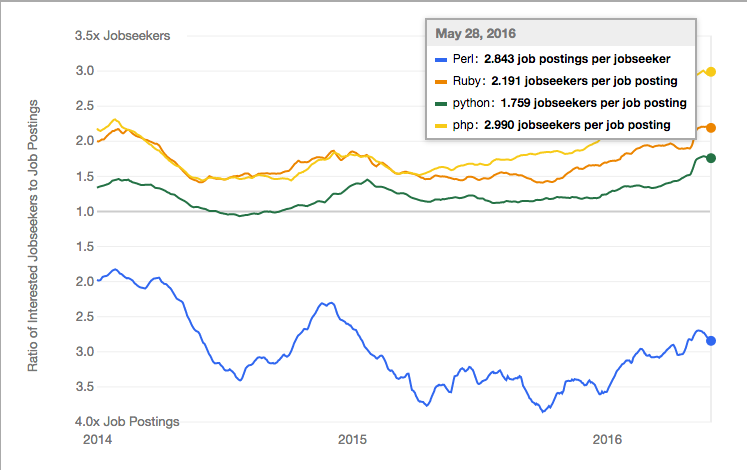
\includegraphics[width=10cm]{lectures/L1/jobgraph1.png}
\end{figure}\noindent

Зарплаты
\begin{figure}[H] \centering
  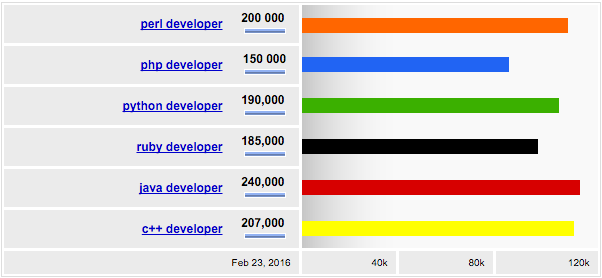
\includegraphics[width=10cm]{lectures/L1/zp.png}
\end{figure}\noindent

\subsection{Итог}
На сегодняшний день мы имеем:
\begin{itemize}
 \item  хорошо зарекомендовавший себя язык
 \item Огромную быстро растущую библиотеку
 \item Большое, активное сообщество
 \item Язык Perl6 и его отличный прототип, который вносит свои коррективы в развитие perl5
 \item идею сделать perl7, который быстро попадёт в продакшин, основываясь на опыте создания perl6 и надобности perl5
 \item Высокие зарплаты
\end{itemize}


\section{Настройка окружения}
\subsection{Настройка окружения в Mac OS}
Сам perl уже предустановлен (узнать версию можно, если набрать \verb|perl -v| в командной строке), но для сборки сторонних XS-модулей придётся установить xcode, <<Command line tools>>. Также, возможно, придется использовать macports (это perl установленный в отдельную директорию, отличный от системного).

Подробнее про установку можно прочитать в perldoc \perldoc{perlmacosx}.

\subsection{Настройка окружения в Linux}
Как правило перл есть в репозиториях дистрибутива. Команды для установки для некоторых дистрибутивов:
\begin{itemize}
 \item для CentOS: \verb|yum install perl| (Как правило в CentOS версия perl обновляется крайне редко. Поэтому, если необходима более современная версия, ее придется собирать самостоятельно.)
 \item для Debian: \verb|apt-get install perl|
 \item для GenToo: \verb|emerge dev-lang/perl|
 \item для FreeBSD: \verb|pkg add perl|
\end{itemize}
Сборки Perl есть почти под все операционные системы, даже под некоторые микроконтроллеры. Чтобы самостоятельно собрать perl, нужно скачать исходный код и выполнить:
\begin{minted}{bash}
make perl ./Configure -des; make test instal
\end{minted}
Если нужно установить его в другую директорию, нужно указать это с помощью ключей для make.

\subsection{Настройка окружения в Windows}
Для Windows существует несколько дистрибутивов Perl:
\begin{itemize}
  \item \textbf{ActivePerl от ActiveState}. Фирма ActiveState знаменита тем, что сделала Perl продакшн-системой, модули для которой они продавали.
  \item \textbf{StrawberryPerl} (рекомендуется использовать). В отличие от ActivePerl, StrawberryPerl идёт сразу с компилятором mingw, а также существенно удобнее и проще установка модулей.
  \item \textbf{cygwin}
\end{itemize}
С ActivePerl надо позаботится о наличие nmake + win32GnuUtils иначе сборка модулей будет мучительной и утомляющей.


\subsection{Проверка доступности интепретатора}
Чтобы проверить доступность интерпретатора, необходимо набрать в терминале:
\begin{minted}{bash}
  perl -v
\end{minted}
Выдача будет примерно такой:
\begin{minted}{bash}
This is perl 5, version 18, subversion 2 (v5.18.2) built for
x86_64-linux-gnu-thread-multi
(with 40 registered patches, see perl -V for more detail)

Copyright 1987-2013, Larry Wall

Perl may be copied only under the terms of either the Artistic License or the
GNU General Public License, which may be found in the Perl 5 source kit.

Complete documentation for Perl, including FAQ lists, should be found on
this system using "man perl" or "perldoc perl".  If you have access to the
Internet, point your browser at http://www.perl.org/, the Perl Home Page.
\end{minted}

Если вместо этого выводится ошибка <<Command not found>> или какая-то другая, то с установкой, что то пошло не так. Возможно, интерпретатор находится за пределами возможных путей из переменной окружения среды PATH.

\section{Базовый синтаксис языка Perl}
Синтаксис языка Perl близок к синтаксису языка C, а также в нем реализованы идеи и конструкции из shell, awk (популярная утилита для работы с табличными данными), sed и так далее.

\subsection{Простые конструкции в Perl}
Каждая программа на Perl представляет собой последовательность утверждений (statement). Комментарии в языке Perl начинаются с символа \verb|#|.
\begin{minted}{perl}
$a = 42;
say "test";
eval { ... };
do { ... };
my $var;
# Комментарий
\end{minted}
Каждое утверждение возвращает некоторое значение.
\begin{minted}{perl}
# Простые конструкции возвращают значение
$a = 42;        # => 42
say "test";     # => 1
eval { 7 };     # => 7
do { 1; 2; 3 }; # => 3
my $var;        # => undef
\end{minted}
Если утверждение --- это вызов функции, то возвращается значение, которое было возвращено функцией. Если утверждение --- это присвоение переменной некоторого значения, то возвращается значение этой переменной.

\subsection{Инициализация переменных. Режим strict}
Следует отметить, что Perl --- нетипизированный язык, любой переменной можно присвоить значение любого типа. Одна и та же переменная в различных участках программы может принимать значения разных типов.

Одна из особенностей Perl заключается в том, что новые переменные инициализируются автоматически в момент первого использования. Это было очень удобно для создания программ-однострочников, но создавало массу проблем в крупных проектах, когда при опечатке в имени какой-либо переменной Perl просто создавал еще одну переменную при этом менялась логика работы программы, но ошибка оставалась незамеченной и найти её было крайне сложно.

Поэтому в Perl появилась специальная директива strict, которая включает так называемый строгий режим. В этом режиме все переменные должны быть явно инициализированы до их первого использования. В ином случае на этапе компиляции кода выводится исключение о том, что была попытка использовать не объявленную переменную. Инициализация переменной происходит с помощью функции my. Хорошим тоном считается писать все программы (длиной более строчки) в режиме strict.

\subsection{Блоки. Область видимости переменной}
Блоком (scope) называется все, что заключено в фигурные скобки:
\begin{minted}{perl}
{
statement;
statement;
...
}
\end{minted}
Переменные, объявленные внутри такого блока, не видны за его пределами. Это свойство позволяет локализовывать части кода.


\subsection{Управляющие конструкции}
В Perl доступны следующие управляющие конструкции:
\begin{itemize}
  \item \textbf{Условия:} \verb|if|, \verb|unless|, \verb|elsif|, \verb|else|
  \begin{minted}{perl}
    if     ( EXPR ) { ... }
    elsif  ( EXPR ) { ... }
    else            { ... }
  \end{minted}
  С помощью \verb|else| и \verb|elsif| (именно так, а НЕ \verb|elseif| или \verb|else if|) можно указать, что должно быть выполнено, если условие не выполнено. Команда \verb|elsif|, в отличие от \verb|else|, сначала проверяет другое условие. Если условие выполняется, то исполняется код в фигурных скобках, а в ином случае программа переходит к следующему \verb|elsif| или  \verb|else|, если они есть.

  Такой же синтаксис и у команды \verb|unless|:
  \begin{minted}{perl}
      unless ( EXPR ) { ... }
  \end{minted}
  В этом случае код в фигурных скобках выполняется только, если выполнено условие в круглых скобках. При этом плохим тоном считается использование конструкций такого вида:
  \begin{minted}{perl}
      unless ( EXPR ) { ... }
      elsif  ( EXPR ) { ... }
      else            { ... }
  \end{minted}

  \item \textbf{Циклы:} \verb|while|, \verb|until|, \verb|for|, \verb|foreach|
  \begin{minted}{perl}
  while ( EXPR ) { ... }
  \end{minted}
  Оператор \verb|while| исполняет код в теле цикла, пока выполнено некоторое условие. Использование ключевого слова \verb|continue| позволяет указать блок кода, который будет выполнен всегда после каждой итерации. Например, если был совершен преждевременный выход из цикла, блок \verb|continue| все равно будет выполнен. Оператор \verb|until| имеет похожий синтаксис, но выполняет код в теле цикла, пока условие не выполнено:
  \begin{minted}{perl}
  until ( EXPR ) { ... } continue { ... }
  \end{minted}
  Еще два оператора for и foreach являются синонимами в Perl и позволяют итерировать по значениям целочисленной переменной и по элементам списка:
  \begin{minted}{perl}
  for ( EXPR; EXPR; EXPR ) { ... }
  for ( LIST ) { ... }
  for VAR ( LIST ) { ... } # Объявляется переменная, которая будет доступна в обоих scope.
  for VAR ( LIST ) { ... } continue { ... }
  \end{minted}
  \item \textbf{Выбор:} \verb|given|, \verb|when|
  \item \textbf{Безусловный переход:}  \verb|goto|
\end{itemize}

\subsection{Типы данных в Perl}
Основные типы данных в Perl включают в себя:
\begin{itemize}
  \item \textbf{SCALAR}~--- простая переменная, имя всегда начинается с символа \verb|$|, может содержать одно из следующих значений:
  \begin{itemize}
    \item \textbf{Number} (числовое значение): \verb|$s = 1|, \verb|$s = -1e30|.
      Perl работает с числовыми значениями как с числами (то есть быстро) до тех пор, пока не будет к ним обращения как к строке. В последнем случае числовое значение будет преобразовано в строковое.

    \item \textbf{String} (строковое значение): \verb|$s = "str"|. Строка в Perl всегда обрамлена в кавычки.
    \item \textbf{Reference} (ссылка): разыменовывание ссылки \verb|$r| делается в зависимости от того типа данных, который предпологается, что лежит по ссылке:
      \begin{itemize}
        \item \textbf{Scalar} (\verb|$$r|, \verb|${ $r }|)
        \item \textbf{Array} (\verb|@$r|, \verb|@{ $r }|, \verb|$r->[...]|)
        \item \textbf{Hash} (\verb|%$r|, \verb|%{ $r }|, \verb|$r->{...}|)
        \item \textbf{Function} (\verb|&$r|, \verb|&{$r}|, \verb|$r->(...)|)
        \item \textbf{Filehandle} (\verb|*$r|)
        \item \textbf{Lvalue} (\verb|$$r|, \verb|${ $r }|)
        \item \textbf{Reference} (\verb|$$r|, \verb|${ $r }|)
      \end{itemize}
    Нужно иметь в виду, что, если разыменовать ссылку на хэш как массив, получится каша, а именно: получится массив из поочередно ключей и соответствующих значений.
  \end{itemize}
  \item \textbf{ARRAY} (\verb|@a|, \verb|$a[...]|)
  \item \textbf{HASH} (\verb|%h|, \verb|$h{key}|, \verb|$h{...}|)
\end{itemize}


\subsection{Специальные переменные}
В perl существуют специальные глобальные переменные, которые позволяют существенно упростить написание программ:
\begin{itemize}
  \item \verb|$_|, \verb|$ARG| --- аргумент по умолчанию,
  \item \verb|@_|, \verb|@ARG| --- аргументы функции (как массив).
  \item \verb|$a|, \verb|$b| --- переменные, используемые при сортировке:
  \begin{minted}{perl}
  for (sort { $a <=> $b } @ARGV) {
  say "Arg: $_";
  }
  say "Was run by $ENV{USER}";
  \end{minted}
  Поэтому при написании программы категорически не рекомендуется заводить переменные с такими же именами.
  \item \verb|%ENV| --- переменные окружения (как хэш),
  \item \verb|@ARGV| --- аргументы программы (как массив).
\end{itemize}
Также существуют следующие специальные переменные:
\begin{itemize}
  \item \verb|$"|, \verb|$LIST_SEPARATOR| --- разделитель при интерполяции в кавычках.
  \item \verb|$,|, \verb|$OUTPUT_FIELD_SEPARATOR| --- разделитель между элементами списка при выводе (при выводе на экран массива его элементы будут разделены этим символом)
  \item \verb|$/|, \verb|$INPUT_RECORD_SEPARATOR| --- разделитель входного потока для readline
  \item \verb|$\|, \verb|$OUTPUT_RECORD_SEPARATOR| --- разделитель выходного потока для print
  \item \verb|$.|, \verb|$INPUT_LINE_NUMBER|
\end{itemize}
Пример использования:
\begin{minted}{perl}
$" = "."; # $LIST_SEPARATOR
$, = ";"; # $OUTPUT_FIELD_SEPARATOR
$\ = "\n\n"; # $OUTPUT_RECORD_SEPARATOR
while (<>) {
    chomp;
    @a = split /\s+/, $_;
    say "$. @a",@a;
    }
\end{minted}
Есть еще ряд специальных переменных:
\begin{itemize}
  \item \verb|$!|,  \verb|ERRNO|~--- переменная в которую записываются ошибки при открытии файлов.
  \item \verb|$<|,  \verb|UID|~--- ID пользователя, запустившего программу.
  \item \verb|$$|,  \verb|PID|~--- PID процесса
  \item \verb|$0|,  \verb|PROGRAM_NAME|~--- Имя программы
  \item \verb|$^X|,  \verb|EXECUTABLE_NAME|~--- название запущенного бинарного файла
  \item \verb|$^O|,  \verb|OSNAME|~--- имя используемой операционной системы
  \item \verb|$^V|,  \verb|PERL_VERSION|~--- версия perl
\end{itemize}

Например:
\begin{minted}{perl}
say "I'm $^X, $^V, on $^O";
say "Script: $0 (@ARGV);";
say "Pid $$ by uid $<";
open my $f, '<','/etc/shadow'
or die "No shadow: $!\n";
\end{minted}

\begin{minted}{bash}
/usr/bin/perl sample.pl -test
\end{minted}

\begin{verbatim}
# I'm /usr/bin/perl, v5.18.2, on darwin
# Script: sample.pl (-test);
# Pid 70032 by uid 502
# No shadow: No such file or directory
\end{verbatim}

\section{Запуск однострочных скриптов}
Perl в начале своего развития использовался для запуска и исполнения простейших однострочных скриптов. Также, за исключением небольшого числа системнозависимых библиотек, Perl на всех операционных системах работает одинаково. Именно поэтому Perl был так популярен среди системных администраторов.

При написании однострочников \verb|use strict;| писать необязательно. Но если вдруг скрипт начал выполнять не то, что задумано, лучше добавить \verb|use strict;|, что упростит отладку.

Запустить однострочник можно с помощью ключа \verb|-e|, после которого идет код однострочника в кавычках:
\begin{minted}{bash}
perl -e 'print "Hello world\n"'
\end{minted}
Использовать всегда следует одинарные кавычки, так как разные шеллы по-разному работают с двойными кавычками, и существует соглашение, что одинарные кавычки --- неинтерполируемые (то есть в них не будут подставляться переменные среды). Обычно однострочная программа, обрабатывает данные приходящие ей в стандартном вводе. Вот простейшая программа которая читает стандартный ввод и распечатывает строки добавляя в начало каждой из них дефис
\begin{minted}{bash}
perl -e 'while(<>){print "- ".$_}'
\end{minted}
Чтобы постоянно не использовать конструкцию \verb|while(<>){}| при выполнении действия над каждой строчкой в файле, существует ключ \verb|-n|. Идентичная запись той же программы:
\begin{minted}{bash}
perl -ne 'print "- ".$_'
\end{minted}
Внутри цикла \verb|while(<>){}| переменная \verb|$_| будет содержать цельную строку вместе с символом \verb|\n|. Что бы не использовать команду chomp (отрезающую в конце перенос строки) можно использовать флаг \verb|-l|, который:
\begin{itemize}
  \item устанавливает переменную \verb|$\| (разделитель, который выведен после каждого выполнения команды print)
  \item устанавливает переменную \verb|$/| (разделитель по которому будет делится входящий поток, отдельно его можно выставить с помощью флага \verb|-0|)
  \item удаляет из строки \verb|$_| последний перенос строки (при совместном использовании с флагом \verb|-n|)
\end{itemize}
Например, прочитать файл в котором записи разделены через \verb|";"| и вывести каждую запись на новой строке можно так:
\begin{minted}{bash}
perl -nl00120073 -e 'print $_'
\end{minted}
Все строки из файла записать через \verb|";"| можно так:
\begin{minted}{bash}
perl -nl00730012 -e 'print $_'
\end{minted}
Флаг \verb|-p| делает тоже самое, что и флаг \verb|-n|, только в каждую итерацию цикла добавит еще вывод переменной \verb|$_|:
\begin{minted}{bash}
perl -nl00120073 -e ''
\end{minted}
\begin{minted}{bash}
perl -pl00730012 -e ''
\end{minted}
Детальнее можно посмотреть тут: perldoc \perldoc{perlvar}.

Для парсинга более сложных структур файлов (например, когда в каждой строке есть записи разделенные определённым разделителем), можно использовать флаг  \verb|-a| совместно с \verb|-F|:
\begin{itemize}
  \item Флаг \verb|-a| добавляет функцию разделяющую входную строку на части и складывает в спецмассив \verb|@F|
  \item \verb|-F| устанавливает разделитель (по умолчанию это пробел)
\end{itemize}
Например, с помощью следующего кода можно прочитать файл-таблицу, в которой каждая строка представляет собой набор полей разделенных \verb|";"|, проверить третью колонку на наличие там 1 и при выполнении условия вывести значение из 2 колонки:
\begin{minted}{perl}
perl -lnaF';' -e 'if( $F[2] == 1 ){ print $F[1] };'
\end{minted}
В этом примере флаг \verb|-l| необходим, чтобы выполнять скрипт для каждой строки файла.

\subsection{Система CPAN}
Perl завоевал к себе доверие, за счет того, что был портирован под всевозможные платформы и системы, а также за счет большой системы CPAN. CPAN --- архив модулей, написанных на языке программирования Perl.
Все версии модулей под все версии perl проходят тестирование (разработчик модуля должен сам должен предоставить тесты) автоматической системой на CPAN. Эта система запускает модуль на каждой версии perl и отмечает результат выполнения тестов в специальной таблице. Часто при крупных обновлениях perl некоторые модули перестают работать, поэтому при выборе модуля для работы эта таблица может оказаться полезной.

\begin{figure}[H] \centering
  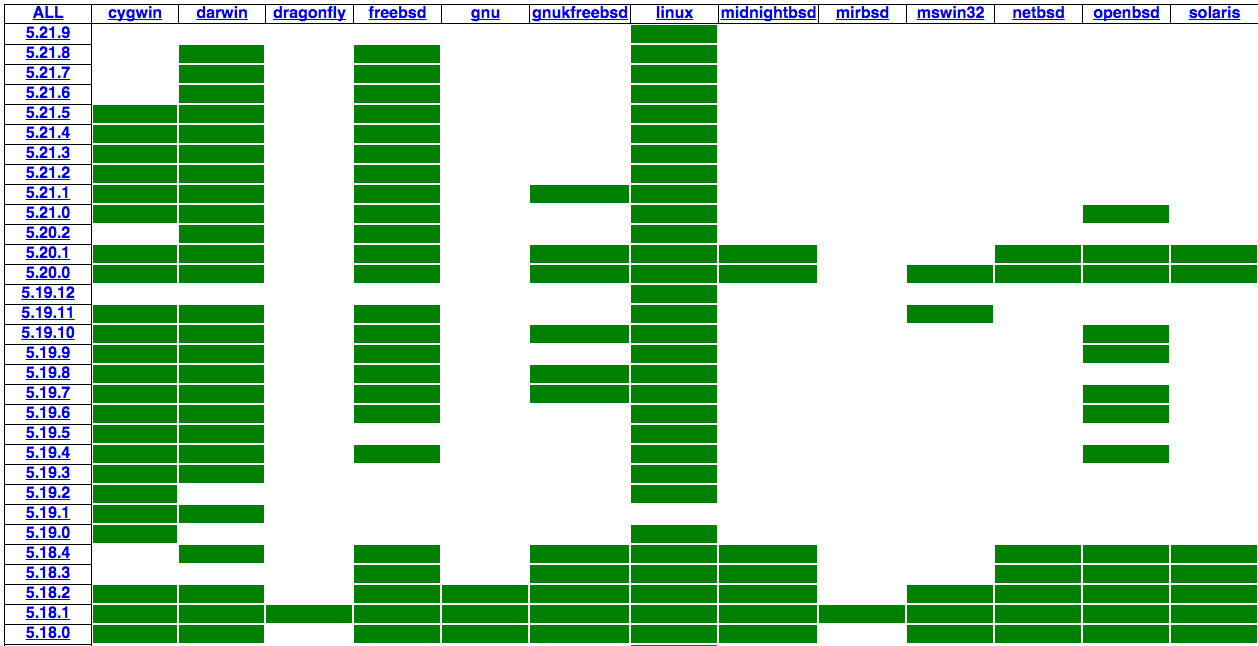
\includegraphics[width=10cm]{lectures/L1/matrixcpantesters.png}
\end{figure}\noindent

Подключить модули (чтобы иметь возможность пользоваться функциями этого модуля) можно опцией \verb|-M|, например:
\begin{minted}{perl}
perl -MJSON::XS -e 'print JSON::XS::encode_json({var1 => 1, var2 => 2})'
\end{minted}
Perl поддерживает еще много других ключей, но представленных должно быть достаточно для начала изучения языка.

\section{Средства отладки в Perl}
\subsection{Доступ к кодам операции}
В perl 5 (начиная с версии 5.005) был обеспечен доступ к компилятору. По умолчанию Perl переводит исходный код в коды операции и исполняет их. Если вы не хотите выполнять свою программу, а хотите проанализировать коды операции, то можно написать собственный модуль или воспользоваться существующим. Для таких модулей было выделено пространство имен \verb|B::|). Доступ к компилятору организован, через модуль \verb|O|, таким образом для передачи кодов операций в некоторый модуль для их анализа, следует использовать модуль \verb|O|, передавая ему имя модуля для получения кодов операций:
\begin{minted}{perl}
perl -MO=Backend
\end{minted}
Указанный модуль может вывести коды операций на экран, проанализировать быстродействие. Эта функция будет особенно полезна при отладке. Например, \verb|B::Concise| --- модуль, позволяющий вывести коды операции как есть.

\subsection{Модуль Deparse}
\verb|B::Deparse| --- модуль, который превращает коды операции после компилятора обратно в код на perl, то есть декомпилирует коды операций. У этого модуля есть множество опций, позволяющих менять его поведение.

Работу модуля можно продемонстрировать на программе
\begin{minted}{perl}
perl -pl00730012 -e ''
\end{minted}
запуская perl с подключенным модулем B::Deparse:
\begin{minted}{perl}
perl -MO=Deparse -pl00730012 -e ''
\end{minted}
На выходе получается:
\begin{minted}{perl}
BEGIN { $/ = "\n"; $\ = ";"; }
LINE: while (defined($_ = <argv>) ){
    chomp $_;
}
continue {
    die "-p destination: $!\n" unless print $_;
}
-e syntax OK
\end{minted}
У модуля B::Deparse есть свои удобные ключи:
\begin{itemize}
  \item \verb|-l| добавит комментарии с ссылками на строки исходного файла
  \item \verb|-p| расставит скобки и тем самым покажет приоритетность выполнения команд
  \item \verb|-q| развернёт интерполируемые строки, то есть представит их как конкатенацию неинтерполируемых строк и переменных. Интерполирование строк --- это поиск внутри строчек, которые обрамлены в двойные кавычки, имен переменных и замена их на соответствующие им значения:
  \begin{minted}{perl}
  "Hello $name" = 'Hello ' . $name != 'Hello $name'
  \end{minted}
  Строки в одинарных кавычках не интерполируются.
  \item Ключ \verb|-sС| определяет стиль вывода кода.
  \item Ключ \verb|-siNUMBER| определяет количество пробелов в отступе
  \item Ключ \verb|-siT| позволяет использовать символ табуляции
  \item Ключ \verb|-xNUMBER| определяет уровень развертывания кода
\end{itemize}
\verb|B::Deparse| можно использовать, как обычный модуль, передавая ему ссылку на функцию, код которой хочется посмотреть (в том числе, если доступна только ссылка на функцию):
\begin{minted}{perl}
use B::Deparse;
sub func {
    print 'Hello world!!!'
};

my $deparse = B::Deparse->new("-p", "-sC");
$body = $deparse->coderef2text(\&func);

print $body;
\end{minted}
После выполнения такой программы:
\begin{minted}{perl}
{
print('Hello world!!!');
}
\end{minted}

При уровне отладки большем чем 3 все циклы for будут развёрнуты в while. Код:
\begin{minted}{bash}
perl -MO=Deparse,x3 -e 'for ($i = 0; $i < 10; ++$i) {print $i;}'
\end{minted}
Превратится в
\begin{minted}{perl}
$i = 0;
while ($i < 10) {
    print $i;
} continue {
    ++$i
}
\end{minted}
\subsection{Data::Dumper}
\verb|Data::Dumper| - модуль, который поможет выводить на экран в развернутом виде сложные структуры данных. Например:
\begin{minted}{perl}
use Data::Dumper;
my $foo = [{a => 1, b => 2},{c => 3, d => 4}];
print Dumper($foo);
\end{minted}
Вот так красиво демонстрирует эту переменную \verb|Data::Dumper|:
\begin{minted}{perl}
$VAR1 = [
    {
      'b' => 2,
      'a' => 1
    },
    {
      'c' => 3,
      'd' => 4
    }
];
\end{minted}
У \verb|Data::Dumper| есть множество опций, которые позволяют управлять стилем вывода: табуляцией, переносом строк и так далее.

\subsection{Модуль DDP (Data::Printer)}
Есть альтернативный модуль для просмотра структур и объектов. Его обычно используют для отладки приложений. У этого модуля не меньше настроек, чем у Data::Dumper, но его проще использовать, например:
\begin{minted}{perl}
use DDP;
my $foo = {a=>1, b=> 2, c=> [1,2,3]};
p $foo;
\end{minted}
Вывод следующий:
\begin{minted}{perl}
\ {
    a   1,
    b   2,
    c   [
        [0] 1,
        [1] 2,
        [2] 3
    ]
}
\end{minted}
Модуль DDP в основном отличается от Data::Dumper следующим:
\begin{itemize}
  \item Автор этого модуля позаботился о цветовой разметке выводимых данных, для удобства чтения.
  \item Так же у этого модуля более расширенный дамп объектов:
  \begin{minted}{perl}
  \ SomeClass  {
    Parents       Moose::Object
    Linear @ISA   SomeClass, Moose::Object
    public methods (3) : bar, foo, meta
    private methods (0)
    internals: {
      _something => 42,
    }
  }
  \end{minted}
  \item Отсутствует сериализация.
\end{itemize}

\subsection{Использование отладчика}
Для начала работы с дебагером рекомендуется прочитать документацию \perldoc{perldebtut}. Отладка программ подразумевает построчное их выполнение с возможностью просмотра состояния переменных между ними.

Запуск отладчика выполняется добавлением ключа \verb|-d| при запуске интерпретатора:
\begin{minted}{perl}
perl -d myscript.pl
\end{minted}
Для того, что бы отладчик запустился скрипт не должен содержать синтаксических ошибок и должен нормально компилироваться через \verb|perl -c|. После запуска отладчика на экране появится:
\begin{minted}{bash}
Loading DB routines from perl5db.pl version 1.44
Editor support available.

Enter h or 'h h' for help, or 'perldoc perldebug' for more help.

DB<1>
\end{minted}
Далее отладчик ждёт команд. Некоторые команды отладчика для просмотра кода и значения переменных:
\begin{verbatim}
- l посмотреть код. Параметра можно указать номер строки, номер строки + интервал, диапазон строк, название функции. На выход вы получаете запрошенный код
- - посмотреть предыдущий код относительно текущей строки
- v посмотреть код вокруг указанной строки
- / поиск по коду в прямом направлении на вход эта команда принимает регулярное выражение, если ничего не передавать то отладчик продолжит поиск по предыдущему запросу
- ? поиск по коду в обратном направлении
- f загрузка файла для просмотра, на вход принимает имя файла
- . вернуть указатель на текущую позицию выполнения кода
- m $obj показать все методы объекта
- M показать список всех загруженных модулей
- S список всех доступных функций в данной точке
- [X|V] [Package] [str|~re] список переменных. Можно передать имя пакета внутри которого интересуют переменные, название переменно или регулярное выражение для названия переменной
\end{verbatim}
Команды отладчика для выполнения кода:
\begin{verbatim}
- p выполнить перл выражение и показать результат
- n шаг вперёд без захода в процедуру
- s шаг вперёд с заходом в процедуру
- T стек вызовов в данной точке
- ! повторить предыдущую команду. На вход можно передать номер команды в истории которую надо повторить
- source file - выполнить команды из файла
- с продолжить выполнение программы. Если параметром указать номер строки или имя функции, то отладчик продолжит выполнение до указанного места
- r продолжить выполнение скрипта до выхода из подпрограммы
- q выход из отладчика
\end{verbatim}
Точки останова, действия, точки наблюдения
\begin{verbatim}
- b < line|sub > [условие] - установить точку останова на указанную строку или функцию при выполнении условия
- B < ln|* > - снять точку останова
- a строка действие [условие] - установить действие которое сработает достигнув определённой строки
- A < line|* > - удалить действие
- w $var - установить наблюдение за переменной
- W $var|* - снять наблюдение за переменной
- L [a|b|w] - вывести список точек останова, действий, наблюдений за переменными
- R - начать скрипт заново оставив все точки останова, действия, наблюдения
\end{verbatim}

\subsection{Использование отладчика: пример}
В качестве примера будет показана отладка следующего скрипта:
\begin{minted}{perl}
use strict;

my $ret = 0;

foreach ( my $i = 0 ; $i < 50 ; $i++ ) {
    if ( $ret > $i ) {
        $ret -= $i;
    }
    else {
        $ret += $i;
    }
}
print $ret;
\end{minted}
Запуск отладки:
\begin{minted}{bash}
perl -d mydebug.pl
\end{minted}
Отладчик запустился и выдал приглашение:
\begin{minted}{bash}
Loading DB routines from perl5db.pl version 1.44
Editor support available.

Enter h or 'h h' for help, or 'perldoc perldebug' for more help.

main::(mydebug.pl:3):   my $ret = 0;

DB< 1 >
\end{minted}
Команда \verb|l| позволяет просмотреть код с указанием текущей позиции:
\begin{minted}{perl}
3==>    my $ret = 0;
4:      my $cnt_add = 0;
5:      my $cnt_sub = 0;
6
7:      foreach(my $i = 0; $i < 50; $i++){
8:              if($ret>$i){
9:                      $ret -= $i;
10              }
11              else {
12:                     $ret += $i;
\end{minted}
Установка точки останова (команда \verb|b|) на 8ой строчке при достижении 10 итерации цикла:
\begin{minted}{bash}
b 8 $i == 9
\end{minted}
Запуск программы (команда \verb|c|)
\begin{minted}{bash}
c
\end{minted}
Когда выполнится условие \verb|$i == 9|, сработает точка останова и на экране появится сообщение:
\begin{minted}{bash}
DB< 7 >
c
main::(mydebug.pl:8):           if($ret > $i){
\end{minted}
Вывод значения переменной \verb|$i|:
\begin{minted}{bash}
DB< 7 > print $i
9
\end{minted}
Отслеживать переменные можно командой \verb|$w|:
\begin{minted}{bash}
w $ret
\end{minted}
После этого выполнив 1 строчку (команда \verb|n|):
\begin{minted}{bash}
DB< 9 >
n
Watchpoint 0:   $ret changed:
old value:  ''
new value:  '16'
main::(mydebug.pl:9):                   $ret -= $i;

DB< 9 >
\end{minted}
Дальнейшая отладка происходит по тем же принципам.

%\setcounter{chapter}{1}
\chapter{Синтаксис и типы данных}
Про язык Perl существует миф, что это write-only язык. Это связано с тем, что большинство использующих язык не всегда понимают, как он устроен.

Основной принцип, заложенный в язык Perl, это TIMTOWTDI (There's More Than One Way To Do It), то есть существует множество вариантов, как реализовать одно и то же. Использовать при написании программы следует тот вариант, который лучше всего читается. В ином случае, действительно, получившуюся программу сможет прочесть только интерпретатор (<<The only thing can parse Perl (the language) is perl (the binary).>>).

\section{Базовый синтаксис}
\subsection{Блок}
Блок --- последовательность утверждений, отделенная ограничителями (фигурными скобками):
\begin{minted}{perl}
{
	statement;
	statement;
	...
}
\end{minted}

Не всегда код, отделенный фигурными скобками, является блоком. Так, например, в случае оператора \verb|do {...}| фигурные скобки --- часть синтаксиса, а не выделение блока:
\begin{minted}[escapeinside=||]{perl}
do { ... } |$\ne$| { ... }
\end{minted}
Оператор \verb|do| выполняет код внутри фигурных скобок и возвращает значение:
\begin{minted}{perl}
$value = do { ... }
\end{minted}
Блок же никакое значение не возвращает:
\begin{minted}{perl}
# НЕВЕРНО: *$value = { ... };
\end{minted}
Блок может использоваться для задания области видимости переменных.

\subsection{Управление циклами}
Существуют следующие управляющие конструкции:
\begin{itemize}
  \item \verb|next| (аналог continue из C) позволяет пропустить оставшиеся в теле цикла утверждения и перейти к началу блока continue (если он есть) или к выполнению следующей итерации цикла.
  \begin{minted}{perl}
  for my $item ( @items ) {
      my $success = prepare($item);

      unless ($success) {
          next;
      }

      process($item);
  } continue {
      # next переходит сюда
      postcheck($item);
  }
  \end{minted}

  \item \verb|last| (аналог break из C) немедленно прекращает выполнение цикла (без выполнения блока continue).
  \begin{minted}{perl}
  for my $item ( @items ) {
      my $success = prepare($item);

      unless ($success) {
          last;
      }

      process($item);
  } continue {
      postcheck($item);
  }
  # last переходит сюда
  \end{minted}

  \item \verb|redo| начинает повторное выполнение тела цикла без изменения переменных состояния (не инициализируя следующую итерацию).
  \begin{minted}{perl}
  for my $item ( @items ) {
      # redo переходит сюда
      my $success = prepare($item);

      unless ($success) {
          redo;
      }

      process($item);
  } continue {
      postcheck($item);
  }

  \end{minted}
\end{itemize}
Блок идентичен одиночному циклу, а, следовательно, в нем работают эти же управляющие конструкции:
\begin{minted}{perl}
{
    # redo
    stmt;
    if (...) { next; }

    stmt;
    if (...) { last; }

    stmt;
    if (...) { redo; }

    stmt;
    # next
}
# last
\end{minted}

\subsection{Оператор выбора}
Пара \verb|given|/\verb|when| --- оператор выбора (в Си аналогичный оператор это switch/case). Оператор выбора доступен с версии 5.10.
\begin{minted}{perl}
use feature 'switch'; # v5.10 - v5.18

given ( EXPR ) {
    when ( undef )    { ... }
    when ( "str" )    { ... }
    when ( 42 )       { ... }
    when ( [4,8,15] ) { ... }
    when ( /regex/ )  { ... }
    when ( \&sub )    { ... }
    when ( $_ > 42 )  { ... }
    default           { ... }
}
\end{minted}
Внутри when (...) вызывается оператор smartmatch. Это позволяет использовать сложные конструкции при поиске совпадения. Подробнее смотрите \href{http://perldoc.perl.org/functions/given.html}{документацию}. В отличие от других языков, по умолчанию исполняется только часть кода, соответствующая подходящему условию. Не нужно использовать ключевое слово \verb|break| (как бы автоматически подразумевается в конце каждого \verb|when|), чтобы избежать <<проваливания>> в следуюющую за ней часть. Для такого <<проваливания в следующий when>> используется ключевое слово \verb|continue|.

\subsection{Переход (goto)}
Конструкция \verb|goto| имеет множественное поведение. В самом простом случае goto обеспечивает переход на метку:
\begin{minted}{perl}
goto LABEL;
\end{minted}
Например:
\begin{minted}{perl}
LABEL1:
    say "state 1";
    goto LABEL2;
LABEL2:
    say "state 2";
    goto LABEL1;
\end{minted}
Получается бесконечная программа:
\begin{minted}{bash}
state 1
state 2
state 1
state 2
...
\end{minted}
Существует устаревший синтаксис (его не следует использовать в новых программах --- будет выводиться предупреждение об использовании устаревших возможностей):
\begin{minted}{perl}
goto EXPR; # DEPRECATED
\end{minted}
В этом случае в качестве параметра передается строка и имя строки будет воспринято как метка:
\begin{minted}{perl}
{
EVEN:
    say "even";
    last;
ODD:
    say "odd";
    last;
}

goto(
    ("EVEN","ODD")[ int(rand 10) % 2 ]
);
\end{minted}

\subsection{Хвостовой вызов}
Также goto может использоваться для обеспечения хвостового вызова, который позволяет вызвать тело другой функции на месте данной с теми же аргументами, которые были переданы данной фунции.
\begin{minted}{perl}
goto &NAME;
goto &$var;
\end{minted}
Например, следующий код вычисляет значение чисел Фибоначи с помощью рекурсии:
\begin{minted}{perl}
sub fib {
    return 0 if $_[0] == 0;
    return 1 if $_[0] == 1;
    return _fib($_[0]-2,0,1);
}

sub _fib { my ($n,$x,$y) = @_;
    if ($n) {
        return _fib( $n-1, $y, $x+$y );
    }
    else {
        return $x+$y;
    }
}
\end{minted}
Основная проблема с рекурсией --- слишком быстро заполняется стек. Этой проблемы можно избежать, если использовать хвостовой вызов:
\begin{minted}{perl}
sub fib {
    return 0 if $_[0] == 0;
    return 1 if $_[0] == 1;
    return _fib($_[0]-2,0,1);
}

sub _fib { my ($n,$x,$y) = @_;
    if ($n) {
        @_ = ( $n-1, $y, $x+$y ); goto &_fib;
    }
    else {
        return $x+$y;
    }
}
\end{minted}
Аналогичным образом можно написать код для расчета значения факториала:
\begin{minted}{perl}
sub fac {
    my $n = shift;
    return _fac($n,1);
}

sub _fac {
    my ($n,$acc) = @_;
    return $acc if $n == 0;
    @_ = ($n-1,$n*$acc);
    goto &_fac;
}
\end{minted}

\subsection{Постфиксная нотация}
Помимо классического синтаксиса для условий и циклов, в Perl доступна постфиксная нотация:
\begin{minted}{perl}
STMT if EXPR;
STMT unless EXPR;
STMT while EXPR;
STMT until EXPR;
STMT for LIST;
STMT when EXPR;
\end{minted}
Такая запись обычно используется, чтобы подчеркнуть, что утверждение важнее условия (в случае \verb|if|), которое в постфиксной нотации идет после него.

С помощью \verb|do| и \verb|while| (или \verb|until|) можно реализовать так называемый постфиксный цикл:
\begin{minted}{perl}
do {
    ...;
} while ( EXPR );

do {
    ...;
} until ( EXPR );

do {
    ...;
} for ( LIST );
\end{minted}
Однако в таком цикле не работаю функции управления циклом (\verb|next|,\verb|last|,\verb|redo|), а также нет блока continue. Это связано с тем, что фигурные скобки внутри \verb|do| --- не являются блоком.

\section{Типы данных}
\subsection{Идентификаторы переменных}
\begin{figure}[H]\centering
	  \begin{tikzpicture}[scale=1.4] \def\setpoints#1(#2)#3<#4,#5>#6 at (#7);{
		\path[shift={(#7)}]
		( 0     , 0      ) coordinate (#2)
		( 0.5*#4, 0      ) coordinate (#2_east)
		( 0     , 0.5*#5 ) coordinate (#2_north)
		(-0.5*#4, 0      ) coordinate (#2_west)
		( 0     ,-0.5*#5 ) coordinate (#2_south)
		( 0.5*#4, 0.5*#5 ) coordinate (#2_north_east)
		(-0.5*#4, 0.5*#5 ) coordinate (#2_north_west)
		( 0.5*#4,-0.5*#5 ) coordinate (#2_south_east)
		(-0.5*#4,-0.5*#5 ) coordinate (#2_south_west); }



\def\doit{\draw[latex-] (box_west) -- (s); \draw[-latex] (box_east) -- (e);}
\def\stepbl{\path (current)+(0,-7mm) coordinate (current);}
\def\dblock<#1>(#2){
		\setpoints (box) <30mm,6mm> at (current);
		\draw[fill={#1}] (box_south_west) rectangle (box_north_east) (box) node {#2};
		\doit\stepbl }
\def\dblockl<#1>(#2){
		\setpoints (box) <30mm,6mm> at (current);
		\setpoints (box_in)  <6mm,6mm> at ($(box_west)+(0.3,0)$);
		\draw[fill={#1}] (box_in_south_west) rectangle (box_in_north_east) (box_in) node {$\wedge$};
		\draw[-latex] (box_in_east) --+ (4mm,0);
		\setpoints (box_in)  <20mm,6mm> at ($(box_west)+(2,0)$);
		\draw[fill={#1}] (box_in_south_west) rectangle (box_in_north_east) (box_in) node {#2};
		\doit\stepbl }
\def\dsmallblock<#1><#2> (#3) at (#4);{ \setpoints (box) <#1> at (#4);
		\draw[fill={#2}] (box_south_west) rectangle (box_north_east);
		\draw (box) node {#3}; }
	
	\def\block#1(#2)#3<#4>[#5] at (#6);{
		\setpoints (#2) <#4> at (#6);
		\draw (#2_south_west) rectangle (#2_north_east) (#2) node {\texttt{#5}};
	}
	
	
%---------------------------------------------

\def\block#1(#2)#3<#4>[#5] at (#6);{
	\setpoints (#2) <#4> at (#6);
	\draw (#2_south_west) rectangle (#2_north_east) (#2) node {\texttt{#5}};
}
\def\arr<#1>{\textcolor{blue}{[}#1\textcolor{blue}{]}}
\def\h<#1>{\textcolor{blue}{\{}#1\textcolor{blue}{\}}}
\def\curv<#1>{\textcolor{red}{\{}#1\textcolor{red}{\}}}
\def\red|#1|{\textcolor{red}{#1}}	
	  \path (0,0) coordinate (current)
	  (1.5,-2.1) coordinate (s)
	  (7.5,-3.4) node[circle] (e) {\}};

	  \foreach \n in {$\$$,$@$,$\%$, $\&$, $*$} {\stepbl
	  	\dsmallblock<5mm,6mm><gray!20> (\n) at (current);
	  	\draw[latex-] (box_east) -- (s);	}
	  \path (4.5,0) coordinate (current);
	  \dblock<green!20>(BAREWORD)
	  \draw[-latex] (box_west) --+ (-3mm,0);
	  \draw (box_north_west) + (-3mm,0) rectangle ($(box_south_west)+(-32.5mm,0)$);
	  \draw (box_west) + (-17.5mm,0) node{[A-Za-z\_]+[A-Za-z0-9\_]*};
	  \dblockl<red!15>(Letter)
	  \dblock<red!15>(Punctuation)
	  \dblock<red!15>(Digits)
	  \path (2,-3.4) coordinate (s) (current)+(0,-3mm) coordinate (current);
	  \dblock<yellow!15>(statement)
	  \dblockl<red!15>(BAREWORD)
	  \dsmallblock<5mm,6mm><gray!20> ($\{$) at (2,-3.4);
	  \draw[-latex] (1.5,-2.1) -- (box_north);
	  \dsmallblock<5mm,6mm><gray!20> ($\}$) at (7.4,-3.4);
	  \dsmallblock<10mm,6mm><gray!20> (Sigil) at (1.5,-2.1);
	  \end{tikzpicture}
    \caption{Идентификатор переменной}
\end{figure}
Любой идентификатор переменной начитается с символа Sigil, который обозначает контекст обращения и может быть одним из следующих:
\begin{itemize}
  \item $\$$ соответствует скалярной переменной (скалярный контекст),
  \item $@$  соответствует массиву (списковый контекст),
  \item $\%$ соответствует ассоциативному массиву (хэшу),
  \item $\&$ соответствует указателю на функцию,
  \item $\$\#$ соответствует последнему элементу списка,
  \item $^{\ast}$ означает специальный тип glob.
\end{itemize}

После Sigil идет имя переменной. Обычно оно представляет собой так называемый BAREWORD. BAREWORD --- любое, начинающееся не на цифру, сочетание больших и маленьких букв, символа подчеркивания и цифр. После Sigil могут идти фигурные скобки, внутри которых записывается какое-либо утверждение. Примеры обычных переменных:
\begin{verbatim}
  - $var, @array, %hash, &func, *glob
  - ${var}, @{array}, %{hash}, &{func}, *{glob}
  - ${ "scalar" . "name" }, %{ "hash".$id }
\end{verbatim}
Также переменная может быть одной из спецпеременных (на рисунке отмечены красным, полный список в \perldoc{perlvar}). Примеры специальных переменных:
\begin{minted}{perl}
  - $^W, $^O, $^X, ${^W}, ${^O}, ${^X}, ...
  - $0, $1, $100, ${0}, ${1}, ${100}, ...
  - ${^PREMATCH}, ${^MATCH}, ${^POSTMATCH}, ...
  - $_, @_, $!, $@, $?, $", $/, $,, ...
  - ${_}, @{_}, ${!}, ${@}, ${?}, ${"}, ${/}, ${,}, ...
\end{minted}

\subsection{SCALAR}
Переменная может быть числом. Числа записываются множеством способов:
\begin{minted}{perl}
$int         = 12345;
$pi          = 3.141592;
$pi_readable = 3.14_15_92_65_35_89;
$plank       = .6626E-33;
$hex         = 0xFEFF;
$bom         = 0xef_bb_bf;
$octal       = 0751;
$binary      = 0b10010011;
\end{minted}
В числе можно в любом месте (кроме как рядом с точной) вставлять символ подчеркивания (для повышения читаемости).

Также переменная может быть строкой:
\begin{minted}{perl}
$one    = "string";
\end{minted}
Строки в одинарных кавычках неинтерполируемые, а в двойных --- интерполируемые (любой идентификатор будет развернут в свое значение).
\begin{minted}{perl}
$two    = 'quoted';
$wrap   = "wrap
           ped";
$join   = "prefix:$one";
\end{minted}
Строки можно составлять из двух или более частей с помощью конкатенации:
\begin{minted}{perl}
$at     = __FILE__ .':'. __LINE__;
\end{minted}
В perl также есть специальные операторы q, qq, которые позволяют использовать любой разделитель вместо символов кавычек:
\begin{minted}{perl}
$q_1    = q/single-'quoted'/;
$qq_2   = qq(double-"quoted"-$two);
\end{minted}
Также доступны возможности работы с юникодом (про это будет отдельная лекция) и специальный тип строки V-string (будет рассказано на лекции про модули):
\begin{minted}{perl}
$smile  = ":) -> \x{263A}";
$ver    = v1.2.3.599;
\end{minted}

Переменная также может быть ссылкой. Ссылку можно взять при помощи оператора взятия ссылки (оператор слэш):
\begin{minted}{perl}
$scalarref = \$scalar;
$arrayref  = \@array;
$hashref   = \%hash;
$coderef   = \&function;
$globref   = \*FH;
$refref    = \$scalarref;
\end{minted}
Также существуют так называемые анонимные конструкторы ссылок на массив (квадратные скобки) и на хэш (фигурные скобки), а также можно сделать анонимную функцию:
\begin{minted}{perl}
$arrayref  = [ 4,8,15,16 ];
$hashref   = { one => 1, two => 2 };
$coderef   = sub { ... };
\end{minted}
Также ссылки можно присваивать спискам. Следующие две строчки эквивалентны:
\begin{minted}{perl}
($a,$b)    = (\"one",\"two");
($a,$b)    = \("one","two");
\end{minted}

\subsection{ARRAY} % 17-30
Если после идентификатора переменной идет квадратная скобка, то идет обращение  к элементу массива, который содержится в этой переменной. Если же перед скобкой также стоит оператор разыменования, то переменная содержит ссылку на массив и происходит обращение к элементу массива, который доступен по этой ссылке.
\begin{figure}[H] \centering
  \begin{tikzpicture}[line width=1pt] \def\setpoints#1(#2)#3<#4,#5>#6 at (#7);{
		\path[shift={(#7)}]
		( 0     , 0      ) coordinate (#2)
		( 0.5*#4, 0      ) coordinate (#2_east)
		( 0     , 0.5*#5 ) coordinate (#2_north)
		(-0.5*#4, 0      ) coordinate (#2_west)
		( 0     ,-0.5*#5 ) coordinate (#2_south)
		( 0.5*#4, 0.5*#5 ) coordinate (#2_north_east)
		(-0.5*#4, 0.5*#5 ) coordinate (#2_north_west)
		( 0.5*#4,-0.5*#5 ) coordinate (#2_south_east)
		(-0.5*#4,-0.5*#5 ) coordinate (#2_south_west); }



\def\doit{\draw[latex-] (box_west) -- (s); \draw[-latex] (box_east) -- (e);}
\def\stepbl{\path (current)+(0,-7mm) coordinate (current);}
\def\dblock<#1>(#2){
		\setpoints (box) <30mm,6mm> at (current);
		\draw[fill={#1}] (box_south_west) rectangle (box_north_east) (box) node {#2};
		\doit\stepbl }
\def\dblockl<#1>(#2){
		\setpoints (box) <30mm,6mm> at (current);
		\setpoints (box_in)  <6mm,6mm> at ($(box_west)+(0.3,0)$);
		\draw[fill={#1}] (box_in_south_west) rectangle (box_in_north_east) (box_in) node {$\wedge$};
		\draw[-latex] (box_in_east) --+ (4mm,0);
		\setpoints (box_in)  <20mm,6mm> at ($(box_west)+(2,0)$);
		\draw[fill={#1}] (box_in_south_west) rectangle (box_in_north_east) (box_in) node {#2};
		\doit\stepbl }
\def\dsmallblock<#1><#2> (#3) at (#4);{ \setpoints (box) <#1> at (#4);
		\draw[fill={#2}] (box_south_west) rectangle (box_north_east);
		\draw (box) node {#3}; }
	
	\def\block#1(#2)#3<#4>[#5] at (#6);{
		\setpoints (#2) <#4> at (#6);
		\draw (#2_south_west) rectangle (#2_north_east) (#2) node {\texttt{#5}};
	}
	
	
%---------------------------------------------

\def\block#1(#2)#3<#4>[#5] at (#6);{
	\setpoints (#2) <#4> at (#6);
	\draw (#2_south_west) rectangle (#2_north_east) (#2) node {\texttt{#5}};
}
\def\arr<#1>{\textcolor{blue}{[}#1\textcolor{blue}{]}}
\def\h<#1>{\textcolor{blue}{\{}#1\textcolor{blue}{\}}}
\def\curv<#1>{\textcolor{red}{\{}#1\textcolor{red}{\}}}
\def\red|#1|{\textcolor{red}{#1}}	
\block (c) <3.4cm,1cm>[@arr] at (0, 0);
\block (u) <3.4cm,1cm>[@arr\arr<i,j,...>] at (0, 2.7);
\block (d) <3.4cm,1cm>[\$arr\arr<i>]       at (0,-2.7);
\draw[-latex] (c_north) -- (u_south);
\draw[-latex] (c_south) -- (d_north);

\block (u) <3.4cm,1cm>[\textbackslash@arr] at (5, 1.3);
\block (d) <3.4cm,1cm>[@\curv<\ \$aref >]       at (5,-1.3);
\draw[-latex] (c_north)+(1,0) -- (u_west);
\draw[-latex] (c_south)+(1,0) -- (d_west);
\block (c) <3.4cm,1cm>[\$aref]       at (10,0);
\draw[latex-] (c_north)+(-1,0) -- (u_east);
\draw[latex-] (c_south)+(-1,0) -- (d_east);

\block (ct) <3.4cm,1cm>[\arr<...>] at (5, 0);
\draw[latex-] (c_west) -- (ct_east);

\block (u) <3.4cm,1cm>[@\curv<\$aref>\arr<i,j,...>]       at (10,2.7);
\block (d) <3.4cm,1cm>[\$aref\red|->|\arr<i>]       at (10,-2.7);

\draw[-latex] (c_north) -- (u_south);
\draw[-latex] (c_south) -- (d_north);

\block (d) <3.4cm,1cm>[\$\curv<\ \$aref >\arr<i>]       at (6,-2.7);
\draw[-latex] (c_south)+(-0.3,0) -- ($(d_north_east)+(-0.5,0)$);

\end{tikzpicture}
  \caption{Основные операции при работе с массивом}
\end{figure}
Список может быть создан с помощью оператора qw, который разделяет содержимое скобок по пробельным символам, а также инициализирован списком:
\begin{minted}{perl}
@simple = qw(1 2 3 bare);
@array = (4,8,15,16,23,42,@simple);
@array = (4,8,15,16,23,42,1,2,3,'bare');
\end{minted}
Можно получить ссылку на массив с помощью оператора слэш или же использовать конструктор:
\begin{minted}{perl}
$aref = \@array;
$aref = [4,8,15,16,23,42,@simple];
\end{minted}
Ображение к элементу массива производится следующим образом:
\begin{minted}{perl}
say $array[2];   # 15
say ${array}[2];
say ${array[2]};
\end{minted}
Узнать значение последнего элемента можно следующим образом:
\begin{minted}{perl}
say "last i = ", $#array;
say "last i = ", $#{array};
\end{minted}
Те же операции в случае ссылки на массив:
\begin{minted}{perl}
say $aref->[2];
say $$aref[2];
say ${$aref}[2];
say "last i = ", $#$aref;
say "last i = ", $#${aref};
say "last i = ", $#{${aref}};
\end{minted}

Часть массива в виде списка можно извлечь с помощью среза:
\begin{minted}{perl}
@simple = qw(1 2 3 bare);
@array = (4,8,15,16,23,42,@simple);
$aref = \@array;

say join ",", @array[0,2,4]; # 4,15,23
say join ",", @{array}[0,2,4]; # 4,15,23
say join ",", @{ array[0,2,4] }; # 4,15,23

say join ",", @$aref[0,2,4]; # 4,15,23
say join ",", @{ $aref }[0,2,4]; # 4,15,23
say join ",", @{ ${aref} }[0,2,4]; # 4,15,23
\end{minted}
Следует обратить внимание на синтаксис, где квадратные скобки находятся внутри фигурных, а не вне.
\newpage
\subsection{HASH} % 24-00
Если после идентификатора хэша идет фигурная скобка, то идет обращение к элементу хэша, который содержится в этой переменной. Разыменование ссылки на хэш происходит с помощью добавления символа процента:
\begin{figure}[H] \centering
\begin{tikzpicture}[line width=1pt] \def\setpoints#1(#2)#3<#4,#5>#6 at (#7);{
		\path[shift={(#7)}]
		( 0     , 0      ) coordinate (#2)
		( 0.5*#4, 0      ) coordinate (#2_east)
		( 0     , 0.5*#5 ) coordinate (#2_north)
		(-0.5*#4, 0      ) coordinate (#2_west)
		( 0     ,-0.5*#5 ) coordinate (#2_south)
		( 0.5*#4, 0.5*#5 ) coordinate (#2_north_east)
		(-0.5*#4, 0.5*#5 ) coordinate (#2_north_west)
		( 0.5*#4,-0.5*#5 ) coordinate (#2_south_east)
		(-0.5*#4,-0.5*#5 ) coordinate (#2_south_west); }



\def\doit{\draw[latex-] (box_west) -- (s); \draw[-latex] (box_east) -- (e);}
\def\stepbl{\path (current)+(0,-7mm) coordinate (current);}
\def\dblock<#1>(#2){
		\setpoints (box) <30mm,6mm> at (current);
		\draw[fill={#1}] (box_south_west) rectangle (box_north_east) (box) node {#2};
		\doit\stepbl }
\def\dblockl<#1>(#2){
		\setpoints (box) <30mm,6mm> at (current);
		\setpoints (box_in)  <6mm,6mm> at ($(box_west)+(0.3,0)$);
		\draw[fill={#1}] (box_in_south_west) rectangle (box_in_north_east) (box_in) node {$\wedge$};
		\draw[-latex] (box_in_east) --+ (4mm,0);
		\setpoints (box_in)  <20mm,6mm> at ($(box_west)+(2,0)$);
		\draw[fill={#1}] (box_in_south_west) rectangle (box_in_north_east) (box_in) node {#2};
		\doit\stepbl }
\def\dsmallblock<#1><#2> (#3) at (#4);{ \setpoints (box) <#1> at (#4);
		\draw[fill={#2}] (box_south_west) rectangle (box_north_east);
		\draw (box) node {#3}; }
	
	\def\block#1(#2)#3<#4>[#5] at (#6);{
		\setpoints (#2) <#4> at (#6);
		\draw (#2_south_west) rectangle (#2_north_east) (#2) node {\texttt{#5}};
	}
	
	
%---------------------------------------------

\def\block#1(#2)#3<#4>[#5] at (#6);{
	\setpoints (#2) <#4> at (#6);
	\draw (#2_south_west) rectangle (#2_north_east) (#2) node {\texttt{#5}};
}
\def\arr<#1>{\textcolor{blue}{[}#1\textcolor{blue}{]}}
\def\h<#1>{\textcolor{blue}{\{}#1\textcolor{blue}{\}}}
\def\curv<#1>{\textcolor{red}{\{}#1\textcolor{red}{\}}}
\def\red|#1|{\textcolor{red}{#1}}	
\block (c) <3.4cm,1cm>[\%hash] at (0, 0);
\block (u) <3.4cm,1cm>[@hash\h<k,k,...>] at (0, 2.7);
\block (d) <3.4cm,1cm>[\$hash\h<k>]       at (0,-2.7);
\draw[-latex] (c_north) -- (u_south);
\draw[-latex] (c_south) -- (d_north);

\block (u) <3.4cm,1cm>[\textbackslash\%hash] at (5, 1.3);
\block (d) <3.4cm,1cm>[\%\curv<\ \$href >]       at (5,-1.3);
\draw[-latex] (c_north)+(1,0) -- (u_west);
\draw[-latex] (c_south)+(1,0) -- (d_west);
\block (c) <3.4cm,1cm>[\$href]       at (10,0);
\draw[latex-] (c_north)+(-1,0) -- (u_east);
\draw[latex-] (c_south)+(-1,0) -- (d_east);

\block (ct) <3.4cm,1cm>[\h<...>] at (5, 0);
\draw[latex-] (c_west) -- (ct_east);

\block (u) <3.4cm,1cm>[@\curv<\$href>\h<k,k,...>]       at (10,2.7);
\block (d) <3.4cm,1cm>[\$href\red|->|\h<k>]       at (10,-2.7);

\draw[-latex] (c_north) -- (u_south);
\draw[-latex] (c_south) -- (d_north);

\block (d) <3.4cm,1cm>[\$\curv<\ \$href >\h<k>]       at (6,-2.7);
\draw[-latex] (c_south)+(-0.3,0) -- ($(d_north_east)+(-0.5,0)$);

\end{tikzpicture}
  \caption{Основные операции при работе с хэшем}
\end{figure}
Создать хэш можно с помощью оператора qw (в этом случае нечетные элементы будут ключами, а четные --- значениями) или явно перечислить пары <<ключ-значение>>:
\begin{minted}{perl}
%simple = qw(k1 1 k2 2);
%hash = (key3 => 3, 'key4',"four", %simple);
$href = \%hash; $key = "key3";
\end{minted}
Специальный оператор <<Жирная>> запятая (стрелка $=>$), в отличие от обычной запятой, влияет на свой левый оперант. Если левый оперант является BAREWORD, то вокруг него ставятся кавычки. Это позволяет не ставить лишние кавычки, если при инициализации хэша ключ является BAREWORD.

Обращение к элементу хэша происходит в скалярном контексте:
\begin{minted}{perl}
say $hash{key3};
say $hash{"key3"};
say $hash{ $key };
say ${hash}{key3};
say ${ hash{key3} };
say ${ hash{$key} };
\end{minted}
Обращение к элементу хэша по ссылке также происходит в скалярном контексте:
\begin{minted}{perl}
say $href->{key3};
say $href->{"key3"};
say $href->{$key};
say ${href}->{key3};
say $${href}{key3};
say ${$href}{key3};
say ${${href}}{key3};
\end{minted}
Срез хэша происходит в списковом контексте и происходит аналогично срезу списков.

Хэш можно развернуть в виде списка, а также получить список ключей (с помощью keys) и список значений (с помощью values):
\begin{minted}{perl}
say join ",", %simple; # k2,2,k1,1
say join ",", keys %hash; # k2,key3,k1,key4
say join ",", values %$href; # 2,3,1,four
\end{minted}
Хэш является неупорядоченной структурой, а значит нельзя полагаться на порядок элементов после разворачивания (гарантируется, что порядок, в котором вернет keys, и порядок, в котором вернет values, будет одинаковым).

Срез хэша происходит в списковом контексте и происходит аналогично срезу списков:
\begin{minted}{perl}
say join ",", @hash{ "k1", $key }; # 1,3
say join ",", @{hash}{ "k1", $key }; # 1,3
say join ",", @{ hash{ "k1", $key } }; # 1,3

say join ",", @{$href}{ "k1","key3" }; # 1,3
\end{minted}
С помощью delete и exist можно удалить элемент хэша или проверить его на существование.
\begin{minted}{perl}
$hash{key5} = "five";
$one = delete $href->{k1}; say $one; # 1
say $hash{k2} if exists $hash{k2}; # 2
\end{minted}

\subsection{Использование ссылок} % 28-55
С помощью ссылок можно создавать сложные структуры. Важно отметить, что инициализация хэша производится с помощью списка с использованием жирных запятых:
\begin{minted}{perl}
$var = 7;
%hash = (
    s => "string",
    a => [ qw(some elements) ],
    h => {
        nested => "value",
        "key\0" => [ 1,2,$var ],
    },
    f => sub { say "ok:@_"; },
);
\end{minted}
Обращение к созданным элементам:
\begin{minted}{perl}
say $hash{s}; # string
say $hash{a}->[1]; # elements
say $hash{h}->{"key\0"}->[2]; # 7
say $hash{h}{"key\0"}[2]; # 7
\end{minted}
Если есть ссылка на функцию, то по этой ссылке ее можно вызывать с помощью круглых скобок, или разыменовать ее явно, а затем вызвать:
\begin{minted}{perl}
$hash{f}->(3); # ok:3
&{ $hash{f} }(3); # ok:3
\end{minted}

В отличие от хэша, ссылка на хэш инициализируется фигурными скобками. Обращение к элементам этого хэша по его ссылке:
\begin{minted}{perl}
$var = 7;
$href = {
    s => "string",
    a => [ qw(some elements) ],
    h => {
        nested => "value",
        "key\0" => [ 1,2,$var ],
    },
    f => sub { say "ok:@_"; },
};
\end{minted}

\begin{minted}{perl}
say $href->{s}; # string
say $href->{a}->[1]; # elements
say $href->{h}->{"key\0"}->[2]; # 7
say $href->{h}{"key\0"}[2]; # 7
$href->{f}->(3); # ok:3
&{ $href->{f} }(3); # ok:3
\end{minted}

Самая частая ошибка у новичков~--- перепутаны массивы и ссылки на массив. В этом примере массив инициализируется списком (с помощью круглых скобок) и содержит элементы этого списка:
\begin{minted}{perl}
$, = ", "; # $OUTPUT_FIELD_SEPARATOR
@array = (1,2,3);
say @array; # 1, 2, 3
\end{minted}
Здесь массив инициализируется ссылкой на массив (с помощью квадратных скобок) и содержит только один элемент --- эту ссылку:
\begin{minted}{perl}
@array = [1,2,3];   # НЕВЕРНО!
say @array; # ARRAY(0x7fcd02821d38)
\end{minted}

То же самое происходит при инициализации хэша:
\begin{minted}{perl}
%hash  = (key => "value"); # Верно
say %hash; # key, value
\end{minted}
Еще одна ошибка --- при сборке хэша использовать вместо массива, список:
\begin{minted}{perl}
%hash  = {key => "value"}; # НЕВЕРНО!
say %hash; # HASH(0x7fbbd90052f0),
\end{minted}
В следующем случае все внутренние скобки будут проигнорированы (в примере получится список из 6 элементов):
\begin{minted}{perl}
%hash = ( key1 => (1,2), key2 => (3,4) );
say $hash{key1}; # 1
say $hash{key2}; # undef
say $hash{2};    # key2

%hash = ( key1 => 1,2 => 'key2', 3 => 4 );
\end{minted}

Можно также обращаться к несуществующим элементам структуры. При обращении глубже, perl будет создавать сам недостающие элементы:
\begin{minted}{perl}
$href = {
    s => "string",
};
\end{minted}
Существует следующая особенность. При обращении к существующему элементу, который не является ссылкой, а является строкой, программа не падает:
\begin{minted}{perl}
$href->{none}{key} = "exists";
say $href->{none};      # HASH(0x7fea...)
say $href->{none}{key}; # exists

$href->{ary}[7] = "seven";
say $href->{ary};       # ARRAY(0x7f9...)
say $href->{ary}[7];    # seven
say $#{ $href->{ary} }; # 7

$href->{s}{error} = "what?";
say $href->{s}{error};  # what?
say $string{error};     # what?
\end{minted}
А создается новый хэш, имя которого есть данная строка. Это явление называется символической ссылкой.

\subsection{Символические ссылки} % 35-00
Символической ссылкой называется обращение к переменной, имя которой содержится в другой переменной:
\begin{minted}{perl}
$name = "var";
$$name = 1;     # устанавливает $var в 1
${$name} = 2;   # устанавливает $var в 2
@$name = (3,4); # устанавливает @var в (3,4)

$name->{key} = 7; # создаёт %var и
                  # устанавливает $var{key}=7

$name->();      # вызывает функцию var
\end{minted}
Это становится возможным ввиду того, что язык является динамическим, может быть удобно при написании коротких программ, но для более сложных программ использование символических ссылок считается плохим тоном. Символическая ссылка в коде программы может не быть задумкой программиста и быть написанной по ошибке, которую может быть сложно найти. Запретить использование символических ссылок можно с помощью \verb|use strict 'refs'|:
\begin{minted}{perl}
use strict 'refs';

${ bareword }    # ≡ $bareword; # ok
${ "bareword" }; # not ok

$hash{ "key1" }{ "key2" }{ "key3" }; # ok
$hash{ key1 }{ key2 }{ key3 }; # also ok

$hash{shift}; # ok for keyword, no call
$hash{ +shift }; # call is done
$hash{ shift() }; # or so
\end{minted}

\subsection{Интерполяция} % 39-00
Внутри двойных кавычек идентификаторы переменных заменяются их значениями (переменные интерполируются):
\begin{minted}{perl}
$var = "one";
@ary = (3, "four", 5);
%hash = (k => "v", x => "y");
say "new $var";      # new one
say 'new $var';      # new $var
\end{minted}
При выводе массивов элементы разделяются между собой значением в спецпеременной \verb|$LIST_SEPARATOR| (или коротко \verb|$"|):
\begin{minted}{perl}
$" = ';'; # $LIST_SEPARATOR
say "new @ary";      # new 3;four;5
say 'new @ary';      # new @ary
say "1st: $ary[0]";  # 1st: 3
say "<@ary[1,2]>";   # <four;5>
say "<${ ary[1] }>"; # <four>
say "<$hash{x}>";    # <y>
\end{minted}
С помощью интерполяции можно реализовать инлайновое исполнение (с помощью разыменования и анонимного конструктора):
\begin{minted}{perl}
$var = 100;
say "1+2 = @{[ 1+2 ]}"; # 1+2 = 3
say "\$var/=10 = @{[do{ $var/=10; $var }]}";
    # $var/=10 = 10

say "1+2 = ${\( 1+2 )}";
say "1+2 = ${\do{ 1+2 }}";

say "1+2 = ${{key=> 1+2 }}{key}";
say "\$var = ${{key=> do{ $var } }}{key}";

say "Now: ${\scalar localtime}";
   # Now: Wed Mar  2 01:58:36 2016
\end{minted}
Реальное применение --- вывести что-нибудь без введения новой переменной:
\begin{minted}{perl}
use 5.010;
use Time::Local;
my $time = timelocal(30,25,19,3,2,16);
say "Now: ${\scalar localtime}";
\end{minted}

\section{Функции} % 44-00
\subsection{Объявление функций}
Функции объявляются следующим образом с помощью ключевого слова sub:
\begin{minted}{perl}
sub NAME;
sub NAME(PROTO);

sub NAME BLOCK
sub NAME(PROTO) BLOCK

$sub = sub BLOCK;
$sub = sub (PROTO) BLOCK;
\end{minted}
Можно заранее продекларировать функцию с определенным именем, а также функцию с определенными прототипом.

Анонимные функции конструируются с помощью того же ключевого слова sub без указания имени:
\begin{minted}{perl}
sub mysub;
\end{minted}
Для примера:
\begin{minted}{perl}
sub mysub {
    @_;              # <- args here
    my $a = shift;   # one arg
    my ($a,$b) = @_; # 2 args
    my %h = @_;      # kor k/v
    say "my arg: ",$_[0];

    return unless defined wantarray;
    return (1,2,3) if wantarray; # return list
    1; # implicit ret, last statement
}
\end{minted}
Аргументы функции будут расположены в спецмассиве \verb|@_|, с которым работают такие функции как shift, unshift и так далее.


\subsection{Вызов функции}
Функции <<чувствуют>> контекст, в котором их вызывают:
\begin{itemize}
  \item Скалярный контекст: результат функции записывается в скалярную переменную или с функцией выполняется скалярное действие:
  \begin{minted}{perl}
  # scalar context
  my $var = mysub(1, 2, $var);
  say 10 + mysub();
  \end{minted}
  \item Списковый контекст:  результат функции сохраняется в массив или присваивается списку:
  \begin{minted}{perl}
  # list context
  @a = mysub();
  ($x,$y) = mysub();
  \end{minted}
  \item Void контекст: функция вызывается, а ее результат не интересует:
  \begin{minted}{perl}
  #void context
  mysub();
  \end{minted}
\end{itemize}
Внутри функции проверить, в каком контексте она была вызвана, можно с помощью специального вызова wantarray. wantarray возвращает undef (в случае void-контекста), true (в случае спискового контекста) или false (в случае скалярного контекста).

Вызов функции происходит следующим образом:
\begin{minted}{perl}
mysub(...);
\end{minted}
Если функция объявлена раньше, круглые скобки можно опустить:
\begin{minted}{perl}
mysub ...;
\end{minted}
Старый стиль записи с амперсандами и скобками оставлен для поддержания совместимости с perl 4 и использовать его в новом коде не рекомендуется:
\begin{minted}{perl}
&mysub(  );
&mysub;     # ≡ &mysub( @_ );
\end{minted}
Если используется запись с амперсандами без скобок, то будет произведен вызов функции с текущими аргументами (и она может их изменить)

Вызов функции по ссылке происходит следующим образом:
\begin{minted}{perl}
$sub->(...);
&$sub(...);
&$sub;      # ≡ &$sub( @_ );
\end{minted}

\subsection{Прототипы функций}
У функции может быть объявлен прототип. Прототип представляет собой не перечесление типов, это описание того, что функция принимает на вход:
\begin{verbatim}
 $ # scalar
 @ # list
 % # list
 * # filehandle
 & # special codeblock
 ; # optional separator

 _ # scalar or $_
 + # hash or array (or ref to)
 \ # force type
 \[%@] # ex: real hash or array
\end{verbatim}
Например, прототип функции, которая принимает 2 обязательных аргумента и 1 необязательный:
\begin{minted}{perl}
sub vararg($$;$); # 2 req, 1 opt
\end{minted}
Прототип функции, которая принимает 2 обязательных аргумента и произвольное число необязательных (как список):
\begin{minted}{perl}
sub vararg($$;@); # 2 req, 0..* opt
\end{minted}
Прототип функции, которая не принимает аргументы:
\begin{minted}{perl}
sub noarg(); # no arguments at all
\end{minted}

Специальный прототип <<амперсанд>>, позволяет (если находится в первой позиции) передавать указатель на функцию не используя слово sub:
\begin{minted}{perl}
sub check (&@) {
    my ($code, @args) = @_;
    for (@args) {
        $code->($_);
    }
}

check {
    if( $_[0] > 10 ) {
        die "$_[0] is too big";
    }
} 1, 2, 3, 12;
\end{minted}


\section{Встроенные функции}
\subsection{Фильтрация списка (функция grep)}
  Функция \verb|grep| фильтрует список, а именно: принимает его на вход, для каждого элемента устанавливает значение в~$\$\_$ и вызывает переданный в фигурных скобках блок. Если блок возвращает значение true, элемент пропускается в выход, а если false --- не пропускается:
  \begin{minted}{perl}
  @nonempty = grep { length $_; } @strings;
  $count    = grep { length $_; } @strings;
  \end{minted}
  Существует специальный синтаксис без фигурных скобок (который написать самостоятельно нельзя):
  \begin{minted}{perl}
  @nonempty = grep length($_), @strings;
  \end{minted}
  Примеры использования функции \verb|grep|:
  \begin{minted}{perl}
  @odd  = grep {     $_ % 2 } 1..100;
  @even = grep { not $_ % 2 } 1..100;

  %uniq = ();
  @unique = grep { !$uniq{$_}++ } @with_dups;}

  @a = 1..55;
  @b = 45..100;
  %chk; @chk{@a} = ();
  @merge = grep { exists $chk{$_} } @b;
  \end{minted}

\subsection{Отображение списка (функция map)}
  Функция \verb|map| позволяет преобразовать входной список в выходной по некоторому правилу, которое определяется в блоке в фигурных скобках:
  \begin{minted}{perl}
  @squares = map { $_**2 } 1..5; # 1,4,9,16,25

  say map chr($_), 32..127;

  @nums = 1..100;
  @sqrs = map {
      if( int(sqrt($_)) == sqrt($_) ) {
          $_
      } else { () }
  } @nums;

  my @reduced =
      map $_->[1],
      grep { int($_->[1]) == $_->[1] }
      map { [$_,sqrt $_] } 1..1000;
  \end{minted}

\subsection{Сортировка (функция sort)}
  Вызов \verb|sort| сортирует входящий список. Он может просто принять входящий список (в таком случае он будет отсортирован лексикографически):
  \begin{minted}{perl}
  @alphabetically = sort @strings;
  \end{minted}
  Либо он может принять блок компаратора или имя функции, в которой реализован компаратор:
  \begin{minted}{perl}
  @nums = sort { $a <=> $b } @numbers;
  @reverse = sort { $b <=> $a } @numbers;
  @ci = sort { fc($a) cmp fc($b) } @strings;

  sub smart {$a<=>$b || fc($a) cmp fc($b) }
  @sorted = sort smart @strings;

  my @byval = sort { $h{$a} cmp $h{$b} } keys %h;
  \end{minted}
  Компаратор должен вернуть одно из трех значений -1, 0 или 1. Внутри используется быстрая сортировка (алгоритм может быть заменен), но так или иначе компаратор используется для сравнения двух элементов.

\subsection{Функции: eval, die, war} % 56-40

\subsection{Работа со строками %
  (функции chop, chomp, index,rindex, substr, length,...)}
Функция chop отрубает с конца один символ, а chomp отрубает с конца то, что содержится в спецпеременной с разделитем входного потока:
\begin{minted}{perl}
$/ = "\r\n";
$a = $b = "test\r\n";
chop($a),chop($a),chop($a); # \n,\r,t
say $a;
chomp($b),chomp($b) # \r\n, '';
say $b;
\end{minted}
Для работы со строками есть стандартный набор функций: вычисление длины, поиск подстроки, поиск слева и поиск справа:
\begin{minted}{perl}
#            ↓─────index($_," ") # 4
$_  =   "some average string\n";
#           └─┬─┘    ↑───rindex($_," ") # 12
#        substr($_,3,5) = "e ave"
\end{minted}
Функции приведения case:
\begin{minted}{perl}
$big = "WORD"; $small = "word";
say lc $big;         # word "\L"
say lcfirst $big;    # wORD "\l"
say uc $small;       # WORD "\U"
say ucfirst $small;  # Word "\u"

say "equal" if
    fc $big eq fc $small; # v5.16+
\end{minted}
Приведение case можно делать с помощью специальных escape-последовательностей:
\begin{minted}{perl}
say "\u\LnAmE\E"; # Name
\end{minted}

\subsection{Функции chr, ord, hex, oct}
Функции chr, ord, hex, oct используются для преобразования символа в код, кода в символ, для парсинга 16-ричных строк, для парсинга 8-ых строк и так далее:
\begin{minted}{perl}
use utf8; use open qw(:utf8 :std);
say chr(80);         # P
say ord("P");        # 80
say ord(chr(-1));    # 65533, BOM \x{fffd}
say ord("±");        # 177
say chr(177);        # ±
say chr(9786);       # ☺
say ord "ё";         # 1105
say hex "dead_beaf"; # 3735928495
say hex "0xDEAD";    # 57005
say oct "04751";     # 2537
\end{minted}

\subsection{Функция reverse}
Функция reverse имеет двойное поведение. В скалярном контексте она переворачивает переданный скаляр. В списковом контексте reverse переворачивает список целиком не изменяя его элементов.
\begin{minted}{perl}
# Why
say reverse 'dog';
# prints dog,
# but
say ucfirst reverse 'dog';
# prints God?
\end{minted}

Этот шуточный пример основан на том, что say принимает список, а следовательно (в первом случае) reverse <<чувствует>> (через wantarray), что его вызывали в списковом контексте, и поэтому переворачивает список своих аргументов (из 1го элемента).  Функция ucfirst принимает склярный контекст и поэтому функция  reverse <<чувствует>> скалярный контекст и переворачивает строку.

\subsection{Функция sprintf}
Функция sprintf идентична таковой в СИ и реализует форматированный вывод строки в переменную:
\begin{minted}{perl}
$a = sprintf"%c %s %d %u\n%o %x %e %f %g",
    9786, "str", -42, -1, 2537,
    57005, 1/9, 1/3, .6626E-33;
say $a;
# ☺ str -42 18446744073709551615
# 4751 dead 1.111111e-01 0.333333 6.626e-34
\end{minted}

\subsection{Математические функции}
В perl есть основные математические функции:
\begin{verbatim}
  abs, int, srand, rand, log, exp, sin, cos, atan2, sqrt
\end{verbatim}
Далее приведен пример, почему нужно смотреть на класс точности double'а.
\begin{minted}{perl}
while (<>) {
    say int( log ( abs $_ ) / log 10 );
}

printf "%g\n", log ( 1e6 ) / log( 10 ) - 6 ;
# -8.88178e-16
\end{minted}

\subsection{Работа с хэшами  и массивами (keys, values, each,
  push, pop, shift, unshift, splice)}
Про функции keys, values уже было сказано ранее. Итератор each может быть вызван как на массиве, так и на хэше, и последовательно возвращает пары ключ--значение хэша или элементы массива:
\begin{minted}{perl}
%h = map { $_ => -$_ } 1..3;
@a = keys %h; @b = values %h;
while (my ($k,$v) = each @a)
    { say "$k: $v ($b[$k])"; }
while (my ($k,$v) = each %h)
    { say "$k: $v"; }
\end{minted}
\begin{minted}{bash}
0: 1 (-1)
1: 3 (-3)
2: 2 (-2)
1: -1
3: -3
2: -2
\end{minted}

Для работы с массивами функции push, pop, shift, unshift. По умолчанию они работают с массивом \verb|@_|).
\begin{minted}{perl}
push(@a,$x,$y)      splice(@a,@a,0,$x,$y)
pop(@a)             splice(@a,-1)
shift(@a)           splice(@a,0,1)
unshift(@a,$x,$y)   splice(@a,0,0,$x,$y)
$a[$i] = $y         splice(@a,$i,1,$y)
\end{minted}
Функция splice позволяет любым образом нарезать массив:
\begin{verbatim}
@a = ( 1, 2, 3, 4, 5, 6, 7 );
#│        └────┬┘
#│        └─┐  │     ┌ replacement
#└──────┐   │  │  ┌──┴───┐
splice( @a, 1, 3, ( 8, 9 ) );
say @a;
# 1, 8, 9, 5, 6, 7
\end{verbatim}
В качестве параметров указывается массив, смещение, размер и список для замены.

\subsection{Работа со временем}
Для работы со временем есть функции gmtime, localtime, time, strftime:
\begin{minted}{perl}
say time;         # 1457022000
say ~~localtime;  # Thu Mar  3 19:20:00 2016
say ~~localtime 0;# Thu Jan  1 03:00:00 1970
say ~~gmtime 0;   # Thu Jan  1 00:00:00 1970
\end{minted}
localtime возвращает список из всех нужных значений:
\begin{minted}{perl}
($s,$m,$h,$D,$M,$Y,$Wd,$Yd,$dst) =
    localtime( time+86400 );
printf "%04u-%02u-%02uT%02u:%02u:%02u",
   $Y+1900, $M+1, $D, $h, $m, $s;
printf "Day no: %u, Weekday: %u", $Yd, $Wd;

# 2016-03-04T19:20:00
# Day no: 63, Weekday: 5

use POSIX 'strftime';
say strftime "%r",localtime(); # 07:20:40 PM
\end{minted}

\subsection{Работа со стеком}
В perl есть стек. Если необходимо посмотреть на этот стек, то есть посмотреть, какая функция вызвала исполняемую сейчас и так далее, можно использовать функцию caller:
\begin{minted}{perl}
sub test1 {
    my $i=0;
    while ( ($pk, $f, $l,$s) = caller($i++)) {
        say "$i. from $f:$l ($s)";
    }
}
sub test2 {
    test1()
};
sub test3 {
    test2();
}
sub test4 { goto &test2; }
test3();
test4();
\end{minted}
В caller передается номер интересующего фрейма (0 --- тот фрейм, который испоняется и так далее) и возвращает список, содержащий требуемую информацию.
\newpage
\section{Операторы} % 1-07-00
\subsection{Порядок исполнения операторов}
В отличие от большинства динамических языков, Perl смотрит не на тип операнда, а на тип оператора. Это сделано для того, чтобы избежать двойственного поведения. В частности, есди на вход числового оператора приходят строки, они будут преобразованы в числа, и наоборот.

На таблице ниже приведены все операторы, которые есть в Perl, в порядке убывания приоритета с указанием ассоциативности. Ассоциативность и приоритет арифметических операторов соответствуют тому, как это принято в математике.
\begin{table}[H] \centering
  \begin{tabular}{ |p{4cm}|p{5cm}| } \hline
    ассоциативность & оператор \\ \hline
    left  & \verb|TERM и LIST (leftward)| \\ \hline
    left  & \verb|->|       \\ \hline
    n/a   & \verb|++,  --|  \\ \hline
    right & \verb|**|       \\ \hline
    right & \verb|! ~ \, unary +, - |     \\ \hline
    left  & \verb|=~ !~|    \\ \hline
    left  & \verb|* / % x|  \\ \hline
    left  & \verb|+ - .|    \\ \hline
    left  & \verb|<< >>|    \\ \hline
    n/a   & \verb|named unary ops #| \newline (функции с одним аргументом)  \\ \hline
    n/a   & \verb|< > <= >= lt gt le ge|     \\ \hline
    n/a   & \verb| == != <=> eq ne cmp ~~|   \\ \hline
    left  & \verb|&|       \\ \hline
    left  & \verb+| ^+     \\ \hline
    left  & \verb|&&|      \\ \hline
    left  & \verb+|| //+   \\ \hline
    n/a   & \verb|.. ...|  \\ \hline
    right & \verb|?:|      \\ \hline
    right & \verb|= += -= *= etc.|   \\ \hline
    left  & \verb| , =>|   \\ \hline

    n/a   & \verb|LIST (rightward)|  \\ \hline
    right & \verb|not|    \\ \hline
    left  & \verb|and|    \\ \hline
    left  & \verb|or xor| \\ \hline
  \end{tabular}
  \caption{Операторы перечислены в порядке приоритета и с указанием ассоциативности.}
\end{table}

\subsection{Операторы TERM, LIST(L)}
Самыми высокоприоритетными операторами являются TERM и LIST(L), в том числе:
\begin{verbatim}
  - Любая переменная ($variable)
  - Обращение к хэшу или массиву ($hash{key} или $array[$x])
  - Любая строка ("string" или 'str'), число (42, -1e42) или quote-like оператор
  - Любой вызов функции со скобками func(...)
  - do{ ... }, eval{ ... }, sub{ ... }
  - Анонимные конструкторы { ... } и [ ... ]
\end{verbatim}
Чтобы понять, как именно Perl разбирается с таким количеством операторов, можно рассмотреть следующий пример:
\begin{minted}{perl}
my $v = 5;
my @a = ( 1,2,sort 3,4+$v,6x2,7 );
\end{minted}
С первого взгляда непонятно, в какой последовательности будут выполнены действия. Бывает уместно воспользоваться модулем Deparse, чтобы выяснить это:
\begin{minted}{bash}
-MO=Deparse,-p
\end{minted}
\begin{minted}{perl}
(my $v = 5);
(
    my @a = (
        1, 2,
        sort(
            3,
            (4 + $v),
            (6 x 2),
            7
        )
    )
);

\end{minted}
Можно рассмотреть действия по шагам:
\begin{minted}{perl}
(
   my @a = (       # 12
        1,              # 1
        2,              # 2
        sort(           # 11
            3,              # 3
            (
                4               # 4
                    +             # 6
                $v              # 5
            ),
            (
                6               # 7
                    x             # 9
                2               # 8
            ),
            7               # 10
        )               # 11
   )               # 12
);
\end{minted}


\subsection{Cуффиксный оператор разыменования (->)}
Следующий оператор по приоритету~--- суффиксный оператор разыменования (<<стрелочка>> $->$). Этот оператор обычно применяется к идентификатору переменной:
\begin{minted}{perl}
STMT->{...} # STMT должен вернуть HASHREF
STMT->[...] # STMT должен вернуть ARRAYREF
STMT->(...) # STMT должен вернуть CODEREF
\end{minted}
Но также может использоваться для вызова метода на объекте и для вызова метода  по содержимому переменной (подробнее будет рассказано на лекции про ООП):
\begin{minted}{perl}
STMT->method(...)
 # STMT должен вернуть объект или класс
STMT->$var(...)
# $var должен вернуть имя метода или CODEREF
\end{minted}


\subsection{Операторы инкремента}
Далее по приоритету идут операторы инкремента и декремента (аналогичны соответствующим в Си):
\begin{minted}{perl}
my $i = 0;
$x = $i++; # $x = 0; $i = 1;
$y = ++$i; # $y = 2; $i = 2;
\end{minted}
Здесь нужно отметить, что~$++\$i + \$i++$ является неопределённым поведением.
Если в качестве аргумента этим операторам передается {undef}, то он всегда работает как число 0.

В языке Perl оператор~$++$ наделен <<магическим>> поведением. Данный оператор работает не только над числами, но и над строками. Если переменная, попадающая в оператор инкремента, является строкой, начинается на большие или маленькие буквы и содержит в себе буквы или цифры, то она используется как число, знаковым набором которого являются соответствующие диапазоны:
\begin{minted}{perl}
say ++($a = "a");   #    b
say ++($a = "aa");  #   ab
say ++($a = "AA");  #   AB
say ++($a = "Aa1"); #  Aa2
say ++($a = "Aa9"); #  Ab0
say ++($a = "Az9"); #  Ba0
say ++($a = "Zz9"); # AAa0
say ++($a = "zZ9"); # aaA0
\end{minted}
При этом декремент <<магическим>> не является.

\subsection{Унарные операторы}
В Perl False это: \verb|0|, пустая строка и \verb|undef|. Также False может быть объект, у которого переопределена операция приведения к бинарному типу. Во всех остальных случая переменная считается True.

По умолчанию False это пустая строка, а True --- 1.

В Perl существуют следующие операторы:
\begin{itemize}
  \item Оператор логического отрицания (\verb|!|):
  \begin{minted}{perl}
  !0     #  1
  !1     # ""
  !""    #  1
  !undef #  1
  \end{minted}
  \item Оператор математического отрицания (\verb|-|) обычным образом ведет себя на числовых переменных:
  \begin{minted}{perl}
  -0       #  0
  -1       # -1
  - -1     #  1
  -"123"   # -123
  -"-123"  #  123
  -undef   #  0 or -0
  \end{minted}
  и имеет специальное поведение на строках и BAREWORD:
  \begin{minted}{perl}
  -bare    # "-bare"
  -"word"  # "-word"
  -"+word" # "-word"
  -"-word" # "+word"
  -"-0"    #  0 or +0
  \end{minted}

  \item Оператор битовой инверсии (\verb|~|) также работает как на числах, так и на строках:
  \begin{minted}{perl}
  # numbers
  ~0   # 0xffff_ffff or 0xffff_ffff_ffff_ffff
  0777 & ~027 # 0750 (in oct)

  # byte string
  ~"test"    # "\213\232\214\213"
             # chr(~ord("t")).chr(~ord("e")).
             # chr(~ord("s")).chr(~ord("t"));
  # char string
  use utf8;
   "ё" # ≡ "\x{451}"
  ~"ё" # "\x{fffffbae}" 32b
  ~"ё" # "\x{fffffffffffffbae}" 64b
  \end{minted}
  \item Унарный плюс (\verb|+|) не имеет собственного эффекта и используется как разделитель, когда нужно понизить приоритет:
  \begin{minted}{perl}
  say +( 1 + 2 ) * 3; # 9
  say  ( 1 + 2 ) * 3; # 3

  return +{}; # empty anon hash
  map { +{ $_ => -$_} } @_;
  \end{minted}
\end{itemize}

\subsection{Операторы применения регулярных выражений} % 1:21:13
В языке Perl есть операторы, редко встречающиеся в других языках~--- операторы применения регулярного выражения: позитивный и негативный ($=\sim$,~$!\sim$):
\begin{minted}{perl}
# match
$var =~ /regexp/;
$var !~ /shoudn't/;

# replace
$var =~ s/word/bare/g;

# transliterate
$var =~ tr/A-Z/a-z/;
\end{minted}
Между~$=$ и~$\sim$ нельзя ставить пробел! Иначе получится два оператора, а не один:
\begin{minted}{perl}
*if ($var = ~ /match/) {...} # always true
#         ^
#         '-------- beware of space
if ($var = (~(/match/))) {...}
\end{minted}
Подробнее про регулярные выражения будет в отдельной лекции.

\subsection{Арифметические операторы и оператор повтора}
Существуют также привычные операторы арифметики ($^{\ast}$,~$/$,~$\%$).
Они работают на числах и приводят все к числам:
\begin{minted}{perl}
say 9*7; # 63
say 9/7; # 1.28571428571429
say 9%7; # 2
\end{minted}

Нестандартный оператор~$\times$~--- это {оператор повтора}, работающий либо на скалярах, либо на списках:
\begin{minted}{perl}
say 9x7; # 9999999
say join ",",(9,10)x3; # 9,10,9,10,9,10
\end{minted}

\subsection{Сложение, вычитание и конкатенация}
Бинарные операторы сложения, вычитания и конкатенации ($+$,~$-$,~$.$) работают следующим образом:
\begin{minted}{perl}
say 1+2;         # 3
say "1"+"2";     # 3
say "1z" + "2z"; # 3
say "a" + "b";   # 0

*say 1.2;         # 1.2
say 1 . 2;       # 12
say "1"."2";     # 12
say "a"."b";     # ab
\end{minted}
Необходимо быть аккуратнее при использовании конкатенации~--- если слева и справа от точки стоят числа, то это число с десятичной частью, в случае конкатенации нужно отделять числа от точки пробелами.

\subsection{Операторы сдвига}
{Оператор сдвига} ($\ll$,~$gg$) реализован полностью с использованием Си, и его поведение аналогично такому же оператору СИ:
\begin{minted}{perl}
say 20 << 20;  # 20971520
say 20 << 40;  # 5120 on 32-bit
               # 21990232555520 on 64-bit
use bigint;
say 20 << 80;  # 24178516392292583494123520
\end{minted}


\subsection{Операторы сравнения}
Арифметические операторы сравнения --- это $<$,~$>$,~$<=$,~$>=$:
\begin{minted}{perl}
say "a" > "b";    # "", 0 > 0
say "a" < "b";    # "", 0 < 0
\end{minted}
Такие операторы приводят все к числам.

Строковые операторы сравнения --- это \verb|lt|, \verb|gt|, \verb|le|, \verb|ge|:
\begin{minted}{perl}
say 100 gt 20;    # "", "100" gt "20"
say "100" > "20"; # 1
\end{minted}
Такие операторы приводят все к строкам.

\subsection{Операторы равенства}
Арифметические операторы равенства~$==$,~$!=$ и~$<=>$ работают исключительно с числами:
\begin{minted}{perl}
say 10 == "10";   #  1
say "20" != "10"; #  1
say 1 <=> 2;      # -1
say 1 <=> 1;      #  0
say 2 <=> 1;      #  1
say "a" <=> "b";  #  0
say "a" == "b";   #  1
\end{minted}

Строковые операторы \verb|eq|, \verb|ne|, \verb|cmp| работают только со строками:
\begin{minted}{perl}
say 1 eq "1";     #  1
say "0" ne 0;     # ""
say "a" cmp "b";  # -1
say "b" cmp "a";  #  1
\end{minted}
Так как изначально в язык не заложено таких понятий как \verb|NaN|, они здесь реализованы строками, и работа с ними поддерживается не на всех платформах. При этом два \verb|NaN| не равны друг другу, что позволяет проверить, есть ли поддержка \verb|NaN| так:
\begin{minted}{perl}
say "No NaN" if "NaN" == "NaN";
\end{minted}

\subsection{Операторы умного сравнения}
В Perl версии~$5.10.1$ внердили {smartmatch operator}~--- {оператор умного сравнения} ($\sim\sim$):
\begin{minted}{perl}
my @ary = (1,2,undef,7);
say "sparse" if undef ~~ @ary;

given ($num) {
    when ([1,2,3]) { # as $num ~~ [1,2,3]
        say "1..3";
    }
    when ([4..7]) {  # as $num ~~ [4..7]
        say "4..7";
    }
}
\end{minted}
Этот оператор <<вшит>> в {given/when}, но его можно использовать и вручную:
Однако, этот оператор оказался настолько сложным в использовании, что в Perl версии~$5.18$ и выше его снова признали экспериментальным.

\subsection{Битовые операторы}
{Битовые операторы} {and}, {or} и {xor} ($\&$,~$|$,~$\^$) работают раздельно над числами и над строками:
\begin{minted}{perl}
$x = int(rand(2**31-1));
say $x & ~$x + 1;
say $x ^ ( $x & ($x - 1));

$x = $x ^ $y;
$y = $y ^ $x;
$x = $x ^ $y;

say "test" ^ "^^^^"; # *;-*
say "test" & "^^^^"; # TDRT
\end{minted}
Если операнды смешанные, то берется тип левого операнда, и второй приводится к нему.

\subsection{C-style логические операторы}
Существуют также C-style логические операторы and, or, defined-or ($\&\&$,~$||$,~$//$).
Они выполняются последовательно и передают контекст:
\begin{minted}{perl}
say 1 && "test"; # test
say 0 || "test"; # test
say 1 || die;    # 1   # say( 1 || die );
say 0 && die;    # 0   # say( 0 && die );
\end{minted}
Оператор {defined-or} находится в данной категории по смыслу, но у него нет аналогов в других языках. Данный оператор проверяет переменную не на <<{true/false}>>, а на то, что она {defined}. У этих операторов очень высокий приоритет по сравнению с обычным списком, в связи с этим могут возникать определенные трудности.
\begin{minted}{perl}
$a = $x // $y;
$a = defined $x ? $x : $y;
\end{minted}

\subsection{Операторы диапазона}
Операторы <<две точки>> (\verb|..|) и <<три точки>> (\verb|...|) --- операторы диапазона. Он работает не только над числами, но и над строками. Последовательность получается согласно тому, как работает операция инкремента.

Эти операторы работают по-разному в разных контекстах. В списковом контексте они просто возвращают соответствующий список, как показано в следующем примере:
\begin{minted}{perl}
@a = 1..10;

for ("a".."z") {
    say $_;
}

say "A"..."Z";

@b = @a[3..7];
\end{minted}
В скалярном (логическом) контексте оператор \verb|..| проверяет значение служебной переменной \verb|$.| (в ней хранится номер читаемой строки) на соответствие указанному диапазону. Если переменная \verb|$.| не попала в диапазон он возвращает False, в ином случае --- возвращает свою последовательность, к последнему элементу которой дописывает \verb|E0|:
\begin{minted}{perl}
for $. (1,2,3,4,5) { # $. - $INPUT_LINE_NUMBER
    say "$. : ".`(2..4)`;
}
\end{minted}
Результат выполнения кода выше:
\begin{minted}{perl}
1 :
2 : 1      # became true ($. == 2)
3 : 2      # stay true, while $. != 4
4 : 3E0    # ret true, $. == 4, became false
5 :
\end{minted}
Такой оператор называется flip-flop оператором.

В качестве операндов операторов <<две точки>> (\verb|..|) и <<три точки>> (\verb|...|) можно использовать любое выражение, в том числе регулярное выражение или условие. В данном случае в качестве выражения взят блок \verb|do|, возвращающий некоторое значение:
\begin{minted}{perl}
for $. (1..5) { print "$.";
  do {
      print "\tL,ret ".($.==2?"T":"F");
      $. == 2;
  } .. do {
      print "\tR,ret ".($.==4?"T":"F");
      $. == 4;
  };
  say " : ".scalar(2..4);
}
\end{minted}
Данная программа фактически является такой же, как предыдущая, но вывод print внутри позволяет определять, когда этот блок был исполнен и как изменилось возвращаемое значение:
\begin{minted}{bash}
1   L,ret F :
2   L,ret T R, ret F : 1
3   R,ret F : 2
4   R,ret T : 3E0
5   L,ret F :
\end{minted}
Отличие между оператором <<две точки>> (\verb|..|) и <<три точки>> (\verb|...|) состоит в том, что на втором шаге оператор <<три точки>> (\verb|...|) не пытается проверять правое выражение:
\begin{minted}{perl}
for $. (1..5) { print "$.";
  do {
      print "\tL,ret ".($.==2?"T":"F");
      $. == 2;
  } ... do {
      print "\tR,ret ".($.==4?"T":"F");
      $. == 4;
  };
  say " : ".scalar(2...4);
}
\end{minted}
Вывод программы следующий:
\begin{minted}{bash}
1   L,ret F :
2   L,ret T: 1
3   R,ret F : 2
4   R,ret T : 3E0
5   L,ret F :
\end{minted}

\subsection{Тернарный оператор}
Тернарный оператор (\verb|?:|) в Perl аналогичен оператору из Си:
\begin{minted}{perl}
$a = $ok ? $b : $c;
@a = $ok ? @b : @c;
\end{minted}
Единственное отличие состоит в том, что в него можно присваивать, то есть он может возвращать в качестве своего значения переменную, в которую можно присвоить значение:
\begin{minted}{perl}
($a_or_b ? $a : $b) = $c;
\end{minted}

\subsection{Операторы присваивания}
Оператор присваивания \verb|=|, а также следующие операторы присваивания, построенные относительно всех операторов, которые есть в Perl:
\begin{verbatim}
  - +=, -=,
  - *=, /=, %=, **=,
  - &=, |=, x=, <<=, >>=, ^=,
  - &&=, ||=, //=,
\end{verbatim}
все имеют одинаковый приоритет.

\subsection{Оператор запятая}
Оператор запятая делится на обычную (\verb|,|) и <<жирную>> (\verb|=>|), поведение которых совпадает за исключением работы с BAREWORD'ами.

В скалярном контексте оператор запятая исполняет левый операнд, затем исполняет правый операнд и возвращает его значение (значение левого операнда отбрасывается). Таким образом, при присвоении переменной списка, в этом списке последовательно будут выполнены все команды, а в переменную попадет результат исполнения последней:
\begin{minted}{perl}
$a = do { say "one"; 3 }, do { say "two"; 7};
# $a = 7. 3 thrown away

@list = (bareword => STMT);
# forces "" on left
@list = ("bareword", STMT);
\end{minted}
В списковом контексте оператор запятая возвращает весь получившийся список.

В Perl функция с пустым прототипом и с константным значением по своему устройству является константой. С этим связана особенность поведения жирной запятой:
\begin{minted}{perl}
use constant CONST => "some";
%hash = ( CONST   => "val"); # "CONST"
%hash = (+CONST   => "val"); # "CONST"
%hash = ( CONST() => "val"); # "some"
%hash = (&CONST   => "val"); # "some"
\end{minted}

\subsection{Низкоприоритетные логические операторы}
Низкоприоритетные логические операторы \verb|and|, \verb|or|, \verb|xor| и \verb|not| являются операторами с самым низким приоритетом. Такие операоры используются, например, для проверки возвращаемого значения функций: % Вторые 2 строчки
\begin{minted}{perl}
open   $file, "<",  "0"   or die "Can't";
open ( $file, "<",  "0" ) or die "Can't";
\end{minted}
Если использовать вместо этого оператора оператор \verb+|...|+, получится другой порядок исполнения и всегда будет вызываться \verb|die|:
\begin{minted}{perl}
open   $file, "<",  "0"   || die "Can't";
open   $file, "<", ("0"   || die "Can't" );
\end{minted}

\begin{minted}{perl}
do_one() and do_two() or do_another();

@info = stat($file) || say "error";
#        ^----------^-cast scalar context on stat
@info = stat($file) or say "error";
#                    ^-keep list context
\end{minted}

\subsection{Оператор кавычки}
Оператор кавычки:
\begin{itemize}
  \item Оператор \verb|q| используется для обозначения строки без интерполяции (аналогичен одинарным кавычкам):
  \begin{minted}{perl}
  say 'string';
  say q{string};
  say q/string/;
  say q;string;;
  say q{str{i}ng}; # balanced
  say q qtestq;
  *say q{str{ing};  # not ok, unbalanced }
  \end{minted}
  Разделителями могут быть либо парные символы (различные скобки), либо пара одинаковых символов (в таком случае внутри строки использовать этот символ можно только, если он заэкранирован). Если используются парные символы, то внутри строки можно использовать их только в случае, если они сбалансированы.

  \item Оператор \verb|qq|~--- строка с интерполяцией (двойные кавычки):
  \begin{minted}{perl}
  say "perl $^V";
  say qq{perl $^V};
  say qq/perl $^V/;
  say qq;perl $^V;;
  say qq{perl $^V};
  \end{minted}
  Поведение аналогично предыдущему оператору, но внутри строк работает интерполяция переменных.

  \item Оператор \verb|qw|~--- генератор списка (без интерполяции):
  \begin{minted}{perl}
  $, = ', ';

  say qw(a b c);
  # say split / /, 'a b c';

  for (qw(/usr /var)) {
  #for ('/usr','/var') {
      say stat $_;
  }
  \end{minted}
  Строка внутри \verb|qw| будет разделена по пробельным символам и возвращена в виде одного списка.  Это используется часто при вызове внешних модулей. В качестве разделителя может использоваться любой символ.

  \item Оператор \verb|qx| позволяет выполнить внешнюю команду (аналогичен обратным кавычкам). Оператор возвращает результат выполнения внешней переменной. Оператор \verb|qx| --- интерполируемый, кроме случая, когда в качестве разделителя используются одинарные кавычки:
  \begin{minted}{perl}
  say qx{uname -a};

  say qx'echo $HOME';
  \end{minted}

  \item Оператор \verb|qr| используется для сборки регулярного выражения:
  \begin{minted}{perl}
  $re = qr/\d+/;
  if ( $a =~ m[test${re}] ) { ... }
  $b =~ s{search}[replace];
  y/A-Z/a-z/; # on $_
  \end{minted}
  При этом \verb|/.../| и \verb|m| используются для сопоставления, \verb|s|~--- для поиска и замены, а $y$ и $tr$~--- для транслитерации.
\end{itemize}

Помимо оператора кавычек для сборки строк существует {Here-doc} (угловые скобки с последующим идентификатором):
\begin{minted}{perl}
say <<EOD;
Content of document
EOD

say(<<'THIS', "but", <<THAT);
No $interpolation
THIS
For $ENV{HOME}
THAT
\end{minted}

%\chapter*{Дополнения (Bonus tracks)} %01:52:52:00 - Дополнения (Bonus tracks)

\section{Постфиксные циклы}
Чтобы с постфиксным циклом работали \verb|next| и \verb|redo|, необходимо добавить внутренный блок:
\begin{minted}{perl}
do {{
	next if $cond1;
	redo if $cond2;
	last if $cond3;
	...
}} while ( EXPR );
\end{minted}
Но в таком случае все еще не будет работать \verb|last|. Для того, чтобы работал {last}, необходимо добавлять внешний блок:
\begin{minted}{perl}
{
	do {
		next if $cond1;
		redo if $cond2;
		last if $cond3;
		...
	} while ( EXPR );
}
\end{minted}
Но в таком случае \verb|next| и \verb|redo| будут работать не так, как ожидается. Чтобы работали и \verb|next|, и \verb|redo|, и \verb|last| можно сделать следующим образом:
\begin{minted}{perl}
LOOP: {
	do {{
		next if $cond1;
		redo if $cond2;
		last LOOP if $cond3;
		...
	}} while ( EXPR );
}
\end{minted}


\section{Особенности perl 5.20}
Одна из особенностей синтаксиса в Perl~$5.20$ заключается в том, что была введена {постфиксная нотация для разыменования ссылки}:
\begin{minted}{perl}
use feature 'postderef';
no warnings 'experimental::postderef';

$sref->$*;  # same as  ${ $sref }
$aref->@*;  # same as  @{ $aref }
$aref->$#*; # same as $#{ $aref }
$href->%*;  # same as  %{ $href }
$cref->&*;  # same as  &{ $cref }
$gref->**;  # same as  *{ $gref }
\end{minted}
Еще одна особенность Perl~$5.20$~--- {хэшовый срез} (ключ/значение):
\begin{minted}{perl}
%hash = (
	key1 => "value1",
	key2 => "value2",
	key3 => "value3",
	key4 => "value4",
);
#%sub = (
#    key1 => $hash{key1},
#    key3 => $hash{key3},
#);
%sub = %hash{"key1","key3"};
       ^    ^             ^
       |    +-------------+--- на хэше
       +----- хэш-срез
\end{minted}
Аналогично введен {срез ключ/значение на массиве}:
\begin{minted}{perl}
@array = (
    "value1",
    "value2",
    "value3",
    "value4",
);
#%sub = (
#    1 => $array[1],
#    3 => $array[3],
#);
%sub = %array[ 1, 3 ];
       ^     ^      ^
       |     +------+--- на массиве
       +----- хэш-срез
\end{minted}
Другая особенность данной версии~--- {постфиксный срез} (аналогично постфиксным разыменованиям):
\begin{minted}{perl}
($a,$b) = $aref->@[ 1,3 ];
($a,$b) = @{ $aref }[ 1,3 ];

($a,$b) = $href->@{ "key1", "key2" };
($a,$b) = @{ $href }{ "key1","key2" };

%sub = $aref->%[ 1,3 ];
%sub = %{ $aref }[1,3];
%sub = (1 => $aref->[1], 3 => $aref->[3]);

%sub = $href->%{ "k1","k3" };
%sub = %{ $href }["k1","k3"];
%sub = (k1 => $href->{k1},
        k3 => $href->{k3});
\end{minted}
Кроме того, в Perl~$5.20$ сделаны {сигнатуры функций}:
\begin{minted}{perl}
use feature 'signatures';

sub foo ($x, $y) {
    return $x**2+$y;
}

sub foo {
   die "Too many arguments for subroutine"
       unless @_ <= 2;
   die "Too few arguments for subroutine"
       unless @_ >= 2;
   my $x = $_[0];
   my $y = $_[1];

   return $x**2 + $y;
}
\end{minted}

\section{Именованный унарный оператор}
{Именованные унарные операторы}~--- это функции, имеющий строго один аргумент (большинство функций в Perl):
\begin{minted}{perl}
chdir $foo    || die; # (chdir $foo) || die
chdir($foo)   || die; # (chdir $foo) || die
chdir ($foo)  || die; # (chdir $foo) || die
chdir +($foo) || die; # (chdir $foo) || die

rand 10 * 20;         # rand (10 * 20) 
rand(10) * 20;        # (rand 10) * 20
rand (10) * 20;       # (rand 10) * 20
rand +(10) * 20;      # rand (10 * 20) 

-e($file)."ext"       # -e( ($file)."ext" )
\end{minted}
Такие функции имеют очень высокий приоритет. Они трактуются как оператор над одним аргументом.

\section{Список документации}
\begin{itemize}
	\item \href{http://perldoc.perl.org/perlsyn.html}{perlsyn}: Perl syntax
	\item \href{http://perldoc.perl.org/perldata.html}{perldata}: Perl data types
	\item \href{http://perldoc.perl.org/perlref.html}{perlref}: Perl references and nested data structures
	\item \href{http://perldoc.perl.org/perllol.html}{perllol}: Manipulating Arrays of Arrays in Perl
	\item \href{http://perldoc.perl.org/perlsub.html}{perlsub}: Perl subroutines
	\item \href{http://perldoc.perl.org/perlfunc.html}{perlfunc}: Perl builtin functions
	\item \href{http://perldoc.perl.org/perlop.html}{perlop}: Perl operators and precedence
	\item \href{http://perldoc.perl.org/perlglossary.html}{perlglossary}: Perl Glossary
	\item \href{https://metacpan.org/pod/perlsecret}{perlsecret}: Perl secret operators and constants
\end{itemize}

%\setcounter{chapter}{2}
\chapter{Модульность и повторное использование}
Данная лекция посвящена модульности в языке \verb|perl|. Знания базового синтаксиса языка программирования недостаточно, чтобы писать сложные законченные программные продукты, поскольку любой полноценный проект состоит из множества модулей. Построение сложной иерархии проекта с технической и логической точек зрения будет темой данной лекции.

\section{Команды типа <<include>>} %1 (1:21)

\subsection{eval}
В языке C команда \verb|include| позволяет подключить другой файл с кодом с помощью <<механической>> подстановки его содержимого. Эта команда позволяет разбивать сложные проекты на несколько файлов. Похожие команды есть и в любом другом языке.

Самый простой способ исполнить некоторый код в языке \verb|perl| --- использовать функцию \verb|eval|. Если передать этой функции строку с кодом, этот код будет исполнен.
\begin{minted}{perl}
my $u;

eval '
  $u = 5;
  my $y = 10;
  sub m_3 {
    my ($x) = @_;
    return $x * 3;
  }
';

$u; # 5
$y; # Undefined
m_3(2); # 6
\end{minted}
Важной особенностью является то, что \verb|eval| создает свою область видимости, а, следовательно, локальные переменные, объявленные с помощью \verb|my|, будут ограничены функцией \verb|eval|. Это можно заметить в приведенном выше примере: переменная $\$y$ была объявлена с помощью my и существует только внутри \verb|eval|, а переменная $\$u$, объявленная вне \verb|eval|, внутри \verb|eval| изменяет свое значение.

Этот способ прост, но требует выполнения множества дополнительных действий вручную. К таким действиям относятся, например, чтение файлов и обработка ошибок.

\subsection{do} %3 (3:05)
\verb|do| --- более совершенная версия \verb|eval|. Не следует путать этот \verb|do| с \verb|do|, который используется для создания циклов. Функция \verb|do| принимает имя файла, сама его считывает и исполняет с помощью \verb|eval|.
\begin{minted}{perl}
do 'sqr.pl';
\end{minted}
\begin{minted}{perl}
# sqr.pl
$u = 5;
my $y = 10;
sub m_3 {
  my ($x) = @_;
  return $x * 3;
}
\end{minted}
\begin{minted}{perl}
$u; # 5
$y; # Undefined
m_3(2); # 6
\end{minted}
Функция \verb|do|, как и \verb|eval| создает свою область видимости. Но и \verb|do| практически не используется в сложных проектах, так как существует более высокоуровневая функция \verb|require|.

\subsection{require} %4 (3:58)
Функция \verb|require| --- более совершенная высокоуровневая форма \verb|do|. Ей так же нужно передать имя файла, после чего произойдет импорт и последующее исполнение кода из файла, однако с некоторыми особенностями.

Во-первых, \verb|require| поддерживает синтаксис с использованием двойного двоеточия, что позволяет абстрагироваться от реальных имен файлов и давать модулям названия. Например, в данном случае:
\begin{minted}{perl}
require 'sqr.pl';
require Local::Sqr; # Local/Sqr.pm
\end{minted}
будет загружен файл не с разрешением \verb|.pl|, а файл с разрешением \verb|.pm| (perl module):
\begin{minted}{perl}
# Local/Sqr.pm
$u = 5;
my $y = 10;
sub m_3 {
  my ($x) = @_;
  return $x * 3;
}

1; # return value!
\end{minted}
Во-вторых, функция \verb|require| проверяет, что код модуля возвращает истинное значение. Поэтому основная масса модулей заканчивается строчкой <<1;>>:
\begin{minted}{perl}
$u; # 5
$y; # Undefined
m_3(2); # 6
\end{minted}
Это гарантирует, что последнее выражение в модуле истина и \verb|require| сочтет такой модуль успешно загруженным. В очень малом числе случаев модулю действительно нужно сообщить, успешно ли он загружен --- в этом случае используются специальные проверки.

Синтаксис с двойными двоеточиями позволяет указать путь до модуля:
\begin{minted}{perl}
require Module; # Module.pm
require Module::My; # Module/My.pm
\end{minted}
Данный код сработает вне зависимости от операционной системы и используемого в ней разделителя каталогов.

Поиск модулей \verb|require| выполняет в каталогах, содержащихся в массиве $@INC$ (на самом деле --- функция \verb|do| делает тоже самое):
\begin{minted}{bash}
perl -e 'print join "\n", @INC'
/etc/perl
/usr/local/lib/perl/5.14.2
/usr/local/share/perl/5.14.2
/usr/lib/perl5
/usr/share/perl5
/usr/lib/perl/5.14
/usr/share/perl/5.14
/usr/local/lib/site_perl
\end{minted}
Добавить каталог (чтобы \verb|require| искал модуль в нем) в этот массив можно (кроме непосредственной работы с ним) следующими способами:
\begin{enumerate}
	\item Добавив каталог в переменную окружения PERL5LIB:
  \begin{minted}{perl}
  $ PERL5LIB=/tmp/lib perl ...
  \end{minted}
	\item Используя ключ I интерпретатора:
  \begin{minted}{bash}
  $ perl -I /tmp/lib ...
  \end{minted}
\end{enumerate}
В данной главе были рассмотрены основные способы подключения модулей. Существует, однако, ещё один способ, о котором будет сказано позднее.

% ------------------------------------------------------
\section{Блоки фаз} %7:56
В \verb|perl| сушествует возможность указать блок \verb|BEGIN|, который будет исполнен в начале программы вне зависимости от реального расположения внутри программы:
\begin{minted}{perl}
BEGIN {
  require Some::Module;
}

sub test1 {
  return 'test1';

* sub test2 {
*   return 'test2';
*
*   BEGIN {...}
* }
}
\end{minted}
Важной особенностью \verb|perl| является то, что функции объявляются еще до исполнения программы. В данном примере будет сначала выполнен первый блок \verb|BEGIN|, потом объявлены функции $test1$ и $test2$, выполнен, вложенный в функцию $test2$, блок \verb|BEGIN| и только после этого начнется исполнение программы.

Парный блоку \verb|BEGIN|, блок \verb|END| исполняется, наоборот, когда программа завершилась:
\begin{minted}{perl}
open(my $fh, '>', $file);

while (1) {
  # ...
}

END {
  close($fh);
  unlink($file);
}
\end{minted}
Он исполняется последним вне зависимости от расположения в исходном коде программы. Чаще всего блок \verb|END| используется для очистки ресурсов. В данном примере в блоке \verb|END| реализован процесс завершения работы с файлом.

Также в \verb|perl| существуют блоки:
\begin{itemize}
	\item CHECK\{\}
	\item UNITCHECK\{\}
	\item INIT\{\}
\end{itemize}
Такое большое количество разнообразных блоков фаз связано с работой интерпретатора. Использование нужного блока позволяет исполнить требуемый код в нужный момент работы интерпретатора. Эти особенности далее обсуждаться не будут. В реальном коде данные блоки встречаются крайне редко.

Внутри всех блоков присутствует переменная
\[ \$\{ \textasciicircum GLOBAL \_ PHASE \}, \]
в которой хранится название текущей фазы (\verb|INIT|, \verb|UNITCHECK| и т.п.).

\section{Команды типа <<include>> (продолжение)} %10 (11:20)
Использование ключевого слова \verb|use| --- основной способ подключения модулей в \verb|perl|, которы представляет собой выполнение \verb|require| внутри блока \verb|BEGIN|. Модули подключаются в заданном порядке.
\begin{minted}{perl}
use My_module;     # My_module.pm
use Data::Dumper;  # Data/Dumper.pm
BEGIN { push(@INC, '/tmp/lib'); }
use Local::Module; # Local/Module.pm
\end{minted}
В данном случае сначала будут подключены два модуля, затем выполнен блок \verb|BEGIN|, а после --- подключен третий модуль.

Как и \verb|require|, \verb|use| умеет понимать литералы с двойными двоеточиями.

Выполнить \verb|use| можно используя ключ интерпретатора $-M$.

\section{Пространства имен} %11 (12:19)

\begin{minted}{perl}
require Some::Module;
function(); # ?

require Another::Module;
another_function(); # ??

require Another::Module2;
another_function(); # again!?
\end{minted}

В \verb|perl| пространства имён (англ. \verb|namespace|) называются пакетами (англ. \verb|package|). С помощью пакетов можно создать отдельную область видимости для функций и переменных так, чтобы они не были доступны извне по свои коротким именам, но доступны по $full$ $qualified$ $name$.

Ключевое слово \verb|package| используется для объявления пакета и все объявленные функции и переменные до конца области видимости будут входить в этот пакет.
Для имен пакетов используется такой же синтаксис с двумя двоеточиями, который встречался ранее. Это сделано не случайно --- существует соглашение внутри каждого модуля определять пакет с точно таким же именем. Это позволяет удобно организовать код программы.
\begin{minted}{perl}
require Some::Module;
Some::Module::function();

require Another::Module;
Another::Module::another_function();

require Another::Module2;
Another::Module2::another_function(); # np!
\end{minted}

Например, в следующем примере после подключения модуля Local::Multiplier
\begin{minted}{perl}
use Local::Multiplier;

print Local::Multiplier::m3(8); # 24
\end{minted}
имеется возможность использовать функции, объявленные в одноимённом пакете:
\begin{minted}{perl}
package Local::Multiplier;

sub m2 {
  my ($x) = @_;
  return $x * 2;
}

sub m3 {
  my ($x) = @_;
  return $x * 3;
}
\end{minted}
Имена функций отделяются от имени пакета также двойным двоеточием.

Ключевое слово \verb|package| не обязательно указывать в начале файла. Оно может быть использовано в любом месте и помещает переменные и функции в пакет до конца области видимости. Сразу после этого пакет становится доступен. Например:
\begin{minted}{perl}
{
  package Multiplier;
  sub m_4 { return shift() * 4 }
}

print Multiplier::m_4(8); # 32
\end{minted}
 Имя пакета можно получить используя ключевое слово \verb|__PACKAGE__|:
\begin{minted}{perl}
package Some::Module::Lala;

print __PACKAGE__; # Some::Module::Lala
\end{minted}

\section{Переменные пакета}
Переменные пакета объявляются с помощью ключевого слова \verb|our| (а не \verb|my|) и внутри пакета доступны по короткому имени. К переменным пакета можно обращаться всегда и по длинному имени, но это часто не удобно (например, при переименовании пакета пришлось бы переименовывать все его переменные).
\begin{minted}{perl}
{
  package Some;
  my $x = 1;
  our $y = 2; # $Some::y;

  our @array = qw(foo bar baz);
}

print $Some::x; # ''
print $Some::y; # '2'

print join(' ', @Some::array); # 'foo bar baz'
\end{minted}
Ключевое слово \verb|our| может также использоваться по отношению к массивам и хешам. В этом случае массив будет доступен по короткому имени внутри пакета, как будто это локальная переменная. Объявленные таким образом переменные будут все ещё доступны снаружи пакета по полным именам.

%\subsection{my,state} %16 (18:28)
Следует напомнить, что \verb|my| задает переменную в локальной области видимости:
\begin{minted}{perl}
my $x = 4;
{
  my $x = 5;
  print $x; # 5
}
print $x; # 4
\end{minted}
Если локальная переменная имеет то же имя, что и некоторая переменная из более широкой области видимости, то последняя в локальной области видимости оказывается недоступной.

С помощью конструкции
\begin{minted}{perl}
use feature 'state';
\end{minted}
можно включить возможность определять переменные с помощью ключевого слова \verb|state|. Основное отличие от \verb|my| состоит в том, что присваивание переменной значения происходит только раз за все время исполнения программы:
\begin{minted}{perl}
sub test {
  state $x = 42;
  return $x++;
}

printf(
  '%d %d %d %d %d',
  test(), test(), test(), test(), test()
); # 42 43 44 45 46
\end{minted}
В данном примере в функции \verb|state| переменной $\$x$ значение 42 присваивается только при первом ее вызове.

\section{Глобальная область видимости} %17 (20:04)
Глобальная область видимости является пакетом с именем \verb|main| (или имя которого --- пустая строка). Например, принудительно использовать переменную из глобальной области видимости можно указав в качестве имени пакета \verb|main|:
\begin{minted}{perl}
our $size = 42;

sub print_size {
  print $main::size;
}

package Some;
main::print_size(); # 42
\end{minted}
В некоторых пакетах глобальные переменные определяются в начале файла, а потом используются в пакете именно таким образом.

\section{Передача параметов} %18 (20:52)
Функция \verb|use|, кроме того, что исполняется в \verb|BEGIN|, поддерживает передачу параметров. Для этого после имени модуля указывается список параметров, которые будут переданы загрузчику модуля:
\begin{minted}{perl}
use Local::Module ('param1', 'param2');
use Another::Module qw(param1 param2);
\end{minted}
Другими словами, при исполнении \verb|use| не просто выполняется \verb|require| внутри блока \verb|BEGIN|, а также вызвается метод \verb|import| одноименного пакета (если он есть), которому собственно и передаются параметры:
\begin{minted}{perl}
BEGIN {
  require Module;
  Module->import(LIST);
  # ~ Module::import('Module', LIST);
}
\end{minted}
Это еще одна причина использовать одинаковые имена пакетов и модулей: функция \verb|use| будет искать метод \verb|import| в пакете, имя которого совпадает с именем загружаемого модуля.

Если метод \verb|import| вызывать не требуется вообще, после имени модуля нужно указать пустые скобки. Следует отметить, что указание пустых скобок и отсутствие скобок --- не одно и тоже. Если скобки отсутствуют, метод \verb|import| вызывается без параметров. Пустые скобки --- прямое указание на запрет вызова \verb|import|.

\section{Экспорт} %19 (23:17)
Название метода \verb|import| исходит из того, что в начале он использовался, чтобы выборочно импортировать некоторые функции из пакета. Например, в модуле \verb|File::Path|, одном из основных модулей \verb|perl|, есть функции $make\_path$ (создать множество вложенных каталогов) и $remove\_tree$ (удалить множество каталогов). Если включить \verb|use File::Path| и в качестве параметров передать \verb|qw(make_path remove_tree)|, то в текущем пакете (в данном случае \verb|main|) появятся функции $make\_path$ и $remove\_tree$:
\begin{minted}{perl}
package My::Package;

use File::Path qw(make_path remove_tree);

# File::Path::make_path
make_path('foo/bar/baz', '/zug/zwang');
File::Path::make_path('...');
My::Package::make_path('...');

# File::Path::remove_tree
remove_tree('foo/bar/baz', '/zug/zwang');
File::Path::remove_tree('...');
My::Package::remove_tree('...');
\end{minted}
После этого, так как метод \verb|import| был написан соответствующим образом, можно будет обращаться к данным функциям не только по полным именам, но и по коротким. Это самый простой и распространённый способ экспорта функций, поскольку позволяет контролировать информацию о полученных функциях и избегать конфликта имен с функциями из других модулей.

Поскольку все модули используют такой механизм, он реализован в отдельном модуле \verb|Exporter|:
\begin{minted}{perl}
package Local::Multiplier;

use Exporter 'import';
our @EXPORT = qw(m2 m3 m4 m5 m6);

sub m2 { shift() ** 2 }
sub m3 { shift() ** 3 }
sub m4 { shift() ** 4 }
sub m5 { shift() ** 5 }
sub m6 { shift() ** 6 }
\end{minted}
В пакете объявляется массив функций, которые требуется экспортировать, вызывается через \verb|use Exporter|, и, как только где-то будет вызван данный модуль, все функции, указанные в массиве, будут экспортированы.
\begin{minted}{perl}
use Local::Multiplier;

print m3(5); # 125
print Local::Multiplier::m3(5); # 125
\end{minted}

Чтобы иметь возможность выбирать, какие функции будут экспортированы, следует использовать массив $@EXPORT\_OK$:
\begin{minted}{perl}
package Local::Multiplier;

use Exporter 'import';
our @EXPORT_OK = qw(m2 m3 m4 m5 m6);

sub m2 { shift() ** 2 }
sub m3 { shift() ** 3 }
sub m4 { shift() ** 4 }
sub m5 { shift() ** 5 }
sub m6 { shift() ** 6 }
\end{minted}
В нем указываются функции, которые могут быть экспортированы. Какие из них будут экспортированы, выбираются по короткому имени при вызове данного модуля.
\begin{minted}{perl}
use Local::Multiplier qw(m3);

print m3(5); # 125
print Local::Multiplier::m4(5); # 625
\end{minted}

Также модуль \verb|Exporter| поддерживает экспорт групп функций. Для этого необходимо задать хеш $\%EXPORT\_TAGS$:
\begin{minted}{perl}
our %EXPORT_TAGS = (
  odd  => [qw(m3 m5)],
  even => [qw(m2 m4 m6)],
  all  => [qw(m2 m3 m4 m5 m6)],
);
\end{minted}
Чтобы экспортировать из модуля определенную группу функций используется синтаксис с двоеточием:
\begin{minted}{perl}
use Local::Multiplier qw(:odd);

print m3(5);
\end{minted}
К данному моменту уже перечислены основные механизмы подключения модулей.

\section{Загрузка определенной версии пакета}
Perl поддерживает загрузку пакета строго определенной версии. Для этого требуемую версию необходимо указать сразу после имени пакета:
\begin{minted}{perl}
use File::Path 2.00 qw(make_path);
\end{minted}
Версия пакета указывается внутри пакета в специальной переменной $\$VERSION$ следующим образом:
\begin{minted}{perl}
package Local::Module;

our $VERSION = 1.4;
\end{minted}
Если в это переменной будет значение меньше запрашиваемого, будет выведено сообщение об ошибке:
\begin{minted}{perl}
use Local::Module 1.5;
\end{minted}
\begin{minted}{bash}
$ perl -e 'use Data::Dumper 500'
Data::Dumper version 500 required--
this is only version 2.130_02 at -e line 1.
BEGIN failed--compilation aborted at -e line 1.
\end{minted}

На самом деле при проверке версии пакета вызвается метод \verb|VERSION| этого пакета: %24 29:19
\begin{minted}{perl}
use Local::Module 500;
# Local::Module->VERSION(500);
# ~ Local::Module::VERSION('Local::Module', 500);
\end{minted}
Внутри модуля эту функцию можно определить произвольным образом и тем самым задать то, как происходит проверка версии.
\begin{minted}{perl}
package Local::Module;

sub VERSION {
  my ($package, $version) = @_;

  # ...
}
\end{minted}
Такая функциональность требуется крайне редко.

Уже достаточно давно в \verb|perl| присутствует синтаксис для так называемых \verb|version strings|:
\begin{minted}{perl}
use Local::Module v5.11.133;
\end{minted}
Синтаксис состоит в том, что после имени модуля ставится символ <<v>> и сразу за ним несколько чисел, разделенных точками.
\begin{minted}{perl}
v102.111.111; # 'foo'
102.111.111;  # 'foo'
v1.5;
\end{minted}

Такая запись превращается в последовательность символов. Количество символов в последовательности равняется количеству чисел, а каждый символ в строке таков, что его код равен соответствующему числу. Такое преобразование версии в строку позволяет производить корректное лексикографическое сравнение двух версий. При лексикографическом сравнении сначала сравниваются первые символы двух строк, потом вторые и так далее. Так и при сравнении двух номеров версий сначала будут сравниваться старшие номера версий, и, если они совпадают, следующий за старшим и так далее.

Об этом не стоило бы и говорить, если бы не одно с этим связанное недоразумение. Дело в том, что если переменные или ключи хешей похожи на v-string, интерпретатор может принять эту запись за v-string и сделать вышенаписанное преобразование. Это следует иметь в виду и брать v и числа в кавычки, поскольку иначе запись будет неправильно воспринята интерпретатором.

\section{Указание версии интерпретатора}
При использовании команды \verb|use| можно указать номер версии, но не указывать название пакета. В таком случае будет указана требуемая версия интерпретатора \verb|perl|, а также станут доступны все возможности, которые появились в этой версии:
\begin{minted}{perl}
use 5.12.1;
use 5.012_001;

$^V # v5.12.1
$]  # 5.012001
\end{minted}
Версия интерпретатора хранится в переменной $\$\^V$ (в новом формате) и переменной $\$]$ (в старом формате):
\begin{minted}{perl}
use Module v1.1.1;
use 5.10;
\end{minted}
Именно с этой версией и будет сравниваться указанная после \verb|use| версия.

\section{Pragmatic modules} %27 31:35
С помощью \verb|use| можно загружать так называемые \verb|pragmatic modules|. От обычных модулей они отличаются тем, что (условно) влияют на ход интерпретации программы и их имена традиционно начинаются с маленькой буквы. Однако, строго говоря, какой-то конкретной границы между такими и обычными модулями нет.

Чаще всего используются два pragmatic модуля: \verb|strict| и \verb|warnings|.
\begin{minted}{perl}
use strict;
use warnings;
\end{minted}
Модуль \verb|strict| позволяет включать дополнительные ограничения, а модуль \verb|warnings| включает предупреждения.

\subsection{Модуль strict} %28 33:24
Если параметры не указаны, модуль \verb|strict| включает все три доступных типа ограничений. Фактически, \verb|use strict| --- это \verb|use strict 'refs'|, \verb|use strict 'vars'|, \verb|use strict 'subs'| вместе взятые. В результате этого некоторые опасные возможности языка становятся недоступными для программиста. Код же, который не использует эти возможности, становится более чистым и надежным.

Использование \verb|use strict 'refs'| позволяет избежать следующей нежелательной ситуации. Следует напомнить, что, если разыменовать указатель на переменную, то получается значение этой переменной:
\begin{minted}{perl}
use strict 'refs';

$ref = \$foo;
print $$ref;  # ok
$ref = "foo";
print $$ref;  # runtime error; normally ok
\end{minted}
Если не указано \verb|use strict 'refs'|, то результатом разыменования переменной-строки будет значение переменной, имя которой есть данная строка (строка может, например, быть считана из стандартного ввода или стороннего файла). Это немного странно и \verb|use strict 'refs'| запрещает такое поведение. Однако иногда такое поведение необходимо, поэтому этот режим можно отключить (об этом будет сказано позднее).

%\subsection{use strict 'vars'} %29 (34:43)
С помощью \verb|use strict 'vars'| можно потребовать явной инициализации переменной с помощью ключевых слов \verb|my| или \verb|our|. Если \verb|use strict 'vars'| не использовать, то обращение (без указания \verb|my| или \verb|our|) в начале файла к переменной $\$x$, фактически, будет обращением к переменной $\$main::x$ (к глобальной переменной), а не к локальной переменной, как это, возможно, задумывалось.

% WARNING: Может поменять местами куски?
С помощью \verb|use strict 'subs'| отключается автоматические перевод bareword'ов (слово без кавычек) в строки:
\begin{minted}{perl}
use strict 'vars';
$Module::a;
my  $x = 4;
our $y = 5;
\end{minted}
Например, если \verb|use strict 'subs'| не используется и функция $test$ не определена:
\begin{minted}{perl}
use strict 'subs';
print Dumper [test]; # 'test'
\end{minted}
Если же до этого определить функцию $test$, поведение совершенно меняется:
\begin{minted}{perl}
sub test {
  return 'str';
}
print Dumper [test]; # 'str'
\end{minted}
Подход, в котором то, как будет интерпретироваться bareword, зависит от того, какие функции существуют на момент исполнения кода, является неприемлемым (кроме, может быть, в случае однострочников).

\subsection{Модуль warnings} %37:10
Модуль \verb|warnings| включает отображение предупреждений только в данной области видимости (в отличие от ключа <<w>> интерпретатора):
\begin{minted}{perl}
use warings;
use warnings 'deprecated';
\end{minted}
Использовать модуль \verb|warnings| более правильно, так как он не включает предупреждения в модулях, где предупреждения могли быть сознательно проигнорированы автором модуля.
\begin{minted}{bash}
$ perl -e 'use warnings; print(5+"a")'
Argument "a" isn't numeric in addition (+) at -e line 1.
\end{minted}

Другой модуль \verb|diagnostics| аналогичен модулю \verb|warnings|, но также выводит подробную инфомацию по каждому предупреждению:
\begin{minted}{bash}
$ perl -e 'use diagnostics; print(5+"a")'
Argument "a" isn't numeric in addition (+) at -e line 1 (#1)
    (W numeric) The indicated string was fed as an argument to an operator
    that expected a numeric value instead.  If you're fortunate the message
    will identify which operator was so unfortunate.
\end{minted}
Это может быть особенно полезно новичкам в \verb|perl|. Использовать же его в production не стоит, так как человек который будет разбираться с предупреждением сможет самостоятельно найти помощь по этой ошибке в интернете.

\subsection{Модули lib и FindBin} %38:30
Модуль \verb|lib| позволяет добавить путь к массиву $@INC$, который содержит директории, в которых будут будет производиться поиск модулей. Вместо того, чтобы вручную добавлять путь с помощью команды \verb|unshift| в блоке \verb|BEGIN|:
\begin{minted}{perl}
use lib qw(/tmp/lib);

BEGIN { unshift(@INC, '/tmp/lib') }
\end{minted}
можно просто воспользоваться этим модулем.

В связке с этим модулем используется модуль \verb|FindBin|, который позволяет сохранить путь к текущему бинарному файлу в некоторой переменной. После этого можно указывать в модуле \verb|lib| путь относительно пути к бинарному файлу:
\begin{minted}{perl}
use FindBin '$Bin';
use lib "$Bin/../lib";
\end{minted}
Обычно так работают standalone-программы.

\subsection{Модуль feature} %40 Опечатка на слайде
Модуль \verb|feautre| позволяет подключить возможность, добавленную в поздних версиях \verb|perl| и которая не была сделана возможностью по умолчанию, например, чтобы избежать конфликта имен. Следующий код подключает функцию \verb|say|, которая отличается от \verb|print| тем, что дополнительно делает перевод строки:
\begin{minted}{perl}
use feature qw(say);

say 'New line follows this';
\end{minted}
Если программист уже определил функцию \verb|say|, то добавление этой функции по умолчанию приведет к конфликту имен.

\subsection{Модуль brignum} %40:13
Модули \verb|bigint| и \verb|bigrat| позволяют отключить встроенное ограничение на длину вычисляемого значения для целых и рациональных чисел соответственно. Например, \verb|bigint| отключает округление при больших значениях целочисленной переменной:
\begin{minted}{perl}
use bignum;
use bigint;
use bigrat;
\end{minted}
\begin{minted}{bash}
$ perl -E 'use bigint; say 500**50'
888178419700125232338905334472656250000000000000000000000000000000000000000000000000000000000000000000000000000000000000000000000000000

$ perl -E 'say 500**50'
8.88178419700125e+134
\end{minted}
Модуль \verb|bignum| подключает оба модуля сразу.

\subsection{Отключение модулей} %43
С помощью \verb|no|, антипода \verb|use|, можно отключить в данный момент не нужные модули. В этом случае вместо метода \verb|import| (в \verb|use|) используется метод \verb|unimport|.
\begin{minted}{perl}
no Local::Module LIST;

# Local::Module->unimport(LIST);
\end{minted}
С помощью \verb|no| можно отключить возможности, которые были добавлены в современных версиях \verb|perl|:
\begin{minted}{perl}
no 5.010;
\end{minted}
Также с помощью \verb|no| можно отключить pragmatic модули, в частности \verb|strict| и \verb|feature|:
\begin{minted}{perl}
no strict;
no feature;
\end{minted}
Обычно эти возможности используются, чтобы локально (в отдельной области видимости) выключить одно из ограничений, накладываемое \verb|strict|, и сделать то, что это ограничение запрещает. После закрывающей фигурной скобки все локально выключенные ограничения вновь будут в силе. Такой подход позволяет использовать потенциально опасные операции только в рамках локальной области видимости и осознанно.


\section{Внутренние механизмы работы perl}
\subsection{Symbol Tables} %42:30
%\subsection{Typeglob}
В \verb|perl| для каждого загруженного пакета создается специальный служебный хеш. Он имеет имя, которое состоит из символа процента, затем имени пакета и двойного двоеточия за ним. Например, если был загружен модуль \verb|Data::Dumper|, то станет доступным хеш \verb|\%Data::Dumper::|.
\begin{minted}{perl}
{
  package Some::Package;
  our $var = 500;
  our @var = (1,2,3);
  our %func = (1 => 2, 3 => 4);
  sub func { return 400 }
}
\end{minted}
Внутри этого хеша можно увидеть так называемую символическую таблицу. Для модуля:
\begin{minted}{perl}
use Data::Dumper;
print Dumper \%Some::Package::;
\end{minted}
соответствующая символическая таблица имеет вид:
\begin{minted}{perl}
$VAR1 = {
          'var' => *Some::Package::var,
          'func' => *Some::Package::func
        };
\end{minted}

% TODO Путается

\subsection{Typeglob} %49 44:30

% TODO Путается

\subsection{Функция caller} %50
Встроенная функция \verb|caller| позволяет получить данные из стека вызовов. Если эта функция была вызвана без параметров, то она вернет название пакета, откуда была вызвана текущая функция, соответствующие имя файла и номер строчки:
\begin{minted}{perl}
# 0         1          2
($package, $filename, $line) = caller();
\end{minted}
В качестве параметра можно указать глубину. В этом случае \verb|caller| вернет гораздо больше информации, в том числе, в каком контексте была вызвана функция и так далее:
\begin{minted}{perl}
(
	$package,    $filename,   $line,
	$subroutine, $hasargs,    $wantarray,
	$evaltext,   $is_require, $hints,
	$bitmask,    $hinthash
) = caller($i);
\end{minted}
\verb|Export| работает именно так: через функцию \verb|caller| узнает имя пакета, откуда он был вызван, а затем с помощью операций над таблицами-символами создаёт нужную функцию в этом пакете.

\subsection{Перехват обращения к несуществующей функции} %51 :48:19
В \verb|perl|, как и во многих других современных интерпретируемых языках, есть способ перехватывать обращения к несуществующим функциям. До того, как будет брошено исключение о том, что запрашиваемой функции нет, будет предпринята попытка вызвать функцию \verb|AUTOLOAD| из этого пакета:
\begin{minted}{perl}
\end{minted}
В переменной пакета $\$AUTOLOAD$ будет лежать имя той функции, которая пыталась быть вызвана. Стоит отметить, что в качестве параметров функции \verb|AUTOLOAD| передаются параметры вызываемой функции.

Это позволяет объявлять не одну функцию, а сразу класс функций. Для тех, кто знаком с интерпретируемыми языками, это механизм уже может быть знаком. Например, в Ruby это называется missing method.

\subsection{Ключевое слово local} %52 50:02
Помимо \verb|my|, \verb|state| и \verb|our|, есть еще похожее на них ключевое слово \verb|local|, которое, однако, не имеет с ними ничего общего. В \verb|perl| существует возможность временно присвоить любой переменной некоторое значение до конца области видимости:
\begin{minted}{perl}

{
  package Test;
  our $x = 123;

  sub bark { print $x }
}

Test::bark(); # 123
{
  local $Test::x = 321;
  Test::bark(); # 321
}
Test::bark(); # 123
\end{minted}
Чаще всего это используется в тех случаях, когда требуется временно поменять поведение и восстановить старое поведение после.

В частности, можно временно изменить значения служебных переменных. Поскольку эти переменные используются внутренними механизмами \verb|perl|, их прежнее значение должно быть возвращено. Примером использование данной возможности является переопределение служебной переменной, которая определяет перенос конца строки, чтобы считывать файлы не построчно, а целиком.

На самом деле с помощью \verb|local| можно переопределять не только переменные, но даже ключи в хеше. Более того, существует конструкция \verb|delete local|, которая удалит ключ, но только локально до конца области видимости, а потом вернет его на место. Возможности \verb|local| безграничны, но рекомендуется не злоупотреблять им, потому что в сложных конструкциях его действие может быть не очевидно:
\begin{minted}{perl}
# localization of values
local $foo;
local (@wid, %get);
local $foo = "flurp";
local @oof = @bar;
local $hash{key} = "val";
delete local $hash{key};
local ($cond ? $v1 : $v2);

# localization of symbols
local *FH;
local *merlyn = *randal;

local *merlyn = 'randal';
local *merlyn = \$randal;
\end{minted}
Подробную справку по ключевому слову \verb|local| можно найти в документации.

\setcounter{chapter}{3}
\chapter{Unicode и регулярные выражения}
Данные темы, Unicode и регулярные выражения, относятся в большей части не конкретно к языку Perl, а к программированию в целом: данная лекция будет полезна независимо от выбора языка для разработки.

\section{Unicode} %1 0:50
Unicode --- стандарт кодирования символов, позволяющий представить знаки практически всех письменных языков. Каждый символ идентифицируется уникальным кодом, но этот код может быть представлен по-разном в виде различных последовательностей байт.

Unicode Transformation Format (Формат преобразования юникода)~--- способ представления символов Unicode в виде последовательности целых положительных чисел. Наиболее распространенные кодировки:
\begin{itemize}
  \item UTF-8 (8-битный) endianness safe
  \item UTF-16 (16-битный) LE | BE
  \item UTF-32 (32-битный) LE | BE
\end{itemize}
Кодировка utf8 позволяет кодировать символы в следующих диапазонах:
\begin{verbatim}
  Code Points   Bytes: 1st    2nd    3rd    4th

   U+0000..U+007F     00..7F
   U+0080..U+07FF     C2..DF 80..BF
   U+0800..U+0FFF     E0     A0..BF 80..BF
   U+1000..U+CFFF     E1..EC 80..BF 80..BF
   U+D000..U+D7FF     ED     80..9F 80..BF
   U+D800..U+DFFF     utf16 surrogates, not utf8
   U+E000..U+FFFF     EE..EF 80..BF 80..BF
  U+10000..U+3FFFF    F0     90..BF 80..BF 80..BF
  U+40000..U+FFFFF    F1..F3 80..BF 80..BF 80..BF
 U+100000..U+10FFFF   F4     80..8F 80..BF 80..BF
\end{verbatim}
Начальный диапазон совпадает с ASCII (за что ее и полюбили) и в нем длина записываемого символа равна одному байту. Чем дальше расположен код, тем большее число байт необходимо, чтобы его закодировать.

\section{Unicode в perl}  %10 3:42
В perl выделяют следующие понятия:
\begin{itemize}
  \item Символ --- любой unicode-символ:
  \begin{minted}{perl}
    "\x{1}" .. "\x{10FFFF}"
    chr(1)  .. chr(0x10FFFF)
  \end{minted}
  \item Байт --- символ с кодом до 255:
  \begin{minted}{perl}
    "\x00" .. "\xff"
    "\000" .. "\377"
    chr(0) .. chr(255)
  \end{minted}
  \item Октет
\end{itemize}

Обычно создается байтовая строка:
\begin{minted}{perl}
my $bytes = "123";
printf "%vX", $bytes; # 31.32.33
my $bytes = "\001\002\377";
printf "%vX", $bytes; # 1.2.ff
my $bytes = "\xfe\xff";
printf "%vX", $bytes; # fe.ff
\end{minted}
Если подключить определенную директиву, можно создавать строку из символов:
\begin{minted}{perl}
use utf8;
my $string = "Ёлка";#\x{401}\x{43b}\x{43a}\x{430}
printf "%vX", $string; # 401.43B.43A.430
my $string = "\x{263A}";
printf "%vX", $string; # 263A
\end{minted}
Преобразования между этими двумя представлениями строк это:
\begin{itemize}
    \item \textbf{encoding} --- преобразование текста (строк, символов) в данные (байты, октеты)
    \item \textbf{decoding} -- преобразование данных (байт, октетов) в текст (строки символов)
\end{itemize}
С помощью штатного модуля Encode можно делать такие преобразования:
\begin{minted}{perl}
use Encode qw(encode decode);

my $bin = "\342\230\272";
printf "%vX", $bin; # E2.98.BA

my $str = decode("utf-8", $b); # "\x{263a}"
printf "%vX",$str; # 263A

my $bin = encode("utf-8", $str); # "\342\230\272"
printf "%vX", $bin; # E2.98.BA

my $bytes_dos = "\xf1"; # cp866 ё
printf "%vX", $bytes_dos; # F1
my $chars = decode("cp866",$bytes_866);
my $bytes_win = encode("cp1251", $chars);
printf "%vX", $bytes_win; # B8

my $to = encode("cp1251",decode("cp866",$from));
from_to($from,"cp866","cp1251"); # inplace
\end{minted}
Для того, чтобы преобразовать одну кодировку к другой, сначала необходимо сделать decode из одной кодировки, а потом encode в другую.

Perl различает строки от октетов с помощью так называемого utf8 flag (введен в версии 5.8). У каждой переменной, которая является строкой, есть внутренний атрибут, который говорит, является ли она строкой или представлением байт. Функция \verb|utf8::is_utf8| возвращает true или false в зависимости от этого.
\begin{minted}{perl}
say utf8::is_utf8("\342\230\272"); # ''
my $string = decode("utf-8", "\342\230\272");
say utf8::is_utf8($string); # 1

say utf8::is_utf8("\x{263a}"); # 1
my $octets = encode("utf-8", "\x{263a}");
say utf8::is_utf8($octets); # ''

printf "U+%v04X\n", decode('utf8',"тест");
# U+0442.0435.0441.0442

*say utf8::is_utf8("☺"); # ''

printf "U+%v04X\n", "☺";
# U+00E2.0098.00BA
\end{minted}
Здесь с помощью специальной последовательности \verb|"U+%v04X\n"| (которую нужно передать функции printf) был выведен шестнадцатеричный код остальных символов. Это полезно для отладки.

С помощью директивы use utf8 можно сообщить Perl, что необходимо декодировать весь текст в файле с исходным кодом программы. Если там содержатся unicode-строки, то на них автоматом взводится utf8 flag:
\begin{minted}{perl}
use utf8;

say utf8::is_utf8("\342\230\272"); # ''

say utf8::is_utf8("\x{263a}"); # 1

*say utf8::is_utf8("☺"); # 1
\end{minted}
С помощью модуля DevelL::Peek можно увидеть внутреннее устройство переменных в perl (о нем подробнее речь пойдет позже):
\begin{minted}{bash}
  $ perl -MDevel::Peek -E 'Dump "☺"'
SV = PV(0x7f8041804ae8) at 0x7f804182d658
  REFCNT = 1
* FLAGS = (PADTMP,POK,READONLY,pPOK)
  PV = 0x7f804140cf20 "\342\230\272"\0
  CUR = 3
  LEN = 16
\end{minted}
Так можно просмотреть содержимое переменной с включенной директивой utf8:
\begin{minted}{bash}
$ perl -MDevel::Peek `-Mutf8` -E 'Dump "☺"'
SV = PV(0x7fbf7a804b48) at 0x7fbf7b801f00
  REFCNT = 1
  FLAGS = (PADTMP,POK,READONLY,pPOK,`UTF8`)
  PV = 0x7fbf7a613920 "\342\230\272"\0 [`UTF8 "\x{263a}"`]
  CUR = 3
  LEN = 16
\end{minted}
У переменной появился флаг utf8.

Существует еще одна особенность: если код символа меньше 255, флаг utf8 не взводится автоматически:
\begin{minted}{bash}
$ perl -MDevel::Peek -E 'Dump "\x{ff}"'
SV = PV(0x7fa153802948) at 0x7fa153005b00
  REFCNT = 1
  FLAGS = (PADTMP,POK,READONLY,pPOK)
  PV = 0x7fa152d06a10 "\377"\0
  CUR = 1
  LEN = 16
\end{minted}
Если код становится больше, utf8 флаг вместе с этим взводится.
\begin{minted}{bash}
$ perl -MDevel::Peek -E 'Dump "\x{100}"'
SV = PV(0x7fcdbc003548) at 0x7fcdbc02c100
  REFCNT = 1
  FLAGS = (PADTMP,POK,READONLY,pPOK,UTF8)
  PV = 0x7fcdbb707110 "\304\200"\0 [`UTF8 "\x{100}"`]
  CUR = 2
  LEN = 16
\end{minted}
Встроенные функции, в отличие от операторов, полагаются на наличие флага utf8. Они не смотрят на окружения и директивы. Например:\\
\begin{minted}{perl}
my $test = "тест";
say length $test;
say uc $test;
say utf8::is_utf8 $test;
say ord(substr($test,0,1));
printf "%vX", $test;
\end{minted}
\begin{minted}{perl}
#
8
тест
''
209
D1.82.D0.B5.D1.81.D1.82
\end{minted}

В свою очередь:
\begin{minted}{perl}
use utf8;
my $test = "тест";
say length $test;
say uc $test;
say utf8::is_utf8 $test;
say ord(substr($test,0,1));
printf "%vX", $test;
\end{minted}
\begin{minted}{perl}
#
#
4
ТЕСТ
1
1090 # 0x442
442.435.441.442
\end{minted}

Если необходимо передать в качестве входящего аргумента utf8-строку, то чтобы у нее установился utf8 флаг, необходимо либо передать параметр A ключу -C (который отвечает за поведение юникода):
\begin{minted}{bash}
$ perl -CA ...
\end{minted}
Либо установить соответствующее значение для переменной окружения \verb|PERL_UNICODE|:
\begin{minted}{bash}
$ export PERL_UNICODE=A
\end{minted}
Еще один способ сделать то же самое --- написать в программе (декодировать \verb|@ARGV|):
\begin{minted}{perl}
use Encode qw(decode_utf8);
BEGIN {
    @ARGV = map { decode_utf8($_, 1) } @ARGV;
}
\end{minted}
По умолчанию \verb|STDIN|, \verb|STDOUT|, \verb|STDERR| не являются UTF-8. Другими словами, считанный из файла текст не будет строкой, а при записи UTF-8-строки в stdout или stderr будет выведено <<Wide character in print at...>>. В этом случае необходимо указать, что конкретный дескриптор является дескриптором с UTF-8:
\begin{minted}{bash}
$ perl -CS ...
$ export PERL_UNICODE=S
\end{minted}
Также это может быть сделано вручную на любом дескрипторе при помощи дополнительного слоя <<:utf8>> (подробнее про слои будет рассказано позже в курсе):
\begin{minted}{perl}
binmode(STDOUT,':utf8');
open my $f, '<:utf8', 'file.txt';
use open qw(:std); # auto
\end{minted}
С помощью модуля open можно установить такое поведение в качестве поведения по умолчанию. Сделать весь ввод/вывод в UTF-8 можно следующими способами. С помощью ключа или нескольких ключей:
\begin{minted}{perl}
$ perl -CASD ... | perl -CS -CA -CD ...
\end{minted}
Также можно соответствующим образом установить переменную окружения:
\begin{minted}{perl}
$ export PERL_UNICODE=ASD
\end{minted}
И наконец:
\begin{minted}{perl}
use open qw(:std :utf8);
use Encode qw(decode_utf8);
BEGIN{ @ARGV = map decode_utf8($_, 1),@ARGV; }
\end{minted}
После этого программа будет читать в unicode, писать в unicode и работать внутри себя в unicode. Чтобы в таком режиме работать с бинарными строками (например открыть бинарный файл), можно использовать слой ввода/вывода raw:
\begin{minted}{perl}
binmode($fh,':raw');

binmode(STDOUT,':raw');

open my $f, '<:raw', 'file.bin';

my $socket = accept(...);
binmode($socket,':raw');
\end{minted}
В Perl ставится во главу угла поддержка максимального количества возможностей unicode. Нововведения стараются внедрить как можно быстрее, поэтому среди всех языков программирования наилучшую поддержку unicode обеспечивает именно Perl.

Например, для последовательности на известном или неизвестном Вам языке можно применить фонетическую транслитерацию с помощью модуля Unidecode:
\begin{minted}{perl}
use utf8;
use Text::Unidecode;

say unidecode "\x{5317}\x{4EB0}"; # 北亰
# That prints: Bei Jing

say unidecode "Это тест";
# That prints: Eto tiest
\end{minted}
Будет выведена английская фонетическая транслитерация.

Модуль charnames позволяет работать с полными названиями символов:
\begin{minted}{perl}
use charnames qw(:full :short latin greek);
say "\N{MATHEMATICAL ITALIC SMALL N}"; # 𝑛
say "\N{GREEK CAPITAL LETTER SIGMA}"; # Σ
say "\N{Greek:Sigma}"; # Σ
say "\N{ae}"; # æ
say "\N{epsilon}"; # ε
say "\N{LATIN CAPITAL LETTER A WITH MACRON AND GRAVE}";
$s = "\N{Latin:A WITH MACRON AND GRAVE}";
say $s;  # Ā̀
printf "U+%v04X\n", $s; # U+0100.0300
\end{minted}
Некоторые символы могут быть на самом деле сборными (например Ā̀  состоит из двух символов: символа A и символа, обозначающего диакритический знак). Также можно регистрировать последовательности для символом (торговые марки не вносятся в таблицу симовлов):
\begin{minted}{perl}
use charnames ":alias" => {
    "APPLE LOGO" => 0xF8FF,
};
say "\N{APPLE LOGO}"; # 
\end{minted}

Следующая замечательная особенность unicode заключается в том, для одной буквы может существовать множество вариантов начертаний (case). Для того, чтобы удобно сравнивать строки (не учитывать case), существует специальная форма букв --- foldcase. Начиная с Perl v5.16 доступна функция fc:
\begin{minted}{perl}
use feature "fc"; # perl v5.16+

# sort case-insensitively
my @sorted = sort {
    fc($a) cmp fc($b)
} @list;

# both are true:
fc("tschüß") eq fc("TSCHÜSS")
fc("Σίσυφος") eq fc("ΣΊΣΥΦΟΣ")
\end{minted}
На этом знакомство с unicode в Perl закончено.

\section{Регулярные выражения} %27 20:19
\subsection{Регулярные выражения. Пример <<Credit card numbers>>}
Регулярные выражения ---  одна из самых значимых частей языка perl, которые были с самого начала и с тех пор только развивались. Регулярные выражения из Perl были выделены в отдельной библиотеки <<perl compatible regular expression>> (pcre) для использования в других языках.

Регулярные выражения --- формальный язык поиска и осуществления манипуляций с подстроками в тексте, основанный на использовании метасимволов.

Например следующее регулярное выражение:
\begin{minted}{perl}
^(?:
    4[0-9]{12}(?:[0-9]{3})?          # Visa
|
    5[1-5][0-9]{14}                  # MC
|
    3[47][0-9]{13}                   # AmEx
|
    3(?:0[0-5]|[68][0-9])[0-9]{11}   # Diners
|
    6(?:011|5[0-9]{2})[0-9]{12}      # Discover
|
    (?:2131|1800|35\d{3})\d{11}      # JCB
)$
\end{minted}
находит в любом тексте номера кредитных карт.

\subsection{Операторы в регулярных выражениях} %31 23:03
Самое простое регулярное выражение --- сопоставление, то есть проверка, есть ли в строке подстрока:
\begin{minted}{perl}
"hello" =~ /hell/; # matches
"1+2" =~ /1+2/;  # not, "12" or "112" will match
"1+2" =~ /1\+2/; # matches
"1+2" =~ /\d\+\d/; # matches
"/my/path" =~ m"/path" # match /path

"bat" =~ /[bcr]at/; # matches
"cat" =~ /[bcr]at/; # matches
"rat" =~ /[bcr]at/; # matches
"fat" =~ /[bcr]at/; # not
"at"  =~ /[bcr]at/; # not
\end{minted}
В случае использование разделителей /.../ использование m не обязательно. В остальных случаях необходимо писать m:
\begin{minted}{perl}
my $string = "sample string";

$string =~  /sample/;
$string =~ m/sample/;
$string =~ m(sample);

my @a = $string =~ /sample/; # list of caps
my $a = $string =~ /sample/; # true|false
if ($string =~ /sample/) # also boolean
   { ... }

for (@samples) {
    /sample/;
    # same as $_ =~ /sample/;
    if (m/sample/) { ... }
    # if ($_ =~ /sample/) { ... }
}
\end{minted}
Сопоставление работает как в списковом контексте (возвращает совпадение), так и скалярном (возвращает true или false). Без указания операнда оператор работает над переменной \verb|$_|.

Следующий оператор --- поиск и замена \verb|s///|:
\begin{minted}{perl}
my $string = "sample string";

$string =~ s/sample/item/;
$string =~ s{sample}{item};
$string =~ s{sample}
            (item);

my $count_of_replace =
    $string =~ s{sample}{item}g;

for (@samples) {
    s/sample/item/;
    # $_ =~ /sample/item/;
}
\end{minted}
По умолчанию в скалярном контексте возвращается количество совершенных замен. Без указания операнда оператор работает над переменной \verb|$_|. Оператор поиска и замены модифицирует ту строку, над которой применяется.


Следующий оператор --- транслитерация (\verb|y///|, \verb|tr///|):
\begin{minted}{perl}
my $str = "MiXeD CaSe StRiNg";

# ASCII lowercase;
$str =~ tr/A-Z/a-z/;
# mixed case string

# Change case
my $str = "MiXeD CaSe StRiNg";
$str =~ tr/A-Za-z/a-zA-Z/;
# mIxEd cAsE sTrInG

# ROT-13
$str =~ tr/A-Za-z/N-ZA-Mn-za-m/;
# zVkRq pNfR fGeVaT
\end{minted}
Это специальное выражение относится к регулярным выражениям по синтаксису, но как таковым выражением не является. Этот оператор проходит по всей строке и ищет в ней символы из левой части. Если таковой встречается, он заменяется на соответствующий символ из правой части.


\subsection{Метасимволы, классы символов и квантификаторы} %34 28:49
Полный список метасимволов, которые используются внутри регулярных выражений:
\begin{verbatim}
{ } [ ] ( ) ^
$ . | * + ? \
\end{verbatim}
Чтобы использовать их как символы, их нужно экранировать. Все остальные символы экранировать не нужно.

Классы символов позволяют указать, какие символы должны стоять на конкретной позиции:
\begin{minted}{perl}
[...]      # перечисление
/[abc]/      # "a" или "b" или "c"
/[a-c]/      # то-же самое
/[a-zA-Z]/   # ASCII алфавит

/[bcr]at/    # "bat" или "cat" или "rat"

[^...]     # отрицательное перечисление
/[^abc]/     # что угодно, кроме "a", "b", "c"
/[^a-zA-Z]/  # что угодно, кроме букв ASCII
\end{minted}
Также существуют заранее определенные классы символов:
\begin{verbatim}
`\d` - цифры. не только `[0-9]` # ۰ ۱ ۲ ۳ ۴ ۵
`\s` - пробельные символы `[\ \t\r\n\f]` и др.
`\w` - "буква". `[0-9a-zA-Z_]` и юникод

`\D` - не цифра. `[^\d]`
`\S` - не пробельный символ. `[^\s]`
`\W` - не "буква". `[^\w]`

`\N` - что угодно, кроме "\n"
`.`  - что угодно, кроме "\n" ⃰
`^`  - начало строки ⃰ ⃰
`$`  - конец строки ⃰ ⃰

>∗  поведение меняется в зависимости от модификатора /s
>∗∗ поведение меняется в зависимости от модификатора /m
\end{verbatim}

Квантификатор после символа, символьного класса или группы определяет, сколько раз предшествующее выражение может встречаться:
\begin{itemize}[nosep]
 \item ? --- 0 или 1 ({0,1})
 \item * --- 0 или более ({0,})
 \item + --- 1 или более ({1,})
 \item {x} --- ровно x
 \item {x,y} --- от x до y включительно
 \item {,y} --- от 0 до y включительно
 \item {x,} --- от x до бесконечности*
\end{itemize}
Здесь бесконечность считается равной 32768.

\begin{minted}{perl}
/^1?$/  # "" or "1"
/^a*$/  # "" or "a", "aa", "aaa", ...
/^\d*$/ # "" or "123", "11111111", ...
/^.+$/  # "1" or "abc", not ""

/^\d{4}-\d{2}-\d{2} \d{2}:\d{2}:\d{2}$/
	# "2015-10-14 19:35:01"
\end{minted}

\subsection{Захваты, группы и оглядывания} %39 %36:00
Захваты --- специальные переменные
\begin{verbatim}
> `$1`, `$2`, `$3`, ...
\end{verbatim}
в которые попадает то, что регулярном выражении записано в круглых скобках:
\begin{minted}{perl}
$_ = "foo bar baz";

m/^(\w+)\s+(\w+)\s+(\w+)$/;
# $1 = 'foo';
# $2 = 'bar';
# $3 = 'baz';

m/^(\w(\w+))\s+((\w+))/;
#  1  2        34
# $1 = 'foo';
# $2 = 'oo';
# $3 = 'bar';
# $4 = 'bar';
\end{minted}
Нумерация переменных выполняется в той последовательности, в какой появляется открывающая скобка соответствующего блока.

Круглые скобки являются самой простой захватывающей группой.
\begin{itemize}[nosep]
  \item (...) --- захватывающая группа
  \item (?:...) --- незахватывающая группа
\end{itemize}

\begin{minted}{perl}
"a" =~ /^(?:a|b|cd)$/;   # match
"b" =~ /^(?:a|b|cd)$/;   # match
say $1; # undef
"ax" =~ /^(?:a|b|cd)$/;  # no match

"a" =~ /^(a|b|cd)$/;   # match
say $1; # a
"b" =~ /^(a|b|cd)$/;   # match
say $1; # b
"ax" =~ /^(a|b|cd)$/;  # no match
say $1; # undef
\end{minted}

\begin{itemize}[nosep]
  \item (?<name>...) или (?'name'...) --- захватывающая именованная группа.
\end{itemize}
Значения соответствующих захватов попадают в специальный хеш \verb|$+|:
\begin{minted}{perl}
"abc" =~ /^(.)(.)/;
say "first: $1; second: $2";
# first: a; second: b

"abc" =~ /^(?<first>.)(?<second>.)/;
say "first: $+{first}; second: $+{second}";
# first: a; second: b
\end{minted}
При этом к именованным захватам все еще можно обратиться по их номеру.

Существую также так называемые оглядывания (look around assertions), которые позволяют <<просматривать>> окружающий текст, но не включать его в захват (то есть имеют нулевую длину).
\begin{itemize}[nosep]
  \item (?=...) --- 0W+ вперёд
  \item (?!...) --- 0W- вперёд
  \item (?<=...) --- 0W+ назад
  \item (?<!...) --- 0W- назад
\end{itemize}
Например:
\begin{minted}{perl}
$_ = "foo bar baz";

say s{(\w+)(?=\s+)}{$1,}r; # foo, bar, baz
say s{(\s+)(?!bar)}{_}r; # foo bar_baz

say s{(?<= )(\w+)}{:$1}rg; # foo :bar :baz
say s{(?<! )(\w\w\w)}{[$1]}rg; # [foo] bar baz
\end{minted}
Заглядывать назад можно только на фиксированную длину.

\subsection{Модификаторы} %42 44:35
Модификатор, если приписать его к регулярному выражению, меняет его поведение:
\begin{itemize}
  \item Модификатор \verb|/s| (single line) приводит к тому, что в класс символов \verb|.| могут попадать переводы строк:
\begin{minted}{perl}
"\n" =~ /^.$/; # no match
"\n" =~ /^.$/s; # match

my $s = "line1\nline2\n";

$s =~ /line1.line2/; # no match
$s =~ /line1.line2/s; # match
\end{minted}
  \item Модификатор \verb|/m| (multiline) меняет поведение крышечки и доллара. Теперь: \verb|^|~--- начало каждой строки,  \verb|$|~--- конец каждой строки (до \verb|\n|). Например:
\begin{minted}{perl}
my $s = "sample\nstring";

$s =~ /^(.+)$/;    # no match
$s =~ /^(.+)$/m;   # "sample"
$s =~ /^(.+)$/ms;  # "sample\nstring"

$s =~ /^string/;   # no match
$s =~ /^string/m;  # matches "string"
\end{minted}
  \item Модификатор \verb|/i| (case insensitive) включает case-insensitive режим с учетом особенностей юникода:
\begin{minted}{perl}
my $s = "sample\nstring";

$s =~ /SAMPLE/;    # no match
$s =~ /SAMPLE/i;   # "sample"

# Unicode!

"tschüß" =~ /TSCHÜSS/i    # match. ß ↔ SS
"Σίσυφος" =~ /ΣΊΣΥΦΟΣ/i   # match. Σ ↔ σ ↔ ς
\end{minted}

\item Модификатор \verb|/x| (eXtended regexp) включает расширенный режим, в котором перестают интерпретироваться пробельные символы, а также появляется возможность добавлять комментарии:
\begin{minted}{perl}
$hexdig =~ m{
    ^ # begin of string
    (?:
        [0-9] # it could be digit
        |     # or
        [a-f] # letters from a to f
    )+ # several times
    $ # end of string
}sx;
\end{minted}

\item Модификатор \verb|/g| (global) приводит к тому, что при поиске и замене поиск и замена будет выполняться до тех пор, пока это возможно. В match в списковом контексте модификатор приводит к тому, что возвращается не первое попадание, а все.
\begin{minted}{perl}
my $s = "aaaa";
$s =~ s/a/b/;  # "baaa"
$s =~ s/a/b/g; # "bbbb"

@a = $a =~ /(.)/; # ('a')
@a = $a =~ /(.)/g; # ('a','a','a','a')

my $string = '~!@#$%^&*()';
$string =~ s{(.)}{\\$1}g;
# \~\!\@\#\$\%\^\&\*\(\)
\end{minted}

\item Модификатор \verb|/e| (eval) приводят к тому, что в регулярном выражении правая часть исполняется как код Perl. Следующее регулярное выражение позволяет преобразовать шестнадцатиричные числа в их десятичное значение:
\begin{minted}{perl}
my $string = '~!@#$%^&*()';

$string =~ s{(.)}{
    sprintf("U+%v04x;",$1)
}ge;
#U+007e;U+0021;U+0040;U+0023;U+0024;U+0025;
#U+005e;U+0026;U+002a;U+0028;U+0029;

my $nums = "0x123 123 0xff";
$nums =~ s{0x([\da-f]+)}{ hex($1) }ge;
say $nums; # 291 123 255
\end{minted}
Также существуют модификаторы \verb|/ee| (double eval), \verb|/eee| и так далее. В связи с этим связана история с форума linux.org.ru. Там появилось сообщение "помогите, не работает программа на perl, не печатает":
\begin{minted}{perl}
cat "test... test... test..." | perl -e '$??s:;s:s;;$?::s;;=]=>%-{<-|}<&|`{;;y; -/:-@[-`{-};`-{/" -;;s;;$_;see'
\end{minted}
Пользователи, запустившие программу под root, пожалели об этом.

Опытный глаз программиста на Perl увидит здесь двойное <<e>> и это его насторожит. Данную программу можно представить в виде:
\begin{minted}{perl}
$?
    ?
        s:;s:s;;$?:
    :
        s;;=]=>%-{%#(/|}<&|`{;
    ;
y; -/:-@[-`{-};`-{/" -;;
s;;$_;see;
\end{minted}
Это можно сделать, например, с помощью модуля deparse. Программа представляет собой тернарный оператор, который применен к системной переменной (которая имеет значение 0 на старте). В одной части тернарного оператора находится мусор, а во второй --- хитрое регулярное выражение, которое применяется к строке \verb|$_|, в результате чего строка изменяется:
\begin{minted}{perl}
$?
    ?
        s/;s/s;;$?/
    :
        $_ = '=]=>%-{%#(/|}<&|`{'
    ;
tr( -/:-@[-`{-})
  (`-{/" -);

s//$_/see;
\end{minted}
После выполнения tr получается:
\begin{minted}{perl}
$?
    ?
        s/;s/s;;$?/
    :
        $_ = '=]=>%-{%#(/|}<&|`{'
    ;
tr( -/:-@[-`{-})
  (`-{/" -);
say $_; # system"echo -rf /"
s//$_/see;
# match empty string in $_
# replace it with eval(eval( '$_' ))
# eval '$_' gives 'system"echo -rf /"'
# eval 'system"echo -rf /"' gives ...
\end{minted}




\item Модификатор \verb|/a| (и \verb|/aa|) (ASCII-safe) меняет поведение \verb|\d|, \verb|\s|, \verb|\w| так, чтобы они подходили только под диапазон ASCII. \verb|/aa| приводит к тому, что все спец. символы, которые имеют представление в виде обычных символов, перестанут совпадать с ними.
\begin{minted}{perl}
use utf8;
use charnames ':full';
my $nums = "०१२३";
$nums =~ /\d/; # match
$nums =~ /\d/a; # no match

my $str = "\N{KELVIN SIGN}";
say $str =~ /K/i; # match
say $str =~ /K/ai; # match
say $str =~ /K/aai; # no match
\end{minted}

\end{itemize}

\subsection{Квантификаторы и жадность} % 53 1:02:32
По умолчанию в регулярном выражении квантификатор является жадным и старается захватить подстроку наибольшего размера. Для управления жадностью существует два флага квантификатора:
\begin{itemize}
  \item \verb|?| --- сделать нежадным (захватывать строку минимального размера).
  \item \verb|+| --- запрещает откат.
\end{itemize}

\begin{minted}{perl}
say "bc"    =~ /^(a*)b/;   # match, ""
say "abc"   =~ /^(a*)b/;   # match, "a"
say "aabc"  =~ /^(a*)b/;   # match, "aa"
say "aaabc" =~ /^(a*)b/;   # match, "aaa"

say "aaabc" =~ /^(a*)/;    # match, "aaa"
say "aaabc" =~ /^(a*?)/;   # match, ""
say "aaabc" =~ /^(a*?)a/;  # match, ""
say "aaabc" =~ /^(a*?)ab/; # match, "aa"

say "aaabc" =~ /^(a*+)/;   # match, "aaa"
say "aaabc" =~ /^(a*+)b/;  # match, "aaa"
say "aaabc" =~ /^(a*+)ab/; # no match

say "bc"    =~ /^(a+)b/;   # no match
say "abc"   =~ /^(a+)b/;   # match, "a"
say "aabc"  =~ /^(a+)b/;   # match, "aa"
say "aaabc" =~ /^(a+)b/;   # match, "aaa"

say "aaabc" =~ /^(a+)/;    # match, "aaa"
say "aaabc" =~ /^(a+?)/;   # match, "a"
say "aaabc" =~ /^(a+?)a/;  # match, "a"
say "aaabc" =~ /^(a+?)ab/; # match, "aa"

say "aaabc" =~ /^(a++)/;   # match, "aaa"
say "aaabc" =~ /^(a++)b/;  # match, "aaa"
say "aaabc" =~ /^(a++)ab/; # no match

say "bc"    =~ /^(a{1,2})b/; # no match
say "abc"   =~ /^(a{1,2})b/; # match, "a"
say "aabc"  =~ /^(a{1,2})b/; # match, "aa"
say "aaabc" =~ /^(a{1,2})b/; # no match

say "aaabc"  =~ /^(a{1,2})a/;  # match "aa"
say "aaabc"  =~ /^(a{1,2}?)a/; # match "a"
say "aabc"   =~ /^(a{1,2}?)b/; # match "aa"
\end{minted}

\subsection{Backreferencing и Global match}
Внутри регулярного выражения можно сослаться с помощью \verb|\gN|, \verb|\N| или \verb|\g{-N}| на предыдущий захват:
\begin{minted}{perl}
for (
    q{some with "quoted value" string},
    q{some with 'quoted " value' string},
) {
    say $2 if m{(["'])([^\g1]*)\g1};
}
# quoted value
# quoted " value

for ('e66e', 'f99f', 'z87z' ) {
    say $1 if m{(([a-z])(\d)\g{-1}\g{-2})}x;
}
#e66e
#f99f
\end{minted}

Помимо стандартного поведения Global match для того, чтобы заменить все или найти все. Обычный match в списковом контексте возвращает все совпадения, а в скалярном контексте, а условия в цикле --- это скалярный контекст, он делает следующую вещь.

У любой переменной строкового Perl есть внутреннее свойство --- позиция (можно прочитать и установить с помощью функции \verb|pos|), которое учитывается при исполнении регулярных выражений. Обычный match в скалярном контексте с модификатором g возвращает ровно одно совпадение, но оставляет позицию в той точке, в которой регулярное выражение остановилось. Следующая итерация данного регулярного выражения будет работать уже не с начала строки, а с этой позиции:
\begin{minted}{perl}
$_ = "abcd";
while (/(.)/g) {
    say $1, " ", pos($_);
    # a 1
    # b 2
    # c 3
    # d 4
}
say $1, " ", pos($_);
# undef, undef
\end{minted}
Когда регулярное выражение неуспешно, т.е. дошло до конца строки, значение pos сбрасывается в исходное значение undef. При следующем применении регулярного выражения поиск опять начнется с начала строки.

Для того, чтобы позиция не сбрасывалась, существует ключ \verb|/c|:
\begin{minted}{perl}
$_ = "abcd";
while (/(.)/gc) {
    say $1, " ", pos($_);
    # a 1
    # b 2
    # c 3
    # d 4
}
say $1, " ", pos($_);
# undef, 4
\end{minted}
В этом случае, если регулярное выражение неуспешно, позиция не меняется.

Еще один пример:
\begin{minted}{perl}
$_ = "abcdxcdcd";
while (/\G(.)/gc) {
    my $key = $1;
    my $pos = pos($_);
    if (/\Gcd/gc) {
        say "the key before cd is $key at $pos";
    } else {
        say "no cd next after $key";
    }
}
# no cd next after a
# the key before cd is b at 2
# the key before cd is x at 5
# no cd next after c
# no cd next after d
\end{minted}
Здесь /G интерпретируется как позиция, на которую указывает pos.

\subsection{Классы символов Unicode}
В unicode существую категории символов.
\begin{minted}{perl}
`\p{Category}` - совпадение с категорией
`\P{Category}` - исключение категории
`\N{SYMBOL NAME}` - точное имя (см. charnames)
\end{minted}

\begin{minted}{perl}
"UPPER" =~ /\p{IsUpper}/; # match
"UPPER" =~ /\P{IsUpper}/; # no match
"UPPER" =~ /\p{IsLower}/; # no match
"UPPER" =~ /\P{IsLower}/; # match
\end{minted}
Следующий код исключает все кавычки из текста, заменяя их на пробелы:
\begin{minted}{perl}
say q{«string"with'quotes»} =~
    s/\p{Quotation Mark}+/ /rg;
# ' string with quotes '
\end{minted}

Регулярные выражения в Perl, строго говоря, уже являются нерегулярными. Термин <<регулярное выражение>> пришел из математики. Такие выражения не должны быть рекурсивными, однако в Perl регулярные выражения были расширены и теперь можно использовать рекурсивные выражения. Название <<регулярное выражение>> закрепилось исторически.

\section{Отладка регулярных выражений}
В модуле re есть режим отладки:
\begin{minted}{perl}
use re 'debug';
\end{minted}
или же из командной строки:
\begin{minted}{bash}
perl -Mre=debug -E '"aaabc"   =~ /^(a{1,2}?)ab/;'
\end{minted}
При встрече регулярного выражения в этом случае будет выводиться отладочная информация:
\begin{minted}{bash}
Compiling REx "^(a{1,2}?)ab"
Final program:
   1: BOL (2)             # Beginning of line
   2: OPEN1 (4)           # Open group 1
   4:   MINMOD (5)        # Nongreedy (?)
   5:   CURLY {1,2} (9)   # Quantifier {}
   7:     EXACT <a> (0)
   9: CLOSE1 (11)
  11: EXACT <ab> (13)
  13: END (0)
\end{minted}
Регулярное выражение компилируется в псевдопрограмму на более-менее интуитивно понятном языке. После того, как регулярное выражение используется, выводится ход исполнения этой программы:
\begin{minted}{bash}
Guessed: match at offset 0
Matching REx "^(a{1,2}?)ab" against "aaabc"
   0 <> <aaabc>              |  1:BOL(2)
   0 <> <aaabc>              |  2:OPEN1(4)
   0 <> <aaabc>              |  4:MINMOD(5)
   0 <> <aaabc>              |  5:CURLY {1,2}(9)
                  EXACT <a> can match 1 times out of 1...
   1 <a> <aabc>              |  9:  CLOSE1(11)
   1 <a> <aabc>              | 11:  EXACT <ab>(13)
                    failed...
                  EXACT <a> can match 1 times out of 1...
   2 <aa> <abc>              |  9:  CLOSE1(11)
   2 <aa> <abc>              | 11:  EXACT <ab>(13)
   4 <aaab> <c>              | 13:  END(0)
Match successful!
\end{minted}
Это позволяет отлаживать регулярные выражения

%\setcounter{chapter}{4}
\chapter{Общение с внешним миром}
Эта лекция посвящена работе с файлами, которые могут находиться как на локальном компьютере, так и на удаленном, работе с другими процессами (для каждого отдельного процесса все остальные являются внешним миром) и так далее.

\section{Работа с файлами}
\subsection{Открытие текстовых файлов}
Работа с файлами в языке perl является практически прямым binding'ом библиотеки из Си и, как следствие, происходит похожим образом. В отличие от Си, где работа с файлами происходит непосредственно с файловыми дескрипторами, в perl существует особый тип FILEHANDLE (<<файловый манипулятор>>), который представляет возможность работы с файлами и работает с файловыми дескрипторами внутри себя.

При запуске Perl открываются 3 файловых манипулятора (для работы со стандартными потоками ввода вывода), которые прямо внутри языка называются следующими BAREWORD'ами:
\begin{description}
  \item[STDIN] --- для работы со стандартным вводом
  \item[STDOUT] --- для работы со стандартным выводом
  \item[STDERR] --- для работы с потоком для вывода диагностических и отладочных сообщений
\end{description}
Сейчас эти BAREWORD'ы остались только для обратной совместимости. Правилом хорошего тона сейчас является использование обычных переменных (например \verb|my $fh|) для хранения файловых манипуляторов, которые можно передавать в функции, которые работают с файлами (например, open или readline).

Ошибка при открытии файла с помощью \verb|open| не является фатальной и не вызывает исключений: чтобы проверить, удалось ли открыть файл, необходимо смотреть на возвращаемое функцией \verb|open| значение. Если открытие файла прошло успешно, возвращается единица, если же нет --- ноль. Поэтому часто используется конструкция \verb|open or die|, при исполнении которой в случае невозможности открыть файл вызывается исключение:
\begin{minted}{perl}
open(my $fh, "<", "input.txt")
  or die "Can't open < input.txt: $!";
\end{minted}
Функция \verb|close| используется тогда, когда файловый манипулятор не нужен и его можно закрыть. Теоретически, perl сам закрывает все файловые манипуляторы при завершении программы. Однако некоторые программы работают очень долго, а значит нужно внимательно следить, чтобы ненужные файлы были закрыты. Это, в частности обусловлено тем, что существуют ограничения со стороны операционной системы на количество одновременно открытых файлов.

В perl существуют следующие режимы работы с файлами:
\begin{itemize}[nosep]
  \item Режим чтения (\verb|<|) позволяет только прочитать содержимое файла.
  \item Режим записи (\verb|>|) стирает содержимое файла и открывает файл на запись.
  \item Режим дозаписи (\verb|>>|) позволяет дописать в конец файла.
  \item Режим записи и чтения (\verb|+>|) стирает содержимое файла, позволяет писать в него и читать то, что в этот файл было записано.
  \item Режим чтения и записи (\verb|+<|) не затирает его содержимое, ставит указатель на начало файла (если сразу начать что-то писать, то новая информация затрет существующие данные), позволяет перемещать указатель, записывать и считывать данные.
\end{itemize}
Каждый режим подходит для своей ситуации и их не стоит путать, чтобы избежать ошибок и не потерять важные данные. Эти режимы есть отражение режимов работы с файлами у функции \verb|fopen| в СИ (\verb|r,r+,w,w+,a|).

При открытии файла в perl можно указать кодировку, в которой записан этот файл, и в этом случае perl будет на лету делать необходимые преобразования. Это позволяет считывать файл не побайтово, а посимвольно, что удобно при работе с текстовыми данными. Также правильное указание кодировки необходимо для нормальной работы регулярных выражений, сравнений и сортировки, так как получившейся строке будет сразу выставлен utf-флаг.

Простейший пример перекодировки файла из CP-1251 в UTF-8:
\begin{minted}{perl}
open(my $fh_cp,'<:encoding(CP-1251)','cp1251.txt');
open(my $fh_utf, '>:encoding(UTF-8)', 'utf8.txt');
while( <$fh_cp> ){
    print $fh_utf $_;
}
close($fh_utf);
close($fh_cp);
\end{minted}

\subsection{Чтение и запись текстовых файлов}
Чтение из файлового манипулятора происходит с помощью оператора <<ромбик>> $<>$:
\begin{minted}{perl}
$input= <>
$line = <$handle>
@lines = <$handle>
\end{minted}
Если между угловыми скобками не указано имя файлового манипулятора, чтение будет производиться из стандартного ввода. При чтении файла в скалярном контексте оператор <<ромбик>> возвращает одну строку файла, а при чтении в списковом контексте --- массив из всех строк. Возможностью считывать массив из всех строк файла нужно пользоваться очень аккуратно, так как открытие большого или очень большого файла может привести к нехватке памяти и краху программы.

Запись и файловый манипулятор делается с помощью \verb|print|:
\begin{minted}{perl}
print $var;
print $fh $var;
\end{minted}
Если файловый манипулятор не указан в качестве первого аргумента \verb|print|, запись идет в стандартный вывод. Также \verb|print| поддерживает передачу BAREWORD в качестве файлового манипулятора:
\begin{minted}{perl}
print STDERR $var;
\end{minted}
В том числе, если BAREWORD был объявлен файловым манипулятором с помощью функции \verb|open|. Этот синтаксис поддерживается только в целях обратной совместимости, встречается в старых модулях и не должен быть использован при наприсании нового кода.

\subsection{Сохранение данных непосредственно в файле модуля}
Данные можно сохранять непосредственно в файле .pm модуля:
\begin{minted}{perl}
package mypkg;

sub read_my_data {
    my @lines = <DATA>;
    return \@lines;
}

1;
__DATA__
This is data from pm file
\end{minted}
В этом случае интерпретатор perl будет интерпретировать как код на perl только часть до конструкции \verb|__DATA__ |. Содержимое после этой конструкции будет доступно как файловый манипулятор \verb|DATA|:
\begin{minted}{perl}
my $line = <DATA>
\end{minted}
Стоит отметить, что вызывать \verb|open| не нужно.

Сохранять данные вместе с кодом часто бывает нужно при написании шаблонизаторов. Например, если нужно сгенерировать письмо пользователям по шаблону, его, чтобы не держать отдельный файл и/или не потерять его, можно как раз хранить в DATA.

\subsection{Чтение и запись бинарных файлов}
Бинарные файлы используются часто в тех случаях, когда текстовые данные занимают много места. Чтобы указать, что из файлового манипулятора необходимо читать по байтам, нужно выполнить:
\begin{minted}{perl}
binmode($fh);  # open with :raw      # для работы с двоичными данными
\end{minted}
Для работы с бинарными файлами perl предоставляет следующие возможности:
\begin{minted}{perl}
syswrite($fh, $data, length($data)); # небуферизированная запись
sysread($fh, $data, $data_size);     # прямой вызов системного read
read($fh, $data, $data_size);        # чтение двоичных данных
eof($fh);                            # проверка на отсутствие данных
\end{minted}
Важно отметить, что \verb|syswrite| и \verb|sysread| это небуферизированные запись и чтение, а команда \verb|read| обращается к определенному модулю perl, который сам решает, сколько нужно прочитать у операционной системы, какую часть выдать, а какую оставить в буфере (этот буфер находится внутри perl). Поэтому полностью быть увереным, что запись или чтение были выполнены полностью (все данные записаны и все считаны) можно только, если использовались прямые системные вызовы \verb|syswrite| и \verb|sysread|.

Пример, демонстрирующий работу с бинарными данными:
\begin{minted}{perl}
use strict;
use Digest::MD5 qw/md5/;

my $data = '';
my $data_size = 1024; # Размер записи в файле

open(my $fh, '<:raw', 'data.bin') or die $!;

while(!eof($fh)){
    read($fh, $data, $data_size) == $data_size
        or die("Неверный размер");
    print md5($data);
}

close($fh);
\end{minted}
Здесь показано, как сразу открыть файл в бинарном режиме. Эта программа последовательно читает записи из бинарного файла (размер каждой записи составляет 1 килобайт) и выводит контрольную сумму MD5 для прочитанного фрагмента. Если размер файла неверный, программа сообщает об этом и прекращает работу.

При работе с файлом в бинарном режиме доступен произвольный доступ к файлу, то есть не обязательно прочитывать весь файл, если известно где хранятся нужные данные. Это очень часто используется, когда размер каждой записи в файле фиксирован, так как позволяет быстро переходить к нужной. Каждый раз, когда что-то прочитано из файла, операционная система запоминает, в каком месте вы остановилось чтение с этого файла. В perl доступны следующие команды для обеспечения произвольного доступа:
\begin{minted}{perl}
seek( $fh, $len, $type);   # позиционирование
tell($fh);                 # текущая позиция
\end{minted}
Команда \verb|seek| перемещает курсор на \verb|$len| в файловом манипуляторе \verb|$fh| от начала файла (если \verb|$type| равен 0), текущей позиции (если \verb|$type| равен 1) или его конца (если \verb|$type| равен 2).

Команда \verb|tell| возвращает текущую позицию курсора (в байтах) для данного файлового манипулятора. Если ее сохранить, то позже можно будет вернуться в это же место файла с помощью \verb|tell|.

\subsection{Операции проверки файлов}
Существуют операторы, которые позволяют проверять, можно ли открыть файл, записать в него и так далее. Считается хорошим тоном всегда проверять, может ли файл быть открыт до вызова команды \verb|open|. Это связано с тем, что в perl очень ограниченно поддерживаются исключения и недоступна обработка исключений. Операторы проверки файлов начинаются с дефиса (что может сбивать с толку), а за самим оператором следует файловый манипулятор:
\begin{verbatim}[nosep]
  -r  Файл доступен для чтения текущему пользователю
  -w  Файл доступен для записи текущему пользователю
  -x  Файл доступен для выполнения текущим пользователем
  -o  Файл принадлежит текущему пользователю

  -e  Файл существует
  -z  Файл пуст (имеет нулевой размер)
  -s  Файл непуст (возвращает размер в байтах)

  -f  Файл является простым файлом
  -d  Файл является папкой
  -l  Файл является символической ссылкой (всегда false,
            если не поддерживается файловой системой)
  -p  Файл является именованным каналом (FIFO)
  -S  Файл является сокетом.
\end{verbatim}
Обычно они используются следующим образом:
\begin{minted}{perl}
my $fname = 'file.txt';
my $fh;
open($fh, '<', $fname) if
    -e $fname and -f $fname and
    -r $fname and !-z $fname;
\end{minted}
Писать в этом случае \verb|or die| имеет смысл только, если были сделаны не все проверки (если все проверки были сделаны, \verb|or die| не выполнится никогда). Более того \verb|open| внутри себя делает все проверки, кроме проверки длины файла. К слову, проверку длины файла можно использовать, чтобы выдать пользователю информативное сообщение об ошибке, если открытый для чтения файл имеет нулевую длину.

\subsection{Работа с файловой системой}
Существуют следующие команды для работы с файлами:
\begin{verbatim}
  rename     Команда для переименования файла
  unlink     Команда для удаление файла
  truncate   Команда для очистка файла
  stat       Команда для получения информация о времени доступе к файлу
  utime      Команда для модификации информация о времени доступе к файлу
             (поведение команды utime зависит от используемой ОС)
\end{verbatim}

Существуют следующие команды для работы с директориями:
\begin{minted}{perl}
mkdir 'dir_name',   0755; # Создание директории
rmdir 'dir_name';         # Удалении директории
chdir 'dir_name';         # Измерение текущего рабочего каталога
\end{minted}
По умолчанию рабочим каталогом становится каталог, откуда был запущен бинарный файл perl. Если требуется написать приложение, поведение которого не зависит от места запуска, есть два варианта. Первый вариант --- всегда использовать полные пути, но такой вариант не всегда является подходящим, так как полные пути зависят от того, как была сконфигурирована операционная система. Поэтому лучшим вариантом будет определять положение бинарного файла приложения, а после устанавливать корневой каталог относительно него.

Удобный способ создать группу директорий, которых нет в файловой системе, это использовать \verb|make_path|:
\begin{minted}{perl}
use File::Path qw/make_path/;
make_path( '/full/path/to/dir',
    owner => 'user',
    group => 'group',
    mode => 0755);
\end{minted}
Функция \verb|make_path| может принимать широкий набор параметров.

Для чтения и работы с директориями существуют команды, аналогичные файловым командам:
\begin{verbatim}
  opendir    Открыть указанную папку
  readdir    Последовательно читать файлы в папке
  teldir     Сообщить текущую позицию внутри каталога
  seekdir    Перейти на заданную позицию в каталоге
  closedir   Завершить работу с этой папкой
\end{verbatim}
В качестве примера можно привести следующий код:
\begin{minted}{perl}
opendir(my $dh, 'path_to_dir') or die $!;

my $pos;

while(my $fname = readdir $dh){
    print $fname;
    $pos = telldir $dh if $fname = 'data.bin';
}

if ($pos){
    seekdir($dh, $pos) if $pos;
    while(my $fname = readdir $dh){
        print "Second iter: $fname";
    }
}

closedir($dh);
\end{minted}


\section{Perl I/O backend} % 36:08
\subsection{Perl I/O}
В perl используются файловые манипуляторы, а не файловые дескрипторы (которые предоставляет непосредственно операционная система), поскольку в нем реализована система ввода-вывода perlio с поддержкой слоев.
Существуют, например, следующие слои:
\begin{verbatim}
  :unix      использование pread/pwrite
  :stdio     использование fread, fwrite, fseek/ftell
  :perlio    перл буфер для быстрого доступа к данным после чтения
             и минимизации копирования (readline/<>)
  :crlf      преобразование перевода строки в формат данной ОС
  :utf8      работа в UTF-8
  :encoding  перекодировка содержимого файла
  :bytes     работа с однобайтовыми кодировками
  :raw       binmode()
  :pop       псевдослой, который позволяет убрать из цепочки верхний слой
\end{verbatim}


\subsection{Буферизация ввода-вывода в Perl I/O}
Такая система была встроена в perl по причине того, что он является консольным языком. Часто было необходимо прочитывать последовательно из файла небольшие фрагменты. Использовать для этого системные вызовы неразумно, так как система всегда читает по блокам (например по 1кб), а затем выделяет из блока требуемый фрагмент. В итоге один и тот же блок был бы многократно прочитан, что сильно бы сказывалось на производительности. Система perlio включает в себя слой-буфер \verb|:perlio|, который делает следующее: при первом запросе фрагмента какого-либо блока слоем делается системный вызов на чтение всего блока, слой передает нужный фрагмент, а блок --- буферизуется. При последующих запросах фрагментов из этого же блока, системный вызов уже не производится, а возвращается значение из буфера.

Чтобы продемонстрировать выигрыш производительности от использования такой системы ввода вывода, можно провести тестирование производительности с помощью следующей программы:
\begin{minted}{perl}
use strict;
use PerlIO;
use Time::HiRes qw/gettimeofday/;

my $i=0;
my $start_time = gettimeofday();

while(<>){$i++}

print "Layers: ".join(',', PerlIO::get_layers(STDIN)).'; ';
print "lines: $i; time: ".(gettimeofday() - $start_time).$/;
\end{minted}
Тестирование на файле из почти трех миллиона строк дало следующий результат:
\begin{verbatim}
Layers: unix,perlio; lines: 2932894; time: 0.410083055496216
Layers: stdio; lines: 2932894; time: 3.00101494789124
Layers: unix; lines: 2932894; time: 33.2629461288452
\end{verbatim}
При использовании системы perlio буферизация происходит на уровне perlio и время чтения всех строк составило половину секунды. При использовании stdio буферизация происходит на уровне библиотеки языка Си (поскольку буферизация в Си не учитывает размер блока) и результат несколько хуже --- 3 секунды. Без использования буферизации результат составил 33 секунды.

\subsection{Подключение слоя из внешних библиотек}
Слой \verb|:via| представляет собой универсальный интерфейс, предоставляющий возможность подключения слоя из внешних библиотек. Например, \verb|PerlIO::via::gzip|, позволяет работать с архивами, архивируя и разархивируя данные на лету:
\begin{minted}{perl}
open( $cfh, ">:via(gzip)", 'stdout.gz' );
print $cfh @stuff;

open( $fh, "<:via(gzip)", "stuff.gz" );
while (<$fh>) {
...
}
\end{minted}
На CPAN представлено множеством слоев, которые можно подключить через \verb|:via|, в том числе реализующие временные файлы в оперативной памяти, а также слои, позволяющие автоматически парсить JSON или XML, и так далее. Безусловно, существует возможность самостоятельно написать новый слой, если потребуется.

\section{Взаимодействие процессов.} %19 46:21
При написании параллельных приложений важно обеспечить эффективное взаимодействие между процессами. Процессы могут обмениваться данными и информацией о состоянии.

\subsection{Исполнение команды командной строки}
Простейший вид взаимодействия процессов --- исполнение команды терминала, которая поддерживается в данной операционной системе, и сохранение результата. Это можно сделать с помощью backticks-оператора (\verb|'...'|), функции \verb|system()| или \verb|open()|:
\begin{minted}{perl}
my $out = `ls -l`;               # Блокирующий вызов, возвращает содержимое STDOUT в виде одной большой строковой переменной.
my @out = `ls -l`;               # Блокирующий вызов, возвращает содержимое STDOUT в виде массива строк.
system('ls -l');                 # Блокирующий вызов, возвращает только код завершения
open(my $out, '-|', 'ls', '-l'); # Не-блокирующий вызов. Возвращает содержимое STDOUT через pipe. Данные доступны через файловый манипулятор $out.
\end{minted}
В списковом контексте backticks-оператор возвращает результат из STDOUT в виде массива строк.

\subsection{Вызовы fork и exec}
При написании программы, которая будет работать в несколько процессов, неудобно писать для каждого процесса свою отдельную программу. Удобнее в определенных местах программы добавить точки ветвления с помощью системного вызова fork, который создает дочерний процесс, который является практически полной, независимой копией родительского процесса.

Вызов fork является очень эффективным системным вызовом, так как операционной системе нужно только добавить запись в своих внутренних структурах о том, что появился еще один процесс, память процесса при этом не копируется. Независимость исполнения обеспечивается механизмом copy-on-write: как только в одном из процессов модифицируется какой-нибудь общий блок памяти, он сначала копируется, чтобы память другого процесса в результате не изменилась.

Другая функция exec подменяет текущий процесс каким-то другим процессом. Эта операция тоже эффективная, так как операционной системе не нужно модифицировать свою таблицу процессов, очищать старую память процесса и заводить новую. Эта функция часто используется для создания инсталляторов на perl, которые после сбора параметров от пользователя <<превращаются>> в процесс разархивирования с нужными параметрами.

Поскольку дочерний и родительский процессы после fork выполняются независимо, то они и не взаимодействуют друг с другом. Взаимодействие процессов можно организовать с помощью \verb|pipe|. В результате организуется односторонний буфер так, что один процесс сможет в него только писать, а второй --- из этого же манипулятора что-то вычитать. Пример, как можно создать pipe между двумя процессами:
\begin{minted}{perl}
use strict;
use POSIX qw(:sys_wait_h);
$|=1;

my ($r, $w);
pipe($r, $w);
if(my $pid = fork()){
    close($r);
    print $w $_ for 1..5;
    close($w);
    waitpid($pid, 0);
}
else {
    die "Cannot fork $!" unless defined $pid;
    close($w);
    while(<$r>){ print $_ }
    close($r);
    exit;
}
\end{minted}
При выполнении системного вызова \verb|fork|, в родительском процессе в качестве результата его выполнения возвращается pid дочернего процесса, а в дочернем --- 0. Если операция не прошла успешно, возвращается значение undef. Команда \verb|waitpid| позволяет ждать, пока будет закончено выполнение другого процесса.

\subsection{Обработка сигналов. Уборка процессов-зомби}
Зомби --- процесс, который завершился, но код его завершения не был вычитан. Такой процесс висит в списке процессов операционной системы с пометкой <<z>>. Это сделано для того, чтобы не потерять информацию о коде завершения, если процесс, для которого предназначена эта информация, не может в данный момент ее прочитать.

Чтобы зомби не было, необходимо всегда определять параметр \verb|SIG{CHLD}|:
\begin{minted}{perl}
$SIG{CHLD} = sub {
  while( my $pid = waitpid(-1, WNOHANG)){

    last if $pid == -1;

    if( WIFEXITED($?) ){
      my $status = $? >> 8;
      print "$pid exit with status $status $/";
    }
    else {  print "Process $pid sleep $/"  }
  }
};
\end{minted}
Здесь \verb|WIFEXITED| --- истина, если процесс завершился, \verb|WEXITSTATUS| будет содержать код возврата (если \verb|WIFEXITED| --- истина). Если же процесс был только остановлен, то \verb|WIFSIGNALED| --- истина, а \verb|WTERMSIG| будет содержать номер сигнала, остановившего процесс. В данном примере функции \verb|waitpid| в качестве первого аргумента было передано \verb|-1|, а значит \verb|waitpid| сработает на любой дочерний процесс. Если в качестве второго параметра передано 0, то \verb|waitpid| будет блокирующим вызовом, а если \verb|WNOHANG| --- то нет.

Можно также перехватывать и другие сигналы, а не только \verb|$SIG{CHLD}|, напримере \verb|$SIG{INT}| (сигнал прерывания) или \verb|$SIG{ALRM}|. В частости, чтобы программа не реагировала на сочетание клавиш \verb|ctrl+C|, нужно написать:
\begin{minted}{perl}
$SIG{INT} = 'IGNORE';
\end{minted}
В этом случае программа никак не будет реагировать на это сочетание клавиш. Чтобы вывести сообщение можно поставить не \verb|'IGNORE'|, а передать ссылку на функцию, которая выводит сообщение пользователю (например, что программу не стоит резко завершать из-за возможности потери данных). Вернуть стандартное поведение можно так (например, если никакие опасные операции не выполняются):
\begin{minted}{perl}
$SIG{INT} = 'DEFAULT';
\end{minted}
После этого программа по сочетанию клавиш \verb|ctrl+C| просто завершится.

В любом месте программы можно завести будильник (один на всю программу). Если этот будильник сработал, от операционной системы приходит сигнал \verb|$SIG{ALRM}|. Например:
\begin{minted}{perl}
use Fcntl ':flock';
$SIG{ALRM} = sub {die "Timeout"};

alarm(10);

eval {
    flock(FH, LOCK_EX) or die "can't flock: $!";
};

alarm(0);
\end{minted}
Здесь программа заводит будильник на 10 секунд, после чего пытается получить lock на файл (это блокирующая операция). Если она получает lock, будильник выключается. В ином случае, после 10 секунд ожидания, программа завершается.

\subsection{Дополнительные модули}
Дополнительные модули для обеспечения взаимодействия процессов (подробнее см. документацию на CPAN):
\begin{itemize}
  \item Модули \verb|IPC::Open3| и \verb|IPC::Run3| позволяют вызвать программу (блокирующая операция) и перехватить все три файловых манипулятора:
  \begin{minted}{perl}
  my($wtr, $rdr, $err);
  $pid = open3($wtr, $rdr, $err, 'cmd', 'arg', ...);
  \end{minted}
  В результате будет порожден новый процесс, в котором будет исполнена требуемая команда с заданными аргументами. На стандартный вход будет подано содержимое \verb|$wtr|, а стандартный вывод и диагностические сообщения, полученные в результате выполнения команды, будут записаны в \verb|$rdr| и \verb|$err|.
  \item IO::Handle
\end{itemize}

Также бывает удобным создать именованный канал:
\begin{minted}{perl}
% mkfifo /path/named.pipe
\end{minted}
Этот именованный канал будет фактически файлом в файловой иерархии и может быть найден с помощью любого файлового менеджера. Получить доступ к нему из perl можно в любой момент после создания:
\begin{minted}{perl}
open( my $fifo, '<', '/path/named.pipe' );
while(<$fifo>){
    print "Got: $_";
}
close($fifo);
\end{minted}


\section{Работа с сокетами}
\subsection{Socket}
Работа с сокетами реализована посредством модуля Socket, который является простой привязкой к аналогичной библиотеке из языка Си (с точностью до имен функций):
\begin{minted}{perl}
use Socket; # include <socket.h>
\end{minted}
Следующим образом можно определить IP-адрес по известному url-адресу:
\begin{minted}{perl}
my $name = 'search.cpan.org';
my $addr_bin = gethostbyname($name);
my $ip = inet_ntoa($addr_bin);   # 194.106.223.155
\end{minted}
И в обратную сторону:
\begin{minted}{perl}
my $ip = '207.171.7.72';
my $addr_bin = inet_aton($ip);
my $name = gethostbyaddr($addr_bin, PF_INET);
                                 # mt.perl.org
\end{minted}
Для того, чтобы работать с сокетами на более высоком уровне, требуется использовать модуль \verb|IO::Socket|. Он предоставляет более <<перловый>> интерфейс для работы с сокетами, а также автоматически делает типовые действия.

Простейшее приложение-клиент, которое запрашивает страницу с сервера, имеет вид:
\begin{minted}{perl}
use strict;
use IO::Socket;
my $socket = IO::Socket::INET->new(
    PeerAddr => 'search.cpan.org',
    PeerPort => 80,
    Proto    => "tcp",
    Type     => SOCK_STREAM)
or die "Can`t connect to search.cpan.org $/";

print $socket
   "GET / HTTP/1.0\nHost: search.cpan.org\n\n";
my @answer = <$socket>;
print(join($/, @answer));
\end{minted}
Сокеты, в отличие от pipe, двунаправленные, то есть в сокет можно как писать, так и читать из него. Поэтому иногда для общения между процессами также имеет смысл использовать сокеты (например, по сети). В Unix-подобных ОС даже существуют unix-сокеты, представляющие собой именованные файлы.

Код программы-сервера несколько более громоздкий, так как необходимо предоставить множество параметров (подробнее см. в документации). Для примера приведен сервер-пингер:
\begin{minted}{perl}
use strict;
use IO::Socket;
my $server = IO::Socket::INET->new(
    LocalPort => 8081,
    Type      => SOCK_STREAM,
    ReuseAddr => 1,
    Listen    => 10)
or die "Can't create server on port 8081 : $@ $/";
while(my $client = $server->accept()){
    $client->autoflush(1);
    my $message = <$client>;
    chomp( $message );
    print $client "Echo: ".$message;
    close( $client );
    last if $message eq 'END';
}
close( $server );
\end{minted}
Команда \verb|accept| является блокирующей, ожидает подключения клиента, после чего возвращает соответствующий ему файловый манипулятор. Команда \verb|autoflush(1);| выключает любую буферизацию, что необходимо для корректной работы: при включенной буферизации небольшие сообщения от клиента будут <<висеть>> в буфере неопределенное время, пока буфер не будет заполнен. Команду \verb|autoflush(1);| не следует использовать только, если передача происходит большими фрагментами. Операция чтения сообщения от клиента является блокирующей до получения сообщения.


\subsection{Обработка нескольких соединений}
Основным недостатком предыдущего сервера является то, что к нему может подключиться максимум один клиент (после того, как accept был принят, сервер больше не ожидает подключений). Решить эту проблему можно с помощью команды \verb|fork|:
\begin{minted}{perl}
while(my $client = $server->accept()){
  my $child = fork();
  if($child){
    close ($client); next;
  }
  if(defined $child){
    close($server);
    my $other = getpeername($client);
    my ($err, $host, $service)=getnameinfo($other);
    print "Client $host:$service $/";
    $client->autoflush(1);
    my $message = <$client>;
    chomp( $message );
    print $client "Echo: ".$message;
    close( $client );
    exit;
  } else { die "Can't fork: $!"; }
}
\end{minted}
После принятия подключения от клиента, создается дочерний процесс, который общается с клиентом. Родительский процесс закрывает сокет для общения с клиентом и после этого ожидает новое подключение. Такая схема работы сервера, когда основной процесс только принимает подключения от новых клиентов и создает дочерние процессы для обслуживания их, лежит в основе большинства современных серверов.

Однако, если одновременно попросят подключения очень большое количество клиентов, будет создано соответствующее количество дочерних процессов. Количество дочерних процессоров ограничено и система может не позволить это сделать. Поэтому требуется сдедить за тем, чтобы количество активных подключений не превосходило количество подключений, которые можно обслужить в данный момент. Если количество активных подключений равно максимально допустимому, то пока их количество не уменьшится, новые подключения принимать не должны.


\subsection{Определение имени и порта клиента}
При подключении нового клиента к серверу, строго говоря, неизвестно откуда пришел клиент, но в любом случае ему будет выданы данные. Если сервис не является общедоступным (например, внутрикорпоративный сервис, который выдает личные данные), то необходимо ограничить к нему доступ.

Определить имя и порт клиента можно с помощью следующего кода:
\begin{minted}{perl}
use IO::Socket qw/getnameinfo/;

my $other = getpeername($client);
my ($err, $host, $service) = getnameinfo($other);
print "New connection! from $host:$service $/";
\end{minted}
Функция \verb|getpeername| возвращает структуру:
\begin{minted}{c}
struct sockaddr_in {
    short          sin_family;
    unsigned short sin_port;
    struct in_addr sin_addr;
    char           sin_zero[8];
};
\end{minted}
В этой структуре содержится много информации. Для того, чтобы ограничить доступ к сервису корпоративной сетью, сначала нужно проверить, какой IP адрес отдается и, более того, чтобы исключить сценарий, когда подключение идет со взломанного компьютера внутри сети, необходимо этот IP адрес обратно превратить в имя хоста и принимать подключение, если только имя хоста, которое пришло, совпадает с полученным по IP адресу,

\section{Сериализация} % 1:20
\subsection{Понятие сериализации} % 1:20
Сериализация --- превращение объекта в поток байтов, по которому может быть восстановлен исходный объект. Этот протокол (способ сериализации и десериализации) должен быть определен вне зависимости от того, где именно будет храниться получившийся поток байт.

\begin{figure}[H] \centering
  \begin{tikzpicture}[      align=center,   minimum width  = 2cm,
      object/.style={draw,  fill=yellow!10, minimum height = 1.0cm },
      stream/.style={draw,  fill=yellow!5,  minimum height = 0.6cm },
      memory/.style={draw,  fill=blue!15,   minimum height = 1.6cm },
          db/.style={draw,  fill=red!15,    minimum height = 1.0cm },  ]

    \begin{scope}[node distance=1.5cm]
      \node[object                   ] (in)    {OBJECT};
      \node[stream, right = of in    ] (in-b)  {\small STREAM\\ OF BYTES};
      \node[db,     right = of in-b  ] (DB)    {DB};
      \node[stream, right = of DB    ] (out-b) {\small STREAM\\ OF BYTES};
      \node[object, right = of out-b ] (out)   {OBJECT};
    \end{scope}

    \begin{scope}[node distance=0.6cm]
      \node[memory, above = of DB  ] (file) {FILE};
      \node[memory, below = of DB  ] (mem)  {MEMORY};
    \end{scope}

    \begin{scope}[line width=2.2pt,shorten >=2pt, shorten <=2pt,>=stealth ]
        \draw[->] (in)    -- (in-b) node[above=1.5cm, midway] {
          \huge Serialization   };
        \draw[->] (in-b)  edge (DB) edge (file) edge (mem);
        \draw[<-] (out-b) edge (DB) edge (file) edge (mem);
        \draw[->] (out-b) --  (out) node[above=1.5cm, midway] {
          \huge Deserialization };

    \end{scope}

  \end{tikzpicture}
\end{figure}

Сериализованный объект можно передать также в программу, написанную на другом языке программирования, где он также может быть десериализован.

\subsection{Сериализация pack} % 1:22
Сериализация посредством превращения в бинарные данные по шаблону подходит для использования в высоконагруженных приложениях. Например, значения элементов массива могут быть сериализованы в строку, где между любыми двумя значениями будет расположен разделитель. Такой способ сериализации позволяет экономить память, так как любой бинарный поток, как правило, не вносит лишних символов.

Если передавать те же данные в текстовом виде (например, используя data dumper), строка будет содержать также кавычки, запятые и так далее: такой протокол очень сложно расшифровать и он не экономит ни байты при передаче, ни процессорное время.

Для превращения перловых структур в байтовые строки и обратно существуют операции \verb|pack| и \verb|unpack| соответственно:
\begin{minted}{perl}
pack TEMPLATE, LIST
\end{minted}
Функция \verb|pack| в качестве первого параметра принимает шаблон, в который надо сжимать, а в качестве второго --- список элементов, который к этому шаблону нужно применить. Шаблон представляет последовательность из символов:
\begin{verbatim}
  a  ---   строка байт, дополняемая нулями
  A  ---   строка байт, дополняемая пробелами
  b  ---   Битовая строка (младший бит идет первым)
  с  ---   Однобайтовый символ со знаком
  d  ---   Значение с плавающей запятой, двойной точности
  f  ---   Значение с плавающей запятой, одинарной точности шаблона
  h  ---   Строка шестнадцатиричных значений (младшие разряды идут    первыми)
  i  ---   Целое со знаком
  l  ---   Целое со знаком типа long
  n  ---   Целое 16 бит big-endian
  v  ---   Целое 16 бит little-endian
\end{verbatim}
При написании шаблона нужно четко придерживаться протокола, о котором есть договоренности с принимающей стороной. Существуют специальный символ \verb|/|, а также символ \verb|*|, которые позволяют записать длину строки перед самой строкой:
\begin{minted}{perl}
pack "Ca* ", length("Test"), "Test";# "\04Test"

pack "C/a*", "Test";          # "\04Test"
pack "L/a*", "Test";          # "\04\00\00\00Test"
pack "w/a*", "Test";          # "\04Test"
\end{minted}
Если на принимающей стороне программа написана на более низкоуровневом языке (например, на Си), то считав длину строки может быть сразу выделен буфер нужного размера.

Чтобы освоиться с pack, нужна небольшая тренировка. Несколько примеров сериализации и десериализации:
\begin{minted}{perl}
pack "A5", "perl", "language";      # "perl "
pack "A5 A2 A3", "perl", "language";# "perl la   "

pack "H2", "31";                    # "1"
pack "B8", "00110001"               # "1"

pack "LLxLLx", 1, 2, 3, 4;
    # "\1\0\0\0 \2\0\0\0 \0 \3\0\0\0 \4\0\0\0 \0"

unpack "H*", pack "A*", "string";   # 737472696e67

unpack "(H2)*", pack "A*", "string";
    # (73,74,72,69,6e,67)
\end{minted}

\subsection{Сериализация JSON}  % 1:30
JSON --- компактный человекочитаемый протокол обмена данными, произошедший от JavaScript. Поскольку JavaScript очень быстро сериализует-десериализует JSON, для обмена данными между браузером и web-сервером обычно используется именно JSON.

Пример данных в формате JSON:
\begin{minted}{json}
{ "orderID": 12345,
  "shopperName": "Ваня Иванов",
  "shopperEmail": "ivanov@example.com",
  "contents": [
    {
      "productID": 34,
      "productName": "Супер товар",
      "quantity": 1
    },
    {
      "productID": 56,
      "productName": "Чудо товар",
      "quantity": 3
    }
  ],
  "orderCompleted": true
}
\end{minted}
Этот протокол обмена данных очень хорошо читается человеком, и поэтому очень полезен при отладке.

Кодировать в JSON и декодировать из JSON можно с помощью \verb|encode_json| и \verb|decode_json|. Пример декодирования JSON в перловую структуру:
\begin{minted}{perl}
use JSON::XS;
use DDP;
p JSON::XS::decode_json(
    '{"key_array":["val1", "val2", 3]}'
);
\end{minted}
Перловая структура будет иметь вид:
\begin{minted}{bash}
{"key_array":["val1","val2",3]}
\ {
    key_array   [
        [0] "val1",
        [1] "val2",
        [2] 3
    ]
}
\end{minted}
Так выглядит преобразование из перловой структуры обратно в JSON:
\begin{minted}{perl}
use strict;
use JSON::XS;
my $struct = {key1 => 3};
print "Value: ".$struct->{key1}.$/;        #  Value: 3
print JSON::XS::encode_json( $struct ).$/; #  {"key1":"3"}
\end{minted}


В JSON выделяют следующие структуры:
\begin{itemize}
  \item \textbf{Объект} (как хэшу в Perl)~--- неупорядоченное множество ключей и соответствующих им значений.
  \begin{figure}[H] \centering
\begin{tikzpicture}[grammar style,setSyntaxDiagramPoints]
  \draw (LBracket)--(LP)|-(UP)-|(RP)--(RBracket);
  \draw (L)|-(DW)node[operator] {,}-|(R)--cycle;
  \draw[|-|] (LEnd)--(LBracket) node[operator] {\{}     --
      			             (-2,0) node[value]    {string} --
                         (0,0)  node[operator] {:}      --
	                       (2,0)  node[value]    {value}  --
                     (RBracket) node[operator] {\}}     -- (REnd);
\end{tikzpicture}
\end{figure}
  \item \textbf{Массив} (список в Perl)~--- упорядоченное множество значений.
\begin{figure}[H] \centering
  \begin{tikzpicture}[grammar style,setSyntaxDiagramPoints]
   \draw (LBracket)--(LP)|-(UP)-|(RP)--(RBracket);
   \draw (L)|-(DW)node[operator] {,}-|(R)--cycle;
   \draw[|-|]
      (LEnd)--(LBracket) node[operator] {[}     --
                  (0,0)  node[value]    {value}  --
              (RBracket) node[operator] {]}     -- (REnd);
  \end{tikzpicture}
\end{figure}
  \item \textbf{Значение}~--- число, строка, массив, объект или же неспецифичные для perl переменные (true, false и null). Модуль \verb|JSON::XS| обычно значение \verb|undef| в JSON отображает как \verb|null|. Работа с \verb|true| и \verb|false| идет с помощью двух соответствующих констант, которые определены внутри \verb|JSON::XS|.
\begin{figure}[H] \centering
  \begin{tikzpicture}[grammar style,setSyntaxDiagramPoints]
  	\draw[|-|] (LEnd) --  (0,0) node[value] {string} --  (REnd);

    \foreach [count=\n] \label in {number,object,array}
   	  \draw (LEnd)--(LP)|-(0,-0.8*\n) node[value] {\label}-|(RP)--(REnd);

    \foreach [count=\n from 4] \label in {true,false,null}
   	  \draw (LEnd)--(LP)|-(0,-0.8*\n) node[exotic value]{\label}-|(RP)--(REnd);
  \end{tikzpicture}
\end{figure}
\end{itemize}

\subsection{Сериализация CBOR}  % 1:35
CBOR исторически связан с JSON, но в отличие от последнего, является бинарным форматом. За счет этого скорость работы с этим форматом может быть немного выше, чем при работе с JSON:
\begin{minted}{perl}
use CBOR::XS;
my $cbor = CBOR::XS::encode_cbor([12,20,30]);
my $hash = CBOR::XS::decode_cbor( $cbor );
\end{minted}
В CBOR поддерживается потоковая передача. Это значит, что строка может состоять из нескольких записанных друг за другом валидных данных в формате CBOR и все они будут успешно распакованы.
\begin{minted}{perl}
use CBOR::XS;
my $cbors = CBOR::XS::encode_cbor([12,20,30]);
$cbors   .= CBOR::XS::encode_cbor(
    ["val1","val2","val3"]
);
my @array = ();
my $cbor_obj = CBOR::XS->new();
while( length $cbors ){
  my($data, $len)=$cbor_obj->decode_prefix($cbors);
  substr $cbors, 0, $len, '';
  push @array, $data;
}
\end{minted}
Также в формате CBOR не тратится память на кавычки, скобки и так далее, а структура данных организуется с помощью спец-символов.

\subsection{Сериализация MSGPACK}
MSGPACK --- бинарный вид сериализации, в котором целые числа переводятся в двоичное представление (а следовательно небольшие числа занимают по байту).
\begin{minted}{perl}
use strict;
use Data::MessagePack;
my $mp = Data::MessagePack->new();
my $packed   = $mp->pack({a => 1, b => 2, c => 3});
my $hash = $mp->unpack($packed);
\end{minted}
\begin{table}[H]{ \renewcommand{\arraystretch}{1.4} \centering
  \begin{tabular}{|p{3cm}|p{3cm}|p{3cm}|}\hline
  \cellcolor{red!3}&    \cellcolor{red!3}
                        \textbf{JSON}     &   \cellcolor{red!3}
                                              \textbf{MessagePack}  \\ \hline
  \cellcolor{red!3}
  \textbf{null}    & \verb|null|          &\verb|c0|                \\ \hline
  \cellcolor{red!3}
  \textbf{Integer} & \verb|10|            &\verb|0a|                \\ \hline
  \cellcolor{red!3}
  \textbf{Array}   & \verb|[20]|          &\verb|91 14|             \\ \hline
  \cellcolor{red!3}
  \textbf{String}  & \verb|"30"|          &\verb|a2 '3' '0'|        \\ \hline
  \cellcolor{red!3}
  \textbf{Map}     & \verb|"{"40":null}"| &\verb|81 a1 '4' '0' c0|  \\ \hline
\end{tabular} }
\end{table}
\textbf{MessagePack} является достаточно компактным методом сериализации.


\subsection{Сериализация Storable}
Сериализатор Storable умеет сериализовать и десериализовать какие-то структуры непосредственно в файл. В этом файле появляются бинарные данные, который на данный момент в основном понятны только perl'у:
\begin{minted}{perl}
use Storable;
my %table = ( "key1" => "val" );
store \%table, 'file';
$hashref = retrieve('file');
\end{minted}
При необходимости можно восстановить структуру по сохраненным в файл данным:
\begin{minted}{perl}
use Storable qw/freeze thaw/;
my %table = ( "key1" => "val" );
my $serialized = freeze \%table;
my $hash = thaw( $serialized );
\end{minted}
Методы freeze и thaw позволяют сериализовать и десериализовать не в файл, а в скалярную переменную.

Особо нужно отметить, что Storable очень полезен при реализации работы с файлами-конфигами.

\subsection{Сериализация XML}
Один из самых распространенных форматов для обмена данными --- это формат XML, который отличается своей хорошей читаемостью. Размер XML файлов всегда очень большой (на больших структурах занимает на порядок больше места, чем JSON).
\begin{minted}{perl}
use XML::LibXML;
my $dom = XML::LibXML->load_xml(
    string => '<xml><test>1</test></xml>'
);
\end{minted}

Замечательной особенностью парсера XML является то, что они работают поточно.
% TODO В лекции сказано, что HTML --- подмножество XML, что не совсем так. (XHTML является валидным XML)
В этом случае парсер обрабатывает строку по чуть-чуть и, если встречает тег или данные, вызывает указанную следующим образом функцию:
\begin{minted}{perl}
use XML::Parser;
my $parser = XML::Parser->new(
    Handlers => {
        Start => sub{print "New tag"},
        End   => sub{print "End tag"},
        Char  => sub{print "Data"}
    });
$parser->parse('<xml><test>1</test></xml>');
\end{minted}

\subsection{Сравнение быстродействия}
Здесь приведено быстродействие (скорость раскодирования одной и той же структуры) для всех представленных выше форматов:
\begin{minted}{bash}
YAML           84/s
XML::Simple   800/s
Data::Dumper 2143/s
FreezeThaw   2635/s
YAML::Syck   4307/s
JSON::Syck   4654/s
Storable     9774/s
JSON::XS    41473/s
CBOR::XS    42369/s
\end{minted}
Самым быстрым является CBOR, формат, пришедший на смену JSON. JSON работает только лишь чуть-чуть медленнее. Storable проигрывает на порядок, так как он заточен на работу с файловой системой.

\subsection{Сериализация Storable}
Сериализатор Storable умеет сериализовать и десериализовать какие-то структуры непосредственно в файл. В этом файле появляются бинарные данные, который на данный момент в основном понятны только perl'у:
\begin{minted}{perl}
use Storable;
my %table = ( "key1" => "val" );
store \%table, 'file';
$hashref = retrieve('file');
\end{minted}
При необходимости можно восстановить структуру по сохраненным в файл данным:
\begin{minted}{perl}
use Storable qw/freeze thaw/;
my %table = ( "key1" => "val" );
my $serialized = freeze \%table;
my $hash = thaw( $serialized );
\end{minted}
Методы freeze и thaw позволяют сериализовать и десериализовать не в файл, а в скалярную переменную.

Особо нужно отметить, что Storable очень полезен при реализации работы с файлами-конфигами.

\subsection{Сериализация XML}
Один из самых распространенных форматов для обмена данными --- это формат XML, который отличается своей хорошей читаемостью. Размер XML файлов всегда очень большой (на больших структурах занимает на порядок больше места, чем JSON).
\begin{minted}{perl}
use XML::LibXML;
my $dom = XML::LibXML->load_xml(
    string => '<xml><test>1</test></xml>'
);
\end{minted}

Замечательной особенностью парсера XML является то, что они работают поточно.
% TODO В лекции сказано, что HTML --- подмножество XML, что не совсем так. (XHTML является валидным XML)
В этом случае парсер обрабатывает строку по чуть-чуть и, если встречает тег или данные, вызывает указанную следующим образом функцию:
\begin{minted}{perl}
use XML::Parser;
my $parser = XML::Parser->new(
    Handlers => {
        Start => sub{print "New tag"},
        End   => sub{print "End tag"},
        Char  => sub{print "Data"}
    });
$parser->parse('<xml><test>1</test></xml>');
\end{minted}

\subsection{Сравнение быстродействия}
Здесь приведено быстродействие (скорость раскодирования одной и той же структуры) для всех представленных выше форматов:
\begin{minted}{bash}
YAML           84/s
XML::Simple   800/s
Data::Dumper 2143/s
FreezeThaw   2635/s
YAML::Syck   4307/s
JSON::Syck   4654/s
Storable     9774/s
JSON::XS    41473/s
CBOR::XS    42369/s
\end{minted}
Самым быстрым является CBOR, формат, пришедший на смену JSON. JSON работает только лишь чуть-чуть медленнее. Storable проигрывает на порядок, так как он заточен на работу с файловой системой.

\section{Разбор входных параметров}
У каждой запускаемой программы могут быть флаги (не нужно указывать значение):
\begin{minted}{bash}
rm -rf
ls -l
\end{minted}
и параметры (значение указывать нужно, но может быть задано значение по умолчанию):
\begin{minted}{bash}
mkdir -m 755
perl -e ''
\end{minted}

Модуль Getopt::Long позволяет удобно работать с флагами и параметрами.
\begin{minted}{perl}
use Getopt::Long;

my $param;
GetOptions("example" => \$param);
\end{minted}

\begin{table}[H]{ \renewcommand{\arraystretch}{1.4} \centering
  \begin{tabular}{|p{7cm}|p{5cm}|}\hline
 {\bf Описание параметра/флага}   & {\bf Пример}             \\ \hline
    param                         & --param или отсутствует  \\ \hline
    param!                        & --param --noparam        \\ \hline
    param=s                       & --param=string           \\ \hline
    param:s                       & --param --param=string   \\ \hline
    param=i                       & --param=1                \\ \hline
    param:i                       & --param --param=1        \\ \hline
    param=f                       & --param=3.14             \\ \hline
    param:f                       & --param --param=3.14     \\ \hline
    param                         &  p=s                     \\ \hline
\end{tabular} }
\end{table}
Его использование выглядит примерно так:
\begin{minted}{perl}
use Getopt::Long;
use Pod::Usage;
my $param = {};
GetOptions($param, 'help|?', 'man', 'verbose')
	or pod2usage(2);
pod2usage(1) if $param->{help};
pod2usage(-exitval => 0, -verbose => 2)
	if $param->{man};

__END__

=head1 NAME

sample - Script with Getopt::Long

=head1 SYNOPSIS
sample [options] [file ...]
Options:
-help            brief help message
-verbose         verbosity mode

=head1 OPTIONS

=over 8

=item B<-help>

Print help message.

=item B<-verbose>

Verbosely processing

=back

=head1 DESCRIPTION

B<this program>
Programm do something

=cut
\end{minted}
Если в хэше \verb|$param| появился ключ \verb|help|, значит при запуске приложения был передан соответствующий флаг и так далее. В этом примере использована удобная Pod-разметка для сохранения документации прямо внутри файла модуля после \verb|__END__|. Для этого используется модуль Pod::Usage, который экспортирует метод pod2usage.

\section{Интерактивный режим}
Интерактивный режим --- режим работы консольного приложения, в котором приложение не отсоединено от терминала, а значит с помощью стандартного ввода-вывода можно спросить пользователя при необходимости. Проверить, активен ли интерактивный режим можно так:
\begin{minted}{perl}
use strict;

sub is_interactive {
    return -t STDIN && -t STDOUT;
}

my $do = 1;
while( is_interactive() && $do ){
    print "Tell me anything: ";
    my $line = <>;
    print "Echo: ".$line;
    $do = 0 if $line eq "bye$/";
}

print "Goodbye$/";
\end{minted}
Если приложение не может принять решение самостоятельно, а интерактивный режим уже недоступен, оно должно упасть, так как не сможет спросить пользователя о его предпочтениях.

%\setcounter{chapter}{5}
\chapter{Объектно-ориентированное программирование}
\section{Введение: объекты, методы и атрибуты} % %3 01:59
ООП --- самая распространенная на сегодня парадигма программирования. Исторически ООП в perl не было и оно было добавлено позже. Объект --- данные и методы работы с ними. В perl уже существуют структуры данны (хеши, массивы и т.д), а также наборы поведений (пакеты). Остается объединить эти две сущности.

Ключевое слово \textbf{bless} это и делает --- превращает структуру данных в объект с методами из некоторого пакета:
\begin{minted}{perl}
{
  package Class::Name;
  #...
}

my $obj = bless {}, 'Package::Name';

my $obj2 = bless [], '...';
my $scalar = 42;
my $obj2 = bless \$scalar, '...';

\end{minted}
Объект можно сделать из любого ref-а (хеш, массив или скаляр), но исторически используется, в основном, только хеш-ref-ы. За исключением редких случаев, настоятельно рекомендуется использовать только способ. В хеш можно положить разнообразные данные, в отличие от массива или скаляра, которые накладывают некоторые ограничения.

Из объекта можно вызывать методы с помощью стрелочки $->$, за которой следуют имя метода и его аргумент:
\begin{minted}{perl}
{
  package A;

  sub set_a {
    my ($self, $value) = @_;
    $self->{a} = $value;
    return;
  }

  sub get_a {
    my ($self) = @_;
    return $self->{a};
  }
}

my $obj = bless {}, 'A';

$obj->set_a(42);
print $obj->get_a(); # 42
\end{minted}
Реально произойдет следующее: из пакета будет вызвана функция, причем первым аргументом будет передана ссылка на объект, из которого был вызван метод. Таким образом устанавливается обратная связь между методом и объектом.
(Во многих языках программирования имеется возможность обращения метода к объекту, из которого его вызвали, с помощью ключевого слова. В perl ключевое слово традиционно обозначается \verb|$self|. Несмотря на это, что имеется возможность задать ключевому слову собственное обозначение, большого смысла в этом нет.) Все остальные аргументы передаются как и при обычном вызове.

Помимо методов объект наделен атрибутами. Если объект был сделан из хеша, то значения в хеше можно считать атрибутами, а ключи --- именами. В

В perl нет ключевого слова \verb|new|. Но для удобства можно определить метод, который будет вести себя похожим образом:
\begin{minted}{perl}
{
  package A;
  sub new {
    my ($class, %params) = @_;

    return bless \%params, $class;
  }
}

my $obj = A->new(a => 1, b => 2);

print $obj->{a}; # 1
print $obj->{b}; # 2
\end{minted}
Здесь метод \verb|new| вызывается из пакета, и это называется методом класса:
\begin{minted}{perl}
{
  package A;

  sub new {
    my ($class, %params) = @_;

    return bless \%params, $class;
  }

  sub get_a {
    my ($self) = @_;

    return $self->{a};
  }
}

my $obj = A->new(a => 42);
$obj->get_a(); # 42
\end{minted}
В этом случае в качестве первого параметра будет передана строка с именем пакета (поэтому написано \verb|$class|, а не \verb|$self|). Методы класса синтаксически не отличаются от методов объекта, кроме как способом вызова. Особо следует отметить, что в \verb|$class| могут попадать и имена наследников, если используется наследование.

Существует еще один способ вызова методов --- после стрелочки явно указать полное имя функции, которую нужно вызвать, вместе с именем пакета:
\begin{minted}{perl}
$obj->A::get_a();

my $class = 'A';
$class->new();

my $method_name = $cond ? 'get_a' : 'get_b';
$obj->$method_name;

A::new(); # not the same!
\end{minted}
Важно уточнить, что все объявленные методы --- функции из пакета. Они все еще могут быть вызваны через <<::>>, но в этом случае не будет передано имя класса и не будет работать механизм наследования.

В perl существует возможность создавать объекты похожим на C++ образом:
\begin{minted}{perl}
new My::Class(1, 2, 3);

My::Class->new(1, 2, 3);
\end{minted}
Для этого был придуман \textbf{indirect method call}, который позволяет вызвать любой метод следующим образом:
\begin{minted}{perl}
foo $obj(123); # $obj->foo(123);
\end{minted}
Рекомендуется никогда не использовать этот метод. Есть замечательный пример, почему так делать не стоит:
\begin{minted}{perl}
use strict;
use warnings;

Syntax error!

exit 0;
\end{minted}
Это пример проходит проверку синтаксиса, хотя совершенно не похож на перловый код. В этом примере из класса error вызвался метод Syntax, а восклицательный знак и exit 0; стали параметром:
\begin{minted}{perl}
use warnings;
use strict;
'error'->Syntax(!exit(0));
\end{minted}
Поскольку параметры вычисляются до вызова функции, параметр вычислился и программа завершилась. То, что в пакете error нет метода Syntax, perl не успевает вывести ошибку, так как программа заканчивает исполнение раньше.

Во всех классах определён метод can:
\begin{minted}{perl}
{
  package A;

  sub test {
    return 42;
  }
}

if (A->can('test')) {
  print A->test;
}
\end{minted}
Этот метод возвращает, может ли использоваться метод, имя которого передается в параметрах.
\begin{minted}{perl}
my $obj = bless {}, 'A';
$obj->can('test');
\end{minted}
\textbf{can} может возвращать также ref метода, если он существует:
\begin{minted}{perl}
print A->can('test')->('A');
\end{minted}
Здесь передается <<A>> в качестве параметра, так как can возвращает уже не метод, а функцию.

Метод can можно вызывать не только из классов, но и из объектов:
\begin{minted}{perl}
my $obj = bless {}, 'A';
$obj->can('test');
\end{minted}

\textbf{Filehandles} --- тоже объекты, у которых есть, в том числе, следующие методы:
\begin{itemize}
  \item \verb|autoflush|~--- сброс буфера,
  \item \verb|print|~--- печать
\end{itemize}

\begin{minted}{perl}
open(my $fh, '>', 'path/to/file');

$fh->autoflush();
$fh->print('content');

STDOUT->autoflush();
\end{minted}
Соответственно, предустановленные STDOUT и STDERR - тоже объекты и из них можно вызывать методы.

На прошлой лекции не было сказано, почему при вызове use и no в качестве первого аргумента подается имя пакета. Теперь понятно, что на самом деле вызывается функция из пакета, первым параметром которой является имя пакета.
\begin{minted}{perl}
use Some::Package qw(a b c);
# Some::Package->import(qw(a b c));

no Some::Package;
# Some::Package->unimport;

use Some::Package 10.01
# Some::Package->VERSION(10.01);
\end{minted}

\section{Примеры использования ООП}% 22:54
\subsection{Модуль DBI}
Модуль \textbf{DBI} (database interface) задаёт интерфейс работы с абстрактной базой данных. От него наследуются все реализации движков конкретных баз данных. Метод DBI->connect позволяет задать параметры подключения и возвращает  \textbf{dbh} (database handler):
\begin{minted}{perl}
$dbh = DBI->connect(
  $data_source,
  $username,
  $auth,
  \%attr
);

$rv = $dbh->do('DELETE FROM table');
\end{minted}
Метод \textbf{do} объекта \textbf{dbh} позволяет исполнять запросы. Он вернёт указатель на следующий объект, из которого уже можно будет вычислить результат.


\subsection{XML::LibXML}%16 23:56
Библиотека \textbf{XML::LibXML} --- работает с системами библиотек LibXML и используется для парсинга XML:
\begin{minted}{perl}
use XML::LibXML;

my $document = XML::LibXML->load_xml(
    string => '...'
);

my $list = $document->findnodes('...');
    # XML::LibXML::NodeList
\end{minted}

Метод \verb|load_xml| парсит XML из строчки в xml-объект, у которого есть методы для работы с XML. Например, \verb|findnodes| возвращает список nodes определённого типа. В этой библиотеке широко используется наследование:
\begin{verbatim}
       XML::LibXML::Node
      /                 \
 XML::LibXML::Document  XML::LibXML::Element
\end{verbatim}
% TODO про производительность

\subsection{File::Spec}%17 25:38
Базовый модуль \textbf{File::Spec} содержит метод \textbf{catfile}, который склеивает из кусков пусть к файлу:
\begin{minted}{perl}
use File::Spec;

print File::Spec->catfile('a', 'b', 'c');
\end{minted}
\textbf{File::Spec} автоматически убирает дублирующие слеши, а также учитывает особенности используемой операционной системы.

\subsection{JSON} %18 26:37
У модуля JSON, помимо необъектного существует объектный интерфейс.
Каждый его метод возвращает одну и ту же ссылку, но меняет при этом внутренние атрибуты.
\begin{minted}{perl}
use JSON;

JSON->new->utf8->decode('...');

decode_json '...';
\end{minted}


\section{Наследование}%20 28:59
Класс Рысь (Lynx) наследуется от классов собака и кошка (ввиду похожести). В специальном массиве \textbf{@ISA} хранятся родители класса. Это переменная пакета, куда можно положить имена родителей, и пакет будет немедленно наследован от них. Блок \textbf{BEGIN} стоит для того, чтобы наследование происходило до исполнения кода.
\begin{minted}{perl}
{
  package Lynx;

  BEGIN { push(@ISA, 'Dog', 'Cat') }

}
\end{minted}
Альтернативно можно использовать любую из двух прагм:
\begin{minted}{perl}
  use base qw(Dog Cat);
  use parent qw(Dog Cat);
\end{minted}
В новых проектах рекоментуется использовать более современную прагму parent, но если в проекте уже используется base --- рекомендуется продолжать его использовать.

В perl поддерживается, как можно догадаться, множественное наследование: поиск метода будет производиться у родителей в том порядке как они были указаны при наследовании.

Класс UNIVERSAL является супер-родителем всех остальных классов:
\begin{minted}{perl}
$obj->can('method');

$obj->isa('Animal');
Dog->isa('Animal');

$obj->VERSION(5.12);
\end{minted}
Именно в этом классе определены методы can, VERSION и isa. Метод isa возвращает true, если объект принадлежит классу, имя которого передано в качестве аргумента, или любому его наследнику.

В каждом классе существует специальный псевдокласс SUPER, указывающий на родителя. Так можно у наследника вызвать метод родителя, который был переопределен при наследовании:
\begin{minted}{perl}
sub foo {
  my ($self, %params) = @_;

  $self->SUPER::foo(%params);

  return;
}
\end{minted}
Порядок разрешения методов будет рассмотрен позже.

\section{Method Resolution Order}% 34:32
В момент, когда множественное наследование только появилось, немедленно выяснилось, что порядок, в котором будет происходить поиск метода по дереву, далеко неочевиден.

Существует простой и очевидный алгоритм поиска, который используется в Perl --- просто подряд перебирать родителей класса, которые, в свою очередь, перебирают своих:
\begin{verbatim}
      Animal
        |
      Pet   Barkable
      /   \   /
      Cat   Dog
      \   /
      Lynx
\end{verbatim}
В результате вызова метода:
\begin{minted}{perl}
Lynx->method();
\end{minted}
поиск будет осуществляться в следующем порядке:
\begin{minted}{perl}
qw(Lynx Cat Pet Animal Dog Barkable);
\end{minted}
У этого подхода есть серьезная проблема: если в классе Pet метод класса был переопределен, он будет использоваться, вне зависимости от того, был ли он переопределен у Dog. Очевидно, такое поведение не подходит.

Чтобы решить эту проблему есть алогритм \textbf{c3}, который не идет наверх, пока не будут опрошены все дочерние классы:
\begin{minted}{perl}
use mro 'c3';
Lynx->method();
qw(Lynx Cat Dog Pet Animal Barkable);
\end{minted}
Такой порядок поиска метода гораздо более полезен. Включить такой способ поиска методов можно с помощью  \textbf{use mro 'c3'}. После этого (дополнительно к псевдопакету SUPER) появится псевдопакет next, который отличается от SUPER тем, что метод будет искаться по алгоритму \textbf{c3}. Следует особо отметить, что при использовании next не нужно повторять имя метода:
\begin{minted}{perl}
package A;
use mro;

sub foo {
  my ($self, $param) = @_;

  $param++;

  return $obj->next::method($param);
}
\end{minted}

\section{Детали} %28 40:16
Встроенная функция \textbf{ref} сообщает то, на что идет ссылка:
\begin{minted}{perl}
use JSON:

ref JSON->new(); # 'JSON'
ref [];          # 'ARRAY'
ref {};          # 'HASH'
ref 0;           # ''
\end{minted}
Для объектов она возвращает имя класса, к которому принадлежит объект. Часто бывает удобнее использовать функцию blessed:
\begin{minted}{perl}
use JSON:
use Scalar::Util 'blessed';

blessed JSON->new(); # 'JSON'
blessed [];          # undef
blessed {};          # undef
blessed 0;           # undef
\end{minted}
Функция blessed на объектах ведет себя как ref, а во всех остальных случаях возвращает undef.

В классах, как уже было сказано, есть метод can, который говорит, есть ли какие-то методы в классе или нет. Если какие-то методы были определены через \textbf{AUTOLOAD}, то для can они будут невидимы:
\begin{minted}{perl}
package A;
our $AUTOLOAD;
sub new {
  my ($class, %params) = @_;
  return bless \%params, $class;
}
sub AUTOLOAD { print $AUTOLOAD }
\end{minted}
\begin{minted}{perl}
A->new()->test(); # test
A->can('anything'); # :(
\end{minted}
Соответственно, если переопределяется AUTOLOAD, необходимо также переопределить can. Порядок поиска AUTOLOAD следующий:
\begin{minted}{perl}
sub UNIVERSAL::AUTOLOAD {}

# Dog->m(); Animal->m(); UNIVERSAL->m();
# Dog->AUTOLOAD(); Animal->AUTOLOAD();
# UNIVERSAL->AUTOLOAD();
\end{minted}
Интересно, что можно переопределить \verb|UNIVERSAL->AUTOLOAD|, который будет перехватывать вызовы всех несущетсвующих функций.

В perl нет конструкторов, <<конструктор>> обычно реализуется вручную как метод класса, обычно имеющий название new (обычно достаточно один раз определить такой конструктор для того класса, от которого будут наследоваться все классы в проекте). Но в perl есть деструкторы.
\begin{minted}{perl}
package A;
sub new {
  my ($class, %params) = @_;
  return bless \%params, $class;
}

sub DESTROY {
  my ($self) = @_;
  print 'D';
}
\end{minted}
Для того, чтобы создать деструктор, необходимо объявить метод DESTROY. Он будет вызываться при уничтожении объекта, когда на него закончатся ссылки.
\begin{minted}{perl}
A->new(); # print 'D'
\end{minted}
В этом примере созданный объект был сразу же уничтожен, поскольку не был сохранен в переменную.

При использовании деструкторов возникают следующие сложности:
\begin{itemize}
  \item Если внутри деструктора сделать die, программа не упадет, но приведет к изменению переменной \verb|$@|.

  \item В деструкторе нужно быть максимально аккуратным при работе с глобальными переменными. Для всех служебных переменных следует использовать local (локализовать), чтобы неявный вызов деструктора не приводил к нежелательному изменению глобальных переменных. Особенно аккуратно нужно быть с использованием регулярных выражений, так как соответствующие им глобальные переменные будут изменены и это может оказать влияние на исполняющийся в данный момент код.

  \item Существует следующая проблема с AUTOLOAD. В документации написано, что если DESTROY (если он не объявлен) попадает в AUTOLOAD. Но начиная с версии 5.18 это поведение было сломано в результате оптимизации производительности: DESTROY теперь не попадает в AUTOLOAD. Но это и не должно стать проблемой, так как хорошим тоном считается объявлять пустой DESTROY, если в классе объявлен AUTOLOAD.

  \item Когда программа завершается, вызываются все деструкторы всех объектов, которые остались в памяти, причем порядок вызова этих объектов не определен. Может получиться ситуация, что в деструкторе какого-то объекта будут обращения к объектам, которые уже уничтожены. Обычно используется следующее решение:
\begin{minted}{perl}
  sub DESTROY {
    my ($self) = @_;
    $self->{handle}->close() if $self->{handle};
  }
\end{minted}
  Также существует следующий хак: \verb|${^GLOBAL_PHASE} eq 'DESTRUCT'|
\end{itemize}

Поскольку атрибуты объектов --- элементы хеша, и перехватить обращение к ним представляет сложную задачу, имеет смысл работать с ними с помощью специально созданных для этого методов (сеттеры и геттеры). Некоторые модули позволяют делать это автоматически:
\begin{minted}{perl}
package Foo;
use base qw(Class::Accessor);
Foo->follow_best_practice;
Foo->mk_accessors(qw(name role salary));
\end{minted}
Метод \verb|follow_best_practice| приводит к тому, что получившиеся методы будут называться \verb|set_<name>| и \verb|get_<name>|. Если его не вызывать, то метод на каждый атрибут будет один и без параметра он будет работать как getter, а с параметром --- как сеттер.

Существуют также более быстрые реализации этого пакета:
\begin{minted}{perl}
use base qw(Class::Accessor::Fast);
use base qw(Class::XSAccessor);
\end{minted}
Рекомендуется использовать Class::XSAccessor, так как он написан на Си и работает очень быстро.

\section{Moose-like} %34 52:04
Поскольку реализация ООП в perl неудобна, появился такой продукт как Moose. Этот модуль стал де-факто стандартом реализации ООП в perl. Первое, что позволяет Moose, это добавление <<атрибутов>> в классы:
\begin{minted}{perl}
package Person;

use Moose;

has first_name => (
  is  => 'rw',
  isa => 'Str',
);

has last_name => (
  is  => 'rw',
  isa => 'Str',
);
\end{minted}
По сути это те же самые сеттеры и геттеры с гораздо более изящным и изощренным синтаксисом. При задании атрибута с помощью has необходимо указать в is, будет ли меняться значение атрибута на лету, а также в isa указать тип атрибута. В Moose уже определен свой метод new и переопределять его нельзя:
\begin{minted}{perl}
Person->new(
  first_name => 'Vadim',
  last_name  => 'Pushtaev',
);
\end{minted}
Наследование происходит с помощью ключевого слова extends:
\begin{minted}{perl}
package User;

use Moose;

extends 'Person';

has password => (
  is => 'ro',
  isa => 'Str',
);
\end{minted}
Часто в момент создания объекта необходимо выполнить определенный код. Для этого используется хук внутри конструктора, который исполняет код в \textbf{BUILD}:
\begin{minted}{perl}
has age      => (is => 'ro', isa => 'Int');
has is_adult => (is => 'rw', isa => 'Bool');

sub BUILD {
  my ($self) = @_;

  $self->is_adult($self->age >= 18);

  return;
}
\end{minted}
Есть более изящный метод сделать тоже самое --- передать ссылку на процедуру при определении атрибута в поле \textbf{default}:
\begin{minted}{perl}
has age      => (is => 'ro', isa => 'Int');
has is_adult => (
  is => 'ro',
  isa => 'Bool',
  lazy => 1,
  default => sub {
    my ($self) = @_;
    return $self->age >= 18;
  }
);
\end{minted}
Здесь также необходимо гарантировать, что \verb|is_adult| будет инициализирована после возраста. Для этого указывается \verb|lazy => 1|: в этом случае \verb|is_adult| будет инициализироваться только тогда, когда понадобится.

Помимо этого можно определить хук в отдельном методе и передать в поле \textbf{builder}:
\begin{minted}{perl}
has age      => (is => 'ro', isa => 'Int');
has is_adult => (
  is => 'ro', isa => 'Bool',
  lazy => 1,  builder => '_build_is_adult',
);

sub _build_is_adult {
  my ($self) = @_;
  return $self->age >= 18;
}
\end{minted}
В отличии от хука с default, метод, на который указывает builder, можно переопределить при наследовании:
\begin{minted}{perl}
package SuperMan;
extends 'Person';
sub _build_is_adult { return 1; }
\end{minted}

Передав в has вместо имени массив имен, можно определить множество атрибутов сразу:
\begin{minted}{perl}
has [qw(
  file_name
  fh
  file_content
  xml_document
  data
)] => (
  lazy_build => 1,
  # ...
);

sub _build_fh           { open(file_name) }
sub _build_file_content { read(fh) }
sub _build_xml_document { parse(file_content) }
sub _build_data         { find(xml_document) }
\end{minted}
С помощью \verb|lazy_build| можно строить цепочки инициализации, где одно поле зависит от другого.

Если есть ряд классов, которые не наследованы от общего родителя, но к ним должно быть добавлено одно и то же поведение. Это поведение называется ролью, которая может быть подмешана к классу:
\begin{minted}{perl}
with 'Role::HasPassword';
\end{minted}
Чтобы объявить роль, необходимо объявить пакет с \verb|use Moose::Role;| вместо \verb|use Moose;|:
\begin{minted}{perl}
package Role::HasPassword;
use Moose::Role;
use Some::Digest;

has password => (
  is => 'ro',
  isa => 'Str',
);

sub password_digest {
  my ($self) = @_;

  return Some::Digest->new($self->password);
}
\end{minted}
Существует механизм делегирования с помощью поля handles:
\begin{minted}{perl}
has doc => (
  is    => 'ro',
  isa   => 'Item',
  handles => [qw(read write size)],
);
\end{minted}
В этом случае методы read, write и size будут вызваны из doc, а не из самого объекта. Существует способ мапить имена:
\begin{minted}{perl}
has last_login => (
  is    => 'rw',
  isa   => 'DateTime',
  handles => { 'date_of_last_login' => 'date' },
);
\end{minted}
И даже использовать регулярные выражения:
\begin{minted}{perl}
{
  handles => qr/^get_(a|b|c)|set_(a|d|e)$/,
  handles => 'Role::Name',
}
\end{minted}

В Moose хуки before и after можно навешивать на поля:
\begin{minted}{perl}
before 'is_adult' => sub { shift->recalculate_age }
\end{minted}
Можно создавать свои типы на основе готовых типов, писать свои проверки и сообщения об ошибках:
\begin{minted}{perl}
subtype 'ModernDateTime'
  => as 'DateTime'
  => where { $_->year() >= 1980 }
  => message { 'The date is not modern enough' };

has 'valid_dates' => (
  is  => 'ro',
  isa => 'ArrayRef[DateTime]',
);
\end{minted}
Даже существует возможность использовать расширения:
\begin{minted}{perl}
package Config;
use MooseX::Singleton; # instead of Moose
has 'cache_dir' => ( ... );
\end{minted}

Так как Moose работает медленно, существует несколько переписанных реализаций модуля:
\begin{itemize}
	\item Moose
	\item Mouse --- самая быстрая версия, написанная на C++, но имеет, в отличие от Moose, проблемы с расширениями.
	\item Mo --- работает еще быстрее
	\item M --- самая легковесная версия
\end{itemize}
Наиболее востребованные версии --- Mouse и Mo.

%\setcounter{chapter}{6}
\chapter{Работа с базами данных}

% https://www.opennet.ru/base/dev/perl_dbi.txt.html
% http://www.mysql.ru/docs/man/Perl_DBI_Class.html

В рамках данной лекции будет обсуждаться взаимодействие с базами данных и основные библиотеки для perl, которые позволяют осуществлять это взаимодействие. Рассматриваться будут преимущественно реляционные базы данных.
\section{Основы реляционных баз данных. SQL}
Для начала необходимо кратко изложить основы реляционных баз данных. Изложение в данном разделе не претендует на теоретическую строгость и ведётся с сугубо практической точки зрения.

\subsection{Реляционные базы данных}
\begin{figure}[H] \centering
  
\def\sqldefaults{
		\setdefaults{
			toright = false,
			point   = false, 
			flags   = false,
			font    = {\large \ },
			color   = white, 
			width   = 4cm, 
			height  = 0.75cm,
			align   = left
		}
}

\begin{tikzpicture}
	\begin{simpleblock}[shift={(0,0)}]  \sqldefaults
		\add[color=gray!30, align = center]{grade};
		\add[color=yellow!30]{\bf id};
		\add[color=yellow!30]{homework\_id};
			\saveReferencePointsAs{grade-homeworkid}
		\add[color=yellow!30]{student\_id};
			\saveReferencePointsAs{grade-studentid}
		\add[color=yellow!30]{teacher\_id}; 
			\saveReferencePointsAs{grade-teacherid}
		\add[color=yellow!30]{points};
	\end{simpleblock}

	\begin{simpleblock}[shift={(6cm,2cm)}] \sqldefaults
		\add[color=gray!30, align = center]{student};
		\add[color=yellow!30]{\bf id};
			\saveReferencePointsAs{student-id}
		\add[color=red!30]{name};
		\add[color=red!30]{faculty};
		\add[color=red!30]{class};
	\end{simpleblock}

	\begin{simpleblock}[shift={(6cm,-3cm)}] \sqldefaults
		\add[color=gray!30, align = center]{teacher};
		\add[color=yellow!30]{\bf id};
			\saveReferencePointsAs{teacher-id}
		\add[color=red!30]{first\_name};
		\add[color=red!30]{last\_name};
		\add[color=yellow!30]{floor};
	\end{simpleblock}

	\begin{simpleblock}[shift={(-6cm,-0.5cm)}] \sqldefaults
		\add[color=gray!30, align = center]{homework};
		\add[color=yellow!30]{\bf id}; 
			\saveReferencePointsAs{homework-id}
		\add[color=red!30]{name};
		\add[color=red!30]{path};
		\add[color=yellow!30]{max\_points};
	\end{simpleblock}

\begin{scope}[in=180, out=0, line width=2pt]
	\draw[red]   (homework-id-R)     to (grade-homeworkid-L);
	\draw[green] (grade-studentid-R) to (student-id-L);
	\draw[blue]  (grade-teacherid-R) to (teacher-id-L);
\end{scope}

\end{tikzpicture}  

  \caption{Схема базы данных}
\end{figure}

Реляционная база данных хранит данные в таблицах. Каждая таблица описывается в виде перечисления своих полей (столбцов таблицы) и записей, которые в ней хранятся. Например, в представленной выше таблице данные о студентах (имя, факультет и группа), учителях (имя и фамилия), домашних работах (название работы и путь к работе в репозитории) и оценках хранятся в таблицах student, teacher, homework и grade соответственно. При этом в таблице с оценками, которые поставлены студентам преподавателями за какие-то домашние работы, содержатся только идентификаторы студента, преподавателя и работы, а также собственно оценки.

Имея на руках все эти 4 таблицы, можно объединять данные в них. Например, можно получить все оценки определённого студента. Чтобы делать подобного рода запросы существует язык запросов --- SQL. Это декларативный язык, то есть он описывает то, какие данные нужно получить, а не то, как получить эти данные. Следует, однако, заметить, что в различных базах данных реализация языка SQL может отличаться.


\subsection{Примеры запросов на языке SQL}

\begin{minted}{SQL}
SELECT name, surname
FROM users
WHERE age > 18;
\end{minted}

\begin{minted}{SQL}
SELECT balance
FROM account
WHERE user_id = 81858
\end{minted}

\begin{minted}{SQL}
SELECT *
FROM users u JOIN accounts a
  ON u.id = a.user_id
WHERE account.balance > 0
\end{minted}

\subsection{Оператор SELECT}
Простейший запрос на получение данных можно произвести с помощью оператора SELECT. Для этого нужно указать в запросе номера желаемых столбцов и имя таблицы, из которой будут получены данные.
\begin{minted}{SQL}
SELECT id, name FROM students;
\end{minted}
Чтобы вывести все существующие столбцы в качестве списка столбцов нужно написать символ <<звездочка>>:
\begin{minted}{SQL}
SELECT * FROM students;
\end{minted}
Так можно вывести на экран все находящиеся в базе таблицы.

Ключевое слово WHERE позволяет указать условие, которому должны удовлетворять требуемые строки:
\begin{minted}{SQL}
SELECT * FROM grade WHERE point > 0;
\end{minted}
Условие может быть достаточно сложным. Например, оператор LIKE позволяет проверять, подходит ли строка под указанный шаблон. Следующий запрос выводит список учителей, в имени которых содержится большая буква <<В>>:
\begin{minted}{SQL}
SELECT * FROM teachers WHERE first_name LIKE '%B';
\end{minted}

\subsection{Оператор JOIN}
Оператор JOIN позволяет выбирать данные из нескольких таблиц, чтобы представить их в виде одного результирующего набора. При этом необходимо явно задать условие соединения:
\begin{minted}{SQL}
SELECT * FROM homework JOIN grade ON homework.id = grade.homework_id
\end{minted}

Оператор JOIN может быть применён последовательно несколько раз подряд, если необходимо объединить более двух таблиц:
\begin{minted}{SQL}
SELECT * FROM homework JOIN grade ON homework.id = grade.homework_id JOIN teacher ON teacher.id = grade.teacher_id;
\end{minted}

% TODO про LEFT JOIN

Порядок строк в результате произволен. Отсортировать полученные результаты можно с помощью конструкции ORDER BY:
\begin{minted}{SQL}
SELECT * FROM teachers ORDER BY first_name;
\end{minted}
Чтобы отсортировать в обратном порядке, следует добавить DESC следующим образом:
\begin{minted}{SQL}
SELECT * FROM teachers ORDER BY first_name DESC;
\end{minted}

\subsection{Примеры запросов}
% DELETE UPDATE INSERT
% 13-06 CODE

\section{Типы баз данных. Модуль DBI.}
% TODO

Модуль DBI описывает интерфейс, по которому должны работать все другие модули для связи с базами данных. Это позволяет унифицировать запросы к совершенно разным базам данных при программировании на perl. Однако специфика каждой конкретной базы данных не перестаёт играть роль.

\subsection{Метод connect}
Подключиться к базе данных можно с помощью метода connect модуля DBI, который в качестве своих аргументов принимает расположение базы данных, имя пользователя и пароль. В качестве четвёртого аргумента можно передать дополнительные параметры. В результате метод connect возвращает объект специального класса (database handler), через который будет происходить взаимодействие с базой:
\begin{minted}{perl}
$dbh = DBI->connect(
  $dsn, $user, $password,
  {RaiseError => 1, AutoCommit => 0}
);
\end{minted}
В частности, метод do позволяет делать SQL запросы:
\begin{minted}{perl}
$dbh->do($sql);
\end{minted}

В зависимости от того, с какой базой данных предстоит работать, расположение базы данных задаётся по-разному:
\begin{minted}{perl}
  $dbh = DBI->connect($data_source,
      user, $password, {...});

  # DBD::SQLite
  $dbh = DBI->connect("dbi:SQLite:dbname=dbfile",
      "","");

  # DBD::mysql
  $dbh = DBI->connect(
      "DBI:mysql:database=$database;" .
          "host=$hostname;port=$port",
      $user, $password
  );
\end{minted}
Формат, в котором необходимо представить данные для подключения к конкретной базе данных, подробно описывается в документации к модулю, который обеспечивает взаимодействие с ней.
\begin{minted}{perl}
dbi:DriverName:database_name
dbi:DriverName:database_name@hostname:port
dbi:DriverName:database=DBNAME;host=HOSTNAME;port=PORT
\end{minted}

\subsection{Метод do}
Как уже было сказано, метод do объекта database handler позволяет делать запросы к базе данных:
\begin{minted}{perl}
  my $number_of_rows = $dbh->do(
      'DELETE FROM user WHERE age < 18
  ');
\end{minted}
В результате выполнения данного кода из базы данных будут удалены все пользователи, возраст которых меньше 18 лет.

Удалить всех пользователей, которые имеют определённое имя, можно с помощью следующего кода:
\begin{minted}{perl}
  my $name = <>;
  $dbh->do("DELETE FROM user WHERE name = '$name'");
\end{minted}
Этот код содержит уязвимость, известную как SQL injection.

\subsection{SQL injection}
Она заключается в том, что специальным образом составленное значение переменной может привести к исполнению произвольного действия:
\begin{minted}{perl}
  my $name = q{' OR (DELETE FROM log) AND '' = '};

  $dbh->do("DELETE FROM user WHERE name = '$name'");
\end{minted}
\begin{minted}{SQL}
  DELETE FROM user WHERE name = ''
      OR (DELETE FROM log) AND '' = ''
\end{minted}
Чтобы безопасно производить запросы, переменную необходимо заэкранировать с помощью метода quote. Экранированную переменную можно использовать в запросах, не опасаясь SQL инъекции:
\begin{minted}{perl}
  $name = $dbh->quote($name);
\end{minted}
Однако часто программисты забывают про это.

\subsection{Методы prepare и execute}
Более совершенный способ заключается в использовании методов prepare и execute:
\begin{minted}{perl}
  my $sth = $dbh->prepare(
      'DELETE FROM user WHERE name = ?'
  );
\end{minted}
Метод prepare готовит запрос к исполнению. Поскольку символ ? не является валидным в SQL, он используется как метка параметров. При выполнении метода execute все такие метки заменяются на экранированные значения аргументов:
\begin{minted}{perl}
  $sth->execute('Vadim');
\end{minted}
Следует отметить, что в некоторых базах данных метод prepare реализован на стороне базы данных, а значит при вызове этого метода происходит обращение к базе. Это позволяет увеличить производительность в случае большого числа однотипных запросов.

\subsection{Методы fetchrow и fetchall}
После того, как метод execute выполнен, необходимо как-то извлечь выбранные в запросе данные. Методы fetchrow\_arrayref, fetchrow\_array и fetchrow\_hashref возвращают данные по одной записи.
\begin{minted}{perl}
  my $ary_ref = $sth->fetchrow_arrayref();
  my @ary     = $sth->fetchrow_array();
  my $hash    = $sth->fetchrow_hashref();

  while (@row = $sth->fetchrow_array()) {
    print "@row\n";
  }
\end{minted}
Разница между этими методами следующая: fetchrow\_array возвращает запись как массив, fetchrow\_arrayref --- как ссылку на массив, fetchrow\_hashref --- как ссылку на хеш.
\begin{minted}{perl}
  my $ary = $sth->fetchall_arrayref;
  # [ [...], [...], [...] ]

  my $ary = $sth->fetchall_arrayref({});
  # [ {...}, {...}, {...} ]
\end{minted}
Получить все данные результата запроса можно с помощью методов fetchall\_arrayref и fetchall\_hashref. Дополнительный параметр позволяет указать, в каком виде должны быть представлены записи.

Например, если передать в качестве этого параметра любой хеш, fetchall\_arrayref вернет массив хешей, вызывая внутри себя метод fetchrow\_hashref:
\begin{minted}{perl}
  $tbl_ary_ref = $sth->fetchall_arrayref({
      foo => 1,
      BAR => 1,
  });
\end{minted}
В дополнительном параметре можно указать номера колонок или их имена. Чтобы указать, колонки с какими номерами необходимо вернуть, в качестве дополнительного параметра нужно передать массив с этими номерами. Отрицательные номера значат номер колонки с конца.
\begin{minted}{perl}
  $tbl_ary_ref = $sth->fetchall_arrayref(
      [0]
  );

  $tbl_ary_ref = $sth->fetchall_arrayref(
      [-2,-1]
  );
\end{minted}
Ещё раз следует отметить, что именно тип параметра задаёт тип возвращаемых данных, а не сам параметр. В случае, когда нужно указать конкретные колонки и вернуть результат в виде массива хешей, в качестве дополнительного параметра необходимо передать хеш, значения в котором произвольны, а ключи --- это в точности имена требуемых колонок:
\begin{minted}{perl}
  $sth->fetchall_hashref('id');
  # { 1 => {...}, 2 => {...} }
\end{minted}
Метод fetchall\_hashref всегда возвращает хеш, значения в котором тоже являются хешами. Ключом для некоторой строки будет являться id:
\begin{minted}{perl}
  $sth->fetchall_hashref([ qw(foo bar) ]);

  {
    1 => { a => {...}, b => {...} },
    2 => { a => {...}, b => {...} },
  }
\end{minted}

\subsection{Методы selectrow и selectall}
Методы selectrow\_array, selectrow\_arrayref,  selectrow\_hashref позволяют сразу сделать запрос и вернуть одну строчку:
\begin{minted}{perl}
  $dbh->selectrow_array(
      $statement, \%attr, @bind_values
  );

  $dbh->selectrow_arrayref(
      $statement, \%attr, @bind_values
  );

  $dbh->selectrow_hashref(
      $statement, \%attr, @bind_values
  );
\end{minted}
Если ожидается много строчек в результате запроса, необходимо использовать один из методов selectall\_array, selectall\_arrayref, selectall\_hashref:
\begin{minted}{perl}
  $dbh->selectall_arrayref(
      $statement, \%attr, @bind_values);

  $dbh->selectall_hashref(
      $statement, $key_field, \%attr, @bind_values);

  $dbh->selectall_arrayref(
      "SELECT ename FROM emp ORDER BY ename",
      { Slice => {} }
  );
\end{minted}

\subsection{Обработка ошибок}
% TODO 41-00 Лектор говорит, что не уверен в своих словах про RaiseError. Этот фрагмент нужно набрать по документации.

\begin{minted}{perl}
  $dbh = DBI->connect(
    "dbi:DriverName:db_name", $user, $password,
    { RaiseError => 1 }
  );
\end{minted}
Когда ошибка происходит при исполнении запроса, данные об ошибке доступны через database handler. Код ошибки и текст ошибки можно узнать используя методы err и errstr:
\begin{minted}{perl}
  $dbh->err;
  $dbh->errstr;
\end{minted}
Конкретные коды ошибки зависит от используемой базы данных.

\subsection{Транзакции}
Транзакции --- группы запросов, для которых гарантируется их атомарное исполнение или неисполнение.
\begin{minted}{perl}
  $dbh = DBI->connect(
    "dbi:DriverName:db_name", $user, $password,
    { AutoCommit => 1 }
  );

  $dbh->begin_work;
  $dbh->rollback;
  $dbh->commit;
\end{minted}
Классический пример транзакции --- перевод денег со счета на счёт. В этом случае операция <<снять деньги с первого счета>> и <<положить деньги на второй счёт>> должны быть или обе выполнены, или обе не выполнены.

% TODO про метод connect и AutoCommit (43-30)

Метод last\_insert\_id возвращает id последней созданной строки в текущей транзакции:
\begin{minted}{perl}
  $dbh->do('INSERT INTO user VALUES(...)');

  my $user_id = $dbh->last_insert_id(
      $catalog, $schema, $table, $field, \%attr
  );
\end{minted}

\section{Object-relational mapping}
Существует ряд подходов, которые заключаются в использовании классов, отвечающих за взаимодействие с базой. Это так называемый ORM (Object-relational mapping), который позволяет работать с данными в базе абстрагировано.

\subsection{Модуль DBlx::Class}
Один из таких слоёв абстракции обеспечивает модуль DBlx::Class. Для того, чтобы работать с базой данных через DBlx::Class, ему необходимо <<объяснить>>, какие таблицы есть в базе и как они связаны между собой. После этого работа с данными будет происходить с использованием объектно-ориентированного подхода.
\begin{minted}{perl}
  package Local::Schema::User;
  use base qw(DBIx::Class::Core);

  __PACKAGE__->table('user');
  __PACKAGE__->add_columns(
      id => {
          data_type => 'integer',
          is_auto_increment => 1,
      },
      name => {
          data_type => 'varchar',
          size      => '100',
      },
      superuser => {
          data_type => 'bool',
      },
  );
\end{minted}

\subsection{Метод resultset}
Основные объекты, которыми манипулирует DBlx::Class, это resultset'ы. Их следует мыслить как потенциальный массив строк и как запрос. Например:
\begin{minted}{perl}
  my $resultset = $schema->resultset('User');
  my $resultset2 = $resultset->search({age => 25});
\end{minted}
До тех пор, пока не будет выполнен метод next, реальных запросов к базе данных не производилось. До этого момента запрос был только сформирован, подготовлен, чтобы исполниться на базе. Метод next используется, чтобы получить данные от базы и выводить их построчно:
\begin{minted}{perl}
  while (my $user = $resultset->next) {
    print $user->name . "\n";
  }
\end{minted}
Сразу все строки можно вернуть с помощью метода all:
\begin{minted}{perl}
  print join "\n", $resultset2->all();
\end{minted}

\subsection{Метод search}
После использования метода resultset значение, которое он возвратил, соответствует запросу на получение всей таблицы. Если необходимо указать условия на требуемые строки, их можно задать используя метод search:
\begin{minted}{perl}
  $rs = $rs->search({
    age => {'>=' => 18},
    parent_id => undef,
  });
\end{minted}
В качестве параметра метод search принимает хеш с условиями на значения полей. Если в качестве значения к некоторому ключу также будет передан хеш, то его ключ будет воспринят как оператор, а значение --- как операнд. Например:
\begin{minted}{perl}
  @results = $rs->all();
  @results = $rs->search(...);
  $rs = $rs->search(...);
  $rs = $rs->search_rs(...);
\end{minted}
В качестве второго параметра можно задать сортировку результатов запроса и так далее:
\begin{minted}{perl}
  $rs = $rs->search(
    { page => {'>=' => 18} },
    { order_by => { -desc => [qw(a b c)] } },
  );
\end{minted}
Если условия на значения полей не требуются, в качестве первого параметра следует отправить undef или пустой хеш. С помощью второго параметра можно ограничить число строк в результате следующим образом:
\begin{minted}{perl}
  $rs = $rs->search(undef, {rows => 100});
\end{minted}
Чтобы задать два условия на одно поле (хеш не может содержать два элемента с одинаковыми ключами), нужно использовать альтернативный синтаксис --- каждую пару ключ-значение поместить в свой хеш и передать массив получившихся хешей:
\begin{minted}{perl}
  # :-(
  $rs = $rs->search({
    age => {'>=' => 18},
    age => {'<' => 60},
  });

  # :-)
  $rs = $rs->search([
    { age => {'>=' => 18} },
    { age => {'<'  => 60} },
  ]);
\end{minted}

\subsection{Методы find, single}
Метод find позволяет сразу вернуть не массив, а единственную строчку. Он поддерживает два синтаксиса: передать хеш, как в случае search, или непосредственно передать значение первичного ключа:
\begin{minted}{perl}
  my $rs = $schema->resultset('User');

  $user = $rs->find({id => 81858});
  $user = $rs->find(81858);
\end{minted}
Фактически find внутри себя делает следующее: вызывает метод search и сразу вызывает метод single:
\begin{minted}{perl}
  $user = $rs->search({id => 81858})->single();
\end{minted}
Метод single, если результат представляет из себя одну строку, возвращает ее, и, если результат пустой, возвращает undef. В случае, если результат содержит несколько строк, будет брошено предупреждение и возвращена первая строка.

\subsection{Метод count}
Метод count возвращает количество строк в результате:
\begin{minted}{perl}
  my $count = $schema->resultset('User')->search({
    name => 'name',
    age => 18,
  })->count();
\end{minted}
Преимущество этого метода состоит в том, что не нужно выделять память для строк в результате, когда нужно знать только их количество.


\subsection{Метод search: продолжение}
Если при вызове метода search в хеше с условиями в качестве значения подать не строку, а ссылку на строку, SQL код в этой строке будет вызван как есть, а не заэкранирован:
\begin{minted}{perl}
  $resultset->search({
    date => { '>' => \'NOW()' },
  });
\end{minted}
Если в качестве первого параметра метода search передать ссылку на массив, содержащий SQL запрос с метками параметров (вопросительные знаки) и значениями, которые необходимо поставить на место этих меток, этот запрос будет исполнен, причём все значения будут автоматически экранированы:
\begin{minted}{perl}
  $rs->search(
    \[ 'YEAR(date_of_birth) = ?', 1979 ]
  );
\end{minted}
Также можно использовать or и and следующим образом:
\begin{minted}{perl}
  my @albums = $schema->resultset('Album')->search({
    -or => [
      -and => [
        artist => { 'like', '%Smashing Pumpkins%' },
        title  => 'Siamese Dream',
      ],
      artist => 'Starchildren',
    ],
  });
\end{minted}

\subsection{Связи между таблицами}
Следующий пример демонстрирует как может быть задана связь один ко многим:
\begin{minted}{perl}
  package Local::Schema::User;
  use base qw(DBIx::Class::Core);

  __PACKAGE__->table('user');
  __PACKAGE__->has_many(
      dogs => 'Local::Schema::Dog',
      'user_id'
  );

  package Local::Schema::Dog;
  use base qw(DBIx::Class::Core);

  __PACKAGE__->table('dog');
  __PACKAGE__->belongs_to(
      user => 'Local::Schema::User',
      'user_id'
  );
\end{minted}
Это позволяет, например, запрашивать всех собак, принадлежащих определённому пользователю с помощью вызова одного метода:
\begin{minted}{perl}
  $user = $schema->resultset('User')->find(81858);

  foreach my $dog ($user->dogs) {
    print join(' ', $dog->id, $dog->user->id);
  }
\end{minted}
Связи также можно использовать в запросах. В этом случае во втором параметре метода search необходимо указать используемую связь:
\begin{minted}{perl}
  $rs = $schema->resultset('Dog')->search({
    'me.name' => 'Sharik',
    'user.name' => 'Vadim',
  }, {
    join => 'user',
  });
\end{minted}
Хотя join и объединяет несколько таблиц, в полученных объектах содержатся данные лишь из одной таблицы, а чтобы получить данные из другой таблицы будет делаться дополнительный запрос. Получить все данные из связанных таблиц одним запросом можно, если вместо join использовать prefetch:
\begin{minted}{perl}
  foreach my $user ($schema->resultset('User')) {
    foreach my $dog ($user->dogs) {
      # ...
    }
  }

  $rs = $schema->resultset('User')->search({}, {
    prefetch => 'dogs', # implies join
  });
\end{minted}

\subsection{Custom result and resultset methods}
В DBIx::Class можно в ResultSet-классы добавлять дополнительные методы для работы с наборами строк, в частности, поиск по заданным критериям и сортировку:
\begin{minted}{perl}
  my @women = $schema->resultset('User')->
      search_women()->all();
\end{minted}
Также можно добавить дополнительные методы для Result-классов:
\begin{minted}{perl}
  package Local::Schema::ResultSet::User;

  sub search_women {
    my ($self) = @_;

    return $self->search({
      gender => 'f',
    });
  }
\end{minted}
Это позволяет инкапсулировать часть логики внутри данных классов.

% TODO 1:15:00 пропущено
\subsection{Методы new\_result, create}
Метод new\_result ResultSet-класса возвращает новый объект. Этот объект не будет добавлен в базу данных до тех пор, пока не будет выполнен его метод insert. Например:
\begin{minted}{perl}
  my $user = $schema->resultset('User')->new_result({
    name => 'Vadim',
    superuser => 1,
  });

  $user->insert();
\end{minted}
Метод create ResultSet-класса позволяет за один вызов создать объект и поместить его в базу:
\begin{minted}{perl}
  my $artist = $artist_rs->create(
     { artistid => 4, name => 'Blah-blah', cds => [
        { title => 'My First CD', year => 2006 },
        { title => 'e.t.c', year => 2007 },
      ],
     },
  );
\end{minted}
Интересно, что с помощью create можно сразу указать и связи. В этом случае необходимые строки в других таблицах базы данных будут созданы автоматически.

\subsection{Методы update и  delete}
Метод update можно использовать после внесения изменения, чтобы закрепить его в базе данных:
\begin{minted}{perl}
  $result->last_modified(\'NOW()')->update();
\end{minted}
Также можно сразу передать хеш с данными, которые нужно изменить:
\begin{minted}{perl}
  $result->update({ last_modified => \'NOW()' });
\end{minted}
Метод delete позволяет удалить объект из базы данных.
\begin{minted}{perl}
  $user->delete();
\end{minted}

\subsection{Связь многие ко многим}
% Диаграмма
% TODO пропущено

Часто таблица, которая используется для реализации связи многие-ко-многим, состоит всего из двух столбцов и сама по себе не интересна. Модуль DBlx::Class позволяет удобно работать с подобного рода связями:
\begin{minted}{perl}
\end{minted}

\subsection{Отладочный режим}
Включить отладочный режим можно с помощью следующего метода:
\begin{minted}{perl}
  $schema->storage->debug(1);
\end{minted}
В этом случае результаты всех запросов будут выведены в stdout.

DBlx::Class внутри себя использует модуль DBI, о котором была речь в начале лекции. Получить непосредственно доступ к database handler можно следующим образом:
\begin{minted}{perl}
    $schema->storage->dbh();
\end{minted}

\subsection{Генерирование схемы на основе готовой базы} % 1:27:30
Класс DBlx::Class::Schema::Loader позволяет с помощью функции make\_schema\_at сгенерировать схему на основе готовой базы:
\begin{minted}{perl}
  use DBIx::Class::Schema::Loader qw(
      make_schema_at
  );

  make_schema_at(
      'My::Schema',
      { debug => 1,
        dump_directory => './lib',
      },
      [ 'dbi:Pg:dbname="foo"', 'user', 'pw' ]
  );
\end{minted}
Этот класс подписывает сгенерированные файлы контрольной суммой, чтобы в следующий раз он мог сверху накатить изменения и не сломать добавленный вручную код. Если схема была изменена вручную, такое автоматическое обновление становится недоступным.

Ручное редактирование схемы имеет следующие преимущества:
\begin{itemize}
  \item Колонкам можно давать произвольные имена.
  \item Схеме можно не <<рассказывать>> о некоторых колонках (которые база данных обслуживает самостоятельно).
  \item Можно указывать разные настройки для разных таблиц.
\end{itemize}
Для того, чтобы перейти в режим ручного редактирования, достаточно просто удалить контрольные суммы из файлов.

Кроме модуля существует утилита dbicdump, которая позволяет делать то же самое без написания perl-скрипта:
\begin{minted}{sh}
  dbicdump -o dump_directory=./lib \
           -o debug=1 \
           My::Schema \
           'dbi:Pg:dbname=foo' \
           myuser \
           mypassword
\end{minted}

\subsection{SQL::Translator}
Возможен другой подход --- создать схему, а потом создать все необходимые таблицы и связи в базе данных с помощью следующей команды:
\begin{minted}{perl}
  $schema->deploy();
\end{minted}
При этом следует учитывать, что не все возможности базы данных могут быть задействованы при таком способе. % TODO про автотест домашки

\subsection{Изменение схемы в режиме реального времени} % на основе ответа на вопрос
Изменение схемы в ходе работы сервиса представляет из себя серьёзную проблемы. Во-первых, для достаточно больших таблиц создание новой колонки с некоторым значением по умолчанию занимает много времени. Чтобы внести такие изменения, не останавливая работу сервиса, изменение схемы происходит в несколько этапов:
\begin{enumerate}[nosep]
  \item Добавить колонку с пустым значением по умолчанию.
  \item Код переписывается таким образом, чтобы он мог работать и со старой схемой, и с новой.
  \item Постепенно вносить данные и заполнять стандартное значение.
\end{enumerate}
Иногда бывает разумнее (если сервис небольшого размера) приостановить работу сервиса, внести изменения и запустить снова. Но для сколько-нибудь крупных проектов это неприемлемо.

\section{Memcached}
Memcached --- примитивное хранилище пар ключ-значение. Memcached в этом смысле не совсем является базой данных. В Memcached доступны несколько команд --- для доступа к данным и добавления данных. Для каждой пары ключ-значение можно задать время хранение, что позволяет использовать Memcached в качестве кэша (откуда и название).

Модуль Cache::Memcached::Fast позволяет хранить данные на нескольких серверах (weight задает вес этого сервера, данные располагаются на серверах пропорционально значениям весов). Например:
\begin{minted}{perl}
  use Cache::Memcached::Fast;

  my $memd = Cache::Memcached::Fast->new({
    servers => [
      {address => 'localhost:11211', weight => 2.5},
      '192.168.254.2:11211',
      '/path/to/unix.sock'
    ],
    namespace => 'my:',
    connect_timeout => 0.2,
    # ...
  });
\end{minted}
После этого можно использовать 4 основных операции:
\begin{minted}{perl}
  $memd->add('skey', 'text');
  $memd->set('nkey', 5, 60);
  $memd->incr('nkey');
  $memd->get('skey');
\end{minted}
При этом операция инкремента обеспечивает атомарность. Атомарность обеспечивается следующим образом. При чтении данных возвращается значение и специальный ключ. Этот ключ можно использовать, чтобы выполнить set, но только в том случае, если ключ не изменился (ключ меняется при изменении данных). Если ключ изменился, данные нужно будет считать заново, обработать и вновь попытаться сохранить. Это будет продолжаться до тех пор, пока имеет место такая <<гонка>>.

%\setcounter{chapter}{7}
\chapter{Веб-программирование}
\section{Протокол HTTP}
Простейший HTTP-запрос состоит из метода, URL адреса, версии протокола и хоста, на который происходит обращение:
\begin{minted}{http}
GET / HTTP/1.1
Host: search.cpan.org
\end{minted}
Ответ выглядит примерно так же:
\begin{minted}{http}
HTTP/1.1 200 OK
Date: Mon, 13 Apr 2015 20:19:35 GMT
Server: Plack/Starman (Perl)
Content-Length: 3623
Content-Type: text/html

__CONTENT__
\end{minted}
Сервер возвращает протокол, по которому он согласен работать. Дальнейшие запросы должны быть произведены с использованием этой версии протокола. После версии протокола идет код возврата, о котором речь пойдет позже. Таким образом выглядят все возможные запросы и ответы по HTTP.

Формат ответа следующий:
\begin{verbatim}
 Response      = Status-Line  ; Section 6.1
 *(( general-header           ; Section 4.5
 | response-header            ; Section 6.2
 | entity-header ) CRLF)      ; Section 7.1
 CRLF
 [ message-body ]             ; Section 7.2

 Status-Line = HTTP-Version SP Status-Code SP
               Reason-Phrase CRLF
\end{verbatim}
Он состоит из Status-Line (первая строчка), затем идут обязательные заголовки general-header (в версии протокола 1.1 единственный обязательный заголовок это Host), следом идут response-header или request-header. Дополнительные заголовки содержатся в response-header и могут быть какими угодно: информация о том, что страница взята из кеша или сгенерирована на лету, время генерации страницы и так далее. Часто в платных API в этих заголовках передается информация о количестве доступных для использования запросов.

Status-Code бывают следующие:
\begin{verbatim}
- 1** - информационные сообщения от сервера клиенту
- 2** - успешная обработка запроса
- 3** - контент находится в другом месте или не изменялся:
    301 --- контент перемещен навсегда
    302 --- контент перемещен временно
- 4** - ошибка обработки запроса (клиент неправильно сформировал пакет):
    403 --- Документ есть, но для доступа нужна авторизация
    404 --- Документа нет
- 5** - ошибка обработки запроса (проблема на сервере):
    504 --- Gateway Time Out
    502 --- Сервер не может принять запрос
\end{verbatim}
В версии протокола 1.1 HTTP-message Request и Response были унифицированы:
\begin{verbatim}
 HTTP-message   = Request | Response

 generic-message = start-line
 *(message-header CRLF)
 CRLF
 [ message-body ]
 start-line      = Request-Line | Status-Line
\end{verbatim}

\begin{verbatim}
message-header = field-name ":" [ field-value ]
field-name     = token
field-value    = *( field-content | LWS )
field-content  = <the octets making up the field-
value and consisting of either *text or combinations
of token, separators, and quoted-string>
\end{verbatim}
То есть при передаче jpg файла на сервер его заголовки будут практически такими же, как и заголовки запроса на скачку этого же файла с сервера. Это сильно упрощает структуру приложений, так как можно использовать один парсер для Request и Response.

HTTP изначально и на данный момент является однонаправленным протоколом, то есть запросы может формировать только клиент. Если на сервере что-то случилось, клиент никогда об этом не узнает, пока не отправит запрос. На самом деле это довольно большая проблема: постоянно нужно опрашивать сервер, а не случилось ли там что-то и так далее. Чтобы решить эту проблему был введен long polling: если для клиента есть сообщение в ответ на его запрос, он отвечает сразу, а если нет --- отвечает тогда, когда это сообщение появляется, но не более минуты. Если сообщение не пришло в течение минуты, он отправляет сообщение, что ничего нет.

В протоколе HTTP существуют следующие методы:
\begin{itemize}
  \item \textbf{GET}: позволяет получить информацию от сервера, тело запроса всегда остается пустым;
  \item \textbf{HEAD}: аналогичен GET, но тело ответа остается всегда пустым, позволяет проверить доступность запрашиваемого ресурса и прочитать HTTP-заголовки ответа;
  \item \textbf{POST}: позволяет загрузить информацию на сервер, по смыслу изменяет ресурс на сервере, но зачастую используется и для создания ресурса на сервере, тело запроса содержит изменяемый/создаваемый ресурс;
  \item \textbf{PUT}: аналогичен POST, но по смыслу занимается созданием ресурса, а не его изменением, тело запроса содержит создаваемый ресурс;
  \item \textbf{DELETE}: удаляет ресурс с сервера.
  \item и другие.
\end{itemize}
Методы просто передаются приложению и различия между методами должны быть реализованы на уровне приложения. Методы необходимы для разделения запросов по смыслу.

HTTP-протокол может быть использован как транспортный протокол:
\begin{itemize}
  \item \textbf{XML-RPC} (RPC - удаленный вызов процедур) представляет собой протокол, основанный на XML поверх HTTP, и позволяет обращаться к библиотеке по сети. В XML-запросе содержится имя процедуры, данные для авторизации и параметры, которые нужно передать процедуре. Результат отправляется клиенту также в виде XML.

  \item \textbf{SOAP} представляет собой небольшое расширение \textbf{XML-RPC}. В WSDL-файлах описываются все возможные процедуры со всеми возможными параметрами, с которыми можно их вызвать. Соответственно, клиент должен скачать WSDL файл и проверить валидность своего запроса перед отправкой. Часто SOAP используется при построении web-архитектуры: каждый сервер характеризуется своим WSDL файлом, то есть набором доступных функций. После этого задача управления архитектурой решается с помощью языка BPEL (Business Process Execution Language). Фактически вся бизнес логика настраивается через BPEL самими менеджерами. Существенный минус такого подхода --- крайне высокая нагрузка на центральный процессор из-за валидации.

  \item \textbf{WebSocket} представляют собой надстройку над HTTP, которые позволяют поддерживать соединение между клиентом и сервером. Если соединение было установлено, оно не обрывается до тех пор, пока не произойдет сбоя оборудования. WEB-сокеты работают только в современных браузерах.
\end{itemize}

Протокол HTTP может быть перехвачен и прочтен без каких-либо проблем, что представляет серьезную угрозу безопасности. Для решения этой проблемы был внедрен HTTPS, протокол, построенный поверх HTTP с использованием SSL. То есть до начала обмена данных клиент отправляет запрос на установку защищённого соединения. В ответ сервер отправляет сертификат и случайную цифру, на основе которых генерируется цифровая подпись на стороне сервера и на стороне клиента. С этого момента все данные шифруются, используя эту цифровую подпись. При этом каждый клиент, начиная новую сессию, получает свой уникальный ключ для шифрования. Аналогично был создан WSS, защищенный вариант WebSocket. Использование HTTPS является минимумом, который нужно обеспечивать с точки зрения безопасности, если на сервисе есть авторизация.

\section{Взаимодействие сервера и приложения} %11 33:51
Изначально сервера могли отдавать только статические страницы и не могли создавать страницы динамически. Когда мощности компьютеров увеличились, был создан интерфейс CGI (Common Gateway Interface), который представляет собой интерфейс между сервером и приложением. Работало это следующим образом: сервер принимает запрос, если запрос идет на динамически генерируемую страницу, параметры запроса перенаправляются в приложение, приложение их обрабатывает и генерирует страницу, которая затем передается клиенту.

Эта технология была очень востребованной в момент начала зарождения динамических страниц, но имела существенный недостаток: приложение запускалось с нуля для каждого запроса, а не висело в памяти. Это создавало большую нагрузку на сервер в случае большого количества запросов.

В результате появилась надстройка \verb|mod_perl| для Apache, которая запускала приложение на perl внутри себя и оставляла его в памяти на все время работы сервера. Веб-сервер сам понимает сколько необходимо запустить приложений внутри себя, чтобы распараллелить все запросы. Таким образом, не нужно было тратить время на запуск приложения для каждого запроса и данное решение работало гораздо быстрее.

\section{Безопасность в приложениях} %45 1:38:20
Основные уязвимости:
\begin{itemize}
  \item \textbf{Cross-site scripting (XSS):} злоумышленник отправляет на сервер вредоносный скрипт (например в набирает скрипт в поле для имени в социальной сети), который потом будет исполнен на компьютере пользователей. Чтобы избежать этой уязвимости в приложении, все спецсимволы HTML в входных данных должны экранироваться при отображении пользователям.

  \item \textbf{Межсайтовая фальсификация запросов (CSRF):} жертва заходит на сайт злоумышленника, при загрузке которого (например указан в качестве URL картинки) от ее имени тайно делается запрос на другой сервер (например сервер банка), где жертва уже авторизована, и выполняется вредоносная операция (например деньги жертвы переводятся на счет злоумышленника).

  Чтобы защитить приложение от такой уязвимости, все модифицирующие операции должны исполняться в ответ на POST (так как браузер загружает картинки с помощью GET). Также каждую форму нужно защищать специальными токенами: каждая страница с формой должна иметь также набор секретных ключей, которые вместе с формой передаются на сервер. Такая защита основана на том, что злоумышленник не сможет сделать два запроса и анализировать ответ одного из них (браузеры не позволяют обмениваться данными сайтам из разных доменов).

  \item \textbf{Response-splitting}: на уязвимом сервере существует возможность вставлять произвольные пользовательские данные в заголовки HTML ответов. В результате можно поместить туда такие данные, что компьютер жертвы воспримет HTML ответ как два HTML ответа, причем содержание контролируется злоумышленником.

  \item \textbf{Innumeration}: перебор id в запросах с целью получения личных данных.
  \item \textbf{Sql-injection} --- внедрение в запрос произвольного SQL-кода.
  \item \textbf{Remote Code Execution} --- исполнение произвольного кода. Например, если данные клиента используются в вызовах eval, open и system, существует риск, что на сервере можно будет дистанционно исполнить произвольный код.
\end{itemize}

%\setcounter{chapter}{8}
\chapter{Асинхронно-событийное программирование}
\section{Работа операционной системы}
\subsection{Параллелизм и псевдопараллелизм}%4 0:49

\textbf{Процесс} --- код программы в виде последовательности команд, который загружен в память, имеет регистры, прерывания и стек, и исполняется на процессоре. Если единственный процесс исполняется на единственном процессоре, он занимает процессор эксклюзивно. Когда не было многоядерных систем, операционные системы для достижения многозадачности использовали псевдопараллелизм. \textbf{Псевдопараллелизм} --- исполнение нескольких процессов на одном физическом процессоре в условиях разделения времени.

Чтобы обеспечить разделение времени, вводится понятие состояния процесса.
%\begin{figure}[H]\end{figure}
Процесс может исполняться, находиться в готовности (пока исполняется другой процесс) или в состоянии блокировки (ожидать выполнения какого-либо вызова). Управляет состояниями процессов операционная система. Операционную систему можно мыслить как главную программу, которая управляет другими исполняемыми программами. Когда в системе исполняются более одного процесса постоянно происходит так называемое переключение контекста, в ходе которого операционной системе необходимо:
\begin{enumerate}[nosep]
  \item обработать прерывание таймера
  \item сохранить регистры
  \item сохранить стек
  \item выбрать новый процесс
  \item загрузить регистры
  \item загрузить стек
\end{enumerate}
В ядре Linux можно задать частоту таймера, которая раньше по умолчанию для серверных систем была равна 100HZ. Это приводило к тому, что в рамках одной системы может быть не более 100 переключений контекста в секунду. Грубо говоря 100 процессов еще будут работать нормально, но если процессов будет 101, какому-то из них постоянно не будет хватать процессорного времени. Разумеется, современные системы организованы более продуманно. Тем не менее, в большинстве случаев, переключение контекстов --- затратная операция.

\subsection{Системные вызовы ввода-вывода}
Загрузка процессора постоянно на 100\% невозможна, так как все процессы большую часть времени ожидают окончание операции ввода-вывода и в это время не исполняются. Если $p$~--- часть времени ожидания ввода вывода, $n$~--- степень многозадачности, то загрузка ЦП будет:
\[ \mathrm{CPU} = (1 - p^n)\cdot 100\%. \]
\begin{figure}[H]\centering
  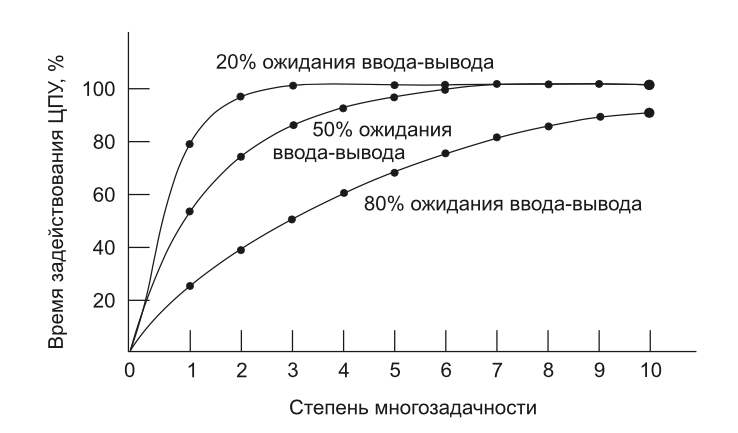
\includegraphics[width=14cm]{lectures/L9/power-of.png}
  \caption{Зависимость загрузки ЦП от степени многозадачности.}
\end{figure}
Процессы ожидают, в основном, выполнение системных вызовов, которые по сути являются запросами к ОС на выполнение привилегированных операций. Это необходимо, так как ОС исполняется в привилегированном режиме с доступом ко всему оборудованию, в отличие от пользовательских процессов. Выполнение системного вызова происходит следующим образом:
\begin{enumerate}[nosep]
  \item Прерывание
  \item передача управления ос
  \item проверка привилегий
  \item работа с оборудованием
  \item загрузка данных для программы
  \item возврат управления
\end{enumerate}
Системный вызов ввода-вывода несколько сложнее. Например, запись на жесткий диск с помощью Си-функции \verb|write| происходит следующим образом:
\begin{enumerate}[nosep]
  \item Прерывание
  \item передача управления ос
  \item проверка привилегий
  \item работа с оборудованием
  \item установка обработчика прерывания
  \item context switch
  \item ...
  \item context switch
  \item загрузка данных для программы
  \item возврат управления исходному процессу
\end{enumerate}
После того, как работа с оборудованием завершена, происходит context switch и исполняется другой процесс до тех пор, пока не сработает прерывание контроллера диска. После этого управление возвращается к исходному процессу.

Простой tcp-сервер приблизительно выглядит так:
\begin{minted}{perl}
while (1) {
    accept
    fork
        read
        write
        read
        write
        ...
        close
        exit
}
\end{minted}
Производительность современных процессоров настолько велика, что время ожидания выполнения read и write значительно превосходит время, затраченное на выполнение остальных операций. Казалось бы, если ожидание ввода-вывода составляет 99.99\% времени исполнения каждого процесса, то можно было бы запустить около 10000 процессов и загрузка ЦП составила бы около 63\%. На практике это не так и эта проблема носит название <<проблема 10000 соединений>>: главным препятствием становится ограничение на размер оперативной памяти, а также необходимость огромного числа переключений контекста.

\subsection{Блокирующие и неблокирующие операции ввода-вывода}
Обычная блокирующая операция ввода-вывода выглядит так:
\begin{minted}{perl}
read(...) -> SUCCESS
read(...) -> FATAL ERROR
\end{minted}
В результате выполнения операции либо успех, либо неудача.

Неблокирующие операции ввода вывода несколько отличаются:
\begin{minted}{perl}
read(...) -> SUCCESS
read(...) -> TEMPORARY ERROR
read(...) -> FATAL ERROR
\end{minted}
Может либо сразу возвращен успех или неудача, а также может быть возращена временная ошибка. Временная ошибка значит, что данная операция временно невозможна.

Это дает возможность писать приложение, работающее на одном ядре, в один процесс, но которое сможет обрабатывать множество различных дескрипторов:
\begin{minted}{perl}
while (1) {
    for my $fh (@fds) {
        my $res = read($fh, ...);
        if ($res) {
            # do work
        }
        elsif ($! ~~ FATAL_ERROR) { # pseudocode
            # close fh, remove from @fds
        }
        else {
            # wait
        }
    }
}
\end{minted}
Это бесконечный цикл, а значит будет расходовать все процессорное время, но это уже некоторое решение, позволяющее обрабатывать большое количество дескрипторов в одном процессе. Соответственно, чтобы избежать загрузки ЦПУ из-за неэффективности цикла был придуман вызов \textbf{select}, который доступен практически в любом языке программирования с доступом к ОС. В вызове select передается вектор сокетов для чтения, вектор дескрипторов для записи и вектор дескрипторов для отслеживания ошибок:
\begin{minted}{perl}
($found,$timeleft) =
    select(
        $readable, # vec
        $writable, # vec
        $errors,   # vec
        $timeout   # in fractional seconds
    )
\end{minted}
Функция vec проставляет конкретный бит или набор бит в строке:
\begin{minted}{perl}
vec($readable, fileno(STDIN),  1) = 1;
vec($readable, fileno(STDOUT), 1) = 1;
vec($readable, fileno(STDERR), 1) = 1;

say unpack "B*", $readable; # 00000111
\end{minted}
Функция \verb|select| возвращает количество готовых дескрипторов и какое время осталось до окончания таймаута.

\section{Интерфейс IO::Select}
Существует интерфейс \verb|IO::Select|, который позволяет удобно работать все с той же функцией \verb|select|:
\begin{minted}{perl}
use IO::Select;

$s = IO::Select->new();

$s->add(\*STDIN);
$s->add($fd);

@ready = $s->can_read($timeout);
\end{minted}
В данном коде показано, как добавлять и удалять дескриптор. На данном этапе уже можно написать нечто более сложное, так как уже можно принимать соединения, добавлять их в select, смотреть, какие готовы, и обрабатывать их. Но существует проблема, что reed, write и т.д являются блокирующими вызовами.

В POSIX был введён флаг \verb|O_NONBLOCK| для \textbf{Fcntl}:
\begin{minted}{perl}
use Fcntl qw(F_GETFL F_SETFL O_NONBLOCK);

$flags = fcntl($fd, F_GETFL, 0)
    or die "Can't get flags for the socket: $!\n";

$flags = fcntl($fd, F_SETFL, $flags | O_NONBLOCK)
    or die "Can't set flags for the socket: $!\n";
\end{minted}
Если применить его на дескриптор, то на этом дескрипторе будет запрещено выполнять блокирующие операции. Любое обращение на этом дескрипторе не заблокируются, а выстовят одну из следующих ошибок:
\begin{itemize}
  \item \textbf{EAGAIN} --- <<попробуй позже>>, штатный ответ, что сокет не готов к запрошенной операции. Это значит, что данный сокет нужно положить в  select на готовность к этой операции.
  \item \textbf{EWOULDBLOCK} --- то же, что и EAGAIN (в большинстве ОС). EWOULDBLOCK значит, что <<если это сделать, то сокет бы заблокировался>>.
  \item \textbf{EINTR} --- <<выполнение системного вызова было прервано прерыванием>>. В этом случае вызов нужно просто повторить.
\end{itemize}
Например, чтение из сокета принимает вид:
\begin{minted}{perl}
use Errno qw(EAGAIN EINTR EWOULDBLOCK);

my $read = sysread($fd, my $buf, SOMELENGTH);

if ($read) { # read >= 0
    # work with data in buf
}
elsif (defined $read) { # read == 0
    # socket was closed
}
elsif ( $! ~~ [ EAGAIN, EINTR, EWOULDBLOCK ] ) {
    # socket not ready for reading
}
else {
    # socket was closed with error $!
}
\end{minted}
Следует отметить, что при блокирующих вызовах sysread считывает нужную длину строки, а при неблокирующих --- считывает столько, сколько может считать.

\section{Цикл событий}
Можно использовать упрощенную схему (описана не очень правильно, но для примера подойдет):
\begin{minted}{perl}
use IO::Select; my $s = IO::Select->new();

my $timeout = 1;
# prepare program...

while () {
    my @ready = $s->can_read($timeout);
    for (@ready) { # do reads }

    my @ready = $s->can_write($timeout);
    for (@ready) { # do writes }
}
\end{minted}
В программе создается один глобальный Select и задается timeout для цикла. После этого запускается так называемый \verb|Event loop|, внутри которого происходят операции ввода-вывода. Создание сокетов происходит на этапе подготовки. Например, в случае сервера нужно создать слушающий сокет и записать его в select.

Удобнее пользоваться замыканиями:
\begin{minted}{perl}
{
    my `$var` = rand();

    my $sub = sub {
        print `$var`;
    }
}
\end{minted}
Замыкания предоставляют возможность сослаться из области видимости некой функции, расположенной ниже, на переменную, объявленную в scope выше:
\begin{minted}{perl}
{
    my `$var` = rand(); # .42;
    my $sub = sub {
        # my $var = .42;
        print `$var`;
    }
}
\end{minted}
Можно сделать генератор функций:
\begin{minted}{perl}
sub decorator {
    my $decor = shift;
    return sub {
        return $decor."@_".$decor;
    }
}

my $dq = decorator "'";
my $dd = decorator '"';
my $ds = decorator '/';

say $dq->('test');  # 'test'
say $dd->('test');  # "test"
say $ds->('test');  # /test/
\end{minted}
В данном примере возвращается функция, которая замыкает переданный при генерации параметр, и добавляет к своему строковому аргументу его слева и справа.

Ещё один пример, набор функций, в которых прибавляется значение к своему аргументу:
\begin{minted}{perl}
my @subs;

for my $var (1..10) {
    my $sub = sub {
        return $var + $_[0];
    };
    push @subs, $sub;
}

for my $sub (@subs) {
    say $sub->(2);
}
# 3 4 5 6 7 8 9 10 11 12

for my $sub (@subs) {
    say $sub->(10);
}
# 11 12 13 14 15 16 17 18 19 20
\end{minted}

Это позволяет замыкать дескриптор внутри некоторой функции (называется callback):
\begin{minted}{perl}
my $fd = socket...
wait_socket_readable($fd, sub {
    read($fd, ...)
})

# ...

our %waiters;
sub wait_socket_readable {
    my ($fd,$cb) = @_;
    $select->add($fd);
    push @{ $waiters{$fd} }, $cb;
}
# Event loop:
while () {
    # ...
    for my $fd (@ready) {
        for my $cb ( @{ $waiters{$fd} } ) {
            $cb->();
        }
    }
}
\end{minted}
Так как эта функция сразу не готова вернуть результат, она передается функции \verb|wait_socket_readable|, которая добавляет сокет в \verb|select|, а ссылку на функцию в специальный хеш. После этого внутри event loop для всех готовых дескрипторов вызываются функции, которые ждали их готовности.

Это позволяет нам писать последовательные цепочки кода:
\begin{minted}{perl}
my $fd = socket...

wait_socket_readable($fd, sub {
    sysread($fd, ...);

    wait_socket_writable($fd, sub {
        syswrite($fd, ...);

        wait_socket_readable($fd, sub {
            sysread($fd, ...);

            # ...
        });
    });
});

# ...
        my @wait = @{ $waiters{$fd} };
        @{ $waiters{$fd} } = ();
        for my $cb ( @wait ) {
\end{minted}

Также может потребоваться ограничить время ожидания сокета, например секундой. Для этого можно сделать функцию, которая представляет собой таймер:
\begin{minted}{perl}
wait_timeout 1, sub { ... };

our @deadlines;
sub wait_timeout {
    my ($t,$cb) = @_;
    my $deadline = time + $t;
    @deadlines =
        sort { $a->[0] <=> $b->[0] }
        @deadlines, [ $deadline, $cb ];
}

# Event loop:
while () {
    #...
    while ($deadlines[0][0] <= time) {
        my $next = shift(@deadlines);
        my $cb = $next->[1];
        $cb->();
    }
}
\end{minted}
В event loop, помимо работы с сокетами, содержится цикл по deadline.

В этом примере применен довольно примитивный подход (для примера): здесь просто применен sort на каждую операцию, что плохо, так как есть гораздо более адекватные алгоритмы вставки элемента в массив.

Здесь есть одна опасность. Пусть дан следующий код:
\begin{minted}{perl}
wait_timeout 1, sub {
    wait_timeout 0, sub {
        wait_timeout 0, sub {
            wait_timeout 0, sub {
                wait_timeout 0, sub {
                    wait_timeout 0, sub {
                        wait_timeout 0, sub {
                            ...
                        };
                    };
                };
            };
        };
    };
};
\end{minted}
Его можно свернуть до такого кода:
\begin{minted}{perl}
wait_timeout 1, sub {
    my $sub; $sub = sub {
        wait_timeout 0, $sub;
    }; $sub->();
};
\end{minted}
В event loop вызывается callback для первого элемента массива deadlines и этот элемент удаляется из массива:
\begin{minted}{perl}
my $deadline = time + $t;
unshift @deadlines, [$deadline, $cb];
# ...
    while ($deadlines[0][0] <= time) {
        my $next = shift(@deadlines);
        my $cb = $next->[1];
        $cb->();
    }
\end{minted}
Но при исполнении callback'а в массив deadlines добавляется очередной элемент. Получается зацикливание. Это нехорошо, таймеры не должны себя так вести.

Поэтому необходимо сделать следующее:
\begin{itemize}
  \item Необходимо зафиксировать время (сохранить в переменную \verb|$now|) и пока идет выполнение цикла эта переменная не должна меняться.
  \item Внутри цикла все расчеты, сравнения и так далее должны выполняться относительно этого фиксированного времени.
  \item Чтобы избежать зацикливания, event loop необходимо переписать: сначала извлечь все таймеры, для которых нужно выполнить callback, а затем выполнить соответствующие callback'и. В ходе выполнения callback'ов массив \verb|@deadlines| может пополниться, но это уже не будет влиять на исполнение цикла.
\end{itemize}
Получается следующий код:
\begin{minted}{perl}
our `$now`;
our @deadlines;

sub wait_timeout {
    my ($t,$cb) = @_;
    my $deadline = `$now` + $t;
    @deadlines =
        sort { $a->[0] <=> $b->[0] }
        @deadlines, [ $deadline, $cb ];
}
# Event loop:
while () {
    `$now` = time;
    #...
    my @exec;
    push @exec, shift @deadlines
        while ($deadlines[0][0] <= `$now`);
    for my $dl (@exec) {
        $dl->[1]->();
    }
}
\end{minted}

\section{Обобщенный интерфейс}
Предыдущие рассуждения приводят к некому обобщённому интерфейсу:
\begin{minted}{perl}
io( $fd, READ | WRITE, $cb);
timer( $timeout, $cb );
runloop();
\end{minted}
Есть функция io, которая принимает дескриптор, требуемое действие и callback. Также есть возможность задать таймер на какое-то время. Функция runloop(); вызывается один раз и запускает основной цикл.

Если до запуска основного цикла не были установлены никакие ожидания ввода/вывода и не были установлены таймеры, этот цикл представляет собой бесконечный цикл, в который никак невозможно войти. Поэтому во многих реализациях event loop он реализован таким образом, что в такого рода ситуации просто выходит.

Для perl была написана библиотека AnyEvent, которая представляет такую абстракцию (обобщенный интерфейс) поверх совершенно различных реализаций событийных циклов. Здесь стоит отметить, что одновременно использовать два событийных цикла нельзя: функция запуска цикла является блокирующей. AnyEvent позволяет писать программу, не задумываясь о реализации конкретно используемого событийного цикла, используя следующий интерфейс:
\begin{minted}{perl}
AE::io( $fd, $flag, $cb );
AE::timer( $after, $interval, $cb );
AE::signal( $signame, $cb );
AE::idle( $cb );
AE::now();
\end{minted}
Часто используется событийный цикл AnyEvent::loop, написанный на чистом perl с использованием select.

\section{Модуль AnyEvent}
\subsection{Интерфейс AE::io}%38 31:32
В AE::io есть два интерфейса:
\begin{itemize}
\item \textbf{объектный}: вызывается метод io объекта AnyEvent:
\begin{minted}{perl}
AnyEvent->io( fd=>\*STDIN, poll=>'r',
    cb => sub {
        my $line = <STDIN>;
        AnyEvent->io( fd=>\*STDOUT, poll=>'w',
            cb => sub {
                print $line;
            }
        );
    }
);
\end{minted}
\item \textbf{сокращённый}: вызывается функция, которой передаются 3 аргумента:
\begin{minted}{perl}
AE::io \*STDIN, 0, sub {
    # stdin is readable;
    my $line = <STDIN>;
    AE::io \*STDOUT, 1, sub {
        # stdout is writable
        print $line;
    };
};
\end{minted}
\end{itemize}
Сокращенный интерфейс чуть-чуть быстрее и компактнее выглядит, поэтому примеры будут приведены именно используя сокращенный интерфейс.
% TODO Про использование  функциями класса SYS

В приведенном примере есть одна проблема: блок, который выполняется, если STDOUT готов к записи будет выполняться бесконечно. Чтобы решить эту проблему можно использовать модуль Guard:
\begin{minted}{perl}
my $guard = guard { # same as guard(sub { ... })
    say '$guard was unrefed';
};
say "Before...";
undef $guard;
say "After";
\end{minted}
Функция guard принимает в качестве параметра блок кода и возвращает переменную. Блок кода исполняется тогда, когда переменная, которую он вернул, будет уничтожена:
\begin{minted}{perl}
Before...
$guard was unrefed
After
\end{minted}
Сделать Guard очень просто. Следующей реализации достаточно, чтобы заработал предыдущий пример (метод cancel позволяет отменить guard):
\begin{minted}{perl}
sub Guard::DESTROY {
    my $self = shift;
    $self->[0]->() if $self->[0];
}

sub Guard::cancel {
    $_[0][0] = undef;
}

sub guard(&) {
    my $cb = shift;
    bless [$cb], 'Guard';
}
\end{minted}
Сам модуль Guard написан на XS и устроен несколько сложнее.

Модуль Guard используется следующим образом. Некоторое отложенное действие \verb|delayed_action| возвращает guard:
\begin{minted}{perl}
use Guard;

sub delayed_action {
    my ($smth,$cb) = @_;
    my $state = ...

    # ...

    return guard {
        cancel_action($state);
    }
}


my $w = delayed_action(..., sub { ... });
#  $w is a guard
# ...
undef $w; # cancels action
\end{minted}
Если по ходу программы оказывается, что не нужно дожидаться вызова callback'а, достаточно вызвать undef на guard, после чего вызывается \verb|cancel_action|, которая отменяет отложенное действие.

В приложении к AE, нужен объект, который вызовет callback после своего уничтожения:
\begin{minted}{perl}
my ($r,$w);

$r = AE::io \*STDIN, 0, sub {
    # stdin is readable;
    my $line = <STDIN>;

    $w = AE::io \*STDOUT, 1, sub {
        # stdout is writable
        print $line;

        undef $w; # not interesting
                  # in write anymore
    };
};

AE::cv->recv; # Run loop
\end{minted}
Все вызовы AnyEvent'а возвращают guard'ы, поэтому если он не был сохранен, он сразу же уничтожается и отменяет callback.

Таймер реализуется аналогично. Функция AE::timer имеет два аргумента, время до срабатывания таймера и периодичность вызова таймера:
\begin{minted}{perl}
my $w; $w = AE::timer 1, 0, sub {
    undef $w;
    say "Fired after 1s";
};

my $p; $p = AE::timer 0, 0.1, sub {
    state $counter = 0;
    return undef $p if ++$counter > 5;
    say "Fired $counter time";
};

AE::cv->recv; # Run loop
\end{minted}
Если нам не нужен периодический таймер, то в качестве второго аргумента нужно передать нулевое значение. Следует отметить, что, для того, чтобы переменная \verb|$w| была видна внутри блока, ее сначала нужно объявить. После этого она станет видна внутри блока и ей уже можно присвоить значение. Про утечки памяти и замыкания будет отдельно рассказано на последней лекции, поэтому сейчас этот вопрос обсуждаться не будет.

В большинстве практических случаях использования io и таймеров достаточно, чтобы написать любую сетевую программу: написать сервер, подключиться куда-нибудь и что-либо сделать.

Также в AE есть обработка сигналов. Например, в консольных приложениях можно обработать сигнал INT (ctrl+C):
\begin{minted}{perl}
my $s;$s = AE::signal INT => sub {
    warn "Received SIGINT, exiting...\n";
    exit(0);
};

AE::cv->recv; # Run loop
\end{minted}
Также доступны AE::idle и AE::now (зафиксированное время, как это обсуждалось ранее):
\begin{minted}{perl}
my $i = AE::idle sub {
    printf "now: %f, idle...\n",AE::now();
};
\end{minted}
AE::idle дает возможность установить callback, который вызывается в случае, если вызывать больше нечего:
\begin{minted}{perl}
while () {
    $now = time;

    if (@ready) {
        # ...
    }
    elsif(@timers) {
        # ...
    }
    else {
        call_idle();
    }
}
\end{minted}
AE::idle может понадобиться, если на довольно сильно загруженный сервере иногда нужно выполнять не очень важный код.

%\begin{figure}[H]
  %\includesvg[width=\textwidth]{Technosfera-perl-master/lectures/async/123}
%\end{figure}

При разработке следует использовать AE, а не какой-то конкретный событийный цикл, поскольку:
\begin{itemize}
	\item На основе AE::io и AE::timer был создан модуль AE::Handle, который предоставляет более удобный способ чтения и записи в файл.
	\item Внутри AE::Handle реализован модуль AE::TLS, который обеспечивает возможность поддерживать TLS-соединения.
	\item Поверх AE::io, AE::timer и AE::Handle сделан AE::Socket, который позволяет создавать сервер и клиент.
	\item Поверх AE::Socket создано огромное количество модулей, в том числе AE::HTTP-Server.
\end{itemize}


\subsection{AE:cv (condvar)} %47 43:43
В AE есть модуль condition variable, для которого есть как короткий синтаксис (AE:cv), так и длинный (AE::condvar):
\begin{minted}{perl}
my $cv = AE::cv(); # create condvar

my $p; $p = AE::timer 0, 0.1, sub {
    state $counter = 0;
    if (++$counter > 5) {
        undef $p;
        $cv->send;
        return;
    };
    say "Fired $counter time";
};

$cv->recv;
\end{minted}
У объекта \verb|$cv| есть два метода, send и recv. Если вызвать recv, то он блокируется до тех пор, пока не будет вызван send. Примерная реализация выглядит следующим образом:
\begin{minted}{perl}
my $cv = bless {}, 'condvar';

sub condvar::recv {
    my $self = shift;

    $self->_one_loop
        while !$self->{sent};

    return @{ $self->{args} };
}

sub condvar::send {
    my $self = shift;

    $self->{sent} = 1;

    $self->{args} = [ @_ ];
}
\end{minted}
Внутри есть функция \verb|_one_loop|, которая делает один проход событийного цикла. Метод recv выполняет эту функцию до тех пор, пока не будет вызван метод send, после чего возвращает то, что было передано через send.

У AE::cv есть еще дополнительное применение --- вызовы begin и end, что необходимо, чтобы делать программы псевдопараллельными:
\begin{minted}{perl}
my $cv = AE::cv;

$cv->begin;
my $w1;$w1 = AE::timer rand(),0, sub {
    undef $w1;
    say "First done";
    $cv->end;
};

$cv->begin;
my $w2;$w2 = AE::timer rand(),0, sub {
    undef $w2;
    say "Second done";
    $cv->end;
};

$cv->recv;
\end{minted}
При этом вызовы begin и end устроены следующим образом:
\begin{minted}{perl}
sub condvar::begin {
    my $self = shift;
    $self->{counter}++;
}

sub condvar::end {
    my $self = shift;

    $self->{counter}--;

    if ($self->{counter} == 0) {
        $self->send();
    }
}
\end{minted}
Также существует возможность установить callback, как при создании condvar:
\begin{minted}{perl}
my $cv = AE::cv {
   say "cv done"
};

$cv->begin;
my $w1;$w1 = AE::timer rand(),0, sub {
    undef $w1;
    say "First done";
    $cv->end;
};
$cv->begin;
my $w2;$w2 = AE::timer rand(),0, sub {
    undef $w2;
    say "Second done";
    $cv->end;
};

$cv->recv;
\end{minted}
так и где-нибудь после исполнения передать в функцию \verb|cb|:
\begin{minted}{perl}
my $cv = AE::cv;

$cv->begin;
my $w1;$w1 = AE::timer rand(),0, sub {
    undef $w1;
    say "First done";
    $cv->end;
};
$cv->begin;
my $w2;$w2 = AE::timer rand(),0, sub {
    undef $w2;
    say "Second done";
    $cv->end;
};

$cv->cb(sub {
   say "cv done";
});
$cv->recv;
\end{minted}
Эти две записи эквивалентны. Собственно, cb реализуется следующим образом:
\begin{minted}{perl}
sub AE::cv(;&) {
    my $self = bless {}, 'condvar';
    $self->{cb} = shift;
    return $self;
}

sub condvar::cb {
    my $self = shift;
    $self->{cb} = shift;
}

sub condvar::send {
    my $self = shift;

    $self->{sent} = 1;

    $self->{args} = [ @_ ];

    if ($self->{cb}) { $self->{cb}->() };
}
\end{minted}

\subsection{Применение AE:cv}
Для примера будет использоваться простая асинхронная функция, например случайный таймер:
\begin{minted}{perl}
sub async {
    my $cb = pop;

    my $w;$w = AE::timer rand(0.1),0,sub {
        undef $w;

        $cb->();
    };

    return;
}
\end{minted}

Можно использовать AE:cv для параллельного исполнения кода. Например, данный код скачивает данные по url из массива:
\begin{minted}{perl}
my $cv = AE::cv;
my @array = 1..10;

for my $cur (@array) {
    say "Process $array[$cur]";
    $cv->begin;
    async sub {
        say "Processed $array[$cur]";
        $cv->end;
    };
}

$cv->recv;
\end{minted}
Эта программа работает замечательно, пока размер массива не очень большой. Попытка запустить 10000 паралелльных задач обычно ни к чему хорошему не приводит. Поэтому необходимо использовать параллельное исполнение с ограничениями, о чем будет сказано позднее.

Если не известно, что массив не является пустым, необходимо всегда вызывать \verb|$cv->begin;| после создания cv, а \verb|$cv->end| перед \verb|$cv->recv|:
\begin{minted}{perl}
my $cv = AE::cv; $cv->begin;
my @array = 1..10;

for my $cur (@array) {
    say "Process $array[$cur]";
    $cv->begin;
    async sub {
        say "Processed $array[$cur]";
        $cv->end;
    };
}

$cv->end; $cv->recv;
\end{minted}
Последовательное исполнение можно получить следующим образом:
\begin{minted}{perl}
my $cv = AE::cv;
my @array = 1..10;

my $i = 0;
my $next; $next = sub {
    my $cur = $i++;
    return if $cur > $#array;
    say "Process $array[$cur]";
    async sub {
        say "Processed $array[$cur]";
        $next->();
    };
}; $next->();

$cv->recv;
\end{minted}

Параллельное исполнение с ограничением можно получить, если вызвать next несколько раз, что породит несколько логических нитей исполнения:
\begin{minted}{perl}
my $cv = AE::cv;
my @array = 1..10;

my $i = 0;
my $next; $next = sub {
    my $cur = $i++;
    return if $cur > $#array;
    say "Process $array[$cur]";
    async sub {
        say "Processed $array[$cur]";
        $next->();
    };
}; $next->();

$cv->recv;
\end{minted}
Если неизвестно, будет ли массив пустым, нужно модифицировать код по аналогии:
\begin{minted}{perl}
my $cv = AE::cv; `$cv->begin`;
my @array = 1..10;

my $i = 0;
my $next; $next = sub {
    my $cur = $i++;
    return if $cur > $#array;
    say "Process $array[$cur]";
    $cv->begin;
    async sub {
        say "Processed $array[$cur]";
        $next->();
        $cv->end;
    };
}; $next->() for `1..5`;

`$cv->end`; $cv->recv;
\end{minted}

\section{Coro}
Модуль Coro позволяет реализовать кооперативную многозадачность, то есть когда функции делят время в рамках одного процесса:
\begin{minted}{perl}
use Coro;

async { # create new stack
    say 2;
    cede; #
    say 4;
};

say 1;
cede;
print 3;
cede;

# 1 2 3 4
\end{minted}
AnyEvent тоже реализует кооперативную многозадачность, но там каждая логическая нить исполнения не обладает собственным стеком.

AnyEvent имеет следующие особенности:
\begin{itemize}
  \item[-] нет стека
  \item[~] линейный код неудобен
  \item[+] параллельный код легко
  \item[+] стек нити не ограничен
  \item[+] дедлок невозможен
\end{itemize}

Coro имеет следующие особенности:
\begin{itemize}
  \item[+] есть стек
  \item[+] линейный код удобен
  \item[-] параллельный неудобно
  \item[-] стек ограничен
  \item[-] возможен дедлок
\end{itemize}

%\setcounter{chapter}{9}
\chapter{Ускоряем perl. Расширяем «C».}
\section{Генерация XS модулей}
Чтобы сгенерировать XS модуль, необходимо знать каким образом был скомпилирован perl. Все XS модули должны быть скомпилированы также. Узнать это можно с помощью вызова:
\begin{minted}{bash}
% perl -V:make
make='dmake';
\end{minted}
В данном случае perl был скомпилирован для операционной системы windows с помощью dmake.

Утилита h2xs, которая идет в дистрибутиве perl, позволяет генерировать XS-интерфейс к коду на C. Параметр -b позволяет указывать минимальную версию perl, на которой предполагается запускать модуль, для целей обеспечения обратной совместимости. При этом, чем ниже указанная версия, тем больше <<обвязки>> будет строиться вокруг кода на C. Ключ -n позволяет указать используемый namespace, то есть полный путь к вашему пакету.

Если работающего кода пока нет, создать необходимый каркас для будущего модуля можно с помощью вызова:
\begin{minted}{bash}
% h2xs -b 5.10.1 -n local::sferamail::perlxs
\end{minted}
Будет создана директория со всеми нужными файлами для компиляции XS-модуля. Этот каркас можно было бы создать вручную, но так как требования к коду меняются от версии к версии, лучше всего это делать в автоматическом режиме. Если внутри данного каталога запустить утилиту make, скомпилируется пока пустой модуль.

Если программа на C уже написана, то сгенерировать XS-интерфейс можно указав путь к header-файлу с помощью той же утилиты:
\begin{minted}{bash}
h2xs -n local::sferamail::locale -O -x "F:\locale.h"
\end{minted}
В результате будет создана привязка к указанной библиотеке на C. Также можно будет сразу скопилировать XS модуль, после чего функции из библиотеки можно будет вызывать из perl. Базовый набор файлов, необходимых для создания модуля следующий:
\begin{description}[nosep, labelindent=2mm]
  \item[/ppport.h]--- файл, необходимый для обратной совместимости с другими версиями perl.
  \item[/lib/local/sferamail/perlxs.pm]--- файл, который нужно будет подключить в основной программе.
  \item[/perlxs.xs]--- файл, содержащий код XS модуля.
  \item[/fallback/const-c.inc и /fallback/const-xs.inc]: константы необходимые для работы в установленной версии perl. Эти файлы генерируются автоматически.
  \item[/Makefile.PL] Этот файл нужно исполнить на интерпретаторе perl, чтобы он создал обычный makefile и набор заголовочных файлов, которые совместимы с установленной версией perl.
  \item[/README]--- описание модуля
  \item[/t/local-sferamail-perlxs.t]--- тесты (опц.)
  \item[/Changes]--- история версий модуля
  \item[/MANIFEST]--- файл, содержащий список файлов в пакете.
\end{description} \noindent
Сборка и тестирование модуля выполняются с помощью команд:
\begin{minted}{bash}
% perl Makefile.PL
% dmake
% dmake test

t/sferamail-perlxs.t .. ok
All tests successful.
Files=1, Tests=1,  0 wallclock secs ( 0.00 usr +  0.08 sys =  0.08 CPU)
Result: PASS

% dmake install
\end{minted}
После этого скомпилированный модуль может быть использован.




\section{Макропроцессор}
На самом деле, код XS модуля отличается от привычного кода на C. На самом деле, XS является макро-языком для perl.
\begin{figure}[H] \centering
  \begin{tikzpicture}[
        entity/.style={ minimum height=1cm, minimum width=2.5cm, draw } ]
    \draw node[entity                      ] (XSU) {XSUBPP}
          node[entity,   right    = of XSU ] (C)   {C-File}
          node[entity,   below    = of C   ] (PM)  {PM-file}
          node[entity, below left = of XSU ] (XS)  {XS-file}
          node[entity, above left = of XSU ] (TM)  {TYPEMAP};
    \begin{scope}[line width = 1.2pt]
      \draw[-stealth] (PM) -- (C);
      \draw (C) -- (XSU) --+ (-2,0) edge (TM) edge (XS);
    \end{scope}
  \end{tikzpicture}
\end{figure} \noindent
А именно макрокомпилятору XSUBPP на вход подается XS-файл и TYPEMAP, то есть правила преобразования типов данных между C и perl, а в результате его выполнения макрокоманды расворачиваются в код на C. Именно этот получившийся файл компилируется компилятором языка C в файл с расширением so. Доступ к функциям из этого файла можно получить используя полученный ранее файл с расширением pm.

\section{Типы данных}
\subsection{Основные типы переменных}
Доступ к переменным perl из кода на C представляет из себя сложную задачу. Именно поэтому был создан макроязык XS, который позволяет приводить типы и работать со структурами данных perl. Однако понимать, как устроены структуры данных в perl необходимо, в том числе, и для целей отладки.

В perl существую следующие типы переменных:
\begin{itemize}[nosep]
  \item \textbf{SV}: Scalar Value
  \begin{itemize}[nosep]
    \item \textbf{IV}: signed integer value
    \item \textbf{UV}: unsigned integer value
    \item \textbf{NV}: double
    \item \textbf{PV}: pointer value
    \item \textbf{SV}
  \end{itemize}
  \item \textbf{AV}: Array Value
  \item \textbf{HV}: Hash Value
\end{itemize}
эти типы имеют одну и ту же структуру header'а, который представляет собой структуру из 4 значений:
\begin{figure}[H] \centering
\begin{tikzpicture}
\begin{simpleblock}[shift={(0,0)}]
	\add[color=blue!12, point]{ANY};
    \draw[line width=1pt, -latex] (R)+(1,0) node[anchor=west]{%
        Ссылка на данные из этой структуры данных}--(R);
	\add{REFCNT};
    \draw[line width=1pt, -latex] (R)+(1,0) node[anchor=west]{%
        Количество ссылок на эту структуру (нужно для работы сборщика мусора)
        }--(R);
	\add[width=0.75*3cm, flags] {FLAGS};
	\add[color=red!12, width=0.25*3cm, font = {\tiny}, toright] {\ TYPE};
	\add[point, color=blue!12] {SV\_U};
    \draw[line width=1pt, -latex] (R)+(1,0) node[anchor=west]{%
       SV\_U}--(R);
\end{simpleblock}
\end{tikzpicture}
\end{figure}\noindent
В FLAGS и TYPE хранится информация, характеризующая эту SV:
\begin{figure}[H] \centering
  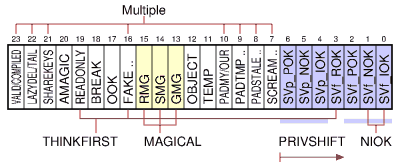
\includegraphics[width=10cm]{lectures/L10/flags.png}
\end{figure}\noindent
Помнить, какой бит флага что обозначает не требуется, так как они меняются от версии к версии perl. Поэтому необходимо использовать только именованные константы.

\subsection{Pointer Value}
Pointer Value (PV) --- одно из самых распространенных использований SV-ек в Perl, предназначенное для хранения строк. SvPV выглядит следующим образом:
\begin{figure}[H] \centering
	\begin{tikzpicture}[sv schemes]

		\begin{scope}[ shift={(-6,0)}, 	sv style=named SV,
			             scale=0.5,			setlabel=firstsv   	]
		    \draw (0,0.35) node {\bf svu\_pv};
		    \coordinate (temp2) at (1.5,3.5);
		\end{scope}

		\fill (firstsv-1) circle (0.7mm) (firstsv-2) circle (0.7mm);

		{ [shift=(temp2), xpv style = named xpv]
			\node {STASH};	 \node {MAGIC};	 \node {cur};	 \node {len};	}

		\draw[connect line] (firstsv-2) -- (xpv-1.west);


		{ [ shift= {($(xpv-1.east)+(4cm,0)$)},
			start chain=stack going right, anchor=west]
			\node [sn] {a}; \node [sn] {b};
			\node [sn] {c}; \node [sn] {};
			\node [sn] {x}; \node [sn] {y};
			\node [sn] {z}; \node [gsn] {\verb|\0|};
			\node [gsn] {}; \node [gsn] {C};     		}



		\draw[connect line] (firstsv-1)  --++ (0.25,0)
		  |- ++ (5.5,2.35) coordinate (temp2)  |- (stack-1.west);
		\draw[connect line, dashed] (temp2) --+ (0,-2.5) coordinate (temp3);

		{ [shift={(temp3)},start chain=hek going right,
			anchor=north east, xshift=-1cm]
			\node [sn wide] {hash};
			\node [sn wide] {len};
			\foreach \l in {s,h,a,r,e,d} \node [ysn] {\l};
			\node [gsn] {\verb|\0|};
			\node [sn wide] {flag};
		}

		\path [setcut=stack-4.center];

		\node [above=of stack-2] {\texttt{char[]}};
		\node [above=of hek-9  ] {\texttt{hek}};

	\end{tikzpicture}
\end{figure}
То есть в параметре \verb|SV_U| будет лежать ссылка на область памяти, где расположена строка, а по ссылке в параметре \verb|ANY| указана специальная структура, в которой хранится текущая длина строки (cur) и максимальная длина строки, для которой уже была выделена память (len). Perl всегда выделяет больше памяти, чем нужно для хранения строковой переменной, чтобы в большинстве случаев не было необходимости выделять дополнительную память при увеличении длины строки. Каждая строка в Perl должна заканчиваться нуль-байтом. Начиная с версии 5.18 в последний байт строки начали складывать количество ссылок на эту строку из перловых программ.


У SvPV есть флаг SvOOK, который обозначает, что у строки обрезано начало. В первом байте строки содержится число, которое указывает сколько байт строки нужно пропустить:
\begin{figure}[H] \centering % SvOOK
	\begin{tikzpicture}[sv schemes]

		\begin{scope}[shift={(-6,0)}, scale=0.5]
			\drawsv\draw (0,0.5) node {ARRAY};\drawsvflagbits
			\coordinate (temp1) at (2,0.5);
			\coordinate (temp2) at (1.5,3.5);
			\node[above] at (1.5,4) {\tt sv};
			\draw (-0.5,1.25) node {\tiny\bf POK, OOK};
		\end{scope}
		\fill (temp1) circle (0.7mm) (temp2) circle (0.7mm);

		{ [shift=(temp2), xpv style= named xpviv]
			\node {STASH};  \node {MAGIC};
			\node {cur}; 	  \node {len};
		}

		%\node[above, xshift=0.5cm, yshift=-0.1cm] at (xpviv-1.north) {\tt xpviv};

		\draw[connect line] (temp2) -- (xpviv-1.west);
		\path (xpviv-1.east)+(1.5cm,0) coordinate (temp3);


		{ [shift= {(temp3)},start chain=stack going right, anchor=west]
			\node [gsn] {2}; \node [gsn] {}; \node [sn] {c};\node [sn] {};
			\node [sn] {x};\node [sn] {y}; \node [sn] {z};
			\node [gsn] {\verb|\0|}; \node [gsn] {};\node [gsn] {};
			\node [above=of stack-9] {\texttt{char[]}};
			\path [setcut=stack-4.center];
		}
		\draw[connect line] (temp1) --++ (0.25,0) |- ++ (4,2.35) -| (stack-2.north east);

	\end{tikzpicture}
\end{figure}

\subsection{MAGIC} % TODO SvPVMG
С помощью флага MAGIC можно создавать переменные, у которых переопределены операции чтения, изменения и так далее. Если созданная SV-ка имеет такой флаг, в ней параметр ANY должен будет указывать на специальную структуру \verb|xpvmg| (см. схему ниже), у которой в свою очередь по ключу MAGIC указана другая структура ---  \verb|magic|. В структуре \verb|magic| содержится ссылка на некоторый объект (другая SV, Array Value и так далее) и должны быть переопределены виртуальные методы GET, SET, LEN и так далее, причем обязательно переопределять только некоторые из них.

\begin{figure}[H] \centering
	\begin{tikzpicture}[sv schemes]
		\begin{scope}[
			shift={(-6,0)}, 	sv style=named SV,
			scale=0.5,			setlabel=firstsv	]
		\end{scope}

		\path [setcircle=firstsv-2];

		{ [shift=(firstsv-2), xpv style=named xpvmg]
			\node[fill=yellow!20] {STASH};
			\node[fill=yellow!20] {MAGIC};
			\node {cur}; 	\node {len};
			\node[fill=gray!30]   {xiv\_u};
			\node[fill=gray!30]   {xnv\_u}; }

		{ [shift={(-4,5)}, xpv style=named magic state]
			\node {mgs\_sv};
			\node {mgs\_flags};
			\node {mgs\_ss\_ix};
		}



		\begin{scope}[shift={($(xpvmg-2)+(1,0)$)}, xpv style=named magic]
			\node[xscale=0.666,minimum width=3cm,text width=2.8cm] {moremagic};
			\node {virtual};
			\node[xscale=0.666,minimum width=3cm,text width=2.8cm] {private};
			\node {len}; \node {obj}; 	\node {ptr};
		\end{scope}
		\draw[line width = 1pt,fill=red!20]
		($(magic-3.south)!0.5!(magic-3.south east)$) rectangle (magic-3.north);
		\node[above,xscale=0.5] at ($(magic-3.south)!0.25!(magic-3.south east)$) {type};
		\node[above,xscale=0.5] at ($(magic-3.south)!0.75!(magic-3.south east)$) {flags};

		\foreach \n in {1,2,5,6} {
			\path (magic-\n.east)+(-0.25,0) coordinate(magic-\n-point);
			\path[setcircle=magic-\n-point];
		}

		\begin{scope}[shift={($(xpvmg-1.east)+(2,-6.95)$)},
			sv style=named hv,scale=0.5,setlabel=temphv]
		\end{scope}

		\begin{scope}[shift={($(magic-6.east)+(1.5,-1.125)$)},
			sv style=named {},scale=0.5,setlabel=tmpsv]
		\end{scope}


		\begin{scope}[shift={($(magic-1-point)+(1,4)$)}, xpv style=named magic,
			hack/.style={xscale=0.666,minimum width=3cm,text width=2.8cm}]
			\node[hack]{moremagic};\node{virtual};\node[hack]{private};
			\node{len};\node{obj};\node{ptr};
		\end{scope}
		\draw[line width = 1pt,fill=red!20] ($(magic-3.south)!0.5!(magic-3.south east)$) rectangle (magic-3.north);
		\path (magic-1.east)+(-0.25,0) coordinate(magic2-1-point)
		(magic-1.west) coordinate(magic2-1-west);

		\begin{scope}[
			shift={($(magic2-1-point)+(1,0)$)}, xpv style=named magic,
			hack/.style={xscale=0.666,minimum width=3cm,text width=2.8cm}]
			\node[hack]{moremagic};\node{virtual};\node[hack]{private};
			\node{len};\node{obj};\node{ptr};
		\end{scope}

		\draw[line width = 1pt,fill=red!20]
			($(magic-3.south)!0.5!(magic-3.south east)$) rectangle (magic-3.north);
		\path (magic-1.east)+(-0.25,0) coordinate (magic3-1-point);

		{ [	shift= {($(magic-2-point)+(2,0)$)},
			start chain=stack going right, anchor=west]
			\foreach \t in {GET,SET,LEN,CLEAR,FREE,COPY,DUP,LOCAL}
			{ \node[sn, minimum height=0.8cm, align=center] {\tiny \t\\ };
			  \path[yshift={1.2ex},setcircle=\tikzchaincurrent]; } 			}
		\node [above=of stack-8] {\texttt{mgvbl}};



		\begin{scope}[connect line]
			\foreach[count=\n] \l in { get,set,len }
				\draw (stack-\n.center) --+ (0,-1.6+0.3*\n)
				 node[right, xshift=-0.27cm,yshift=-0.18cm]{\texttt{\&magic\_\l}};
			\draw ($(magic state-1.east)+(-0.5,0)$)
				coordinate (magstate) --+ (1, 0) |- (-7.5,3) |- (-7,1.75);
			\draw (magic-1-point) --+ (1, 0)  |- (magic2-1-west);
			\draw (magic-2-point) --+ (2, 0);
			\draw (magic2-1-point) -- (magic-1.west);
			\draw (magic-5-point) --+ (0.75, 0);
			\draw (temphv-2) --+ (1, 0);
			\draw (firstsv-2) -- (xpvmg-1.west);
			\draw (xpvmg-2.east)  + (-0.5,0 ) --+ (1, 0);
			\draw (xpvmg-1.east)-|++( 0.4,-5) --++ (0.6,0);
		\end{scope}



		\path[setcircle=temphv-2,setcircle=magic2-1-point,setcircle=magic3-1-point,setcircle=magstate];
	\end{tikzpicture}
\end{figure}
Таким образом реализован модуль \verb|Tie::Hash|, который позволяет изменять поведение хэша (делать его <<тайным>>). Для этого программист должен написать свои собственные функции, которые определяют его поведение. Например при записи значения в хэш сделать так, чтобы реально происходила запись в файл, и так далее. Например, на основе этого работает модуль для удобного доступа к содержимому BDB-файла (файл базы данных Berkeley DB, которая хранить данные в виде <<ключ--значение>> в файле на жестком диске). А именно: получая или изменяя значения хэша фактически будут работой с BDB-файлом.

\subsection{Ссылка на переменную}
Reference Value (RV) --- ссылка на Scalar Value. Ссылка на переменную выглядит очень просто: создается header, у которого в последнем поле находится ссылка на SV. Больше никаких дополнительных структур не создается и память не выделяется.

\begin{figure}[H]\centering  % SvRV
\begin{tikzpicture}[sv schemes]
	\begin{scope}[
		shift={(-4,0)}, 	sv style=named SV,
		scale=0.5,			setlabel=firstsv
	]  \draw (0,0.35) node {\bf svu\_rv};
	\end{scope}

	\begin{scope}[
		shift={(0,-0.05)},	sv style=named SV,
		scale=0.5,			setlabel=secondsv
	]\end{scope}

\draw[connect line, setcircle=firstsv-1 ]
	(firstsv-1)  --+ (1,0) |- (secondsv-3);
\draw[connect line, setcircle=secondsv-2]
	(secondsv-2) --+ (1,0);

\end{tikzpicture}
\end{figure}

\subsection{Массив и Хэш}
Array Value --- массив в perl, в header'е в последнем поле находится ссылка на начало массива, а в первом поле --- на структуру \verb|xpvav|.

\begin{figure}[H] \centering
\begin{tikzpicture}[sv schemes]
	\begin{scope}[
		shift={(-6,0)}, 	sv style=named AV,
		scale=0.5,			setlabel=firstsv
	]  \draw (0,0.5) node {ARRAY} (-0.5,1.5) node {FLAGS};
	\end{scope}

\path [setcircle=firstsv-1, setcircle=firstsv-2];

{ [shift=(firstsv-2), xpv style=named xpvav]
 \node {STASH}; \node {MAGIC}; \node {FILL}; \node {MAX}; \node {ALLOC}; }


{ [	shift= {($(xpvav-5.east)+(1,0)$)},
	start chain=stack going right, anchor=west ]
	\foreach \t in {gsn,gsn,gsn,sn,sn,sn,sn,sn,sn,sn} \node[\t] {};
	\node[gsn, sn wide]{}; }


 \foreach \n in {4,5,6,8,9,10}{
   \draw[connect line, setcircle=stack-\n.center]
	   (stack-\n.center) --+ (0,-1.2);
   { [shift={($(stack-\n.center) + (0,-1.6)$)}, scale=0.1]  \drawsv }
 }


\path [setcut=stack-7.center];

\node [above=of stack-1] {\texttt{SV*[]}};

\draw[connect line] (xpvav-5.east) + (-0.5,0) --+ (1,0);
\draw[connect line] (firstsv-2) -- (xpvav-1.west);
\draw[connect line] (firstsv-1)  --++ (0.25,0)
								|- ++ (4,2.5) -- (stack-3.north east);

\end{tikzpicture}
\end{figure}
Hash Value --- ассоциативный массив. Соответствующая структура изображена далее:
\begin{figure}[H] \centering
\begin{tikzpicture}[sv schemes]
	\begin{scope}[
		shift={(-6,0)}, 	sv style=named HV,
		scale=0.5,			setlabel=firstsv
	]  \draw (0,0.5) node {ARRAY} (-0.5,1.5) node {};
	\end{scope};

\begin{scope}[shift=(firstsv-2),xshift=-0.2cm, xpv style=named xpvhv]
 \node {STASH}; \node {MAGIC}; \node {KEYS}; \node {MAX};
\end{scope}

\begin{scope}[	shift= {($(xpvhv-1.east)+(0.5,0)$)},
	start chain=stack going right, anchor=west ]
	\foreach[count=\n] \t in {	gsn,sn,gsn,gsn,gsn,gsn,%
								gsn,gsn,gsn,gsn,gsn,ysn}{
		\node[\t] {}; \path[setcircle=stack-\n.center];}
\end{scope}

\begin{scope}[shift=(firstsv-2), xshift=10.75cm,xpv style=named xpvhv aux]
	\foreach \l in {NAME,BACKREF,EITER,RITER,name count,MROMETA}
 	\node[fill=yellow!20 ] {\l};
\end{scope}

\path (stack-1.west) + (-1,-1.5) coordinate (temp);
\foreach \t/\a in {1/{a,b,c},2/{f,o,o,b,a,r},3/{b,a,z}}{
	\begin{scope}[shift=(temp), xpv style=named he]
 		\node {next}; \node {hek}; \node {val};
	\end{scope}
	\begin{scope}[connect line]
	\foreach \nm in {1,2,3} \path [setcircle={$(he-\nm.center)+(0.75,0)$}];
	\draw (he-2)+(0.75,0) --+ (1.75,0);
	\draw (he-3)+(0.75,0) --+ (1.75,0);
	{ [shift={($(he-3.center) + (2.25,-0.875)$)}, scale=0.25]  \drawsv }
	\ifnum \t<3 \draw (temp)+(0,-2.5) coordinate (temp)+(2.75,0) -|+(3.3,-1.7)-|+(2,-2.2); \fi
	\end{scope}

	\begin{scope}[shift={(he-2)},start chain=hek going right,
			anchor=north east, xshift=2.75cm, yshift=0.35cm]
			\node [sn wide] {hash};
			\node [sn wide] {len};
			\foreach \l in \a \node [ysn] {\l};
			\node [gsn] {\texttt{$\backslash$0}};
			\node [sn wide] {flag};
	\end{scope}
	\node [above=of hek-2] {\texttt{hek}};
}

\draw[connect line, dashed] (xpvhv aux-3) -| + (1.5,-8) -| ++(-9.8,-0.125) --+(0.4,0);

\begin{scope}[shift=(firstsv-2), xshift=8.8cm, yshift=-8.3cm,
  start chain=HvEname going right,anchor=north east]
	\node [sn] {hash};
	\node [sn] {len};
	\foreach \l in {F,o,o,:,:,B,a,r,{$\backslash$0}} \node [ysn] {\l};
	\node [sn, fill=white] {flag};
\end{scope}
\node [above=of HvEname-4] {\texttt{HvENAME\_HEV}};


\node [above=of stack-11] {\texttt{HE*[] MAX+1}};


\begin{scope}[connect line]
	\draw (firstsv-2) -- (xpvhv-1.west);
	\draw (stack-2.center) --+ (0,-1.2);
	\draw (firstsv-1)  --++ (0.15,0)|- ++ (3,2.5) -| (stack-1.north);
	\draw (stack-12) --+ (2.3,0);
	\draw (xpvhv aux-1) -| + (1.3,-7.55) -| (HvEname-1.north west);
\end{scope}

\path [setcircle=firstsv-1, setcircle=firstsv-2,setcut=stack-7.center];

\end{tikzpicture}
\end{figure}
Сложность такой структуры связана с тем, что хэш-таблица должна за время $O(1)$ предоставлять доступ к значению элемента хэша. Это достигается следующим образом: при создании хэша выделяется область памяти для хранения массива ссылок. Каждая ячейка массива (на самом деле, кроме последней) ссылается на начало фрагмента общего связного списка пар <<ключ--значение>>, который соответствуют одному и тому же значению хэш-ключа. Хэш-ключ для пары <<ключ--значение>> вычисляется как значение хэш-функции от ключа, взятое по модулю размера массива ссылок. Таким образом, при добавлении пары в хэш, по ключу вычисляется значение хэш-ключа, после чего ищется соответствующее ему место в общем связном списке и пара добавляется туда.

В perl размер массива ссылок на списки пар <<ключ--значение>> динамически увеличивается при увеличении размера хэша. При этом должны измениться значения хэш-ключей всех существующих элементов. Но чтобы не перемещать огромное количество элементов, в perl старые данные не перетасовываются, а новые --- пишутся только во вновь выделенную память. При каждом таком выделении новой памяти увеличение происходит на внутреннюю константу, которая была задана при компиляции perl.

В последнем элементе массива ссылок содержится ссылка не на список пар, а на специальную структуру \verb|xpbvhv_aux|, которая содержит, помимо прочего, поля \verb|EITER| и  \verb|RITER|, в которых хранится крайний левый и крайний правый элементы общего списка. Они используются для итерирования по хэшу.

\section{Работа с переменным в макроязыке XS}
Для создания переменных в XS используются следующие макросы. Макрос newSV создает header-структуру (все флаги которой сброшены) для новой переменной. Далее с этой структурой можно работать.
\begin{minted}{c}
SV* newSV(0);
\end{minted}
Если тип данных для будущей переменной известен, то можно воспользоваться следующими макросами:
\begin{minted}{c}
SV* newSViv(IV);
SV* newSVuv(UV);
SV* newSVnv(double);
SV* newSVpv(const char*);
SV* newSVpvn(const char*, STRLEN);
SV* newSVpvf(const char*, ...);
SV* newSVsv(SV*);
\end{minted}
В частности, если нужно создать строковую переменную и вернуть ее в perl, можно создать SV, который будет ссылаться на уже выделенную в C область памяти. При этом новая память выделяться не будет, а также не будет производиться копирование данных.

Можно менять тип SV-ки, значение и выставлять различные флаги:
\begin{minted}{c}
void  sv_setiv(SV*, IV);
void  sv_setuv(SV*, UV);
void  sv_setnv(SV*, double);
void  sv_setpv(SV*, const char*);
void  sv_setpvn(SV*, const char*, STRLEN)
void  sv_setpvf(SV*, const char*, ...); //sprintf
void  sv_setsv(SV*, SV*);
\end{minted}

Для определения значения переменной:
\begin{minted}{c}
SvIV(SV*)
SvUV(SV*)
SvNV(SV*)
SvPV(SV*, STRLEN len) //возвращается длинна строки
SvPV_nolen(SV*)
\end{minted}
Например, команда SvIV(SV*) позволяет вернуть integer-значение, которое находится в SV.

Проверка типа переменной:
\begin{minted}{c}
SvIOK(SV*)
SvNOK(SV*)
SvPOK(SV*)
SvTRUE(SV*)
\end{minted}
В результате выполнения этих команд будет возвращено true или false.
% TODO ЗАМЕЧАНИЕ про 1 лекцию и приведение типов

Для работы со строками существуют следующие команды:
\begin{minted}{c}
SvCUR(SV*)                // Получить длину строки
SvCUR_set(SV*, I32 val)   // Установить длину строки
SvGROW(sv, needlen + 1)   // Увеличивает длину строки
SvUTF8_off(sv);           // Работа с флагом UTF8
SvEND(SV*)                // Ссылка на последний байт в строке
sv_setpvn(sv, "", 0);     // Сделать SV строкой, вне зависимости от исходного типа
\end{minted}
Простой пример использования SvGROW:
\begin{minted}{c}
s = SvGROW(sv, needlen + 1);
// something that modifies up to needlen bytes
// at s, but modifies newlen bytes
// eg. newlen = read(fd, s, needlen);

s[newlen] = '\0';
SvCUR_set(sv, newlen);
\end{minted}

\section{Работа со стеком} % 53:23
В perl на данный момент насчитывается около 12 стеков. Некоторые из этих стеков могут не использоваться в конкретной программе, а некоторые используются в любом случае. Например, при вызове XSUB из perl аргументы передаются через один из таких стеков.

Для получения переменной из стека используется:
\begin{minted}{c}
ST(n)
\end{minted}
Установка переменной в стек:
\begin{minted}{c}
EXTEND(SP, num); // Увеличение размера стека.
PUSHs(SV*);
\end{minted}
Размер стека не устанавливается автоматически, поэтому каждый разработчик должен был сам следить за его размером. Это приводило к огромному количеству ошибок. Поэтому была создана следующая команда (с версии 5.14):
\begin{minted}{c}
XPUSHs(SV*);
\end{minted}
Однако команды EXTEND и PUSHs все еще используются, так как при передаче большого числа параметров много вызовов XPUSHs будут отрабатываться слишком медленно.

В результате работы h2xs получается следующий файл perlxs.xs
\begin{minted}{c}
#define PERL_NO_GET_CONTEXT
#include "EXTERN.h"
#include "perl.h"
#include "XSUB.h"
#include "ppport.h"
#include "const-c.inc"

MODULE = local::perlxs PACKAGE = local::perlxs
INCLUDE: const-xs.inc
\end{minted}
В этом файле можно написать первую функцию. Markpoint'ы CODE и OUTPUT разделяют написанный код на несколько частей и позволяют автоматически вызывать нужные макросы, чтобы обеспечить приведение типов:
\begin{minted}{c}
#include <math.h>

double distance_point(x1,y1,x2,y2)
    double x1
    double y1
    double x2
    double y2

    CODE:
    double ret;
    ret = sqrt( pow(x1-x2, 2) + pow(y1-y2, 2) );
    RETVAL = ret;

    OUTPUT:
    RETVAL
\end{minted}
В секции CODE будет содержаться исполняемый код, а до --- параметры функции и то, к какому C-типу они должны быть приведены. Внутри кода используются переменные Си. В секции OUTPUT находится возвращаемое в perl значение.

Существует разметка PPCODE. PPCODE не преобразовывает автоматически тип переменных из C-шного в перловый. В этом случае приходится делать это самостоятельно:
\begin{minted}{c}
#include <math.h>

void distance_point(x1,y1,x2,y2)
    double x1
    double y1
    double x2
    double y2

    PPCODE:
    double ret;
    ret = sqrt( pow(x1-x2, 2) + pow(y1-y2, 2) );
    PUSHn((double)ret);
\end{minted}
Обычно это нужно, когда функция возвращает не одну переменную, а несколько:
\begin{minted}{c}
void distance_ext_point(x1,y1,x2,y2)
    double x1
    double y1
    double x2
    double y2

    PPCODE:
    double dx = abs(x1-x2);
    double dy = abs(y1-y2);
    double dist = sqrt( pow(dx, 2) + pow(dy, 2) );

    PUSHs(sv_2mortal(newSVnv(dist)));
    PUSHs(sv_2mortal(newSVnv(dx)));
    PUSHs(sv_2mortal(newSVnv(dy)));
\end{minted}
Здесь не взывается EXTEND, так как стек уже имеет длину 4 (число входящих переменных --- 4).

Для передачи параметров функций в perl существуют два стека, \verb|stack_base| (содержит ссылки на все SV, которые нужно передать) и \verb|markstack| (содержит ссылку на \verb|stack_base|, с которой нужно читать).

\begin{figure}[H] \centering

\begin{tikzpicture}[
    line width    = 1pt,
    node distance = 0mm,
	sn/.style  = { minimum height=0.6cm, minimum width=0.5cm, draw,  on chain },
	gsn/.style = { sn, fill=gray!30},  rsn/.style = {sn, fill=red!20 },
  connect line/.style = {line width = 2pt,  -latex,
            preaction = {draw=white, line width = 4pt, opacity=0.8} }
]

{ [anchor=east,>=latex,line width = 1.2pt]
\foreach[count=\n] \name in {stack\_base, markstack}
	{ \node at (-2,3-3*\n) {\bf \name};
	  \fill (-1.5,3-3*\n) circle (1.2mm);
	  \draw[->] (-1.5,3-3*\n) -- (-0.35cm,3-3*\n);	}   }

{ [yshift= 0cm,start chain=stackbase going right]
    \foreach \t in {gsn,sn,sn,sn,sn,sn,gsn,gsn,
          gsn,gsn,gsn,gsn,gsn,gsn,gsn,gsn,gsn,gsn,gsn,gsn} \node[\t] {};

	\draw[anchor=east] [connect line] (-2,-1.0cm) node {stack\_sp}
    (-1.5,-1.00cm)  -| (stackbase-5.south east);
	\draw[anchor=east] [connect line] (-2,-1.5cm) node {stack\_max}
    (-1.5,-1.50cm)  -| (stackbase-20.south east);
  \fill (-1.5,-1cm)  circle (1.2mm) (-1.5,-1.50cm) circle (1.2mm);
}
\node [above=of stackbase-20] {\texttt{SV*}};

{ [yshift=-3cm, start chain=markstack going right]
	\foreach \t in {gsn,sn,sn,gsn,gsn,gsn,gsn,gsn,gsn,gsn} \node[\t] {};

  \draw[anchor=east] [connect line] (-2,-1.0cm) node {markstack\_ptr}
    (-1.5,-1.00cm)  -| (markstack-2.south east);
  \draw[anchor=east] [connect line] (-2,-1.5cm) node {markstack\_max}
    (-1.5,-1.50cm)  -| (markstack-10.south east);
  \fill (-1.5,-1cm)  circle (1.2mm) (-1.5,-1.50cm) circle (1.2mm);
}
\node [above=of markstack-10] {\texttt{I32}};

{ [shift={(stackbase-9.center)}, yshift=3.5cm,
   start chain=littlestack going right]
	\foreach \t in {sn,sn,gsn,gsn,gsn} \node[\t] {}; }

\foreach \n in {2,...,6}
{
  \begin{scope}[shift={(\n-1.5,1.2)}, scale=0.2]
    \drawsv
  \end{scope}
  \draw[connect line,gray] (stackbase-\n.center) -- (\n-1.5,1.2);
  \fill[gray] (stackbase-\n.center) circle (1.2mm);
}

\foreach \n in {1,2}
{
  \draw[connect line,gray] (littlestack-\n.center) -- (4+\n-1.5,2);
  \fill[gray] (littlestack-\n.center) circle (1.2mm);
}

\draw[connect line]
  (markstack-3.center)  --+ (0,0.5) -| (stackbase-4.south east);
\draw[connect line]
  (markstack-2.center)  --+ (0,0.5) -| (stackbase-1.south east);
  \fill (markstack-2.center) circle (1.2mm)
        (markstack-3.center) circle (1.2mm);
\path [setcut=markstack-7.center];


\begin{scope}[shift={(-2,3)}, scale=0.3]
  \drawsv
  \draw (0,0.5) node {\tiny ARRAY};
  \coordinate (temp) at (2,0.5);
  \node[above] at (-1,4) {\bf curstack};
\end{scope}

\fill (temp) circle (0.6mm);
\draw[-latex,line width = 1.2pt] (temp) -| (stackbase-1.north west);

\begin{scope}[shift={(2,3)}, scale=0.3]
  \drawsv
  \draw (0,0.5) node {\tiny ARRAY};
  \coordinate (temp) at (2,0.5);
  \node[above] at (0,4) {\bf @\_};
\end{scope}

\fill (temp) circle (0.6mm);
\draw[-latex,line width = 1.2pt] (temp) -- (littlestack-1.west);

\end{tikzpicture}
\end{figure}\noindent
% TODO Замечание про возвращение переменных

После трансляции в C из XS код имеет вид:
\begin{minted}{c}
dXSARGS; // содержит внутри себя макросы
         //   dSP    -- инициализирует stackpointer
         //   dMARK  -- переставляет mark, если нужно
         //   dITEMS -- возвращает количество элементов в стеке
if (items != 4) croak_xs_usage(cv, "x1,y1,x2,y2");
double        x1 = (double)SvNV(ST(0));
double        y1 = (double)SvNV(ST(1));
double        x2 = (double)SvNV(ST(2));
double        y2 = (double)SvNV(ST(3));
double dx = abs(x1-x2);
double dy = abs(y1-y2);
double dist = sqrt( pow(dx, 2) + pow(dy, 2) );
SP -= items;  // Сдвиг stackpointer на количество переданных параметров.
              // Если этого сделано не будет, то в результат выполнения
              //   функции попадут значения параметров функции.
PUSHs(sv_2mortal(newSVnv(dist)));
PUSHs(sv_2mortal(newSVnv(dx)));
PUSHs(sv_2mortal(newSVnv(dy)));
PUTBACK;
return;
\end{minted}
Три стека, \verb|scopestack|,  \verb|savestack| и \verb|tmps_stack|, используются для определения области видимости переменных внутри perl. В \verb|tmps_stack| хранятся ссылки на SV-ки переменных, \verb|savestack| хранит ссылки на элементы \verb|tmps_stack|а, а \verb|scopestack| используется для запоминание позиций в \verb|savestack|, которые соответствуют разным областям видимости.
\begin{figure}[H] \centering

\begin{tikzpicture}[sv schemes]

{ [anchor=east,>=latex,line width = 1.2pt]
\foreach[count=\n] \name in {tmps\_stack, savestack, scopestack}
	{ \node at (-2,3-3*\n) {\bf \name};
	  \fill (-1.5,3-3*\n) circle (1.2mm);
	  \draw[->] (-1.5,3-3*\n) -- (-0.35cm,3-3*\n);	}   }

{ [yshift= 0cm,start chain=tmps going right]
	\foreach \n in {1,...,11}  \node[sn] {};
	\foreach \n in {12,...,20} \node[gsn] {};

	\draw [arrow line] let \p1 = (tmps-1.west), \p2 = (tmps-8.east)
		in (\x1 ,-1.0cm) -- (\x2 ,-1.0cm);
	\draw [arrow line] let \p1 = (tmps-1.west), \p2 = (tmps-10.east)
		in (\x1,-1.5cm) -- (\x2,-1.5cm);
	\draw [max line]   let \p1 = (tmps-1.west), \p2 = (tmps-20.east)
		in (\x1,-2.0cm) -- (\x2,-2.0cm);

  \draw[anchor=east] (-1cm,0)
        +(0,-1.0cm) node {tmps\_floor}
        +(0,-1.5cm) node {tmps\_ix}
        +(0,-2.0cm) node {tmps\_max};
}

{ [yshift=-3cm, start chain=savestack going right]
	\foreach \t in { sn,sn,rsn,sn,sn,
		rsn,sn,rsn,sn,sn,rsn,sn,sn,rsn,
		gsn,gsn,gsn,gsn,gsn,gsn} \node[\t] {};

	\draw [max line]   let \p1 = (tmps-1.west), \p2 = (tmps-14.east)
		in (\x1,-1.0cm) -- (\x2,-1.0cm);
	\draw [max line]   let \p1 = (tmps-1.west), \p2 = (tmps-20.east)
		in (\x1,-1.5cm) -- (\x2,-1.5cm);

  \draw[anchor=east] (-1cm,0)
        +(0,-1.0cm) node {savestack\_ix}
        +(0,-1.5cm) node {savestack\_max};
}

{ [yshift=-6cm, start chain=scopestack going right]
	\foreach \t in {sn,sn,gsn,gsn,gsn,
			gsn,gsn,gsn,gsn,gsn} \node[\t] {};

	\draw [max line]   let \p1 = (tmps-1.west), \p2 = (tmps-2.east)
		in (\x1,-1.0cm) -- (\x2,-1.0cm);
	\draw [max line]   let \p1 = (tmps-1.west), \p2 = (tmps-10.east)
		in (\x1,-1.5cm) -- (\x2,-1.5cm);

  \draw[anchor=east] (-1cm,0)
        +(0,-1.0cm) node {scopestack\_ix}
        +(0,-1.5cm) node {scopestack\_max}; }

  \draw[connect linex]
    (scopestack-1.center) --+ (0,1.2) -| (savestack-3.south east);
  \draw[connect linex]
    (scopestack-2.center) --+ (0,1.0) -| (savestack-8.south east);

  \draw[connect linex]
    (savestack-4.center)  --+ (0,0.5) -| (tmps-2.south east);
  \draw[connect linex]
    (savestack-12.center) --+ (0,0.5) -| (tmps-5.south east);

  \foreach \n in { scopestack-1.center, scopestack-2.center,
                   savestack-4.center, savestack-12.center}
      \fill[red!30!black] (\n) circle (1.2mm);

\foreach \n in {1,...,11}
{
  \begin{scope}[shift={(\n-3,1.2)}, scale=0.2]
    \draw[fill=blue!30] (-2,0) rectangle (2,1);
    \draw (-2,1) rectangle (1,2);
    \draw[fill=red!20] ( 1,1) rectangle (2,2);
    \draw (-2,2) rectangle (2,3);
    \draw[fill=blue!30] (-2,3) rectangle (2,4);
  \end{scope}
  \draw[connect line,gray] (tmps-\n.center) -- (\n-3,1.2);
  \fill[gray] (tmps-\n.center) circle (1.2mm);
}

\node [above=of tmps-20]       {\texttt{SV*}};
\node [above=of savestack-20]  {\texttt{ANY}};
\node [above=of scopestack-10] {\texttt{I32}};

\node [align=left] at (8,-6.5) {\huge \bf ENTER/ \\ \huge \bf LEAVE};

\path [
		setcut=tmps-18.center,
		setcut=savestack-18.center,
		setcut=scopestack-8.center
	];


\end{tikzpicture}
\end{figure}\noindent
Введение \verb|tmps_stack|а и \verb|savestack|а было необходимо для работы замыканий.

Для работы со стеком используются следующие макросы:
\begin{minted}{c}
int SvREFCNT(SV* sv);          // Возвращается количество ссылок на SV-ку
SV* SvREFCNT_inc(SV* sv);      // Увеличивает количество ссылок на SV-ку
void SvREFCNT_dec(SV* sv);     // Уменьшает количество ссылок на SV-ку

SV* newRV_noinc(SV *const sv); // Создать ссылку на SV без увеличения
                               // количества ссылок исходной SV-ки
\end{minted}
Функции \verb|SvREFCNT_inc| и \verb|SvREFCNT_dec| используются, чтобы неявно повлиять на работу интепретатора. Например, можно сделать какую-то из переменных глобальной, увеличив количество ссылок на эту переменную (и эта переменная никогда зачищена не будет, если это не будет сделано явно).

Также можно создать mortal переменные, которые будут зачищены после выхода из области видимости.
\begin{minted}{c}
SV*  sv_newmortal()     // Создать новую mortal переменную
SV*  sv_2mortal(SV*)    // Сделать существующую переменную mortal
SV*  sv_mortalcopy(SV*) // Создать mortal переменную, которая будет копией другой SV
\end{minted}
Например:
\begin{minted}{c}
ENTER; SAVETMPS; // Соответствует открывающей скобке в perl

sv_2mortal(newSVnv(sqrt(pow(x1-x2,2)+pow(y1-y2,2))));

SV *tmp = sv_newmortal();
sv_setiv(tmp, an_integer);

FREETMPS; LEAVE; // Соответствует закрывающей скобке в perl
\end{minted}

Bless (используется в ООП) в XS выглядит следующим образом:
\begin{minted}{c}
ST(0) = sv_2mortal(
    sv_bless(
        newRV_noinc(
            newSViv(
                PTR2IV( self )
            )
        ),
        gv_stashpv(
            SvPV_nolen( ST(0) ),
            TRUE
        )
    )
);
\end{minted}

Чтобы из XS вызвать функцию perl:
\begin{minted}{perl}
sub get_points { return 1,1,1,3; }
\end{minted}
используется функция \verb|call_pv|:
\begin{minted}{c}
double distance_call_point()
  PPCODE:
    int count;
    double x1, y1, x2, y2;
    ENTER; SAVETMPS; PUSHMARK(SP);
    count = call_pv("local::perlxs::get_points",
                    G_ARRAY|G_NOARGS);
    SPAGAIN;
    if (count!=4) croak("call get_points trouble");
    x1 = POPn; y1 = POPn; x2 = POPn; y2 = POPn;
    double dist = sqrt(pow(x1-x2,2)+pow(y1-y2,2));
    FREETMPS; LEAVE;
    PUSHs(sv_2mortal(newSVnv(dist)));
\end{minted}
Здесь координаты точек передаются не через параметры функции (как в примере выше), а с помощью вызова perl-функции \verb|get_points|. В качестве ответа \verb|call_pv| возвращает количество переменных в стеке для чтения. Макрос POPn позволяет прочитать переменные из стека.

Пусть теперь perl-функция \verb|get_points| определена так:
\begin{minted}{perl}
sub get_points {
    if( !$_[0] )      { return 1,1,1,3 }
    elsif($_[0] == 1) { return 1,1 }
    elsif($_[0] == 2) { return 1,3 }
}
\end{minted}
Тогда XS код будет переписан:
\begin{minted}{c}
double distance_call_arg_point()
 PPCODE:
  int count; double x1, y1, x2, y2;
  ENTER; SAVETMPS; PUSHMARK(SP);
  XPUSHs(sv_2mortal(newSViv(1))); PUTBACK;
  count=call_pv("local::perlxs::get_points",
                G_ARRAY);
  SPAGAIN;
  if (count!=2) croak("call get_points trouble\n");
  x1 = POPn; y1 = POPn;PUSHMARK(SP);
  XPUSHs(sv_2mortal(newSViv(2)));PUTBACK;
  count=call_pv("local::perlxs::get_points",
                G_ARRAY);
  SPAGAIN;
  if (count!=2) croak("call get_points trouble\n");
  x2 = POPn; y2 = POPn;
  double dist=sqrt(pow(x1-x2,2)+pow(y1-y2,2));
  FREETMPS; LEAVE;
  PUSHs(sv_2mortal(newSVnv(dist)));
\end{minted}

\section{Typemaps} % 1:27:24
Typemap'ы --- соответствие между типами Си и типами perl:
\begin{verbatim}
TYPEMAP
WORD                    T_IV
LONG                    T_IV
int                     T_IV
unsigned                T_IV
char                    T_CHAR
unsigned char           T_U_CHAR
char *                  T_PV
unsigned char *         T_PV
AV *                    T_AVREF
HV *                    T_HVREF
CV *                    T_CVREF
...
\end{verbatim}
Блок INPUT в файле typemap задает превращение переменных Си в переменные perl, а блок OUTPUT --- наоборот.
\begin{verbatim}
INPUT
T_PV
    $var = ($type)SvPV_nolen($arg)
OUTPUT
T_PV
    sv_setpv((SV*)$arg, $var);
\end{verbatim}
В разных версиях perl он автоматически создается пустым или в нем уже есть что-то. В этот файл можно добавлять свои соответствия типов, например, чтобы работать с более сложными структурами данных, а не с простыми типами. Если не использовать typemap, код будет выглядеть так:
\begin{minted}{c}
double distance_pointobj(r_point1, r_point2)
  SV *r_point1
  SV *r_point2
  PPCODE:
  double x1,y1,x2,y2;
  SV **_x1,**_y1,**_x2,**_y2,*_point1,*_point2;
  HV *point1, *point2;
  if (!(SvOK(r_point1)
     && SvROK(r_point1)
     && SvOK(r_point2)
     && SvROK(r_point2)))
      croak("Point must be a hashref");
  _point1 = SvRV(r_point1);
  _point2 = SvRV(r_point2);
  if (SvTYPE(_point1)!=SVt_PVHV
     || SvTYPE(_point2) != SVt_PVHV)
      croak("Point must be a hashref");
  point1 = (HV*)_point1;
  point2 = (HV*)_point2;
  if (!(hv_exists(point1, "x", 1)
     && hv_exists(point2, "x", 1)
     && hv_exists(point1, "y", 1)
     && hv_exists(point2, "y", 1)))
      croak("Point mush contain x and y keys");
  _x1 = hv_fetch(point1, "x", 1, 0);
  _y1 = hv_fetch(point1, "y", 1, 0);
  _x2 = hv_fetch(point2, "x", 1, 0);
  _y2 = hv_fetch(point2, "y", 1, 0);
  if (!(_x1 && _x2 && _y1 && _y2))
     croak("Non allow NULL in x and y coords");
  x1 = SvNV(*_x1); x2 = SvNV(*_x2);
  y1 = SvNV(*_y1); y2 = SvNV(*_y2);
  PUSHs(sv_2mortal(newSVnv(
    sqrt(pow(x1-x2,2) + pow(y1-y2,2))
  )));
\end{minted}

Чтобы упростить код, можно создать такую структуру:
\begin{minted}{c}
typedef struct { double x, y; } GEOM_POINT;
\end{minted}
В файл typemap необходимо дописать, что этой структуре сопоставляется хеш:
\begin{minted}{c}
TYPEMAP
WORD                    T_IV
LONG                    T_IV
int                     T_IV
unsigned                T_IV
char                    T_CHAR
unsigned char           T_U_CHAR
char *                  T_PV
unsigned char *         T_PV
AV *                    T_AVREF
HV *                    T_HVREF
CV *                    T_CVREF
...
GEOM_POINT*             T_HVREF
\end{minted}
В блоках INPUT и OUTPUT описать, как должно происходить приведение типа:
\begin{minted}{c}
INPUT
T_HVREF
  {
  double typemap_x, typemap_y;
  if (!SvOK($arg) || !SvROK($arg)) croak(\"Ref?\");
  HV *tm__p = SvRV($arg);
  if (SvTYPE(tm__p)!=SVt_PVHV) croak(\"Not hash\");
  SV* tm_p = (HV*)tm__p;
  if (!hv_exists(tm_p,\"x\",1)) croak(\"No 'x'\");
  if (!hv_exists(tm_p,\"y\",1)) croak(\"No 'y'\");
  SV **tm__x=hv_fetch(tm_p,\"x\",1,0);
  SV **tm__y=hv_fetch(tm_p,\"y\",1,0);
  if(!tm__x || !tm__y) croak(\"x and y required\");
  typemap_x=SvNV(*tm__x); typemap_y=SvNV(*tm__y);
  $type pt = malloc(sizeof(GEOM_POINT));
  pt->x = typemap_x; pt->y = typemap_y;
  $var = ($type)pt;
  }
\end{minted}
Особенность typemap --- все, что написано в блоке INPUT это одна большая строка для perl, которая будет напечатана в файл .c, а все переменные в ней --- интерполированы. Переменная \verb|$arg| содержит преобразуемую переменную, а \verb|$type| --- тип к которому преобразовывается и так далее. Чтобы использовать обычные переменные символ \verb|$| необходимо заэкранировать (вот так: \verb|\$|).

В блоке OUTPUT можно написать:
\begin{minted}{c}
OUTPUT
T_HVREF
  croak(\"Unimplemented output $type\");
\end{minted}

Код функции \verb|distance_pointstruct| будет иметь вид:
\begin{minted}{c}
double distance_pointstruct(point1, point2)
    GEOM_POINT *point1
    GEOM_POINT *point2
    CODE:
    double ret;
    ret = sqrt(pow(point1->x-point2->x,2)
              +pow(point1->y-point2->y,2));
    free(point1);
    free(point2);
    RETVAL = ret;
    OUTPUT:
    RETVAL
\end{minted}
Если требуется сделать еще один тип данных (для трехмерных точек), возникает проблема: хеш будет соответствовать как двухмерной точке, так и трехмерной. Чтобы решить проблему, вводится промежуточный тип данных:
\begin{minted}{c}
TYPEMAP
HV* T_HVREF_3D
GEOM_POINT_3D* T_HVREF_3D

INPUT
T_HVREF_3D
  {
  double typemap_x, typemap_y, typemap_z;
  if (!(SvOK($arg) && SvROK($arg)))
    croak(\"Point must be a hashref\");
  SV *typemap__point = SvRV($arg);
  if (SvTYPE(typemap__point) != SVt_PVHV )
    croak(\"Point must be a hashref\");
  HV *typemap_point = (HV*)typemap__point;
  if (!(hv_exists(typemap_point,\"x\",1)
     && hv_exists(typemap_point,\"y\",1)
     && hv_exists(typemap_point,\"z\",1)))
       croak(\"x, y, z keys is required\");
  SV **tm__x=hv_fetch(typemap_point,\"x\",1,0);
  SV **tm__y=hv_fetch(typemap_point,\"y\",1,0);
  SV **tm__z=hv_fetch(typemap_point,\"z\",1,0);
  if(!(tm__x && tm__y && tm__z))
    croak(\"Non allow NULL in x or y or z\");
  typemap_x = SvNV(*tm__x);
  typemap_y = SvNV(*tm__y);
  typemap_z = SvNV(*tm__z);
  $type pt = malloc(sizeof(GEOM_POINT_3D));
  pt->x = typemap_x;
  pt->y = typemap_y;
  pt->z = typemap_z;
  $var = ($type)pt;
  }
\end{minted}


\section{Встраивание Perl (perlembed)} % 1:40:00
Интерпретатор perl может быть запущен прямо по ходу исполнения программы на Си. Минимальный пример программы на Си, в которой используется интерпретатор perl:
\begin{minted}{c}
#include <EXTERN.h>
#include <perl.h>
static PerlInterpreter *my_perl;
int main(int argc, char **argv, char **env)
{
  PERL_SYS_INIT3(&argc,&argv,&env);
  my_perl = perl_alloc();
  perl_construct(my_perl);
  PL_exit_flags |= PERL_EXIT_DESTRUCT_END;
  perl_parse(my_perl,NULL,argc,argv,(char **)NULL);
  perl_run(my_perl);
  perl_destruct(my_perl);
  perl_free(my_perl);
  PERL_SYS_TERM();
}
\end{minted}
Все структуры данных, которые обсуждались в связи с XS, используются и в этом случае. Единственное отличие: никакие typemap'ы не используются и перловые структуры должны разбираться вручную.

Чтобы откомпилировать программу на Си, в которую встроен интерпретатор perl, нужно воспользоваться модулем MExtUtils::Embed, который вернет все необходимые настройки, чтобы грамотно настроить компилятор:
\begin{minted}{bash}
perl -MExtUtils::Embed -e ccopts -e ldopts
\end{minted}
В результате команда компиляции имеет вид:
\begin{minted}{bash}
cc -o interp interp.c `perl -MExtUtils::Embed \
   -e ccopts -e ldopts`
\end{minted}

В качестве примера можно привести программу-шаблонизатор. Шаблон, например, имеет вид:
\begin{minted}{html}
ABSTRACT_TEXT
<!--[FUNC_NAME(PARAM1,PARAM2)]-->
ABSTRACT_TEXT
<!--[VAR_NAME]-->
ABSTRACT_TEXT
\end{minted}
Например:
\begin{minted}{html}
<--[set_var(str,world)]--> Hello
<!--[html_escape(str)]-->!!!
<--[set_var(num1,10)]-->
<--[incr_var(num1,15)]-->
Sum: <--[num1]-->
\end{minted}
Для этого необходимо написать приложение на Си со встроенным интерпретатором, который исполняет файл .pm:
\begin{minted}{c}
int main (int argc, char **argv, char **env)
{
  ...
  char *perl_argv[]={"",module,include_dir,"-e0"};
  PERL_SYS_INIT3(&argc,&argv,&env);
  my_perl = perl_alloc();
  perl_construct( my_perl );
  exitstatus=perl_parse(my_perl,NULL,4,perl_argv,
                         (char**)NULL);
  if(exitstatus){
    exit(exitstatus);
  }
  perl_run(my_perl);
  ...
  call_func(func_name, num_param, args);
  print_var(var_in_pkg, str);
  ...
}
\end{minted}
Функция \verb|call_func| реализуется следующим образом:
\begin{minted}{c}
static void
call_func(char *func_name, int argv, char **argc )
{
  int count, f;
  dSP;
  ENTER; SAVETMPS; PUSHMARK(SP);
  for(f=0;f<argv;f++){
    XPUSHs(sv_2mortal(newSVpv(argc[f],
                      strlen(argc[f])))); }
  PUTBACK;
  count = call_pv(func_name, G_SCALAR|G_EVAL);
  SPAGAIN; PUTBACK;
  if (SvTRUE(ERRSV)){error_tmpl(SvPV_nolen(ERRSV);}
  else{
    if (count != 1)
      error_tmpl("More then 1 params returning");
    printf ("%s", POPp);
  }
  FREETMPS; LEAVE;
}
\end{minted}
Функция \verb|print_var| реализуется следующим образом:
\begin{minted}{c}
static void
print_var(char *var_name, char *var)
{
  HV *h_var;
  h_var = get_hv(var_name, 0);
  if(!h_var) error_tmpl("Vars hash not exist");
  SV **sr_var=hv_fetch(h_var,var,(int)strlen(var),0);
  if(!sr_var) error_tmpl("Var not exist");
  if(SvTYPE(*sr_var) == SVt_IV)
    printf( "%li", SvIV(*sr_var));
  else if(SvTYPE(*sr_var)==SVt_NV){
    printf("%f", SvNV(*sr_var));
  }
  else if(SvTYPE(*sr_var) == SVt_PV){
    printf("%s", SvPV_nolen(*sr_var));
  }
  else{ error_tmpl("Incompatible type of var"); }
}
\end{minted}

%\setcounter{chapter}{10}
\chapter{Тестирование}

\section{Виды тестирования}
Данная лекция посвящена тому, как в perl организовано тестирование. Необходимость тестирования при разработке программного обеспечения стала очевидной сравнительно недавно. Эта тема, следовательно, слабо развита и существует множество мнений на этот счёт.

Тесты можно разделять по тому, что собственно тестируется, например (некоторые пункты из этого списка достаточно сильно перекликаются):
\begin{description}
  \item[Функциональное тестирование:]
    Проверка, что программа делает то, что от неё требуется.
  \item[Тестирование производительности:]
    Проверка, что программный продукт выдержит накладываемый на него определённый уровень нагрузки.
  \item[Нагрузочное тестирование:]
    Проверка, как ведёт себя программный продукт при нагрузке, на которую он не рассчитан.
  \item[Юзабилити-тестирование:]
    Проверка, насколько интерфейс удобен для пользователей.
  \item[Тестирование интерфейса пользователя:]
    Функциональное тестирование части программного продукта, с которой работает пользователь.
  \item[Тестирование безопасности:]
    Проверка на уязвимости.
  \item[Тестирование локализации:]
    Проверка корректности перевода и учёт особенностей местного рынка.
  \item[Тестирование совместимости]
\end{description}

По степени автоматизации различают ручное тестирование и автоматизированное тестирование. Далее в лекции речь пойдёт преимущественно об автоматизированном тестировании, которое представляет собой, по сути, написание ещё одной программы, которая занимается тестированием первой.

Существует также классическое деление тестов по степени изолированности:
\begin{itemize}
  \item Модульное тестирование (юнит-тесты) --- тестирование отдельного компонента, например функции, в полной изолированности от внешней среды.
  \item Интеграционное тестирование --- тестирование двух компонент, например двух классов, на предмет того, правильно ли между ними настроен интерфейс.
  \item Системное тестирование --- тестирование готового программного комплекса.
\end{itemize}
Следует понимать, что граница между этими видами тестов сильно размыта. Также существует множество мнений, какие тесты к какому типу относятся. Также нужно понимать, что системный тест на одном уровне иерархии является юнит-тестом на уровне выше.

\section{Концепция тестирования}
Тестировщик, когда получает продукт, должен убедиться, что продукт качественный и делает то, что нужно. Встаёт закономерный вопрос, а следует ли считать юнит-тесты также контролем качества или нет.

Одно из мнений на этот счёт заключается в том, что юнит-тесты не являются контролем качества. Разработчик пишет их не для того, чтобы проверить продукт и гарантировать его правильную работу. Для разработчика юнит-тесты являются частью архитектуры приложения. А это уже, в свою очередь, позволяет держать дизайн приложения в порядке, писать более качественный код, что находит отражение в меньшем числе ошибок.

Эта мысль на первый взгляд может показаться неочевидной. В первую очередь, тесты позволяют подтвердить намерения, которые хранятся за каждым методом и сохранить это намерение в виде кода. Когда другой разработчик или Вы сами позже будете править код, с помощью этих тестов можно будет понять, для чего те или иные элементы приложения предназначены. Другими словами, тесты документируют поведение классов.

Существует такой принцип разработки как test driven development, который заключается в том, что под каждый новый функционал сначала пишется тест, который <<запрашивает>> требуемое поведение, а затем реализовывается поведение, которое проходит написанный тест. Существует множество мнений по поводу этого принципа, но не следует забывать, что при разработке программного обеспечения сначала в голове создаётся понимание того, как и что будет работать, то есть одновременно и сама программа, и тест к ней. А то, что именно будет набрано в первую очередь, это дело вторичное.

Также немаловажно, что необходимость писать тесты будет влиять на архитектуру приложения. Нельзя просто взять готовую программу и к ней написать тесты. Это так же нелепо, как сначала написать программу, а потом добавить в неё классы. Классы не добавляют в программу, классы это то, как программа устроена. Так и при создании тестов, необходимо делить программу на классы и функции таким образом, чтобы эти классы и функции были тестируемыми в принципе.

Стандартная ошибка новичка --- думать, что тест предназначен, чтобы искать ошибки. На самом деле тесты не предназначены для этого. Безусловно, может существовать некоторая система, особенно в крупных проектах, цель которой --- найти ошибки. Но это не есть unit-тесты в том понимании, как это написано выше, это не есть архитектура приложения.

\section{Тестирование в perl}
\subsection{Файлы с тестами в perl}
В модулях в \verb|perl| обычно присутствует каталог \verb|t|, в котором лежат файлы с расширением \verb|t|.
\begin{minted}{bash}
$ ls t
factory.t  pod.t
\end{minted}
Именно эти файлы и являются тестами. По большому счёту, каждый такой файл --- просто скрипт на perl, который в специальном формате (TAP --- Test Anything Protocol) выводит результат исполнения тестов. Например:
\begin{minted}{bash}
$ perl t/factory.t
1..15
ok 1 - get_fields
ok 2 - build
ok 3 - create
...
ok 10 - related_factory helper
ok 11 - related_factory_batch helper
ok 12 - create with excluded param
ok 13 - after_get_fields
ok 14 - after_build
ok 15 - after_create
\end{minted}
Если какой-то из тестов не был пройден, вместо \verb|ok| пишется \verb|not ok| и ниже как комментарии выводится отладочное сообщение. Например:
\begin{minted}{bash}
$ perl t/factory.t
1..15
ok 1 - get_fields
ok 2 - build
ok 3 - create
...
ok 10 - related_factory helper
ok 11 - related_factory_batch helper
ok 12 - create with excluded param
ok 13 - after_get_fields
ok 14 - after_build
not ok 15 - after_create
#   Failed test 'after_create'
#   at t/factory.t line 290.
# Compared $data->[0]->sum
#    got : '123'
# expect : '1123'
# Looks like you failed 1 test of 15.
\end{minted}

\subsection{Утилита prove}
Существует утилита \verb|prove|, которая сама находит все файлы с тестами и запустит их как тесты. В результате ее выполнения выводится статистика прохождения тестов:
\begin{minted}{bash}
$ prove
t/factory.t .. ok
t/pod.t ...... ok
All tests successful.
Files=2, Tests=17,  0 wallclock secs (...)
Result: PASS
\end{minted}
Если какие-то из тестов не пройдены, утилита предоставляет подробный отчёт:
\begin{minted}{bash}
$ prove
t/factory.t .. 1/15
#   Failed test 'after_create'
#   at t/factory.t line 290.
# Compared $data->[0]->sum
#    got : '123'
# expect : '1123'
# Looks like you failed 1 test of 15.
t/factory.t .. Dubious, test returned 1 ...
Failed 1/15 subtests
t/pod.t ...... ok

Test Summary Report
-------------------
t/factory.t (Wstat: 256 Tests: 15 Failed: 1)
Failed test:  15
Non-zero exit status: 1
Files=2, Tests=17,  0 wallclock secs (...)
Result: FAIL
\end{minted}

\subsection{Модули TAP::Harness и Test::Builder}
За сбор результатов тестирования отвечает модуль \verb|TAP::Harness|:
\begin{minted}{perl}
use TAP::Harness;

my $h = TAP::Harness->new(\%args);

$h->runtests("A", "B", "C");
\end{minted}
Для создания тестов существует модуль \verb|Test::Builder|, который выдаёт результаты теста в формате \verb|TAP|:
\begin{minted}{perl}
use Test::Builder;

my $test = Test::Builder->new;

$test->ok(1 == 1, 'one');
$test->is_eq 2, 7, 'two';

$test->done_testing();
\end{minted}
\begin{verbatim}
ok 1 - one
not ok 2 - two
#   Failed test 'two'
#   at T.pm line 6.
#          got: '2'
#     expected: '7'
1..2
# Looks like you failed 1 test of 2.
\end{verbatim}
Обычно в сыром виде этими двумя модулями не пользуются, так как существуют более высокоуровневые решения.

\subsection{Модуль Test::Simple}
% ОПЕЧАТКА НА СЛАЙДЕ
Модуль \verb|Test::Simple| представляет собой простейший тест. Он практически не используется на практике, так как даже в простых случаях его возможностей недостаточно. Единственное, что может этот тест --- это проверять булевой результат с помощью функции \verb|ok|:
\begin{minted}{perl}
use Test::Simple tests => 42;

ok(sin(0), 0, 'Sin(0)');
\end{minted}

\section{Test::More}
\subsection{Модуль Test::More}
\begin{minted}{perl}
use Test::More tests => 42;
\end{minted}
% TODO про done_testing
\begin{minted}{perl}
use Test::More;

# ...

done_testing($n);
\end{minted}
Помимо простого ok, в модуле \verb|Test::More| доступны \verb|is|, \verb|isnt|, \verb|like| и \verb|unlike|:
\begin{minted}{perl}
ok(sin(0) == 0, '...');

is(sin(0), 0, '...');

isnt($result, 'error', '...');
\end{minted}
Причина, почему простого \verb|ok| не хватает, заключается в том, что новые функции выводят подробную информацию, если тест не пройден. Функция же \verb|ok| в случае провала теста просто выводит, что тест провален. Другими словами, эти функции дают куда более информативные сообщения о провале теста.

\subsection{Функции cmp\_ok, can\_ok, isa\_ok и new\_ok}
Поскольку ok сравнивает свои операнды не как числа, а как строки, есть функция \verb|cmp_ok|, которая принимает также оператор и сравнивает им:
\begin{minted}{perl}
cmp_ok($x, '==', $y);

cmp_ok($x, '&&', $y);
\end{minted}
Функция \verb|can_ok| проверяет, что из класса или объекта могут быть вызваны какие-то методы:
\begin{minted}{perl}
can_ok("Dog", qw(bark run));
can_ok($dog,  qw(bark run));

foreach my $method (qw(bark run)) {
	can_ok($dog, $method, "method $method");
}
\end{minted}
Функция \verb|isa_ok| проверяет, что объект является экземпляром того или иного класса:
\begin{minted}{perl}
my $obj = Some::Module->new;
isa_ok( $obj, 'Some::Module' );
\end{minted}
Функция \verb|new_ok| вызывает \verb|new| и проверяет, что он отработал:
\begin{minted}{perl}
new_ok("Dog" => ['Pluto', 42]);
\end{minted}
% Учитывая, что new в perl это не более, чем дань традициям, существование new_ok странно.

\subsection{Функция subtest}
Также в \verb|Test::More| есть функция \verb|subtest|, которая позволяет вложить один \verb|TAB| внутрь другого. Например:
\begin{minted}{perl}
subtests sinus => sub {
	is(Sin(0), 0, 'zero');
	is(Sin(PI/2), 1, 'pi/2');
};
\end{minted}
Выглядит это следующим образом:
\begin{minted}{bash}
1..1
	# Subtest: sinus
	ok 1 - zero
	ok 2 - pi/2
	1..2
ok 1 - sinus
\end{minted}
Это бывает удобно для группировки тестов.

\subsection{Функции pass и fail}
С помощью функции \verb|pass| и \verb|fail| можно явно указать, что тест пройден или провален:
\begin{minted}{perl}
my $name = '...';
pass($name);
fail($name);
\end{minted}
Эти две функции встречаются, в основном, в ещё не дописанном коде.

\subsection{Функции use\_ok и require\_ok}
Функции \verb|use_ok| и \verb|require_ok| позволяет удостовериться, что подключение модуля c помощью команд use и require проходит успешно. Поскольку use используется на стадии \verb|BEGIN|, а \verb|use_ok|, очевидно, нет, чтобы использовать \verb|use_ok|, следует его завернуть в <<\verb|BEGIN|>>, чтобы он исполнялся тогда же, когда и настоящие \verb|use|'ы:
\begin{minted}{perl}
require_ok 'My::Module';
require_ok 'My/Module.pm';

BEGIN { use_ok('Some::Module', qw(foo bar)) }
\end{minted}
На практике обычно используют обычные \verb|use| и \verb|require|, которые, если они падают, не выглядят как упавший тест, а выглядит как ошибка. В случае ошибки разработчику выводится информативное сообщение об ошибке.

\subsection{Функция is\_deeply}
Также есть функция \verb|is_deeply|, которая рекурсивно проверяет, что две сложные структуры идентичны:
\begin{minted}{perl}
is_deeply(
  {1 => [1,2,3]},
  {1 => [1,2,3]},
  '...'
);
\end{minted}
Использовать \verb|is| в данном случае нельзя.

\subsection{Функции diag, note и explain}
Функции для вывода диагностики \verb|diag| и \verb|note| отличаются тем, что \verb|note| выводит сообщение в \verb|stdout|, а \verb|diag| --- в \verb|stderr|. Это приводит к тому, что при агрегации утилитой prove остаются только диагностические сообщения:
\begin{minted}{perl}
pass('A'); pass('B');
diag('DIAG');
note('NOTE');
pass('C'); pass('D');
\end{minted}
\begin{minted}{bash}
1..4
ok 1 - A
ok 2 - B
# DIAG
# NOTE
ok 3 - C
ok 4 - D
\end{minted}
\begin{minted}{bash}
T.pm .. 1/4 # DIAG
T.pm .. ok
All tests successful.
Files=1, Tests=4,  0 wallclock secs (...)
Result: PASS
\end{minted}
Также есть функция \verb|explain|, исходный код которой представлен ниже:
\begin{minted}{perl}
sub explain {
    my $self = shift;

    return map {
        ref $_
          ? do {
            $self->_try(
                sub { require Data::Dumper },
                die_on_fail => 1
            );

            my $dumper = Data::Dumper->new( [$_] );
            $dumper->Indent(1)->Terse(1);
            $dumper->Sortkeys(1)
                if $dumper->can("Sortkeys");
            $dumper->Dump;
          }
          : $_
    } @_;
}
\end{minted}
Грубо говоря, это простой data-dumper.

\subsection{Пропуск тестов по условию}
Бывает так, что часть тестов нужно пропустить. В частности, если в модулях реализована функциональность, которая не поддерживается в текущей системе. Для этого необходимо завернуть эти тесты в блок, пометить этот блок меткой \verb|SKIP| и вызвать внутри него функцию \verb|skip|:
\begin{minted}{perl}
use Test::More tests => 4;

SKIP: {
  skip('because we are learning', 4) if 1;

  fail('A');
  fail('B');
  pass('C');
  pass('D');
}
\end{minted}
В результате выполнения этой функции блок \verb|SKIP| будет пропущен. Тесты, которые должны были выполниться, будут присутствовать в TAB с статусом \verb|ok| и комментарием, что этот тест пропущен:
\begin{minted}{bash}
1..4
ok 1 # skip because we are learning
ok 2 # skip because we are learning
ok 3 # skip because we are learning
ok 4 # skip because we are learning
\end{minted}

\subsection{TODO-тесты}
Тесты TODO выводятся в TAB как \verb|not ok|, но не собираются утилитой \verb|prove|. Создать такие тесты можно путём инициализации значения переменной \verb|$TODO| внутри блока с меткой \verb|TODO|:
\begin{minted}{perl}
TODO: {
  local $TODO = 'we are learning';
  fail('A'); fail('B'); pass('C'); pass('D');
}
\end{minted}
В результате получается следующий TAB:
\begin{minted}{bash}
1..4
not ok 1 - A # TODO we are learning
#   Failed (TODO) test 'A'
#   at T.pm line 6.
not ok 2 - B # TODO we are learning
#   Failed (TODO) test 'B'
#   at T.pm line 7.
ok 3 - C # TODO we are learning
ok 4 - D # TODO we are learning
\end{minted}
Чтобы пропускать TODO-тесты, необходимо использовать вместо функции \verb|skip| функцию \verb|todo_skip|. Это необходимо, чтобы пропускался блок \verb|TODO|, а не \verb|SKIP|.
\begin{minted}{perl}
TODO: {
  local $TODO = 'we are learning';

  todo_skip('Learning!', 4);

  fail('A');
  fail('B');
  pass('C');
  pass('D');
}
\end{minted}
\begin{minted}{bash}
not ok 1 # TODO & SKIP Learning!
not ok 2 # TODO & SKIP Learning!
not ok 3 # TODO & SKIP Learning!
not ok 4 # TODO & SKIP Learning!
\end{minted}
Однако эта возможность редко используется на практике.

\subsection{Выход из тестов, BAIL\_OUT}
Если возникает ситуация, что тестировать дальше бесполезно, можно воспользоваться функцией \verb|BAIL_OUT|:
\begin{minted}{perl}
require_ok($module) or
    BAIL_OUT("Can't load $module");
\end{minted}
После вызова этой функции исполнение тестов заканчивается.

% TODO 42:00
\section{Класс тестов}
Тесты являются, как и основная программа, тоже являются программным кодом. Идея делать тесты исключительно простыми нежизнеспособна, хотя мнения на этот счёт существуют диаметрально противоположные.

\subsection{Test::Class}
Для организации тестов есть более навороченные модули. Первая подобная система тестирования появилась в языке smalltalk и называлась SUnit. Вскоре появились JUnit для Java и другие похожие фреймворки для других языков программирования. Собирательно такие системы тестирования называют xUnit. В perl для этой цели существует модуль \verb|Test::Class|.

Сначала объявляется класс, который наследуется от \verb|Test::Class|, и создаются функции, которые будут запускаться для тестирования. Функции для тестирования должны быть помечены атрибутом \verb|Test|.
\begin{minted}{perl}
package My::Cube::Test;
use base qw(Test::Class);
use Test::More;
use My::Cube;

sub test_volume : Test(2)
{
  my ($self) = @_;

  my $cube = My::Cube->new(x => 2);
  is($cube->volume, 8, 'regular cube');
  $cube->x(0);
  is($cube->volume, 0, 'trivial cube');

  return;
}

sub test_diagonal : Test(4)
{ ... }
\end{minted}

\subsection{Функции setup и teardown}
Для каждого класса определяются специальные функции \verb|setup| и \verb|teardown|. Функция \verb|setup| выполняется до исполнения каждого теста, а \verb|teardown| --- после. Например:
\begin{minted}{perl}
package My::Cube::Test;
use base qw(Test::Class);
use Test::More;
use My::Cube;

sub init_cube : Test(setup)
{
  my ($self) = @_;
  $self->{cube} = My::Cube->new(x => 2);
}

sub test_volume : Test(2)
{
  my ($self) = @_;
  is($self->{cube}->volume, 8, 'regular cube');
  $self->{cube}->x(0);
  is($self->{cube}->volume, 0, 'trivial cube');
  return;
}
\end{minted}

\subsection{Функции startup и shutdown}
Функции \verb|startup| и \verb|shutdown|, в отличие от \verb|setup| и \verb|teardown|, выполняются перед классом и после класса. Обычно в этих функциях делаются более глобальные действия, такие как подключение к базе данных. Следует отметить, что существуют диаметрально противоположные мнения на счёт того, должны ли тесты проводиться с настоящей базой данных или нет.

Поскольку, вероятно, что в каждом классе нужно будет подключаться к базе данных, разумно объявить собственный класс, который наследован от \verb|Test::Class|. Тогда все тесты, наследованные от него, будут проявлять одно и то же поведение:
\begin{minted}{perl}
use My::Test;
use base qw(Test::Class);

sub db_connect : Test(startup) {
    shift->{dbi} = DBI->connect(...);
}

sub db_disconnect : Test(shutdown) {
    shift->{dbi}->disconnect;
}
\end{minted}
Такое практически невозможно, если хранить тесты в виде файлов \verb|*.t|. Лучшее, что возможно в этом случае, это создать модуль и подключать его в каждом тесте.
\begin{minted}{perl}
package My::Some::Module::Test;
use base qw(My::Test);
\end{minted}

\subsection{Модуль Test::Class::Load}
Поскольку \verb|prove| будет искать файлы с расширением \verb|.t|, необходимо создать единственный такой файл. Самый примитивный способ запустить тесты --- это указать в этом файле с помощью \verb|use| модули с тестами, а после --- выполнить метод \verb|runtests|:
\begin{minted}{perl}
use Foo::Test;
use Foo::Bar::Test;
use Foo::Fribble::Test;
use Foo::Ni::Test;
Test::Class->runtests;
\end{minted}
Другой способ заключается в использовании \verb|Test::Class::Load|:
\begin{minted}{perl}
use Test::Class::Load qw(t/tests t/lib);
Test::Class->runtests;
\end{minted}

Если необходимо запустить только один файл \verb|.pm| для выполнения теста, можно использовать следующий трюк. Необходимо в родительский класс всех тестов дописать строчку:
\begin{minted}{perl}
package My::Test::Class;

use base 'Test::Class';
INIT { Test::Class->runtests() }

1;
\end{minted}
В этом случае при исполнении файла \verb|.pm| с тестом происходит следующее. Перед исполнением кода сначала выполняется блок \verb|INIT|, который запускает тесты. То есть в память загружается единственный файл \verb|.pm| и на него вызывается блок \verb|INIT|.

\subsection{Test description}
Есть ещё несколько особенностей \verb|Test::Class|. Во-первых, если в \verb|assert|'е не будет указано описание теста, в качестве этого описания будет использовано имя функции. Например:
\begin{minted}{perl}
sub one_plus_one_is_two : Test {
    is(1+1, 2);
}
\end{minted}
\begin{minted}{bash}
ok 1 - one plus one is two
\end{minted}
Этим можно пользоваться, если в каждой функции будет один \verb|assert|.

Во-вторых, TODO-тесты в этом случае не нужно объявлять, только выставить переменную \verb|$TODO|:
\begin{minted}{perl}
sub live_test : Test  {
    local $TODO = "live currently unimplemented";
    ok(Object->live, "object live");
}
\end{minted}

\subsection{Организация}
Как уже было сказано, разумно определить базовый класс для всех тестов, который наследуется от класса \verb|Test::Class|. От него, если нужно, можно наследовать ещё классы, формируя таким образом произвольное дерево классов.

Предположим, что есть два теста, у которых имеется общий базовый класс. При этом сам базовый класс запускать не требуется. Нужно лишь, чтобы он свои тесты передал вниз по иерархии, причём сам не запускался. Например, в нем может не хватать \verb|setup|'а, которые есть в наследниках. В таком случае, чтобы он не исполнялся, объявляется функция \verb|SKIP_CLASS| следующим образом:
\begin{minted}{perl}
package My::Test;
use base qw(Test::Class);

package My::Some::Module::Test;
use base qw(My::Test);
sub SKIP_CLASS { 1 }

package My::Some::Module::A::Test;
use base (My::Some::Module::Test);

package My::Some::Module::B::Test;
use base (My::Some::Module::Test);
\end{minted}
Организация тестов обычно делается следующим образом:
\begin{minted}{perl}
use Local::OK::Post;
use Local::OK::Post::Test;
\end{minted}
\begin{minted}{bash}
lib/Local/OK/Post.pm
t/lib/Local/OK/Post/Test.pm
t/class.t
\end{minted}
% TODO

\section{Test::Class::Moose}
Кроме \verb|Test::Class| существует \verb|Test::Class::Moose|.
\begin{minted}{perl}
package TestsFor::DateTime;
use Test::Class::Moose;
use DateTime;

sub test_constructor {
    my $test = shift;
    $test->test_report->plan(3);

    can_ok 'DateTime', 'new';
    my %args = (year  => 1967,
                month => 6,
                day => 20);
    isa_ok my $date = DateTime->new(%args),
        'DateTime';
    is $date->year, $args{year},
        '... and the year should be correct';
}

1;
\end{minted}
Этот модуль имеет несколько существенных отличий: функции не надо помечать атрибутом \verb|Test|, а просто начинать имена всех тестовых функций % с \'test\_\'.

\section{Модуль Test::Deep}
Единственный \verb|assert|, который предоставляет модуль \verb|Test::Deep|, это \verb|cmp_deeply|. Он рекурсивно сравнивает объект (передаётся первым параметром) с некоторым объектом-маской (передаётся вторым параметром). При определении этой маски можно пользоваться функциями \verb|re|, \verb|ignore| и \verb|array_each|, которые экспортирует \verb|Test::Deep|:
\begin{minted}{perl}
my $name_re = re('^(Mr|Mrs|Miss) \w+ \w+$');
cmp_deeply(
  $person,
  {
    Name => $name_re,
    Phone => re(q{^0d{6}$}),
    ChildNames => array_each($name_re)
  },
  "person ok"
);

\end{minted}
Функция re в маске обозначает, что в объекте на соответствующем месте должна быть строка, удовлетворяющая регулярному выражению:
\begin{minted}{perl}
cmp_deeply(
  [{1 => 2}, {3 => 4}],
  [{1 => 2}, {3 => 4}],
);
\end{minted}
Функция \verb|ignore| в маске обозначает, что в объекте на соответствующем месте может быть любое значение:
\begin{minted}{perl}
cmp_deeply(
  [{1 => 2}, {3 => 4}],
  [{1 => 2}, {3 => ignore()}],
);
\end{minted}
Функция \verb|method| позволяет задать, какие методы должны быть у объекта и какие значения они должны возвращать:
\begin{minted}{perl}
cmp_deeply(
  $obj,
  methods(
    name => "John",
    ["favourite", "food"] => "taco"
  )
);
\end{minted}
Таким образом можно одной конструкцией проверить сразу результат многих методов. Функция \verb|listmethods| позволяет вызывать методы в списочном контексте:
\begin{minted}{perl}
cmp_deeply(
  $obj,
  listmethods(
    name => "John",
    ["favourites", "food"] =>
        ["Mapo tofu", "Gongbao chicken"]
  )
);
\end{minted}
Функция \verb|bag| обозначает, что в соответствующем месте должен быть массив с определенными элементами в любом порядке.
\begin{minted}{perl}
cmp_deeply([1, 2, 2], bag(2, 2, 1))
\end{minted}
Функции \verb|all| и \verb|any| позволяют задавать сложные конструкции: % TODO
\begin{minted}{perl}
cmp_deeply(
    $got,
    all(isa("Person"), methods(name => 'John'))
);

any(
    re("^John"),
    all(isa("Person"), methods(name => 'John'))
);

re("^John") |
    isa("Person") & methods(name => 'John')
\end{minted}

\begin{minted}{perl}
my $common_tests = all(
   isa("MyFile"),
   methods(
     handle => isa("IO::Handle")
     filename => re("^/home/ted/tmp"),
  )
);

cmp_deeply($got, array_each($common_tests));
\end{minted}

\section{Fixtures}
Когда приложение использует базу в качестве тестирования, часто встаёт вопрос, где взять инициализационные данные. Как правило, каждому тесту, чтобы что-то проверить, нужно, чтобы какие-то данные уже были в базе. Такие данные называются \verb|Fixtures|.

Стандартный метод \verb|populate| в \verb|Test::DBIx::Class| позволяет указать инициализационные данные:
\begin{minted}{perl}
use Test::DBIx::Class;

$schema->resultset($source_name)->populate([...]);
\end{minted}
Есть и более хитрые модули, в частности \verb|Test::DBIx::Class::PopulateMore|:
\begin{minted}{perl}
{Gender => {
        fields => 'label',
        data => {
                male => 'male',
                female => 'female',
        }}},

{Person => {
        fields => ['name', 'age', 'gender'],
        data => {
                john => ['john', 38,
                    "!Index:Gender.male"],
                jane => ['jane', 40,
                    '!Index:Gender.female'],
        }}},
\end{minted}
Полезный способ создания инициализационных данных --- создавать объекты на месте. В таком случае удобно воспользоваться следующим принципом. В одном месте программы сперва нужно определить, как создаются стандартные объекты, а далее, в тестах --- только пользоваться этим:
\begin{minted}{perl}
{FriendList => {
        fields => [
            'person',
            'friend',
            'created_date'
        ],
        data => {
                john_jane => [
                        '!Index:Person.john',
                        '!Index:Person.jane'
                        '!Date: March 30, 1996',
                ],
        }}},
\end{minted}

\section{Test Double}
Часто бывает нужно тест изолировать от среды. Тест может выходить в интернет или другой сервис. В этом случае нужно как-то подделать эти хождения: либо тестировать только функции, которые никуда не ходят, либо подменить метод в таблице символов.

Все эти <<подделки>> называются Test Double и бывают нескольких типов:
\begin{itemize}[nosep]
	\item \textbf{Stub}: подделывает только данные
	\item \textbf{Spy}: подделывает данные и умеет регистрировать обращение к объекту
	\item \textbf{Mock}: подделывает и проверяет данные, умеет регистрировать обращение к объекту
\end{itemize}

% ОПЕЧАТКА НА СЛАЙДЕ 1:08
Эти названия не всегда используются так, как сказано выше. Например \verb|Test::MockModule| является на самом деле \verb|Stub|. Модуль \verb|Test::MockModule| позволяет подменить в требуемом модуле требуемую функцию на другую:
\begin{minted}{perl}
use Module::Name;
use Test::MockModule;

{
    my $module = Test::MockModule-
        new('Module::Name');
    $module->mock('subroutine', sub { ... });
    Module::Name::subroutine(@args); # mocked
}

Module::Name::subroutine(@args); # orig
\end{minted}
Модуль \verb|Test::MockModule| позволяет создать объект, указать его методы и то, какие значения он возвращает:
\begin{minted}{perl}
use Test::MockObject;

my $mock = Test::MockObject->new();
$mock->set_true('somemethod');
ok($mock->somemethod());

$mock->set_true('foo')
    ->set_false('bar')
    ->set_series('baz',
        'a', 'b', 'c');
);
\end{minted}

%\setcounter{chapter}{11}
\chapter{Профилирование и анализ производительности кода}
Предыдущая лекция была посвящена тестам. Если представить, что программное обеспечение --- это корабль, то тесты позволяют убедиться в том, что большая часть этого корабля не обладает дырками, не протекает, работает правильно. Но это совершенно не означает, что он будет плавать. Корабль может быть настолько тяжелый, что он сразу пойдет ко дну.

Поэтому вторая вещь, на которую нужно проверять программное обеспечение --- это производительность.

\section{Профилирование}
Профилирование --- сбор характеристик работы программы, таких как время выполнения отдельных фрагментов или потребления иных ресурсов. Профилирование проводится с целью поиска возможности оптимизации потребления этих ресурсов.


\subsection{Ресурс процессора}
Когда речь идет о процессоре, всегда встает вопрос --- измерять время процессора (cpu time) или реальное время.

Когда измеряется cpu time, измеряется именно время, которое было потрачено на конкретное приложение. Однако таймер, который считает потребленное время процессора, имеет довольно низкую точность. Также это время не включает в себя ожидание ввода-вывода. Программа, которая считывает что-либо из файла или записывает в файл, реальное время исполнения будет значительно больше потребленного процессорного времени.

Поэтому при оценке времени исполнения программы лучше ориентироваться на реальное время. Оно может быть очень точно измерено и включает в себя время ожидания ввода-вывода. Однако реальное время исполнения сильно зависит от загрузки системы.

\subsection{Измерение реального и процессорного времени}
Консольная утилита time позволяет измерить, сколько прошло реального времени и сколько было потреблено процессорного времени.

В качестве тестовой программы будет использоваться скрипт, загружающий веб-страницу.
\begin{minted}{bash}
$ time perl -MLWP::UserAgent -E \
'LWP::UserAgent->new->get("https://mail.ru/");'
\end{minted}

Результаты измерения утилитой time:
\begin{verbatim}
real    0m0.056s
user    0m0.043s
sys     0m0.008s
\end{verbatim}
Можно ли считать, что все указанное время было потрачено на запрос? Чтобы выяснить это, можно слегка модифицировать скрипт и выполнить 100 запросов вместо одного:

\begin{minted}{bash}
$ time perl -MLWP::UserAgent -E \
'LWP::UserAgent->new->get("https://mail.ru/")
 for 1..100;'
\end{minted}

Результаты измерений оказываются следующими:
\begin{verbatim}
real    0m0.164s
user    0m0.104s
sys     0m0.022s
\end{verbatim}
Если считать, что все время тратится только на запросы, то проведенные два измерения не согласуются друг с другом.

\subsection{Профилирование в perl}
На данный момент лучшим профилировщиком является так называемый \verb|Devel::NYTProf| (New York Times Profiler). Команда New York Times взяли в качестве основы \verb|Devel::Prof| и стали дорабатывать его.

\verb|Devel::NYTProf| должен быть подключен в режиме дебаггера:
\begin{minted}{bash}
$ perl -d:NYTProf -MLWP::UserAgent -E \
'LWP::UserAgent->new->get("https://mail.ru/")
 for 1..100;'
\end{minted}
Здесь ключ \verb|-d| обозначает запуск дебаггера. В результате этой команды появляется файл \verb|nytprof.out|, собственно профиль.
\begin{minted}{bash}
$ ls -la *out
\end{minted}
\begin{verbatim}
-rw-r--r-- 1   mons staff 314206   nytprof.out
\end{verbatim}
Этот файл можно легко превратить в различного рода диаграммы, схемы, страницы и так далее. nytprofhtml конвертирует этот файл в директорию nytprof, где будет лежать html-страница и все сопутствующие файлы.
\begin{minted}{bash}
$ nytprofhtml
\end{minted}

\begin{minted}{bash}
$ ls -lad nytprof
\end{minted}
\begin{verbatim}
drwxr-xr-x 200 mons staff 6800     nytprof
\end{verbatim}
Например, итоговая страница может выглядеть вот так:
\begin{figure}[H] % Картинка
	\centering
	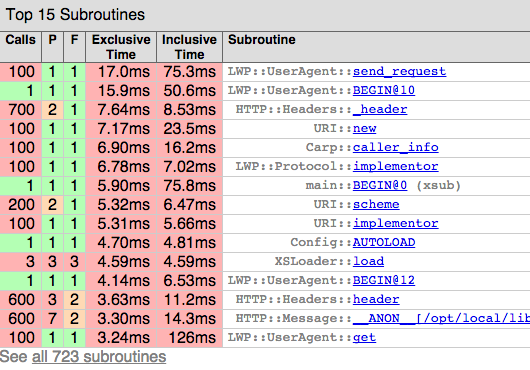
\includegraphics[width=10cm]{lectures/L12/nyt1.png}
\end{figure}


Профайлер замерил время выполнения всех функций, сколько раз они запускались и так далее. Функции отсортированы по времени исполнения и по умолчанию показаны только 15 из них.

\subsection{Inclusive и exclusive время исполнения}
Разница между inclusive и exclusive временем следующая. Пусть выполняется некоторая функция \verb|foo()|, которая вызывает дважды функцию \verb|bar()|.
\begin{figure}[H] % Картинка
	\centering
	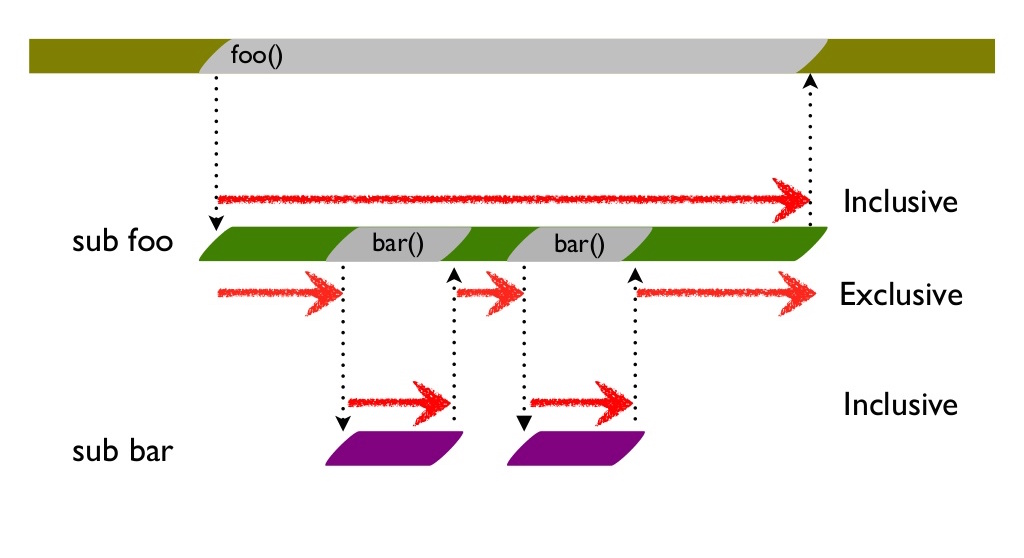
\includegraphics[width=10cm]{lectures/L12/inclusive-exclusive.jpg}
\end{figure}
Тогда inclusive time --- это время от входа в функцию до выхода из функции \verb|foo()|. Пока функция \verb|foo()| исполнялась, она исполняла другие функции. Соответственно время, которое было потрачено непосредственно на sub foo за вычетом вызовов других функций называется exclusive time. Практическим следствием отсюда является тот факт, что если у некоторой функции iclusive time большой, а exclusive time --- значительно меньше, то тормозит не она, а какая-то еще функция, которую она вызывает.

\subsection{Режим start=init}
От функций, которые исполняются один раз, в профиле можно избавиться, запустив профилировщик в режиме \verb|start=init|:
\begin{verbatim}
$ NYTPROF=start=init \
  perl -d:NYTProf -MLWP::UserAgent -E \
 'LWP::UserAgent->new->get("https://mail.ru/")
 for 1..100;'
$ nytprofhtml
\end{verbatim}
Здесь флаг \verb|start| задает момент, когда нужно запустить профилировщик. В данном случае он запускается после того, как выполнены все \verb|use|'ы, \verb|BEGIN|'ы и так далее. В результате получаются следующие результаты измерений:
\begin{figure}[H] % Картинка
	\centering
	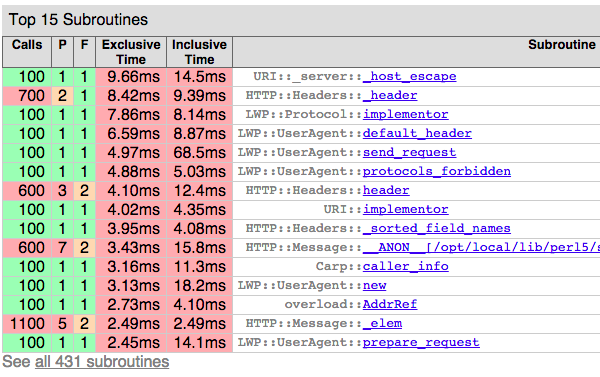
\includegraphics[width=10cm]{lectures/L12/nyt2.png}
\end{figure}

\subsection{Режим start=no}
В режиме \verb|start=no| профилировщик не запускается сам. После того, как все будет подготовлено, он будет запущен с помощью модуля \verb|DB|. Модуль \verb|DB| позволяет управлять дебаггером, в частности включать и выключать профилирование.

В данном конкретном случае не важно, сколько времени занимает загрузка модулей и создание объекта, а важно, чтобы определенный участок работал быстро:
\begin{verbatim}
$ NYTPROF=start=no \
  perl -d:NYTProf -MLWP::UserAgent -E \
 'my $ua = LWP::UserAgent->new;
  DB::enable_profile();
  $ua->get("https://mail.ru/") for 1..100;
  DB::disable_profile();'
$ nytprofhtml
\end{verbatim}
\begin{figure}[H] % Картинка
	\centering
	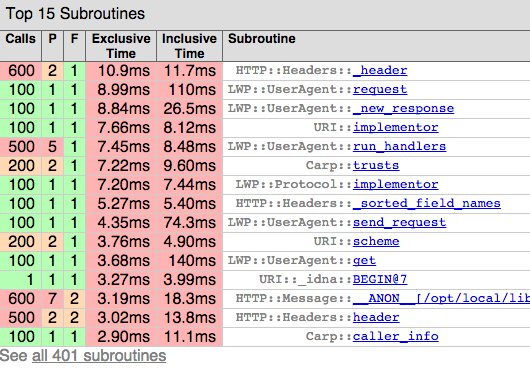
\includegraphics[width=10cm]{lectures/L12/nyt3.png}
\end{figure}
Теперь в профиле не содержится создание объекта и <<в топ вылезли>> функции \verb|_header| и \verb|request|. 
\begin{figure}[H] % Картинка
	\centering
	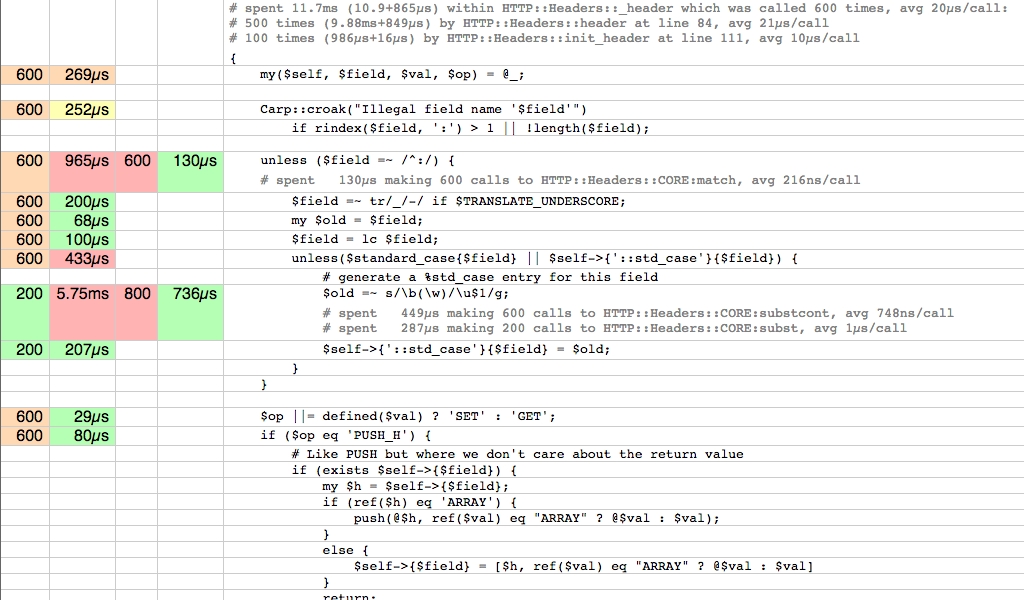
\includegraphics[width=13cm]{lectures/L12/nyt4.png}
\end{figure}
Причем inclusive time у функции \verb|request| значительно больше exclusive time. Эта разница обусловлено временем ожидания ввода-вывода в функции request.

\subsection{Flame Graph}
Flame Graph позволяет визуально увидеть, на что идет потраченное время.
\begin{figure}[H] % Flame Graph
	\centering
	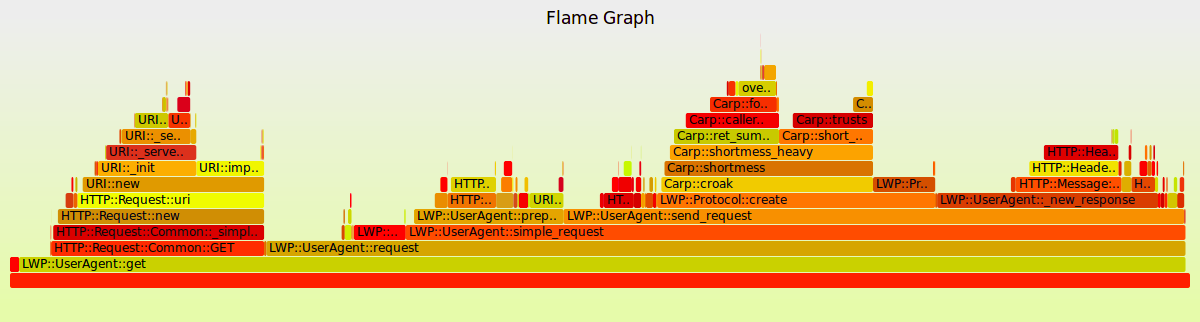
\includegraphics[width=15cm]{lectures/L12/flame.png}
\end{figure}
На этой картинке изображено суммарное время исполнения программы и по частям на что оно ушло. Причем на каждую вещь можно кликать и смотреть, из чего она состояла. Можно посмотреть, сколько раз вызывалась конкретная функция и сколько времени занимало исполнение конкретных строк.
\begin{figure}[H]
\end{figure}
\verb|NYTProf| пишет, сколько времени он провел внутри этой функции, сколько раз она вызывалась, какое среднее время исполнения функции, а также кто ее вызывал:
\begin{verbatim}
spent 11.7ms (10.9+865µs) within
    HTTP::Headers::_header which was called
    600 times, avg 20µs/call:
    500 times (9.88ms+849µs)
        by HTTP::Headers::header at line 84,
        avg 21µs/call
    100 times (986µs+16µs)
        by HTTP::Headers::init_header at line 111,
        avg 10µs/call
\end{verbatim}
Также под каждую строчку он пишет, сколько времени он проводил в конкретных вызовах. Вызов regexp'ов присутствует в виде функций \verb|CORE:match|, \verb|CORE:substcont| и \verb|CORE:subst|.
\begin{minted}{perl}
unless ($field =~ /^:/)
    # spent   130µs making 600 calls to
    HTTP::Headers::CORE:match, avg 216ns/call

$old =~ s/\b(\w)/\u$1/g;
    # spent   449µs making 600 calls to
        HTTP::Headers::CORE:substcont,
        avg 748ns/call
    # spent   287µs making 200 calls to
        HTTP::Headers::CORE:subst,
        avg 1µs/call
\end{minted}


\section{Оптимизация}
\subsection{Правила оптимизации}
Первое правило оптимизации --- не оптимизируйте программы. Второе правило оптимизации программ --- не оптимизируйте программы, пока это не понадобится. Большая часть проблем в софте возникает из-за того, что кто-то начинает оптимизировать программы раньше, чем это реально понадобилось. К этим проблемам относятся:
\begin{itemize}
  \item Превращение программы в нечитаемый код
  \item Программа превращается в огромный код
  \item Программу становится сложно поддерживать
  \item Делается ошибочное допущение без проверки
\end{itemize}

\subsection{Порядок профилирования и оптимизации программы}
Tim Bunce описал правила, как правильно профилировать программу:
\begin{enumerate}
    \item Даём репрезентативную нагрузку
      Репрезентативной нагрузкой называется нагрузка, которая соответствует тому окружению, в котором будет работать ваше приложение.
    \item Смотрим общее время функций
      Нужно адекватно оценивать возможности железа и perl при оценке времени.
    \item Время выглядит адекватно?
      Должна ли программа должна работать во много раз быстрее?
    \item Исследуем самые медленные участки
      Для этого необходимо профилировать в разных режимах.
    \item Исправляем простые проблемы
      Сначала необходимо найти простые ошибки (по невнимательности или из-за простоты написания) и оптимизировать их.
    \item Профилируем заново
    \item Производительность хорошая? СТОП!
    \item Повторите 1-2 раза
    \item Переходите к другим улучшениям.
\end{enumerate}

\subsection{Пример оптимизации}
Пусть дана строка из 1024 символов и две функции, которые вырезают первые 10 символов строки разными способами:
\begin{minted}{perl}
    my $str = "x"x1024;

    sub func1 {
      my $s = $str;
      substr($s,0,10,"");
    }

    sub func2 {
      my $s = $str;
      $s = substr($s,10);
    }
\end{minted}


Какая из двух функций будет работать быстрее? Из-за того, что 10 --- величина очень маленькая, и в perl действует хитрая оптимизация, которая позволяет смещать начало строки без реаллокации, функция \verb|func1| скорее всего будет работать быстрее. Но чтобы убедиться в этом, это нужно проверить. Также всегда нужно проверять скорость работы именно для тех данных и для того окружения и железа, которые будут в реальной работе.

\subsection{Модуль Benchmark}
Один из способов проверить --- использовать модуль \verb|Benchmark|. Если в качестве первого параметра подается положительное число, функция исполняется именно такое число раз. Если подано отрицательное значение, функция будет исполняться до тех пор, пока затраченное процессорное время не будет равно модулю этого значения.
\begin{minted}{perl}
  use Benchmark qw(:all);
  timethis(1e6,\&func1);
  timethis(-1,\&func1);
\end{minted}
Результат выполнения следующий:
\begin{verbatim}
timethis 1000000:  0 wallclock secs
    ( 0.20 usr +  0.01 sys =  0.21 CPU)
        @ 4761904.76/s (n=1000000)
(warning: too few iterations for a reliable count)
timethis for 1:  1 wallclock secs
    ( 1.02 usr +  0.00 sys =  1.02 CPU)
        @ 4665608.82/s (n=4758921)
\end{verbatim}
Помимо простого измерения модуль \verb|Benchmark| позволяет сравнивать между собой различные функции:
\begin{minted}{perl}
use Benchmark qw(:all);
timethese -1, {
    inplace => \&func1,
    copy    => \&func2,
};
\end{minted}
Результат выполнения следующий:
\begin{verbatim}
Benchmark: running copy, inplace for
    at least 1 CPU seconds...
copy:  2 wallclock secs
    ( 1.00 usr +  0.02 sys =  1.02 CPU)
        @ 4151600.98/s (n=4234633)
inplace:  1 wallclock secs
    ( 1.09 usr +  0.01 sys =  1.10 CPU)
        @ 4549606.36/s (n=5004567)
\end{verbatim}

\subsection{Модуль Dumbbench}
Модуль \verb|Dumbbench| позволяет выполнить серию начальных запусков.
\begin{minted}{perl}
use Dumbbench;
my $bench = Dumbbench->new(
    target_rel_precision => 0.005,
    initial_runs         => 50,
);
$bench->add_instances(
    Dumbbench::Instance::PerlSub
      ->new(name => 'inplace', code => \&func1),
    Dumbbench::Instance::PerlSub
      ->new(name => 'copy', code => \&func2),
);
$bench->run();
$bench->report();
\end{minted}
Результат выполнения следующий:
\begin{verbatim}
inplace: Ran 93 iterations (26 outliers).
inplace: Rounded run time per iteration:
    1.5462e-07 +/- 3.4e-10 (0.2%)
copy: Ran 56 iterations (6 outliers).
copy: Rounded run time per iteration:
    4.0881e-07 +/- 6.0e-10 (0.1%)
\end{verbatim}

\subsection{/dev/hands}
Помимо использования готовых модулей и утилит, можно реализовать процесс профилирования вручную. В perl есть функция \verb|times|, которая возвращает текущее потребление user time и system time. Тогда код будет иметь вид:
\begin{minted}{perl}
use List::Util qw(sum); my $N = 4e6;
my $cpu = sum((times)[0,1]);
func1() for 1..$N;
my $cpu1 = sum((times)[0,1]);
printf "%0.3fs CPU, %0.1fns/call\n",
$cpu1-$cpu, (1e9/$N)*($cpu1-$cpu);
func2() for 1..$N;
my $cpu2 = sum((times)[0,1]);
printf "%0.3fs CPU, %0.1fns/call\n",
$cpu2-$cpu1, (1e9/$N)*($cpu2-$cpu1);
\end{minted}
Результат выполнения следующий:
\begin{verbatim}
1.320s CPU, 330.0ns/call
1.460s CPU, 365.0ns/call
\end{verbatim}

\section{Оптимизация: Простые локальные изменения}

\begin{itemize}
\item Вынести постоянные выражения за пределы цикла
\begin{minted}{perl}
for (...) {
	my $a = 123;
	call_sub($a);
}

my $a = 123;
for (...) {
	call_sub($a);
}
\end{minted}
	\item Избегать повторения цепочек аксессоров
Следующий код:
\begin{minted}{perl}
Avoid->repeated()->chains()->of->accessors();
Avoid->repeated()->chains()->of->accessors();
Avoid->repeated()->chains()->of->accessors();
\end{minted}
можно оптимизировать введя новую переменную:
\begin{minted}{perl}
my $one = Avoid->repeated()->chains()->of;
$one->accessors();
$one->accessors();
$one->accessors();
\end{minted}
\item Не вызывайте те функции, которые можно не вызывать:
\begin{minted}{perl}
use constant DEBUG => 0;
my $unused = $self->get_something;
my $do_log = $logger->logging;
for (...) {
	$logger->log(...) if $do_log;
	do_debug(...) if DEBUG;
	...
}
\end{minted}

\item Выходите раньше, инициализируйте позже
\begin{minted}{perl}
sub {
    return unless @_;
    return 1 if @_ == 1;
    for (@_) { ... }
    ...
}
sub {
    if () { ... }
    elsif () { ... }
    else {
        return;
    }
}
\end{minted}

\item Избегайте ненужных проверок
\begin{minted}{perl}
- return exists $hash{$something}{$key}
-             ? $hash{$something}{$key}
-             : undef

+ return $hash{$something}{$key}
\end{minted}
\item Используйте аргументы без распаковки в наиболее часто вызываемых функциях
\begin{minted}{perl}
sub add ($$) {
    return $_[0] + $_[1]
}
\end{minted}

\item Внести цикл под вызов
\begin{minted}{perl}
$object->walk($_) for @dogs;
$object->walk_that(\@dogs);
\end{minted}
\end{itemize}


\section{Оптимизация: значительные изменения}
Попытайтесь найти быстрый модуль, чем тот, что используется сейчас. На сайте \url{http://neilb.org/reviews/} регулярно проводятся обзоры модулей и сравнивает их по потреблению ресурсов и по функционалу.

Еще один неочевидный способ повысить производительность --- обновить и/или пересобрать perl:
\begin{itemize}[nosep]
	\item Сборка без тредов дает до +30\%
	\item Сборка без отладки дает до +5\%
	\item 5.10 -> 5.16 может дать до +15\%
	\item 5.16 -> 5.20 может дать до +20\%
\end{itemize}


Оптимизация алгоритмов
\[    O(n^2) \to O(n \log n) \to O(n) \to O(\log n) \to O(1) \]

Переписывание <<горячих>> участков на XS

% TODO 1:37:32
\section{Память}
Второй ресурс, который становится критичен, это память. При создании небольших приложений потреблению памяти обычно не уделяется внимание. Если процесс должен обрабатывать большие объемы данных, вопрос потребления памяти становится особенно актуален.

Классический пример утечки памяти --- циклическая ссылка.
\begin{minted}{perl}
my $x;$x = \$x; # << selfref

my $h = {};
$h->{key} = $h; # << cyclic ref

my $s;$s = sub {
    $s->(); # << ref by closure
};
\end{minted}
При создании циклической ссылки сборщик мусора в perl уже не может уничтожить данную переменную автоматически. Это связано с тем, что переменная ссылается сама на себя и счетчик ссылок никогда не достигнет нуля.

Для обнаружения утечек используется модуль \verb|Devel::Leak|.
\begin{minted}{perl}
use Devel::Leak;
Devel::Leak::NoteSV($handle);

my $x;$x = \$x;
my $h = {};$h->{key} = $h;
my $s;$s = sub {$s->();};

Devel::Leak::CheckSV($handle);
\end{minted}
Сначала создается заметка, затем исполняется требуемый код и вызываеся проверка на этой заметке:
\begin{minted}{perl}
new 0x7fc84b021b28 :
new 0x7fc84b021b40 :
new 0x7fc84b021b58 :
new 0x7fc84b021b70 :
new 0x7fc84b021c00 :
new 0x7fc84b021c18 :
new 0x7fc84b004ce8 :
new 0x7fc84b004ec8 :
\end{minted}
Если perl собран с флагом -DDEBUGGING (то есть с отладкой), вывод будет более подробный:
\begin{minted}{bash}
new 0x2410de8 : SV = PVHV(0x2416e40) at 0x2410de8
  REFCNT = 2
  FLAGS = (SHAREKEYS)
  ARRAY = 0x24aa640  (0:7, 1:1)
  hash quality = 100.0%
  KEYS = 1
  FILL = 1
  MAX = 7
  RITER = -1
  EITER = 0x0
new 0x2410f68 : SV = IV(0x2410f58) at 0x2410f68
  REFCNT = 1
  FLAGS = (ROK)
  RV = 0x2410de8
    SV = PVHV(0x2416e40) at 0x2410de8
      REFCNT = 2
      FLAGS = (SHAREKEYS)
      ARRAY = 0x24aa640  (0:7, 1:1)
\end{minted}
По этой информации уже можно понять, что именно утекло.

Другой способ найти утечку памяти --- использовать переменную, в которой хранится число используемых SV:
\begin{minted}{perl}
int checkpoint = PL_sv_count;

/* ...some leaky code... */

printf("leaked by %d SV's",
    PL_sv_count - checkpoint);
\end{minted}
Если код при своем повторении не создает лишние SV, то есть все что он создал, он потом уничтожил, то будет выведен ноль.

При использовании Linux, утечку памяти можно обнаружить вручную:
\begin{minted}{bash}
/proc/[pid]/statm
  Provides information about memory usage.

  size   total program size
         (same as VmSize in /proc/[pid]/status)
  resident   resident set size
         (same as VmRSS in /proc/[pid]/status)
  share  shared pages (from shared mappings)
  text   text (code)
  lib    library (unused in Linux 2.6)
  data   data + stack
  dt     dirty pages (unused in Linux 2.6)
\end{minted}
Для этого удобно создать функцию mem:
\begin{minted}{perl}
use POSIX qw( _SC_PAGESIZE sysconf );
my $PG = sysconf(_SC_PAGESIZE);
sub mem () {
    open my $f,'<:raw','/proc/self/statm';
    my ($all,$rss,$shr,$txt,$lib,$data) =
    map $_*$PG, split /\s+/, scalar <$f>;
    return $data;
}

my $before = mem();
for (1..1e5) {
    my %h;$h{key} = \%h;
}
my $after = mem();
printf "Lost %0.1fM\n",
    ($after-$before)/1024/1024;
\end{minted}
В результате исполнения кода будет выведено количество потерянной памяти после прогона:
\begin{minted}{bash}
Lost 17.7M
\end{minted}
В связи с особенность выделения памяти в perl, не всегда увеличение используемой памяти значит утечку. В этом случае следует увеличить число итерации --- в случае утечки память будет расти линейно в зависимости от номера итерации.

Если используется не Linux, можно воспользоваться модулем Proc::ProcessTable:
\begin{minted}{perl}
use Proc::ProcessTable;
my $t = Proc::ProcessTable->new();

for my $p ( @{ $t->table } ) {
  next unless $$ == $p->pid;
  say $p->pid," ", $p->size;
}
\end{minted}
Если утечка памяти происходит в модуле XS:
\begin{minted}{c++}
void test(SV *var)
PPCODE:
    SV *leaky = newSVpvs("dummy");
    XSRETURN_UNDEF;
\end{minted}
После использования Devel::Leak:
\begin{minted}{perl}
use Devel::Leak;
Devel::Leak::NoteSV(my $chk);
LeakTest::test($smth);
Devel::Leak::CheckSV($chk);
\end{minted}
оказалось, что есть утечка:
\begin{minted}{bash}
new 0x1496a68 :
\end{minted}
В этом случае есть способ определять место утечки с помощью опорной переменной:
\begin{minted}{c++}
void test(SV *var)
PPCODE:
    SV *leaky = newSVpvs("dummy");
    printf("var = %p\n",var);
    SV * ghost = (SV *) ( (char *)var + 0 );
    sv_dump( ghost );
    XSRETURN_UNDEF;
\end{minted}
Таким образом, известен адрес опорной переменной и утекающей переменной.
\begin{minted}{bash}
var = `0x2075c38`
SV = NULL(0x0) at `0x2075c38`
  REFCNT = 1
  FLAGS = (PADMY)
new `0x2058a68` :
\end{minted}
Можно подсчитать разницу:
\begin{minted}{bash}
0x2058a68 - 0x2075c38 = -119248
\end{minted}
и подставить эту разницу обратно в код:
\begin{minted}{c++}
void test(SV *var)
PPCODE:
    SV *leaky = newSVpvs("dummy");
    printf("var = %p\n",var);
    SV * ghost = (SV *) ( (char *)var - `119248` );
    sv_dump( ghost );
    XSRETURN_UNDEF;
\end{minted}
Поскольку код не изменился (только изменилось число), адреса не сдвинутся. После запуска опорная переменная останется на том же месте, а также становится известна информация об утекшей переменной:
\begin{minted}{bash}
var = 0x20f2c38
SV = PV(0x20d3cf0) at `0x20d5a68`
  REFCNT = 1
  FLAGS = (POK,pPOK)
  PV = 0x21ab7a0 "dummy"\0
  CUR = 5
  LEN = 16
new `0x20d5a68` :
\end{minted}
Чтобы исправить утечку, необходимо добавить \verb|sv_2mortal|:
\begin{minted}{c}
void test(SV *var)
PPCODE:
    SV *leaky = sv_2mortal(newSVpvs("dummy"));
    printf("var = %p\n",var);
    SV * ghost = (SV *) ( (char *)var - `119248` );
    sv_dump( ghost );
    XSRETURN_UNDEF;
\end{minted}
\begin{minted}{bash}
var = 0x20f2c38
SV = PV(0x20d3cf0) at `0x20d5a68`
  REFCNT = 1
  FLAGS = (POK,pPOK)
  PV = 0x21ab7a0 "dummy"\0
  CUR = 5
  LEN = 16
\end{minted}


Self-referenced closure:
\begin{minted}{perl}
my $cb; $cb = sub {
    something_async sub {
        $cb->();
    };
};
$cb->();
\end{minted}
В perl есть возможность создавать слабые ссылки. То есть есть ссылка на какой-то блок, которая не удерживает +1 на счетчике ссылок. Not very self-referenced closure:
\begin{minted}{perl}
use Scalar::Util qw(weaken);
my $cb; $cb = sub {
    my $cb = $cb or return;
    something_async sub {
        $cb->();
    };
};
$cb->(); # initial call
# or $cb->() for 1..$N
weaken($cb);
\end{minted}

Destruction tracking:
\begin{minted}{perl}
use Guard;
{
    my %struct;
    # ...
    $struct{__tmp} = guard {
        warn "Object destroyed";
    }
}
\end{minted}
\begin{minted}{bash}
Object destroyed at - line 6.
\end{minted}

\begin{minted}{perl}
use Guard;
{
    my %struct;
    # ...
    $struct{__} = \%struct;
    $struct{__tmp} = guard {
        warn "Object destroyed";
    }
}
\end{minted}
\begin{minted}{bash}
Object destroyed at - line 7 `during global destruction`.
\end{minted}


\section{Файловые дескрипторы}
Последний ресурс --- файловые дескрипторы: файл может быть открыт, но после использования не закрыт. Чтобы обнаружить эту проблему, существует простой ручной способ.

При открытии нового файла дается максимальное значение дескриптора из тех, которые сейчас есть. Следовательно, если какой-то код открывает и закрывает все дескрипторы, то если повторно открыть какой-то файл и закрыть его, будет получен один и тот же номер дескриптора.

\begin{minted}{perl}
open my $f,'<:raw', '/dev/null';
my $before = fileno($f);
close ($f);

# ...leaky code ...

open my $f,'<:raw', '/dev/null';
my $after = fileno($f);
close ($f);

printf "Leaked by %d descriptors\n",
    $after - $before;
\end{minted}
В результате этого кода будет получено количество потеряных дескрипторов. Вместо открытия файла можно воспользоваться встроенной переменной \verb|$SYSTEM_FD_MAX|:
\begin{minted}{perl}
# perlvar: $SYSTEM_FD_MAX
my $before = $^F;
# ...leaky code ...
my $after = $^F;
\end{minted}
Эти два подхода эквивалентны.

\end{document}
